
\section*{부록 개요}

이 부록은 본 논문을 뒷받침하는 보충 자료를 제공한다. 데이터 전처리 파이프라인, 모델 및 학습 설정, 모든 과제의 실험 설정을 자세히 설명하고, 하이퍼파라미터 민감도 분석, 전체 결과 표, 예측 사례를 포함한 추가 결과를 제시한다.

\section{관련 연구}

\subsection{시계열 토큰화}

The recent success of large, token-based models has spurred a growing interest in discretizing continuous time series. This tokenization process is pivotal for adapting such architectures for time series analysis, yet dedicated research in this area remains sparse. Early efforts like Chronos~\cite{ansari2024chronos} employ scaling and uniform quantization, while TOTEM~\cite{talukder2024totem} utilizes a Vector Quantized Variational Autoencoder (VQ-VAE)~\cite{van2017neural}—a seminal approach that maps encoder outputs to learned discrete latent codes—for codebook-based tokenization. Given this nascent landscape, we draw inspiration from the more mature field of visual tokenization. Beyond the foundational VQ-VAE, innovations include Lookup-Free Quantization (LFQ)~\cite{yu2023language}, achieving high-fidelity reconstruction via an implicit codebook without explicit lookups. Binary Spherical Quantization (BSQ)~\cite{zhao2024image} advances implicit codebooks using spherical projection for an exponentially growing vocabulary, offering bounded quantization error and improved trainability over LFQ. Further, Index Backpropagation Quantization (IBQ)~\cite{shi2025scalableimagetokenizationindex} tackles codebook collapse by making all code entries differentiable, enabling stable joint optimization of large-scale codebooks and the visual encoder. While primarily designed for visual data, these methods can also be applied to discretize general multivariate time series.

\subsection{범용 시계열 파운데이션 모델}

The paradigm of time series analysis has recently been reshaped by Time Series Foundation Models (TSFMs), drawing inspiration from the success of Large Language Models in leveraging massive pre-trained Transformers. These models are trained on vast, multi-domain corpora—some with over a hundred billion data points—to achieve remarkable zero-shot or few-shot performance on general forecasting benchmarks. This versatility is enabled by diverse architectures, including decoder-only models like Lag-Llama~\cite{rasul2023lag}, TimesFM~\cite{das2024decoder}, Timer~\cite{liu2024timer}, Time-MoE~\cite{xiaoming2025time}, and Sumdial~\cite{liu2025sundial}; encoder-only frameworks like MOMENT~\cite{goswami2024moment} and Moirai~\cite{woo2024unified}; encoder-decoder structures such as TimeGPT~\cite{garza2023timegpt}; and models with modified Transformer blocks for multi-task learning like UniTS~\cite{gao2024units}. At the input level, they employ generic representations such as direct value patching (e.g., TimesFM~\cite{das2024decoder}, MOMENT~\cite{goswami2024moment}), value quantization into a fixed vocabulary (e.g., Chronos~\cite{ansari2024chronos}), or treating consecutive time points as tokens (e.g., Timer~\cite{liu2024timer}). Several of these models also extend to probabilistic forecasting (e.g., Lag-Llama~\cite{rasul2023lag}, Moirai~\cite{woo2024unified}, Chronos~\cite{ansari2024chronos} and Sumdial~\cite{liu2025sundial}).

However, the very generality that drives their success on broad benchmarks becomes a limitation in specialized domains. To provide a concrete comparison, we summarize key attributes of prominent TSFMs in Table~\ref{tab:tsfm_comparison}. A important observation from the table is the minuscule proportion of financial data within the pre-training corpora of these general-purpose models, with most dedicating less than 1\% of their data to this domain. This data imbalance means that the unique structural properties, non-stationarity, and complex dynamics of financial K-line sequences are largely overlooked or averaged out during pre-training, often resulting in suboptimal performance for financial tasks. To address this fundamental gap in pre-training, we introduce Kronos, a foundation model built from the ground up on a massive corpus composed exclusively of financial K-line data.

\subsection{금융 시계열 파운데이션 모델}

The development of foundation models specifically for finance time series is a nascent but rapidly growing field. These efforts can be divided into two main streams. The first focuses on general financial time series, including K-line data. For instance, PLUTUS~\cite{xu2024plutus} introduces an invertible embedding and multi-scale temporal attention, pre-trained on massive datasets to uncover market regularities. DELPHYNE~\cite{ding2025delphyne} is designed explicitly to counteract the negative transfer from non-financial data. While promising, neither of these works has released their code or models, precluding direct empirical comparison. The second stream targets order flow data, where models like MarketGPT~\cite{wheeler2024marketgpt} and MarS~\cite{li2024mars} act as generative engines for realistic market simulation. These pioneering efforts validate the value of domain-specific pre-training. However, K-line data possesses broader applicability than order flow, as it is readily available across all markets and suitable for diverse time horizons where order flow data is often inaccessible. Despite its central importance, a versatile and open-source foundation model for K-line analysis remains a notable gap. We introduce Kronos to fill this void, offering a unified, scalable framework designed specifically for financial K-line data.

\begin{table*}[t]
\centering

\resizebox{\textwidth}{!}{%
\begin{tabular}{@{}lllccl@{}}
\toprule
\textbf{Model} & \textbf{아키텍처} & \textbf{토큰화} & \textbf{확률적} & \textbf{금융 데이터 비율(추정)} & \textbf{주요 도메인} \\ \midrule
\textbf{Kronos (Ours)} & \textbf{Decoder-only} & \textbf{Discrete (BSQ)} & \textbf{Yes} & \textbf{100\%} & \textbf{Financial K-lines} \\
\midrule
Sundial~\cite{liu2025sundial} & Decoder-only & Continuous & Yes & 1.02\% & General \\
Time-MoE~\cite{xiaoming2025time} & Decoder-only & Continuous & No & $<$0.01\% & General \\
Moirai~\cite{woo2024unified} & Encoder-only & Continuous & Yes & 0.10\% & General \\
MOMENT~\cite{goswami2024moment} & Encoder-only & Continuous & No & 1.60\% & General \\
Chronos~\cite{ansari2024chronos} & Encoder-Decoder & Discrete (Quantization) & Yes & 0.45\% & General \\
Timer~\cite{liu2024timer} & Decoder-only & Continuous & No & 0.03\% & General \\
TimesFM~\cite{das2024decoder} & Decoder-only & Continuous & No & $<$0.01\% & General \\
UniTS~\cite{gao2024units} & Encoder-only & Continuous & No & Unknown & General \\
Lag-Llama~\cite{rasul2023lag} & Decoder-only & Continuous & Yes & 0.01\% & General \\
% TimeGPT~\cite{garza2023timegpt} & Encoder-Decoder & Continuous & No & Unknown & General \\
\bottomrule
\end{tabular}%
}
\caption{시계열 파운데이션 모델 비교. 이 표는 아키텍처 선택, 토큰화 방법, 확률적 예측 기능, 그리고 사전학습 말뭉치에서 금융 데이터가 차지하는 추정 비율을 강조한다.}
\label{tab:tsfm_comparison}
\end{table*}

\section{데이터셋 세부 사항}
\label{sec:dataset_details}

\begin{table}[t]
\centering
\small

\setlength{\tabcolsep}{4pt} % Reduce space between columns
\resizebox{\columnwidth}{!}{%
\begin{tabular}{l c c cc}
\toprule
& & & \multicolumn{2}{c}{\textbf{Max. Consecutive Bars}} \\
\cmidrule(lr){4-5}
\textbf{주기} & \textbf{\begin{tabular}[c]{@{}c@{}}Min. Length \\ (bars)\end{tabular}} & \textbf{\begin{tabular}[c]{@{}c@{}}Price Jump \\ Threshold\end{tabular}} & \textbf{비유동} & \textbf{정체} \\
\midrule
1min    & 2048 & 0.10 & 15 & 45 \\
5min    & 1024 & 0.15 & 3 & 10 \\
10min   & 512  & 0.15 & 3 & 6  \\
15min   & 512  & 0.15 & 2 & 5  \\
20min   & 512  & 0.15 & 2 & 5  \\
30min   & 512  & 0.20 & 2 & 3  \\
40min   & 256  & 0.20 & 1 & 3  \\
60min   & 256  & 0.20 & 1 & 3  \\
2H      & 128  & 0.25 & 1 & 3  \\
4H      & 128  & 0.25 & 1 & 3  \\
Daily   & 128  & 0.30 & 1 & 3  \\
Weekly  & 16   & 0.50 & 0 & 2  \\
\bottomrule
\end{tabular}}
\caption{저품질 데이터 필터링 파이프라인의 주기별 파라미터. 임계값은 서로 다른 시간 주기의 고유한 동학을 반영하도록 조정된다.}
\label{tab:cleaning_parameters}
\end{table}

\subsection{데이터 전처리와 정제}
\label{appendix:data_cleaning}

This section details the preprocessing and cleaning pipeline applied to the large-scale K-line dataset used for pre-training. The dataset is aggregated from over 40 exchanges across more than 30 countries, comprising a diverse range of asset classes at multiple temporal frequencies (1-minute to weekly). A statistical overview is provided in Table~\ref{tab:dataset_overview}. The integrity of large-scale pre-training is contingent upon high-quality input data. Raw K-line series, however, are frequently contaminated by artifacts stemming from low liquidity, price limits, or data feed errors. To mitigate the impact of such issues, we implement a rigorous, two-stage pipeline designed to process missing values and filter out low-quality data segments.

\begin{algorithm}[t]
\caption{저품질 구간 필터링 파이프라인}
\label{alg:segment_filtering}
\begin{algorithmic}[1]
\Statex \textbf{입력:} Raw K-line series $S_{raw}$, Parameter set $\Theta$ for a given frequency (from Table~\ref{tab:cleaning_parameters})
\Statex \textbf{출력:} A set of clean K-line segments $\mathcal{C}$

\Function{FilterLowQualitySegments}{$S_{raw}, \Theta$}
    \State $\mathcal{C} \leftarrow \emptyset$ \Comment{Initialize the set of final clean segments}
    \State $\mathcal{S}_{initial} \leftarrow \text{PartitionByPriceJumps}(S_{raw}, \Theta_{\text{jump}})$ \Comment{Split by structural breaks}

    \ForAll{segment $S$ in $\mathcal{S}_{initial}$}
        \State $M_{illiquid} \leftarrow \text{FlagConsecutiveIlliquid}(S, \Theta_{\text{illiquid}})$ \Comment{Identify illiquid periods}
        \State $M_{stagnant} \leftarrow \text{FlagConsecutiveStagnant}(S, \Theta_{\text{stagnant}})$ \Comment{Identify stagnant periods}
        \State $M_{invalid} \leftarrow M_{illiquid} \lor M_{stagnant}$ \Comment{Combine masks for all invalid points}

        \State $\mathcal{S}_{clean} \leftarrow \text{ExtractValidSubsequences}(S, M_{invalid})$ \Comment{Split segment on invalid boundaries}

        \ForAll{subsequence $S_{sub}$ in $\mathcal{S}_{clean}$}
            \If{$\text{Length}(S_{sub}) \ge \Theta_{\text{min\_len}}$}
                \State $\mathcal{C} \leftarrow \mathcal{C} \cup \{S_{sub}\}$ \Comment{Add valid, sufficiently long segment}
            \EndIf
        \EndFor
    \EndFor

    \State \textbf{return} $\mathcal{C}$
\EndFunction
\end{algorithmic}
\end{algorithm}

\subsubsection{결측값 처리}
We employ a field-specific strategy to handle missing values, which are typically represented as `NaN' (Not a Number) or `Inf' (Infinity).

\begin{itemize}
    \item \textbf{Price Fields (Open, High, Low, Close):} For price-related fields, we treat missing values as hard boundaries. Inspired by TimeMOE~\cite{xiaoming2025time}, we partition the time series into contiguous, valid sub-sequences at each occurrence of a missing price value. This approach ensures that each resulting segment maintains its internal temporal integrity without unwarranted imputation.
    \item \textbf{Volume and Amount Fields:} In contrast, for volume and amount fields, which primarily serve as auxiliary covariates, we impute missing values with zero. To enhance model robustness to sparse or unavailable volumetric data, we introduce a regularization technique: during training, both volume and amount are randomly set to zero for 5\% of the input samples. This encourages the model to learn to make effective predictions from price information alone.
\end{itemize}

\subsubsection{저품질 구간 필터링}
Beyond addressing discrete missing values, our pipeline systematically identifies and removes entire segments of low-quality data. This is achieved through a multi-stage filtering process where tolerance thresholds are dynamically adjusted according to the data's temporal frequency, as detailed in Table~\ref{tab:cleaning_parameters}. The procedure, formalized in Algorithm~\ref{alg:segment_filtering}, consists of the following steps:

\begin{itemize}
    \item \textbf{Structural Break Segmentation.} The initial filtering stage partitions the series based on significant price discontinuities. We identify these breaks by calculating the relative price jump between the previous bar's close and the current bar's open ($| \text{open}_t / \text{close}_{t-1} - 1 |$). If this jump exceeds a frequency-specific threshold, the sequence is split. This step effectively isolates artifacts arising from events such as contract rollovers, stock splits, or dividend distributions.
    \item \textbf{Filtering of Illiquid Periods.} Within each segment from the previous step, we screen for periods of sustained illiquidity. A bar is deemed illiquid if its trading volume is zero or near-zero. If the number of consecutive illiquid bars exceeds a frequency-dependent threshold, the corresponding period is flagged as invalid.
    \item \textbf{Filtering of Price Stagnation.} We apply a similar method to filter periods of price stagnation, where the closing price remains constant over an extended duration. This often indicates potential data feed issues or market inactivity. If the length of a stagnant streak surpasses its frequency-specific tolerance, it is also flagged as an invalid period.
    \item \textbf{Final Segment Validation.} After flagging all illiquid and stagnant periods, the initial segments are further split at the boundaries of these flagged regions. Finally, only the resulting sub-segments that meet the frequency-specific minimum length requirement ($\Theta_{\text{min\_len}}$ in Table~\ref{tab:cleaning_parameters}) are retained for the final pre-training dataset. This ensures each sample is sufficiently long to support meaningful model learning.
\end{itemize}

\section{구현 세부 사항}
\label{sec:implementation_details}

In this section, we provide further details on the implementation of Kronos, covering data preprocessing, model architecture, and configurations for training and inference.

\subsection{입력 전처리}
\label{sec:input_processing}
Each input K-line sequence $\mathbf{x} = (\mathbf{x}_1, \mathbf{x}_2, \dots, \mathbf{x}_T)$, where $\mathbf{x}_t \in \mathbb{R}^D$, is normalized in a two-step procedure before being passed to the tokenizer. First, we apply z-score normalization independently to each of the $D$ feature dimensions (e.g., Open, High, Low, Close, Volume and Amount). Second, to mitigate the potential impact of extreme outliers on training stability, the normalized values are clipped to the range $[-5, 5]$. This process ensures that all input features have a consistent scale while preserving the model's robustness against anomalous data points.

\begin{table*}[t!]
  \centering

  \resizebox{0.9\textwidth}{!}{%
  \begin{tabular}{@{}lcccccc@{}}
    \toprule
    \textbf{Model} & \textbf{FFN Dropout} & \textbf{Residual Dropout} & \textbf{Attention Dropout} & \textbf{Token Dropout} & \textbf{Learning Rate} & \textbf{Weight Decay} \\
    \midrule
    $\text{Kronos}_{small}$ & 0.25 & 0.25 & 0.1 & 0.1 & \num{1e-3} & 0.01 \\
    $\text{Kronos}_{base}$  & 0.20 & 0.20 & 0.0 & 0.0 & \num{5e-4} & 0.05 \\
    $\text{Kronos}_{large}$ & 0.00 & 0.00 & 0.0 & 0.0 & \num{2e-4} & 0.10 \\
    \bottomrule
  \end{tabular}%
  }
  \caption{Kronos 모델 계열의 하이퍼파라미터 설정. 모든 모델은 AdamW 옵티마이저로 학습된다.}
  \label{tab:training_params}
\end{table*}

\subsection{모델 아키텍처}

\paragraph{시간 임베딩.} To capture cyclical patterns inherent in financial markets, such as intraday, weekly, and monthly seasonality~\cite{ozenbas2008intra,kohli1992week}, we incorporate learnable temporal embeddings. We extract five time-related features for each K-line entry: minute-of-day, hour-of-day, day-of-week, day-of-month, and month-of-year. Each feature is mapped to a dense vector via a dedicated embedding layer. These temporal embeddings are summed and then added to the input representation of each corresponding token, providing the model with explicit temporal context.

\paragraph{K-line 토큰화.} The tokenizer's autoencoder is designed to be lightweight. The encoder and decoder each consist of 3 Transformer layers, with a model dimension of 256, a feed-forward network dimension of 512, and 4 attention heads. Following the official open-source implementation of BSQ\footnote{\url{https://github.com/zhaoyue-zephyrus/bsq-vit}}, we configure the key quantization hyperparameters as follows: a commitment weight $\beta=0.05$, entropy penalty weights $\gamma_0=1.0$ and $\gamma=1.1$, and an overall entropy scale $\zeta=0.05$. The balancing hyperparameter $\lambda$ for the quantization loss in our objective is set to 1. The quantization group size is set to 5 for tractable entropy computation.

\paragraph{Transformer 블록 아키텍처.} To encode the sequential nature of the data, we employ causal self-attention with Rotary Position Embeddings (RoPE)~\cite{su2024roformer}, which injects relative positional information. The attention operation is formulated as follows:
\begin{equation}
    \text{Attention}(Q, K, V) = \text{CausalMask}\left(\frac{Q' (K')^T}{\sqrt{d_k}}\right)V
\end{equation}
where $d_k$ is the dimension of the key vectors, and $\text{CausalMask}$ prevents attending to future positions. The matrices $Q'$ and $K'$ represent the original query and key matrices with RoPE transformations applied. Furthermore, we adopt the Pre-Layer Normalization (Pre-LN)~\cite{xiong2020layer} to improve training stability, specifically utilizing Root Mean Square Layer Normalization (RMSNorm)~\cite{zhang2019root} for its computational efficiency and performance.

\subsection{학습 설정}
The training hyperparameters are carefully selected for each model size to ensure a stable pre-training process. As model scale increases, we decrease the peak learning rate and dropout probability while increasing the weight decay. We employ the AdamW optimizer~\cite{loshchilov2017decoupled} and a cosine learning rate schedule with a linear warm-up phase. The learning rate warms up from 10\% of its peak value over the first 15,000 training steps. Table~\ref{tab:training_params} details the specific hyperparameter settings for each model variant.

\begin{table*}[t!]
\centering
\setlength{\tabcolsep}{4pt}

\begin{tabular}{lccc}
\toprule
\textbf{과제} & \textbf{온도 (T)} & \textbf{Top-p} & \textbf{추론 샘플 수 (N)} \\
\midrule
Price Series Forecasting      & 0.6 & 0.90 & 10 \\
Return Forecasting            & 0.6 & 0.90 & 10 \\
Realized Volatility Forecasting & 0.9 & 0.90 & 1 \\
Synthetic K-line Generation      & 1.0 & 0.95 & 1 \\
Investment  Simulation        & 0.6 & 0.90 & 10 \\
\bottomrule
\end{tabular}
\caption{다운스트림 과제의 추론 하이퍼파라미터. T는 샘플링 온도를, Top-p는 nucleus sampling을, N은 각 테스트 인스턴스마다 생성되는 추론 샘플 수를 나타낸다.}
\label{tab:inference_hyperparams}
\end{table*}

\subsection{추론 하이퍼파라미터}
The generation process at inference time is controlled by temperature scaling ($T$) and nucleus (top-$p$) sampling. The optimal choice of these hyperparameters is task-dependent. For example, forecasting tasks generally benefit from lower temperatures to reduce randomness, whereas generative tasks may require higher temperatures to increase diversity. A detailed analysis of hyperparameter sensitivity is available in Appendix~\ref{sec:sampling_hyperparams}. The inference hyperparameters used for each task are detailed in Table~\ref{tab:inference_hyperparams}.

\subsection{사전학습 데이터 재균형화}
The raw pre-training corpus exhibits a natural imbalance across asset classes, with equities being more prevalent than cryptocurrencies, futures, and foreign exchange (forex) assets. To prevent potential underfitting on these less-represented classes, we apply strategic resampling to the training data. Specifically, we increase the sampling weights for data from crypto, futures, and forex markets. This rebalancing ensures the model gains more balanced exposure to the diverse dynamics across different financial instruments.

\section{실험 설계와 구현}
\label{sec:exp_setup_details}

In this section, we present the comprehensive experimental design and implementation for the evaluation of Kronos. We begin by outlining the core evaluation tasks and their corresponding metrics. Next, we introduce the suite of baseline models used for comparison and detail their specific configurations. Finally, we provide a detailed account of the implementation for each experimental task, covering the datasets, parameters, and specific protocols used in our evaluation.

\subsection{과제와 평가 지표}
We evaluate Kronos on a diverse set of tasks that are central to quantitative finance. The tasks and their respective evaluation metrics are as follows:
\begin{itemize}
    \item \textbf{Price Series Forecasting:} We assess the model's ability to predict future price series. Performance is measured by the Information Coefficient (IC) and Rank Information Coefficient (RankIC) between the predicted and actual values.
    \item \textbf{Return Forecasting:} Similarly, we evaluate the model's proficiency in forecasting asset returns, also using IC and RankIC as the metrics to gauge predictive accuracy.
    \item \textbf{Realized Volatility Forecasting:} We use the model's high-frequency forecasts to estimate realized volatility. The accuracy of these estimations is evaluated using Mean Absolute Error (MAE) and the Coefficient of Determination ($R^2$).
    \item \textbf{Synthetic K-line Generation:} Following established practices in time series generation~\cite{yoon2019time}, we assess the quality of synthetic K-line sequences from three perspectives: \textit{diversity}, assessing how well the generated samples cover the distribution of the real data; \textit{fidelity}, assessing whether synthetic samples are indistinguishable from real data; and \textit{usefulness}, evaluating if synthetic data is as effective as real data for downstream predictive tasks (i.e., the Train-on-Synthetic, Test-on-Real paradigm).
    \item \textbf{Investment Simulation:} To measure the practical applicability of the model's forecasts, we perform backtesting simulations. The performance is reported using Annualized Excess Return (AER) and Information Ratio (IR).
\end{itemize}

\subsection{베이스라인과 설정}
For a rigorous evaluation, we benchmark Kronos against a comprehensive suite of 25 baseline models. These models are selected from prior works (e.g.,~\cite{xiaoming2025time,wang2024deep,yuan2024diffusion}) to represent a diverse range of established and state-of-the-art approaches across different paradigms. They are organized into four distinct groups:
\begin{itemize}
    \item \textbf{Full-shot Time Series Models:} This category consists of modern, non-pre-trained time series models that are trained from scratch on the specific downstream task. It includes TimeXer~\cite{wang2024timexer}, TimesNet~\cite{wu2022timesnet}, TimeMixer~\cite{wang2024timemixer}, PatchTST~\cite{nie2022time}, Non-stationary Transformer (NSTransformer)~\cite{liu2022non}, DLinear~\cite{zeng2023transformers}, FEDformer~\cite{zhou2022fedformer}, and iTransformer~\cite{liuitransformer}.
    \item \textbf{Zero-shot Time Series Models:} This group comprises large-scale, pre-trained foundation models designed for general time series analysis. The baselines are TimeMOE~\cite{xiaoming2025time}, Moirai~\cite{woo2024unified}, TimesFM~\cite{das2024decoder}, Moment~\cite{goswami2024moment}, and Chronos~\cite{ansari2024chronos}, which we evaluate in a zero-shot setting.
    \item \textbf{Econometric Volatility Models:} For the volatility forecasting task, we include established econometric models as specialized baselines, namely ARCH~\cite{engle1982autoregressive} and GARCH~\cite{bollerslev1986generalized}.
    \item \textbf{Generative Time Series Models:} For the K-line generation task, we compare Kronos against models representing three mainstream generative architectures: DiffusionTS (diffusion-based)~\cite{yuan2024diffusion}, TimeVAE (VAE-based)~\cite{desai2021timevae}, and TimeGAN (GAN-based)~\cite{yoon2019time}.
\end{itemize}

\noindent\textbf{Full-shot 시계열 모델.}
For all non-pre-trained deep learning models, we employ a composite loss function that combines Mean Squared Error (MSE) with an Information Coefficient (IC) term. We find this objective empirically improves predictive performance on financial tasks compared to using MSE alone, as it directly rewards the model for capturing the directional accuracy of price movements. The loss function is defined as:
\begin{equation}
\mathcal{L} = \frac{1}{M \cdot H} \sum_{i=1}^{M} \sum_{j=1}^{H} (y_{i,j} - \hat{y}_{i,j})^2 - \lambda \cdot \frac{1}{M} \sum_{i=1}^{M} \text{IC}(y_i, \hat{y}_i)
\end{equation}
where $y_i$ and $\hat{y}_i$ are the true and predicted sequences for the $i$-th feature, respectively, $M$ is the number of features, $H$ is the prediction horizon, and $\lambda$ is a balancing hyperparameter, set to 4 in our experiments.

All models are trained with a batch size of 256 and an Adam optimizer with a learning rate of $5 \times 10^{-4}$. We train for a maximum of 12 epochs, employing an early stopping mechanism with a patience of 3 epochs based on the validation loss. For each model, we test two sets of hyperparameters corresponding to smaller and larger model sizes to ensure a fair and robust comparison. The configuration that yields the best performance on the validation set is selected for final evaluation. For DLinear, instead of varying model dimensions, we evaluate two configurations based on its `individual' parameter: one where a single linear layer is shared across all variates (`individual=False') and another where a separate linear layer is trained for each variate (`individual=True'). The specific hyperparameter configurations are detailed in Table~\ref{tab:full_shot_hyperparams}.

\begin{table}[ht]
\centering

\resizebox{\columnwidth}{!}{%
\begin{tabular}{l cccc}
\toprule
\textbf{Model} & \textbf{Layers} & \textbf{$\mathbf{d}_{\text{model}}$} & \textbf{$\mathbf{d}_{\text{ff}}$} & \textbf{Heads} \\
\midrule
TimeXer       & 3 / 5 & 128 / 256 & 256 / 512 & 4 / 8 \\
TimesNet      & 3 / 5 & 128 / 256 & 256 / 512 & ---   \\
TimeMixer     & 3 / 5 & 128 / 256 & 256 / 512 & 4 / 8 \\
PatchTST      & 3 / 5 & 128 / 256 & 256 / 512 & 4 / 8 \\
NSTransformer & 2 / 3 & 128 / 256 & 256 / 512 & 4 / 8 \\
FEDformer     & 2 / 3 & 128 / 256 & 256 / 512 & 4 / 8 \\
iTransformer  & 3 / 5 & 128 / 256 & 256 / 512 & 4 / 8 \\
\bottomrule
\end{tabular}}
\caption{Hyperparameter configurations for the baseline models. Values for the two evaluated sets are separated by a slash (/). We detail the number of layers, model dimension ($\mathbf{d}_{\text{model}}$), feed-forward dimension ($\mathbf{d}_{\text{ff}}$), and the number of attention heads.}
\label{tab:full_shot_hyperparams}
\end{table}


\noindent\textbf{계량경제 변동성 모델.}
For the specialized volatility forecasting baselines, we follow standard econometric practices for model selection.
\begin{itemize}
    \item \textbf{ARCH}: For each time series, we fit ARCH models with lag orders $p \in \{1, 2, 3\}$. The model with the lowest Bayesian Information Criterion (BIC) is selected for forecasting. The BIC penalizes model complexity, helping to prevent overfitting.
    \item \textbf{GARCH}: We perform a grid search over the lag orders for both the autoregressive term ($p$) and the moving average term ($q$), with $p, q \in \{1, 2, 3\}$. Similar to ARCH, the GARCH(p,q) model with the minimum BIC is chosen as the final model for that series.
\end{itemize}

\subsection{과제 구현 세부 사항}
Below, we describe the specific setups for each of our evaluation tasks.

\paragraph{예측 과제 설정}

The pre-training data for Kronos extends up to June 2024. Consequently, our test period for all tasks begins in July 2024 to ensure a strict temporal separation between training and evaluation. We select a diverse set of assets and K-line frequencies to rigorously test model generalization.

\subparagraph{자산} We evaluate on three major asset classes:
\begin{itemize}
    \item \textbf{Stocks:} To test both in-distribution and out-of-distribution generalization, we use data from nine global stock exchanges.
    \begin{itemize}
        \item \textit{In-distribution exchanges:} Shanghai (XSHG), NASDAQ (XNAS), Japan (XJPX), India (XNSE), Korea (XKRX), and Hong Kong (XHKG).
        \item \textit{Out-of-distribution exchanges:} Indonesia (XIDX), Malaysia (XKLS), and Taiwan (XTAI).
    \end{itemize}
    \item \textbf{Cryptocurrency:} All spot trading pairs available on the Binance exchange.
    \item \textbf{Forex:} A comprehensive dataset of over 1,000 foreign exchange pairs.
\end{itemize}
For cryptocurrency and forex assets, we intentionally exclude volume and amount fields, providing only the OHLC price series. This setup tests the models' ability to make predictions based solely on price dynamics, a common scenario where reliable volume data is unavailable.

\subparagraph{주기와 예측 구간} We test on a range of K-line frequencies, again including both in-distribution and out-of-distribution settings. For each frequency, we define look-back and forecast horizons that are relevant to practical applications in quantitative finance. These settings are detailed in Table~\ref{tab:forecast_horizons}.

\begin{table}[th]
\centering

\resizebox{\columnwidth}{!}{%
\begin{tabular*}{\columnwidth}{@{\extracolsep{\fill}} ccc}
\toprule
\textbf{주기} & \textbf{look-back 창} & \textbf{예측 구간} \\
\midrule
5min    & 480 & 96 \\
10min   & 240 & 48 \\
15min   & 160 & 32 \\
20min   & 120 & 24 \\
40min   &  90 & 24 \\
\midrule
1-hour & 80 & 12 \\
2-hour  &  60 & 12 \\
4-hour  &  90 & 18 \\
Daily   &  40 & 12 \\
\bottomrule
\end{tabular*}}
\caption{Look-back and forecast horizon settings for each K-line frequency in the forecasting tasks.}
\label{tab:forecast_horizons}
\end{table}

\subparagraph{지표 계산 세부 사항}
\begin{itemize}
    \item \textbf{Price Series Forecasting:} For each sample, the IC and RankIC are calculated between the predicted and true series for each of the four price channels (Open, High, Low, Close). The final reported metrics are the average across these four channels.
    \item \textbf{Return Forecasting:} We define the predicted return $\hat{r}$ based on the last value of the predicted close price sequence $\hat{p}_{t+H}$ and the last value of the historical close price sequence $p_{t}$:
    \begin{equation}
    \hat{r} = \frac{\hat{p}_{t+H}}{p_t} - 1
    \end{equation}
    The IC and RankIC are then computed between the vector of predicted returns and the vector of actual returns for all samples within a given asset class and frequency.
    \item \textbf{Realized Volatility Forecasting:} We estimate the realized volatility from a high-frequency price series. Using the model's predicted closing prices $\{ \hat{p}_i \}_{i=1}^H$ over the forecast horizon, the realized volatility is calculated as the sum of squared log returns:
    \begin{equation}
    \hat{\sigma}^2 = \sum_{i=1}^{H-1} \left( \log(\hat{p}_{i+1}) - \log(\hat{p}_i) \right)^2
    \end{equation}
    We then compute the Mean Absolute Error (MAE) and Coefficient of Determination ($R^2$) between the predicted and actual realized volatilities across all samples.
\end{itemize}

\paragraph{합성 K-line 생성 설정}

\begin{figure*}[t!]
    \centering
    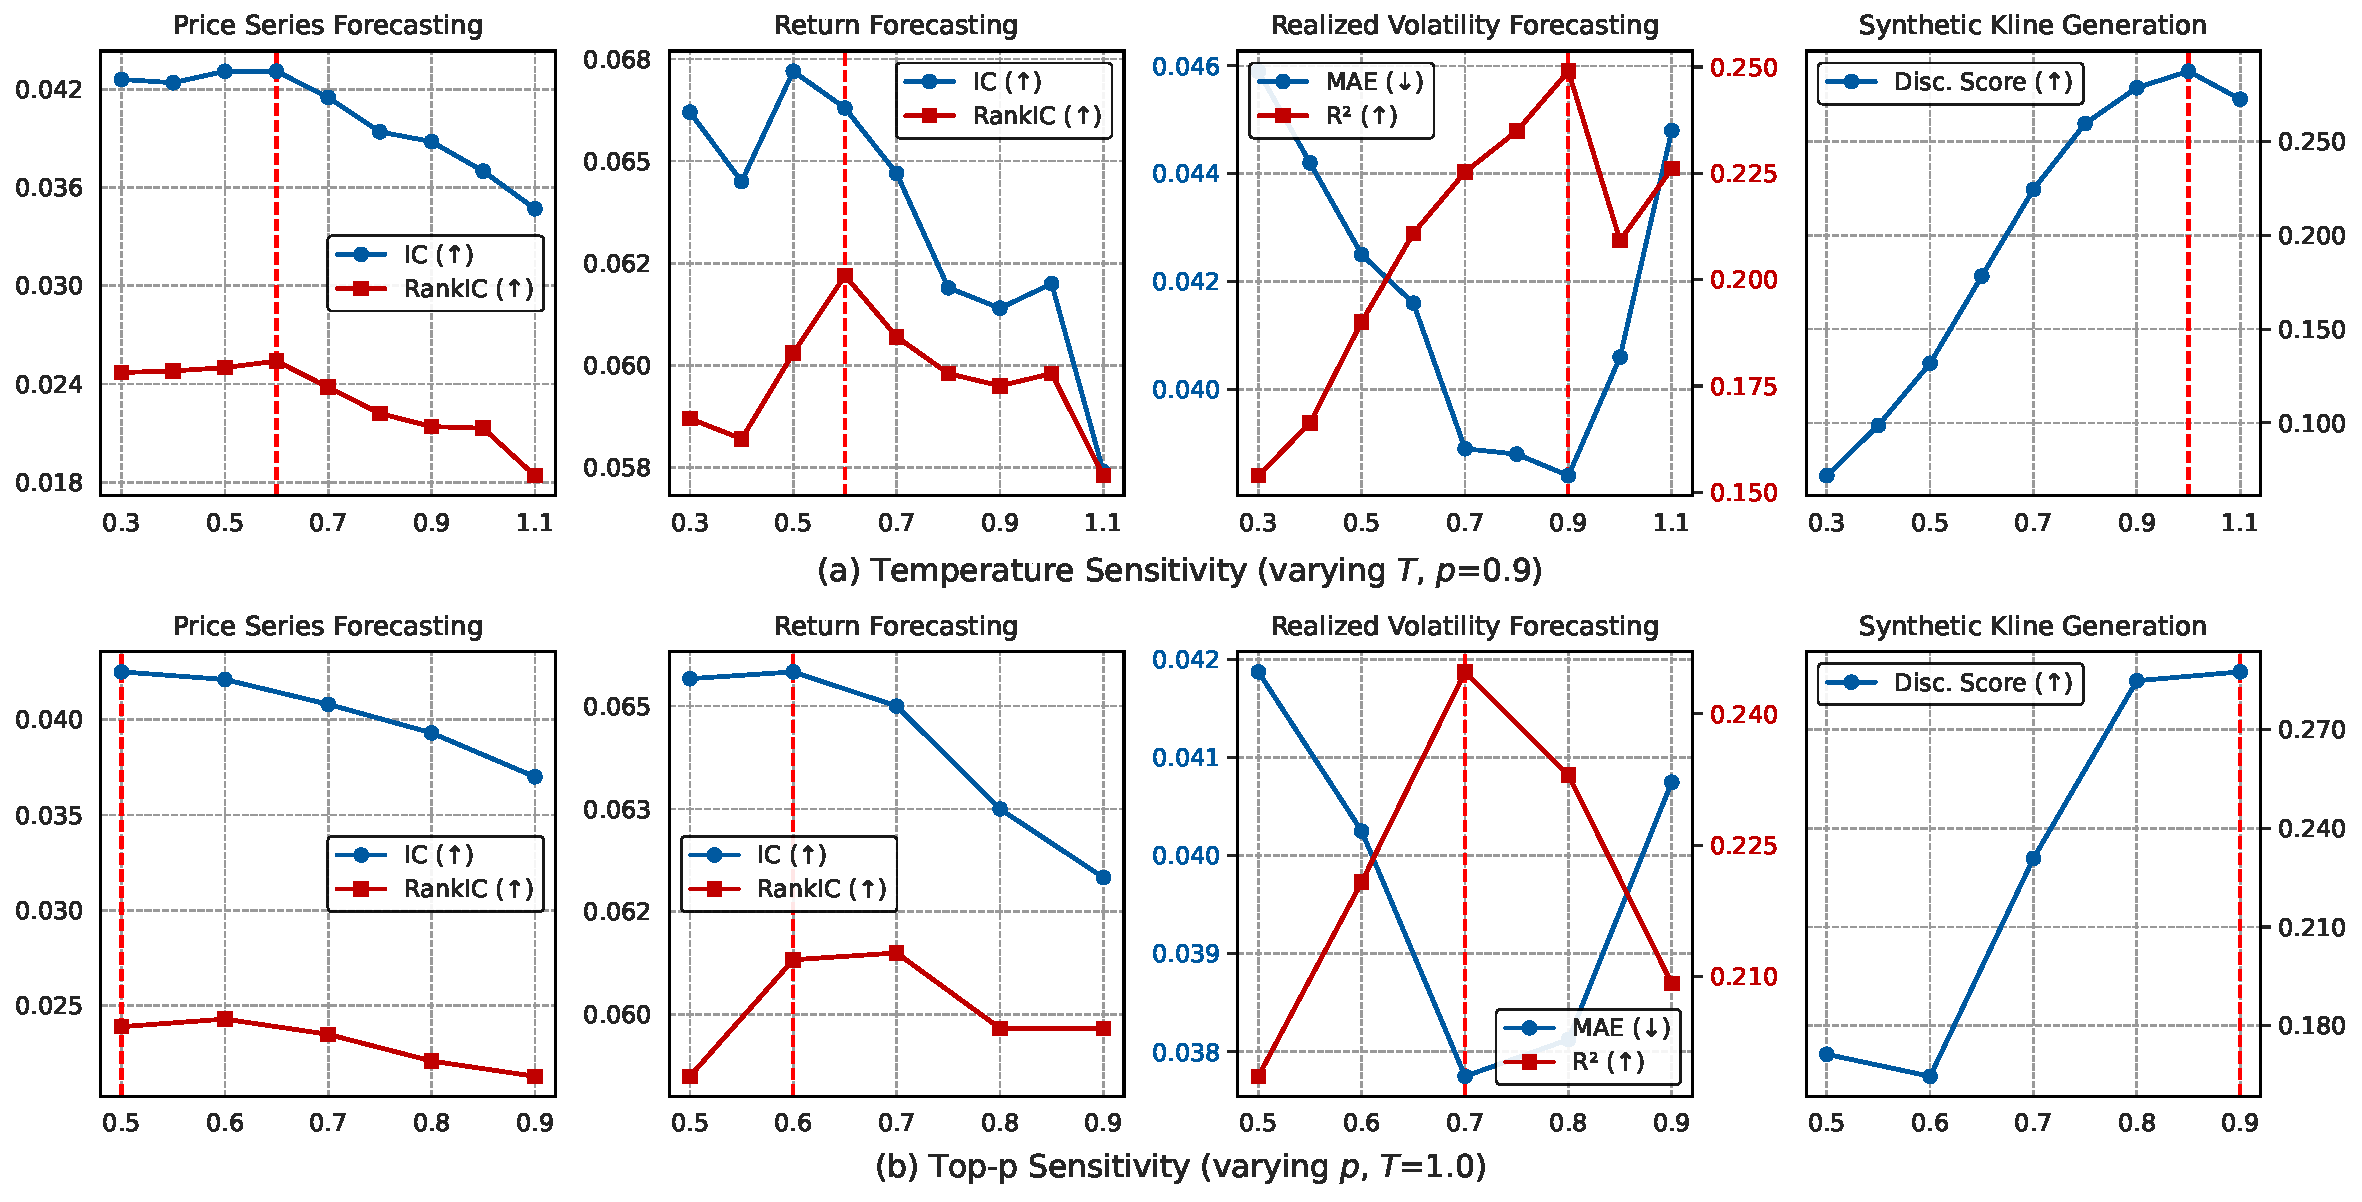
\includegraphics[width=1.0\textwidth]{img/sample_T_and_top_p_ablation.pdf}
    \caption{Sensitivity analysis of Kronos's performance on downstream tasks with respect to inference sampling hyperparameters. (a) Varying temperature $T$ while keeping top-$p=0.9$ fixed. (b) Varying top-$p$ while keeping temperature $T=1.0$ fixed. Optimal values, indicated by red dashed lines, are task-dependent, highlighting different requirements for precision versus diversity.}
    \label{fig:T_and_top_p}
\end{figure*}

\subparagraph{데이터셋과 생성 파라미터} We use data from two stock exchanges (in-distribution XSHG and out-of-distribution XTAI), as well as the cryptocurrency and forex datasets. We evaluate generation on two frequencies: 15-minute and daily. For the 15-minute frequency, we use a look-back window of 120 and generate a future sequence of length 96. For the daily frequency, the look-back is 96 and the generation horizon is 35. For each asset-frequency pair, we generate 6,000 synthetic sequences for evaluation.

\subparagraph{평가 지표}
\begin{itemize}
    \item \textbf{Discriminative Score:} To assess the fidelity of the generated data, we employ a post-hoc LSTM-based classifier to distinguish between real and synthetic sequences. The classifier consists of a single LSTM layer with a hidden dimension of 32. For training, we construct a balanced dataset of 6,000 samples (3,000 real, 3,000 synthetic) and a held-out test set of the same size and composition. The model is trained for 20 epochs with a batch size of 64, using the Adam optimizer (learning rate = 0.0005) and the binary cross-entropy (BCE) loss function. The Discriminative Score is defined as the classification error on the test set. A score approaching 0.5 indicates higher fidelity, signifying that the classifier struggles to differentiate generated data from real data.

    \item \textbf{Usefulness (TSTR):} To measure the practical usefulness of the synthetic data, we adopt the Train-on-Synthetic, Test-on-Real (TSTR) methodology. We train a post-hoc LSTM prediction model to forecast a future K-timestep window given a historical one. This model comprises two LSTM layers with a hidden dimension of 64. It is trained exclusively on 6,000 generated synthetic sequences for 20 epochs using the Adam optimizer (learning rate = 0.001) and a batch size of 64, with the Mean Squared Error (MSE) loss as the objective function. The look-back and horizon windows are set to (80, 16) for 15-minute data and (30, 5) for daily data, respectively. The trained model is then evaluated on the original, real test data. The final usefulness score is reported as the average Information Coefficient (IC) and Rank Information Coefficient (RankIC) of the predicted price series.
\end{itemize}

\paragraph{투자 시뮬레이션 설정}

To evaluate the practical profitability of Kronos and other baselines in real-world markets, we conduct an investment simulation on the Chinese A-share market. For simplicity, regarding the Zero-shot Time Series Models, we only select the largest-sized model from each family for comparison.

\subparagraph{데이터} Our empirical analysis utilizes daily market data for the Chinese A-share market, sourced from the Qlib platform~\cite{yang2020qlib}, an open-source framework for quantitative finance. To promote transparency and reproducibility, we apply no additional filtering or preprocessing to the data, using it in its original, unprocessed state. Furthermore, we conduct all backtesting simulations within the Qlib framework. This approach leverages its integrated backtesting engine to ensure a standardized and consistent evaluation protocol for all models under review.

\subparagraph{전략} We employ the top-$k$/drop-$n$ portfolio construction strategy. On each trading day, all stocks in the investment universe are ranked based on their predicted return signal. An equal-weight portfolio is formed by taking long positions in the top $k$ stocks. To manage turnover and trading costs, a maximum of $n$ stocks are bought or sold daily, and a minimum holding period of 5 days is enforced for all positions.

\subparagraph{신호와 백테스트}

The predictive signal is formulated as an expected return derived from a multi-step price forecast over a horizon of $H$ days. This signal generation pipeline is applied uniformly to all models under evaluation, including Kronos and the baselines, to ensure a fair comparison. For any given stock on trading day $t$, a sequence of forecasted closing prices for the subsequent $H$ days, denoted as $\{\hat{p}_{t+i}\}_{i=1}^{H}$, is first generated by the respective model. The signal, which we term the $H$-day average expected return ($R_{t \to t+H}$), is then calculated by comparing the arithmetic mean of these forecasted prices to the current closing price $p_t$:
\begin{equation}
R_{t \to t+H} = \frac{\left(\frac{1}{H}\sum_{i=1}^{H} \hat{p}_{t+i}\right) - p_t}{p_t}
\end{equation}
In our experiments, we set the forecast horizon to $H=10$. All price forecasts are generated using daily K-line data with a 90-day look-back window. This methodology is designed to produce a robust signal by averaging the forecasted price path, thereby mitigating the influence of short-term prediction noise and capturing the underlying trend more effectively.

Backtests are performed on the constituents of the CSI 300 and CSI 800 indices. These indices are chosen as they represent two key segments of the Chinese A-share market: the CSI 300 comprises large-cap, highly liquid stocks, while the CSI 800 provides broader market coverage by including both large- and mid-cap stocks. This allows for a comprehensive assessment of the model's performance across different market segments.


\subparagraph{파라미터와 비용} For the CSI 300 index, we set $k=50$ and $n=5$. For the broader CSI 800 index, we set $k=200$ and $n=10$. The relatively large portfolio sizes are chosen to ensure diversification and produce more stable backtesting results, reducing the influence of idiosyncratic stock movements. To ensure a realistic performance assessment, a conservative transaction cost of 0.15\% is applied to each trade.

\begin{figure*}[t!]
    \centering
    \begin{minipage}[t]{1.0\columnwidth}
        \centering
        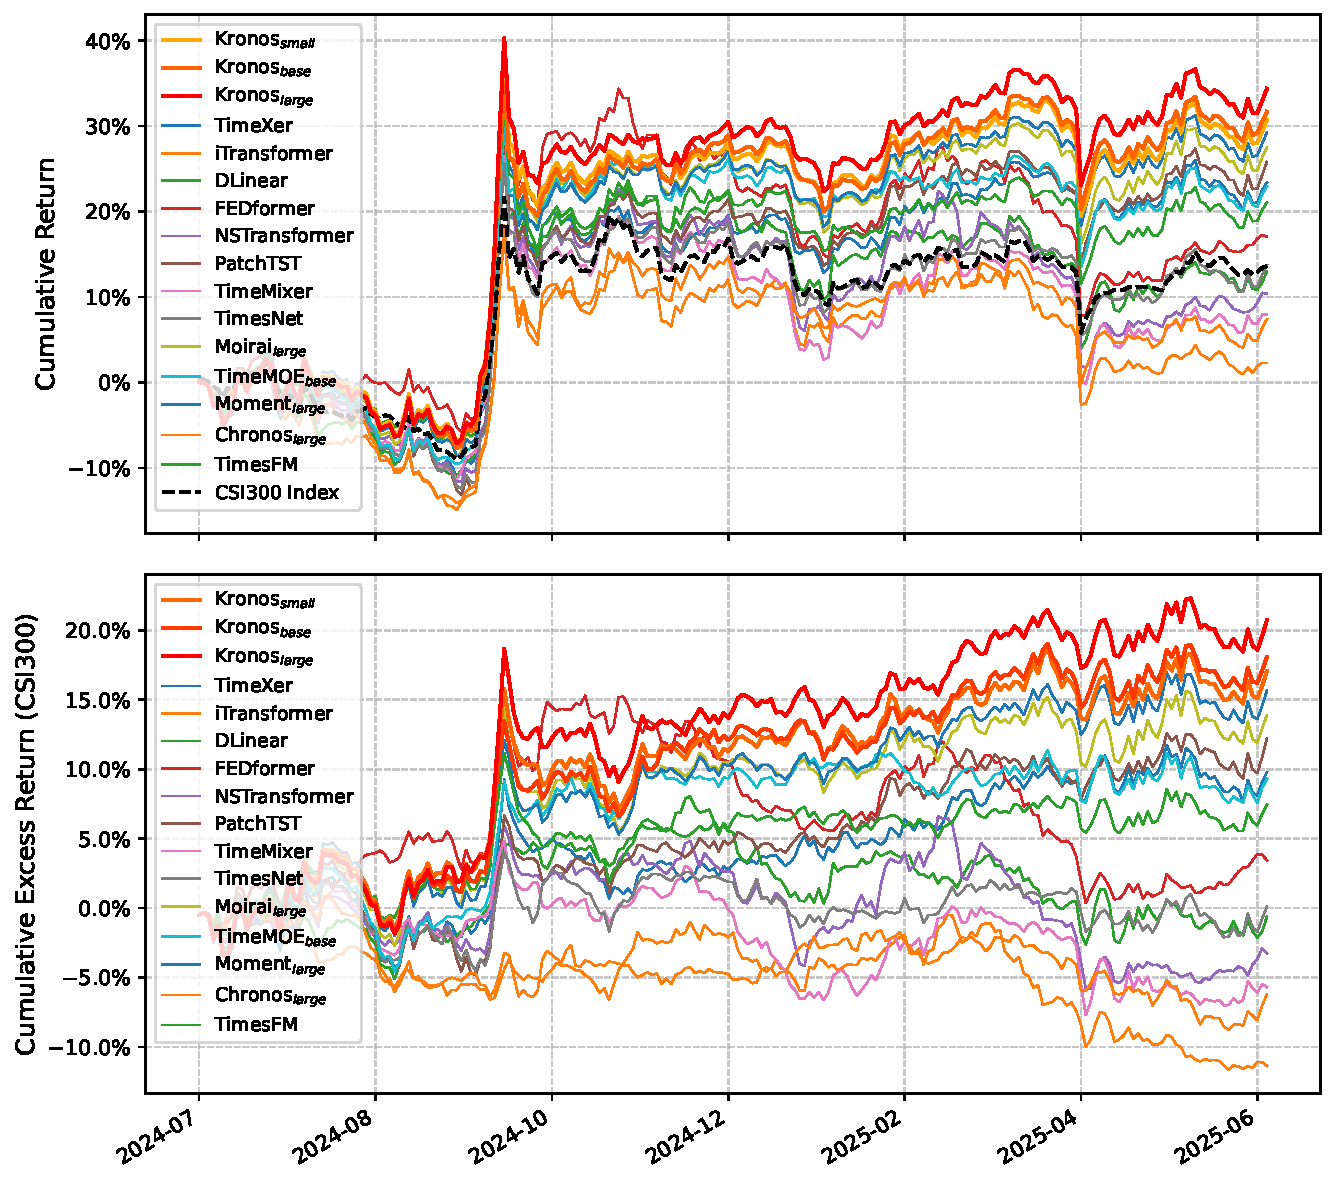
\includegraphics[width=\columnwidth]{img/backtest_csi300.pdf}
        \caption*{ (a) CSI300 Index}
    \end{minipage}
    \hspace{0.02\columnwidth}
    \begin{minipage}[t]{1.0\columnwidth}
        \centering
        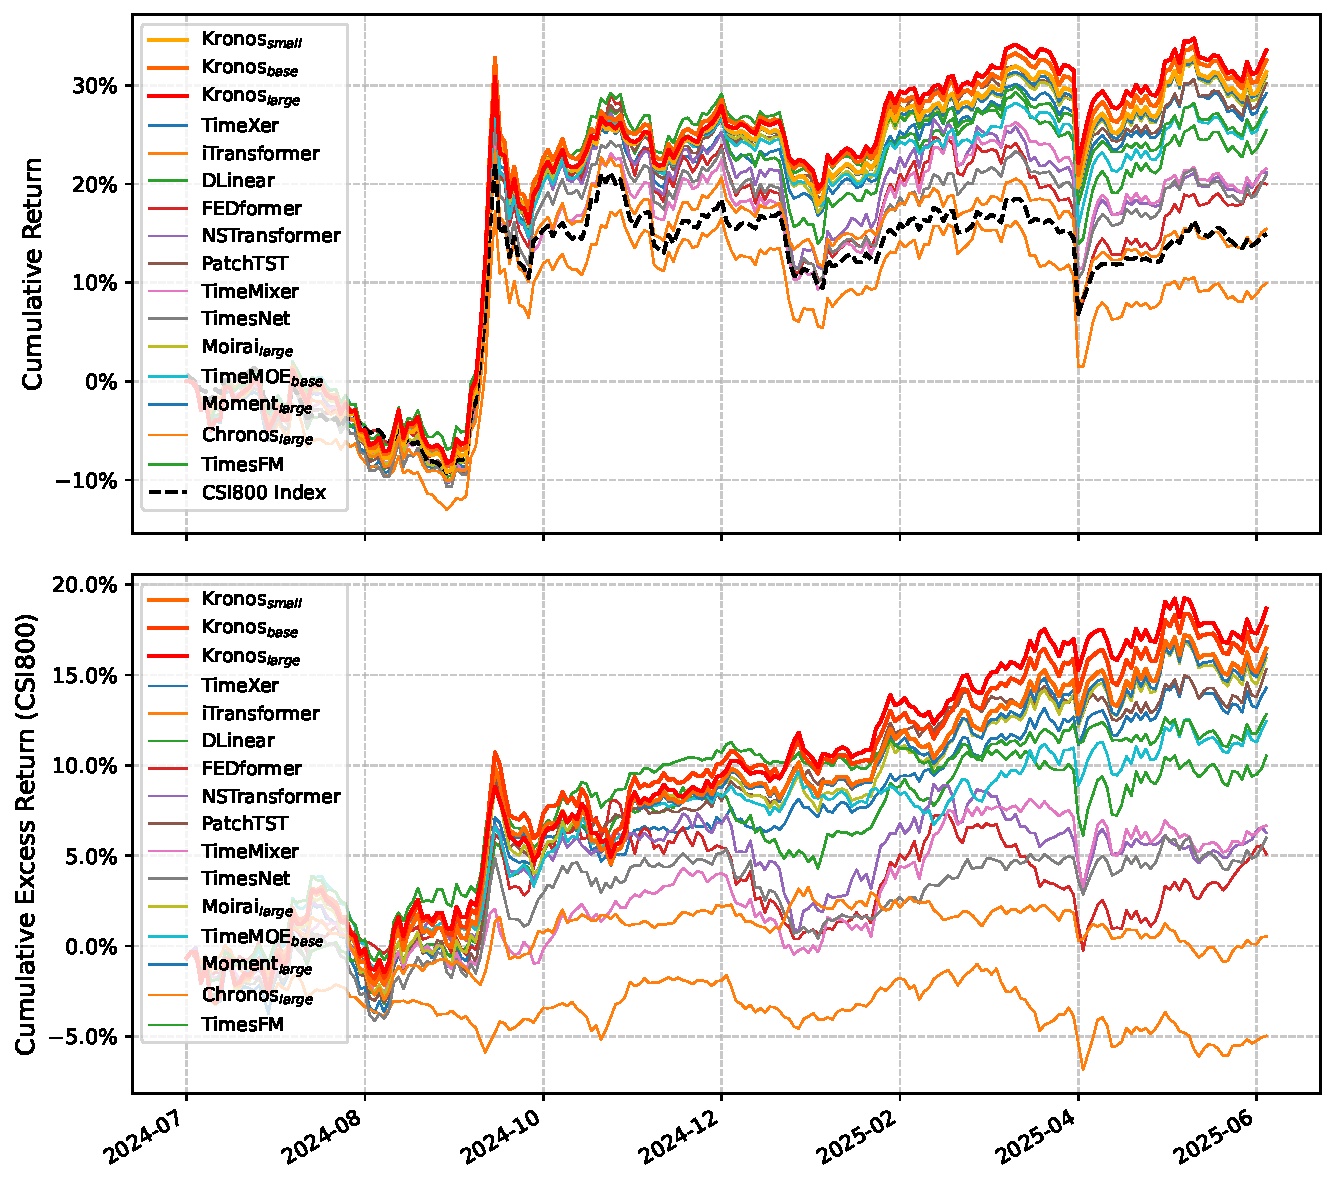
\includegraphics[width=\columnwidth]{img/backtest_csi800.pdf}
        \caption*{ (b) CSI800 Index}
    \end{minipage}
    \caption{서로 다른 모델이 생성한 신호를 사용한 백테스트의 누적 수익률 곡선.}
    \label{fig:backtest_profit}
\end{figure*}

\subsection{제거 연구 베이스라인 세부 사항}
\label{sec:ablation_baselines}

To investigate the architectural choices of Kronos, we design three baseline variants for our ablation study (Table~\ref{tab:ablation_study_refined}). Each variant targets a different modeling paradigm, allowing us to isolate the benefits of our proposed discrete, sequential framework. Below we provide a detailed description of each model.

\noindent\textbf{Direct-AR.} This model serves as a standard autoregressive forecasting baseline in the continuous space. Given a sequence of input features $\{x_1, \dots, x_T\}$, each feature vector $x_t \in \mathbb{R}^D$ is first mapped to a higher-dimensional embedding via a linear projection. The sequence of embeddings is then processed by a Transformer decoder backbone. The model is trained to directly predict the value of the next time step, $\hat{x}_{T+1}$, from the historical context. The training objective is to minimize the Mean Squared Error (MSE) between the predicted and ground-truth values. This approach represents the most common regression-based formulation for time series forecasting.

\noindent\textbf{Prob-AR.} This is a probabilistic forecasting model operating in the continuous space. Following established practices~\cite{yao2024towards}, instead of a point estimate, Prob-AR predicts the parameters of a probability distribution for the next time step. We use a mixture of four Student-t distributions to model the predicted distribution. The probability density function (PDF) for a random variable $x$ following a single Student-t distribution is:
\begin{equation}
p(x | \nu, \mu, \sigma) = \frac{\Gamma(\frac{\nu+1}{2})}{\Gamma(\frac{\nu}{2})\sqrt{\pi\nu}\sigma} \left(1 + \frac{1}{\nu}\left(\frac{x-\mu}{\sigma}\right)^2\right)^{-\frac{\nu+1}{2}}
\end{equation}
where $\nu > 0$, $\mu \in \mathbb{R}$, and $\sigma > 0$ are the degrees of freedom, location, and scale parameters, respectively, and $\Gamma(\cdot)$ is the gamma function. The model employs independent linear layers to predict the parameters for each of the four components—degrees of freedom ($\nu_k$), location ($\mu_k$), scale ($\sigma_k$), and mixture weights ($w_k$). To ensure parameter validity, a softplus transformation is applied to $\nu_k$ and $\sigma_k$ to enforce positivity, and a softmax function is applied to the weights $w_k$ to ensure they form a valid probability distribution. The model is trained by minimizing the Negative Log-Likelihood (NLL) of the true value under the predicted mixture distribution.

\noindent\textbf{Kronos-Parallel.} This variant is a direct ablation of the sequential subtoken generation mechanism within Kronos. While it shares the same input quantization and discrete prediction space as Kronos, it removes the intra-block module. After the Transformer backbone produces a context vector from the input history, a single prediction head is used to concurrently predict the logits for both subtokens of the next time step. The training objective is the sum of the cross-entropy losses for each subtoken, optimized jointly.

\subsection{실험 환경}
\label{sec:exp_environment}

All experiments are conducted within a Kubernetes (k8s) cluster. For all computational tasks, we utilize three identical pods. Each pod is provisioned with a dedicated set of resources comprising 96 CPU cores (Intel Xeon Gold 6330 @ 2.00 GHz), 200 GB of system memory (RAM), and eight NVIDIA GeForce RTX 4090D GPUs. This configuration provides a total of 24 GPUs, which are collectively employed for model training and all subsequent evaluations.

The software environment is containerized and standardized across all pods. The primary components and their versions are detailed below:
\begin{itemize}
    \item \textbf{Operating System:} Ubuntu 24.04.1 LTS
    \item \textbf{Software versions:} Python 3.13.2, PyTorch 2.7.0, NumPy 1.26.2, Pandas 2.2.2, Matplotlib 3.9.3, Hugging Face Hub (`huggingface\_hub') 1.57.4
\end{itemize}


\section{추가 결과}

\subsection{추론 샘플링 하이퍼파라미터의 영향}
\label{sec:sampling_hyperparams}

The autoregressive generation process of Kronos is governed by sampling strategies that introduce controlled stochasticity, namely temperature scaling ($T$) and top-$p$ (nucleus) sampling. The choice of these hyperparameters can significantly influence model performance on different downstream tasks. To provide guidance on their optimal settings, we conduct a sensitivity analysis. Figure~\ref{fig:T_and_top_p} illustrates the performance of Kronos across our four main tasks while varying one hyperparameter and holding the other constant.

As shown in Figure~\ref{fig:T_and_top_p}, the optimal sampling hyperparameters are task-dependent. For forecasting tasks (price series and return), which demand precision, lower temperatures (e.g., $T \approx 0.6$) are preferable. This sharpens the next-token distribution, compelling the model towards more deterministic and high-confidence predictions. Conversely, realized volatility forecasting and synthetic K-line generation benefit from greater stochasticity, achieving optimal performance at temperatures closer to 1.0. A higher temperature encourages the generation of more diverse sequences, which is essential for capturing the probabilistic nature of volatility and for producing realistic, non-repetitive market data.

The analysis of top-$p$ sampling reveals a similar pattern: forecasting tasks favor smaller $p$ values to restrict the sampling pool, whereas generative tasks perform better with a larger nucleus ($p \ge 0.9$) to preserve diversity. When comparing the two techniques, we observe that temperature scaling generally offers more effective and nuanced control, leading to slightly better peak performance across tasks. This suggests that the global probability rescaling of temperature may be a more suitable tuning mechanism than the hard truncation of nucleus sampling.

\subsection{토크나이저 아키텍처 제거 연구}
\label{sec:tokenizer_ablation}
We perform an ablation study on the tokenizer architecture to justify our design choices. We compare our proposed Transformer-based tokenizer using a hierarchical loss against two alternatives: (1) a Transformer-based tokenizer with a standard, non-hierarchical reconstruction loss and (2) a CNN-based architecture with a comparable parameter count. All models are trained with a vocabulary size of $2^{18}$.

\begin{table}[ht]
\centering

\resizebox{\columnwidth}{!}{%
\begin{tabular}{@{}l S[table-format=1.4] S[table-format=1.4]@{}}
\toprule
\textbf{토크나이저 아키텍처} & {\textbf{MAE} ($\downarrow$)} & {\textbf{MSE} ($\downarrow$)} \\
\midrule
\textbf{Transformer w/ Hierarchical Loss (Ours)} & 0.0785 & 0.0203 \\
Transformer w/ Standard Loss                   & 0.0781 & 0.0202 \\
\midrule
CNN-based                                      & 0.0916 & 0.0251 \\
\bottomrule
\end{tabular}%
}
\caption{
    Ablation study on the K-line tokenizer architecture. We compare our proposed Transformer-based tokenizer, which employs a hierarchical reconstruction loss, against two key variants: a Transformer-based tokenizer with a standard reconstruction loss and a CNN-based architecture. All models are trained with a vocabulary size of $2^{18}$. The table reports reconstruction quality measured by MAE and MSE.
}
\label{tab:tokenizer_ablation}
\end{table}

As shown in Table~\ref{tab:tokenizer_ablation}, the results indicate that Transformer-based architectures outperform the CNN-based model in reconstruction quality, highlighting the effectiveness of self-attention for capturing dependencies in K-line data. More importantly, our model with hierarchical loss achieves reconstruction quality nearly identical to that of the standard loss variant. This confirms that our approach successfully engineers a coarse-to-fine structure within the tokens—a property beneficial for the subsequent autoregressive model—without a notable trade-off in representational fidelity.

\subsection{K-line 재구성 시각화}

Figure~\ref{fig:recon_case} visualizes our tokenizer's reconstruction results on a diverse set of financial instruments. The plots show that the reconstructed `Close Price' and `Volume' series closely track the ground truth, confirming that our tokenizer effectively preserves the essential dynamics of the original continuous data within its discrete token representation.
% We note that due to the clipping of normalized input values to the range $[-5, 5]$ (see Appendix~\ref{sec:input_processing}), the tokenizer does not fully capture extreme outliers. This is a deliberate trade-off, as we find it enhances training stability and ultimately improves the generation quality of the subsequent autoregressive model.

\subsection{누적 수익률 곡선 시각화}

Figure~\ref{fig:backtest_profit} presents the cumulative return curves derived from backtesting using predictive signals by different models. As illustrated, Kronos consistently demonstrates superior performance, achieving the highest cumulative returns among the evaluated models.

\begin{table}[t]
  \centering
  \footnotesize
  \setlength{\tabcolsep}{4pt}

  \adjustbox{max width=\columnwidth}{
  \begin{tabular}{l *{6}{S}}
    \toprule
    \multirow{2}{*}{\textbf{Model}} & \multicolumn{2}{c}{\textbf{CSI300 Index}} & \multicolumn{2}{c}{\textbf{CSI800 Index}} & \multicolumn{2}{c}{\textbf{Average}} \\

    \cmidrule(lr){2-3} \cmidrule(lr){4-5} \cmidrule(lr){6-7}

    & \textbf{AER} & \textbf{IR} & \textbf{AER} & \textbf{IR} & \textbf{AER} & \textbf{IR} \\
    \midrule

    TimeXer       & 0.1035 & 0.7988 & 0.1509 & 1.5471 & 0.1272 & 1.1730 \\
    TimeMixer       & -0.0600 & -0.5721 & 0.0705 & 0.8113 & 0.0053 & 0.1196 \\
    iTransformer       & -0.1202 & -1.4441 & -0.0525 & -0.8558 & -0.0864 & -1.1500 \\
    PatchTST       & 0.1289 & 0.9895 & 0.1620 & 1.5033 & 0.1455 & 1.2464 \\
    TimesNet       & 0.1441 & 0.6558 & 0.0634 & 0.7225 & 0.1038 & 0.6892 \\
    DLinear       & -0.0066 & -0.0605 & 0.1112 & 1.2003 & 0.0523 & 0.5699 \\
    FEDformer       & 0.0362 & 0.2943 & 0.0539 & 0.5602 & 0.0451 & 0.4273 \\
    NSTransformer       & -0.0343 & -0.2889 & 0.0664 & 0.6979 & 0.0161 & 0.2045 \\

    \midrule

    $\text{Time-MOE}_{base}$       & 0.0985 & 0.8230 & 0.1315 & 1.3726 & 0.1150 & 1.0978 \\
    $\text{Moirai}_{large}$       & 0.1470 & 0.9747 & 0.1683 & 1.5215 & 0.1577 & 1.2481 \\
    TimesFM       & 0.0788 & 0.7357 & 0.1355 & 1.6427 & 0.1072 & 1.1892 \\
    $\text{Moment}_{large}$       & 0.1655 & 1.1993 & 0.1707 & 1.5361 & 0.1681 & 1.3677 \\
    $\text{Chronos}_{large}$       & -0.0659 & -0.7670 & 0.0056 & 0.0902 & -0.0302 & -0.3384 \\

    \midrule
    \textbf{$\text{Kronos}_{small}$} & 0.1805 & 1.2394 & 0.1772 & 1.6050 & 0.1789 & 1.4222 \\
    \textbf{$\text{Kronos}_{base}$} & \second{0.1911} & \second{1.3782} & \second{0.1867} & \second{1.6652} & \second{0.1889} & \second{1.5217} \\
    \textbf{$\text{Kronos}_{large}$} & \best{0.2193} & \best{1.4177} & \best{0.1974} & \best{1.8805} & \best{0.2084} & \best{1.6491}\\
    \bottomrule
  \end{tabular}}
  \caption{Full results of investment simulation. We report Annualized Excess Return (AER) and Information Ratio (IR). Best and second best results are marked with \best{red underline} and \second{blue underline}, respectively.
  }
  \label{tab:full_backtest_result}
\end{table}

\section{전체 실험 결과}
\label{sec:full_exp_results}

In this section, we present the complete experimental results for three forecasting tasks and the synthetic K-line generation task. For the forecasting tasks, we report the results for each asset, averaged over all tested frequencies.
Tables~\ref{tab:full_price_forecasting_1} and~\ref{tab:full_price_forecasting_2} show the results of the price series forecasting experiments.
The outcomes for return forecasting are presented in Tables~\ref{tab:full_return_forecasting_1} and~\ref{tab:full_return_forecasting_2}, while those for realized volatility forecasting are in Tables~\ref{tab:full_volatility_forecasting_1} and~\ref{tab:full_volatility_forecasting_2}.
Furthermore, for the synthetic K-line generation task, Figures~\ref{fig:gen_visual_1} and~\ref{fig:gen_visual_2} provide visualizations of the \textit{diversity} of the generated sequences by different models. The results for the discriminative score and predictive usefulness are presented in Table~\ref{tab:generate_discriminative} and Table~\ref{tab:generate_usefulness}, respectively. Finally, the results of the investment simulation experiment are presented in Table~\ref{tab:full_backtest_result}.

\section{예측 사례}

Figures~\ref{fig:pred_case_1} to \ref{fig:pred_case_5} present the forecasting results of our proposed model, Kronos, against several baselines.
We select a few representative assets and showcase the predictions for two key features: closing price and trading volume.
As observed, the forecasts from Kronos not only achieve competitive predictive performance but also exhibit a strong qualitative resemblance to the ground-truth series.
Notably, our model adeptly captures the characteristic dynamics and patterns of the actual price and volume sequences, producing forecasts that are not only accurate but also visually plausible.

\section{논의}
\label{sec:discussion}


\subsection{K-line 데이터는 단기 자본시장 가격 움직임을 이끌 충분한 정보를 내포하는가? (Q1)}

% In capital markets, the factors driving price movements can be broadly categorized into two types: short-term factors, which are highly volatile and have immediate effects, and long-term factors, which exhibit clear trends and have a profound impact on value formation.

% Long-term factors determine the overall direction and valuation level of the market, while short-term factors generate volatility and trading opportunities.

% A large number of empirical research shows that price and trading volume together can reflect the information embedded in short-term drivers such as macroeconomic announcements, corporate events, and market sentiment.

In capital markets, the determinants of price dynamics are conventionally bifurcated into:

\begin{itemize}
\item \textbf{Long‐term driving factors}, which manifest as persistent trends and exert a lasting influence on intrinsic value;
\item \textbf{Short‐term driving factors}, which are typified by elevated volatility and immediate market impact.

\end{itemize}

Long‐term driving factors establish the market’s prevailing trajectory and valuation benchmarks, whereas short‐term ones introduce transient volatility and generate discrete trading opportunities.

Extensive empirical evidence demonstrates that kline data (\textbf{OHLCVA}, including \textbf{price} and \textbf{trading volume})~\cite{kim1991trading}, when analyzed in tandem, effectively encapsulate the informational content of short‐term driving factors—such as macroeconomic data releases ~\cite{flannery2002macroeconomic}, corporate event disclosures~\cite{kim1991trading}, and shifts in investor sentiment~\cite{baker2006investor, da2011search}.



The detail discussion about the above empirical evidences is beyond the scope of this paper.


% \subsection{Kronos의 토크나이저가 작동하는 이유는 무엇인가? (Q2)}

% The motivation for using vision‑inspired quantization (BSQ) in time-series modeling could be discussed from the perspectives of artificial intelligence model and financial market micro-structure.

% \subsubsection{Noise suppression and stability}

% % High‑frequency K‑line bars (e.g., 5‑minute or 15‑minute intervals) often contain a lot of  noises (like quote flickers and small outlier trades). BSQ reduces these noises by first mapping each continuous feature vector onto a fixed set of points on a sphere and then converting it to a binary token. The outcome is a steadier ``token sequence'' that filters out those fleeting blips and instead highlights genuine shifts in the market’s structure (for example, market trends, regime changes or sudden liquidity sweeps).

% Using quantization to transform regression into classification-style problems could improve the stability and reliability of financial forecasting models.

% Additionally, by projecting embeddings onto the unit sphere before binarizing, BSQ~\cite{zhao2024image} guarantees
%     \[
%       \mathbb{E}_u \,\big\|u - \widehat u\big\|\;<\;\sqrt{2 - 2/\sqrt{L}}\;<\sqrt{2},
%     \]
% so the distortion is strictly upper‑bounded and shrinks as the codebook dimension \(L\) grows.
% In contrast, the sign-based quantization without normalization (LFQ) has unbounded error.


% In financial markets, there are outliers—for example, a “flash‑crash” data point caused by an anomalous trade match in liquidity shortage. The bounded quantization error prevents extreme outlier values from producing arbitrarily large approximation errors.


% \subsubsection{Compact, discrete state space}
% Discretizing into a small set of binary codes transforms high‑dimensional price‐volume vectors into a compact token sequence. This drastically reduces the vocabulary size for downstream sequence models, improving sample efficiency and reducing overfitting—especially critical when modeling rare quotes under various shocks.


% \begin{table}[th]
% \centering
% \sisetup{table-format=1.4}
% \begin{tabular*}{\columnwidth}{@{\extracolsep{\fill}} l S S}
% \toprule
% \textbf{Dataset} & {\textbf{MAE}} & {\textbf{MSE}} \\
% \midrule
% XHKG     & 0.0798 & 0.0201 \\
% XIDX     & 0.0903 & 0.0265 \\
% XJPX     & 0.0776 & 0.0207 \\
% XKLS     & 0.0871 & 0.0220 \\
% XKRX     & 0.0849 & 0.0236 \\
% XNAS     & 0.0836 & 0.0223 \\
% XNSE     & 0.0805 & 0.0208 \\
% XSHG     & 0.0755 & 0.0148 \\
% XTAI     & 0.0785 & 0.0195 \\
% Crypto   & 0.0417 & 0.0044 \\
% Forex    & 0.0541 & 0.0081 \\
% \midrule
% \textbf{Average} & \bfseries 0.0770 & \bfseries 0.0192 \\
% \bottomrule
% \end{tabular*}
% \caption{
% Reconstruction performance of different datasets.(The full names of \textit{Dataset} colume can be found in Appendix~\ref{sec:exp_setup_details} section \textit{Forecasting Task Setup}.)
% }
% \label{tab:reconstruction_performance}
% \end{table}


% As is shown in Table \ref{tab:codebook_usage}, the code usage of BSQ reaches 97.66\% at the coarse level and 85.25\% at the fine level in Krono's tokenizer, which contributes to a more nuanced representation of market microstructure.


\subsection{Kronos의 토크나이저가 작동하는 이유는 무엇인가? (Q2)}

The effectiveness of our vision-inspired quantization (BSQ) tokenizer can be analyzed from two key perspectives: its inherent noise suppression and its ability to create a structured, discrete state space suitable for sequence modeling.

\subsubsection{노이즈 억제와 안정성}
Financial time-series data is often corrupted by noise and subject to extreme outliers, such as ``flash-crash'' events caused by anomalous trades. A primary challenge for regression-based models is that such outliers can lead to unbounded approximation errors, severely degrading model stability~\cite{brownlees2006financial}.

Our approach addresses this by transforming the representation learning into a more robust, classification-like framework. By quantizing continuous price-volume embeddings, we effectively cap the influence of any single data point. Specifically, BSQ's projection of embeddings onto a unit sphere prior to binarization guarantees that the expected distortion is strictly upper-bounded~\cite{zhao2024image}:
\[
  \mathbb{E}_u \,\big\|u - \widehat u\big\|\;<\;\sqrt{2 - 2/\sqrt{L}}\;<\sqrt{2}.
\]
This bound tightens as the codebook dimension \(L\) increases. In contrast, simpler methods like sign-based quantization without normalization (e.g., LFQ) lack such a guarantee, leaving them vulnerable to arbitrarily large errors from outlier inputs~\cite{zhao2024image}. This bounded error property is crucial for building reliable financial forecasting models.

\subsubsection{작고 이산적인 상태 공간에서의 학습}
High-frequency financial data exists in a high-dimensional, continuous state space, posing significant challenges for sequence models. Our tokenizer maps these infinite states into a finite, discrete vocabulary of tokens. This discretization serves as a powerful form of regularization with two main benefits~\cite{rabanser2020effectiveness}:

\begin{itemize}
    \item \textbf{Improved Sample Efficiency and Generalization}: Instead of learning a complex function over a continuous space, a downstream model like a Transformer learns to predict transitions and patterns among a finite set of abstract states (tokens). This simplifies the learning task. Different but semantically similar input vectors can be mapped to the same token, effectively increasing the number of observations for each discrete state. This allows the model to learn robust patterns from fewer examples, which is particularly critical for modeling rare market phenomena like responses to liquidity shocks, where data is sparse.
    \item \textbf{Reduced Overfitting}: The quantization process inherently discards fine-grained, potentially noisy variations within each quantization cell. This prevents the model from fitting to spurious artifacts in the training data.
\end{itemize}

\begin{table}[h!]
\centering

\resizebox{\columnwidth}{!}{%
\begin{tabular*}{\columnwidth}{@{\extracolsep{\fill}} ccc}
\toprule
\textbf{코드북 유형} & \textbf{크기} & \textbf{사용률} \\
\midrule
Coarse-Level-Subtoken Codebook      & $2^{10}$ & 97.66\% \\
Fine-Level-Subtoken Codebook        & $2^{10}$ & 85.25\% \\
\bottomrule
\end{tabular*}}

\caption{거친 수준 서브토큰과 세밀한 수준 서브토큰의 코드북 사용률.}
\label{tab:codebook_usage}
\end{table}

\begin{table*}[t!]
\centering

\resizebox{\textwidth}{!}{%
\begin{tabular}{@{}l c c r r r r c@{}}
\toprule
\textbf{설정} & \textbf{Splits ($n$)} & \textbf{Sub-Vocab ($2^{k/n}$)} & \textbf{코어 파라미터 (M)} & \textbf{어휘 파라미터 (M)} & \textbf{융합 파라미터 (M)} & \textbf{총 파라미터 (M)} & \textbf{토큰당 추론 단계} \\
\midrule
No Split & 1 & 1,048,576 & 97.5 & 1744.8 & 0.0 & 1842.3 & 1$\times$ \\
\textbf{Ours} & \textbf{2} & \textbf{1,024} & \textbf{97.5} & \textbf{3.4} & \textbf{1.4} & \textbf{102.3} & \textbf{2$\times$} \\
More Splits & 4 & 32 & 97.5 & 0.2 & 2.8 & 100.5 & 4$\times$ \\
& 5 & 16 & 97.5 & 0.1 & 3.5 & 101.1 & 5$\times$ \\
\bottomrule
\end{tabular}%
}
\caption{
    Trade-off analysis for factorizing a $k=20$ bit token into $n$ subtokens, based on the $\text{Kronos}_{base}$ architecture. The model's core Transformer blocks have $\approx$97.5M parameters.
}
\label{tab:factorization_analysis_revised}
\end{table*}

The effectiveness of our tokenizer is further evidenced by its codebook utilization. As shown in Table \ref{tab:codebook_usage}, the code usage of BSQ reaches 97.66\% at the coarse level and 85.25\% at the fine level. Such high utilization indicates that our method creates an expressive vocabulary, effectively partitioning the feature space without suffering from codebook collapse (where many codes are left unused)~\cite{zhu2024addressing}. This expressiveness provides the rich foundation necessary for a model to capture the nuanced and diverse states of market microstructure.

% Table \ref{tab:reconstruction_performance} summarizes the reconstruction performance across different markets and asset classes, while Figure \ref{fig:recon_case} presents visualization examples of K-line reconstruction cases.

Additionally, the vocabulary is stratified into three categories based on usage frequency: (a) high-frequency, (b) low-frequency, and (c) unused tokens. To investigate their representational characteristics, we conduct an analysis where we replace the final token of an encoded sequence with a token from each category and then decode it back to a K-line. Figure \ref{fig:token_show_case} presents the results of this procedure. We observe a clear correspondence between token frequency and pattern typicality. High-frequency tokens (a) map to common K-bar shapes, indicative of stable market conditions. Conversely, low-frequency (b) and unused (c) tokens generate more extreme and atypical K-bars, such as those with long bodies or wicks, signifying rare, high-volatility events. This suggests that the learned codebook captures a meaningful semantic hierarchy, effectively distinguishing between common and significant market patterns based on token frequency.



\subsubsection{꼬리 민감성을 위한 초구면 기하}
In financial contexts, market returns and price changes often exhibit heavy tails (or fat tails)~\cite{mandelbrot1963variation}. The heavy-tail distribution of price changes is one of the key sources of trading profits in quantitative investment and cannot be ignored.

Unlike standard vector-quantization on the Euclidean sphere, BSQ’s binary encoding preserves angular information very efficiently, making it more sensitive to fat-tail data that manifest as sharp directional changes in feature space. This aligns well with how microstructure events often appear as abrupt shifts in the “direction” of the joint price-volume vector~\cite{podobnik2009cross}.

Figure~\ref{fig:kline_reconstruction_tradewar} illustrates the tokenizer's ability to capture and reconstruct the long-tailed market microstructure under short-term high volatility and during extreme gap events (in the economic context of Trump’s Trade War~\cite{mckibbin2025global}).

Above all, we summarize the concrete advantages of BSQ for K-line time series data, leveraging its ability to preserve angular information and capture sharp directional changes, which are crucial for modeling financial time series with heavy tails and abrupt shifts due to microstructure events.

\subsection{서브토큰 분해 분석 (Q3)}
\label{sec:subtoken_factorization}

Our methodology factorizes a $k$-bit token into $n$ subtokens to manage a large vocabulary size. A key design choice is the number of factors, $n$. While further factorization (e.g., $n>2$) could reduce sub-vocabulary sizes even more (e.g., from $2^{10}$ to $2^5$ for a $k=20$ token), we argue that $n=2$ offers the best trade-off between parameter efficiency and inference latency.

This factorization introduces a fundamental trade-off. On one hand, it significantly reduces the size of \textbf{vocabulary-dependent parameters} in the input embedding and output projection layers, replacing a single large table for a $2^k$ vocabulary with $n$ smaller tables for $2^{k/n}$ sub-vocabularies. On the other hand, it introduces two costs: (1) a new \textbf{fusion layer} ($W_{\text{fuse}}$ in Equation~\ref{eq:embedding}), whose parameters $(n \times \mathbf{d}_{\text{model}}) \times \mathbf{d}_{\text{model}}$ grow linearly with $n$, and (2) increased \textbf{inference latency}, as generating a full token requires $n$ sequential autoregressive steps.

Table~\ref{tab:factorization_analysis_revised} quantifies this trade-off for our $\text{Kronos}_{base}$ model. The most significant parameter reduction is achieved by moving from no factorization ($n=1$) to a 2-way split. This single step reduces vocabulary-dependent parameters by over 99.8\% (from $\approx$1.7B to 3.4M), shrinking the total model size by nearly 95\% and making a large effective vocabulary computationally feasible.

However, further factorization yields diminishing returns while incurring rising costs. Moving from $n=2$ to $n=4$ reduces vocabulary parameters by only 3.2M, a saving that is partially offset by a 1.4M increase in fusion layer parameters. This results in a marginal total parameter reduction of just $\approx$2\%. As $n$ increases to 5, the overhead from the fusion layer outweighs the savings from the smaller vocabularies, causing the total parameter count to increase. Crucially, these marginal or negative parameter benefits come at a direct and substantial latency cost: moving from $n=2$ to $n=4$ doubles the number of sequential generation steps required per token.

In summary, our choice of $n=2$ represents an effective balance. It captures the vast majority of the parameter-reduction benefits, making our large vocabulary practical, while avoiding the significant latency penalties and growing architectural overhead associated with finer-grained splits.


\onecolumn

\begin{footnotesize}
\begin{center}
\begin{longtable}{@{\extracolsep{\fill}} l l l r r l @{}}

    \toprule
    \textbf{거래소 / 국가} & \textbf{자산 유형} & \textbf{시간 주기} & \textbf{\# Assets} & \textbf{\# Observations} & \textbf{시작일} \\
    \midrule
    \endfirsthead
    \multicolumn{6}{c}%
    {{\bfseries\tablename\ \thetable{} -- Continued from previous page}} \\
    \toprule
    \textbf{거래소 / 국가} & \textbf{자산 유형} & \textbf{시간 주기} & \textbf{\# Assets} & \textbf{\# Observations} & \textbf{시작일} \\
    \midrule
    \endhead
    \midrule
    \multicolumn{6}{r@{}}{\textit{다음 페이지에 계속}} \\
    \endfoot

    \bottomrule \\
    \caption{다중 거래소, 다중 자산 K-line 데이터셋의 기술 통계. 시간 프레임 약어는 다음과 같다: T (1분), H (1시간), D (1일), W (1주).}
    \label{tab:dataset_overview} \\
    \endlastfoot

    Binance            & 암호화폐,무기한 스왑             & T, 5T, 15T, 30T, H, D, W        & 997   & 1,237,002,843   & 2021/1/31 \\
        Athens Stock Exchange          & 주식, ETF             & D, W        & 180   & 226,315   & 2023/4/11 \\
        Beijing Stock Exchange         & 주식       & 5T, 15T, 30T, H, D, W & 272      & 10,197,628   & 2021/11/19 \\
        Brazil Stock Exchange          & 주식, ETF       & D, W & 2,058      & 1,315,290   & 2020/1/31 \\
        Moscow Exchange             & 주식, ETF       & D, W              & 514     &  567,351    & 2020/1/31 \\
        Euronext Amsterdam             & 주식, ETF           & D, W                  & 514    & 602,083    & 2020/1/31 \\
        Australian Securities Exchange     & 주식, ETF           & 5T, 15T, 30T, H, D, W              & 3,381    & 86,613,897    & 2020/1/31 \\
        Stock Exchange of Thailand            & 주식, ETF        & 5T, 15T, 30T, H, D, W                  & 1,664   & 49,590,394    & 2020/1/31 \\
        Bombay Stock Exchange & 주식, ETF       & 5T, 15T, 30T, H, D, W              & 5,491 & 284,428,211 & 2020/1/31 \\
        Euronext Brussels & 주식, ETF       & D, W              & 166 & 195,491 & 2020/1/31 \\
        Bucharest Stock Exchange & 주식, ETF       & D, W  & 247 & 176,080 & 2020/1/31 \\
        Budapest Stock Exchange & 주식, ETF       & D, W  & 50 & 57,586 & 2022/1/14 \\
        Buenos Aires Stock Exchange & 주식 & D, W  & 183 & 225,352 & 2020/1/31 \\
        Colombo Stock Exchange & 주식 & D, W  & 292 & 372,627 &  2020/1/31 \\
        Copenhagen Stock Exchange & 주식 & D, W  & 825 & 617,464 & 2020/1/31 \\
        Frankfurt Stock Exchange & 주식, ETF & D, W  & 17,054 & 21,547,744 & 2020/1/31 \\
        Ghana Stock Exchange &  주식 & D, W  & 44 & 57,690 & 2020/1/31 \\
        Hong Kong Stock Exchange & 주식, ETF & 5T, 15T, 30T, H, D, W & 3,500 & 359,434,220  & 2020/1/31 \\
        Japan Exchange Group &  주식, ETF & 5T, 15T, 30T, H, D, W & 4,467 & 280,601,980 &  2020/1/31 \\
        Indonesia Stock Exchange & 주식 & 5T, 15T, 30T, H, D, W & 935 & 38,627,125 &  2020/1/31 \\
        Borsa Istanbul &  주식 & D, W  & 627 & 784,147 &  2020/1/31 \\
        Johannesburg Stock Exchange & 주식, ETF & D, W  & 562 & 681,587 & 2020/1/31 \\
        Pakistan Stock Exchange & 주식, ETF & D, W  & 660 & 595,505 & 2020/1/31 \\
        Kuala Lumpur Stock Exchange & 주식, ETF & 5T, 15T, 30T, H, D, W & 1,150 & 45,938,559 & 2020/1/31 \\
        Korea Exchange & 주식, ETF & 5T, 15T, 30T, H, D, W & 2,928 & 205,061,301 & 2020/1/31 \\
        Lima Stock Exchange & 주식, ETF & D, W  & 166 & 63,503 & 2020/1/31 \\
        Euronext Lisbon & 주식, ETF & D, W  & 60 & 65,753 & 2020/1/31 \\
        London Stock Exchange & 주식, ETF & 5T, 15T, 30T, H, D, W & 8,660 & 177,947,624 & 2020/1/31 \\
        Luxembourg Stock Exchange & 주식 & D, W  & 5 & 7,598 & 2020/1/31 \\
        Madrid Stock Exchange & 주식, ETF & D, W  & 309 & 331,745 & 2020/1/31 \\
        Mexican Stock Exchange & 주식, ETF & D, W  & 775 & 937,637 & 2020/1/31 \\
        Nasdaq Stock Exchange & 주식, ETF & T, 5T, 15T, 30T, H, D, W & 8,725 & 2,478,662,459 & 2000/1/1 \\
        National Stock Exchange of India & 주식, ETF & 5T, 15T, 30T, H, D, W & 2,554 & 242,429,169 & 2020/1/31 \\
        New York Stock Exchange & 주식, ETF & T, 5T, 15T, 30T, H, D, W & 7,073 & 2,133,143,549 & 2000/1/1 \\
        Euronext Paris & 주식, ETF & D, W  & 1,781 & 1,981,059 & 2020/1/31 \\
        Philippine Stock Exchange & 주식, ETF & 5T, 15T, 30T, H, D, W & 351 & 4,388,378 & 2020/1/31 \\
        Prague Stock Exchange & 주식 & D, W  & 50 & 62,666 & 2020/1/31 \\
        Santiago Stock Exchange & 주식 & D, W  & 225 & 160,638 & 2020/1/31 \\
        Shenzhen Stock Exchange & 주식, ETF & T, 5T, 15T, 30T, H, D, W & 3,519 & 1,754,519,331 & 1990/12/19 \\
        Shenzhen Stock Exchange (B-shares) & 주식 & 5T, 15T, 30T, H, D, W & 46 & 4,198,702 & 2020/2/3 \\
        Shanghai Stock Exchange & 주식, ETF & T, 5T, 15T, 30T, H, D, W & 3,064 & 1,967,996,343 & 1990/12/19 \\
        Shanghai Stock Exchange (B-shares) & 주식 & 5T, 15T, 30T, H, D, W & 50 & 4,526,152 & 2020/2/3 \\
        Stockholm Stock Exchange & 주식, ETF & D, W  & 1,305 & 1,463,722 & 2020/1/31 \\
        SIX Swiss Exchange & 주식, ETF & D, W  & 1,981 & 2,451,675 & 2020/1/31 \\
        Taiwan Stock Exchange & 주식, ETF & 5T, 15T, 30T, H, D, W & 1,252 & 71,619,260 & 2020/1/31 \\
        Toronto Stock Exchange & 주식, ETF & D, W  & 3,035 & 3,356,561 & 2020/1/31 \\
        Vienna Stock Exchange & 주식 & D, W  & 98 & 123,643 & 2020/1/31 \\
        중국 & 선물 & T, 5T, 15T, D & 75 & 63,318,960 & 2010/1/1 \\
        \textbackslash & 외환 & 5T, 15T, 30T, H, D, W & 1,023 & 462,434,562 & 2020/1/31 \\
        호주 & 주가지수 & 5T, 15T, 30T, H, D, W & 40 & 183,158 & 2020/1/31 \\
        벨기에 & 주가지수 & D, W  & 5 & 8,109 & 2020/1/31 \\
        브라질 & 주가지수 & D, W  & 3 & 4,766 & 2020/1/31 \\
        캐나다 & 주가지수 & D, W  & 18 & 27,622 & 2020/1/31 \\
        중국 & 주가지수 & 5T, 15T, 30T, H, D, W & 597 & 55,884,065 & 2020/2/3 \\
        독일 & 주가지수 & D, W  & 18 & 28,622 & 2020/1/31 \\
        스페인 & 주가지수 & D, W  & 2 & 3,257 & 2020/1/31 \\
        프랑스 & 주가지수 & D, W  & 38 & 55,945 & 2020/1/31 \\
        영국 & 주가지수 & 5T, 15T, 30T, H, D, W   & 51 & 5,355,869  & 2020/1/31 \\
        그리스 & 주가지수 & D, W  & 1 & 1,589 & 2020/1/31 \\
        홍콩, 중국 & 주가지수 & 5T, 15T, 30T, H, D, W   & 4 & 453,016 & 2020/1/31 \\
        헝가리 & 주가지수 & D, W  & 1 & 1,602 & 2020/1/31 \\
        인도네시아 & 주가지수 & 5T, 15T, 30T, H, D, W  & 2 & 47,816 & 2020/1/31 \\
        인도 & 주가지수 & 5T, 15T, 30T, H, D, W  & 113 & 3,189,450 & 2020/1/31 \\
        일본 & 주가지수 & 5T, 15T, 30T, H, D, W  & 9 & 125,024 & 2020/1/31 \\
        한국 & 주가지수 & 5T, 15T, 30T, H, D, W  & 5 & 274,292 & 2020/1/31 \\
        멕시코 & 주가지수 & D, W  & 1 & 1,619 & 2020/1/31 \\
        말레이시아 & 주가지수 & D, W  & 2 & 3,145 & 2020/1/31 \\
        네덜란드 & 주가지수 & D, W  & 4 & 6,475 & 2020/1/31 \\
        파키스탄 & 주가지수 & D, W  & 3 & 3,184  & 2020/1/31 \\
        필리핀 & 주가지수 & D, W  & 2 & 3,187  & 2020/1/31 \\
        포르투갈 & 주가지수 & D, W  & 1 & 1,632 & 2020/1/31 \\
        루마니아 & 주가지수 & D, W  & 5 & 7,726 & 2020/1/31 \\
        러시아 & 주가지수 & D, W  & 15 & 19,079 & 2020/1/31 \\
        스웨덴 & 주가지수 & D, W  & 11 & 16,389 & 2020/1/31 \\
        태국 & 주가지수 & D, W  & 4 & 5,005 & 2020/1/31 \\
        대만, 중국 & 주가지수 & 5T, 15T, 30T, H, D, W  & 1 & 85,318 & 2020/1/31 \\
        미국 & 주가지수 & 5T, 15T, 30T, H, D, W  & 670 & 37,887,535 & 2020/1/31 \\

    \midrule
    \multicolumn{3}{@{}l}{\textbf{대략적 합계}} & \textbf{96569} & \textbf{12.11B} & -- \\

\end{longtable}
\end{center}
\end{footnotesize}

\twocolumn

\begin{figure*}[ht]
    \centering

    \begin{subfigure}[b]{0.49\textwidth}
        \centering
        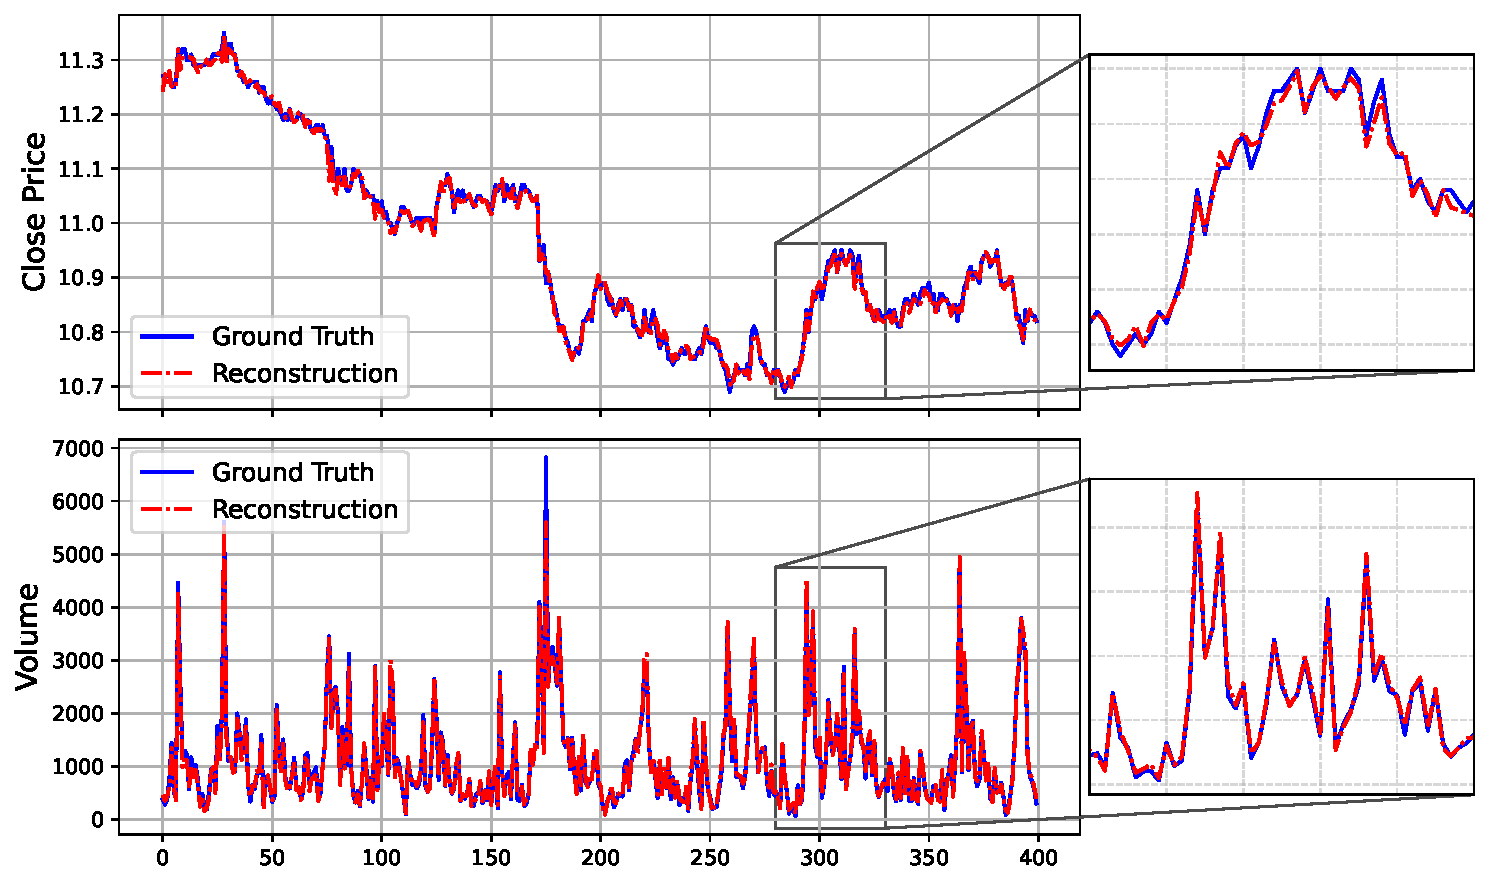
\includegraphics[width=\linewidth]{recon_imgs/pred_visualize_stock_XSHG_600977_5min.pdf}
        \caption{China Film Co.,Ltd. (SSE: 600977)}
    \end{subfigure}
    \hfill
    \begin{subfigure}[b]{0.49\textwidth}
        \centering
        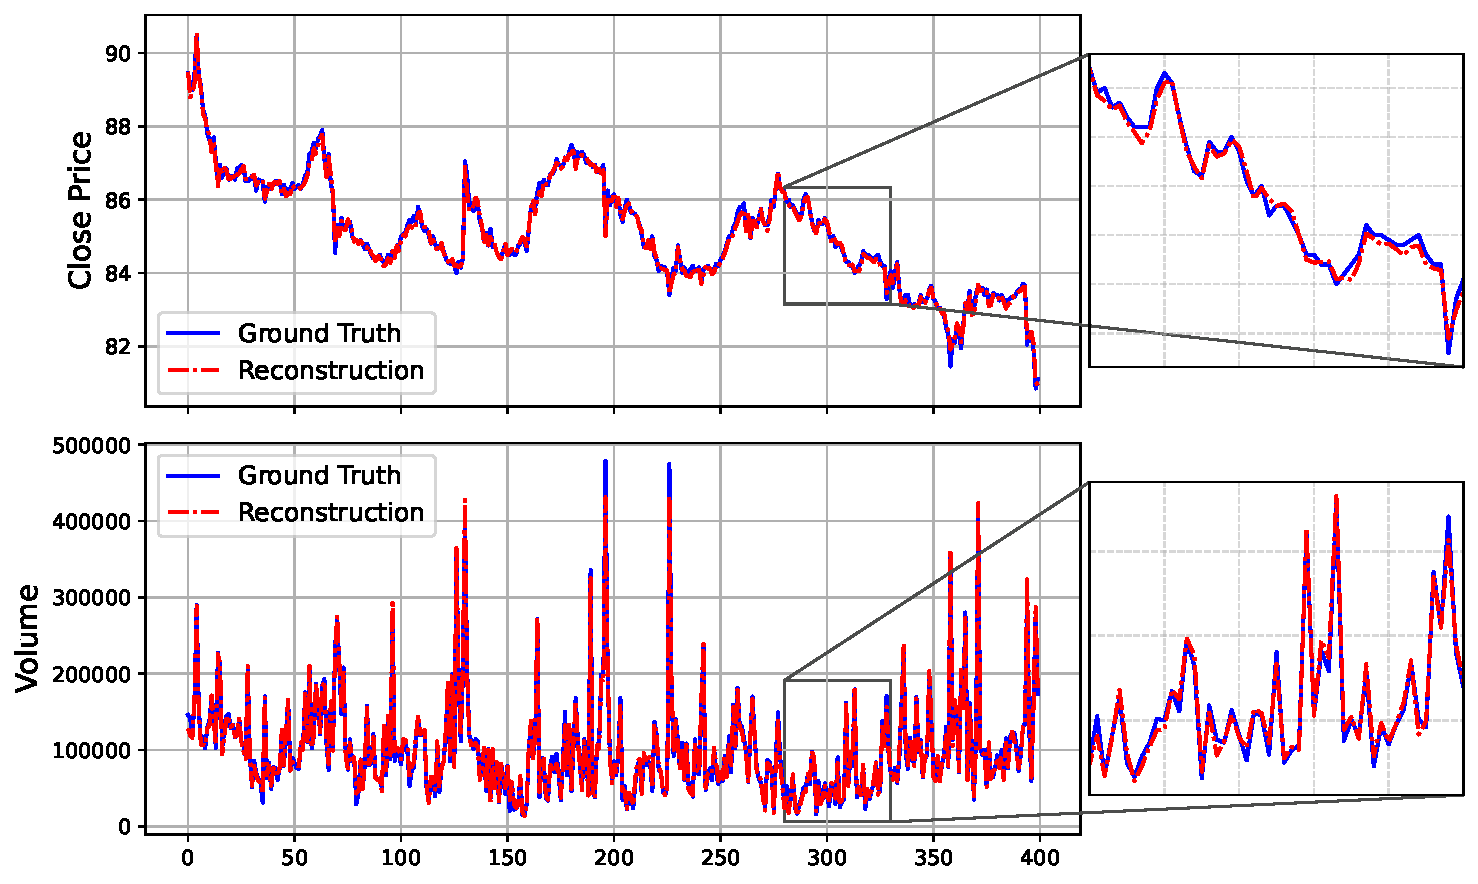
\includegraphics[width=\linewidth]{recon_imgs/pred_visualize_stock_XHKG_9992_5min.pdf}
        \caption{Pop Mart (HKEX: 09992)}
    \end{subfigure}

    \vspace{0.1cm}

    \begin{subfigure}[b]{0.49\textwidth}
        \centering
        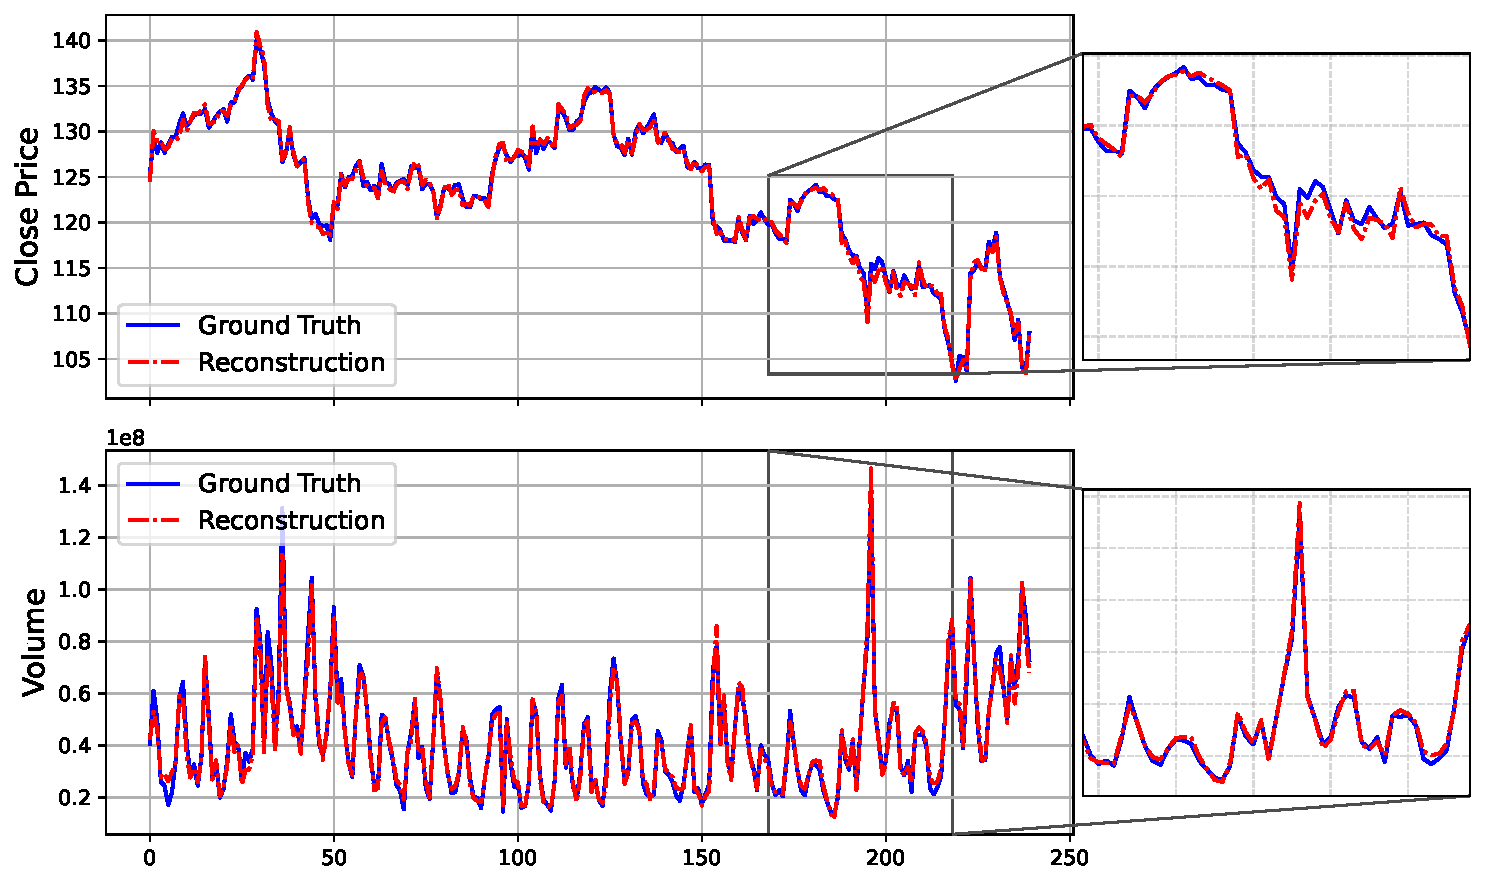
\includegraphics[width=\linewidth]{recon_imgs/pred_visualize_stock_XNAS_NVDA_60min.pdf}
        \caption{NVIDIA (NASDAQ: NVDA)}
    \end{subfigure}
    \hfill
    \begin{subfigure}[b]{0.49\textwidth}
        \centering
        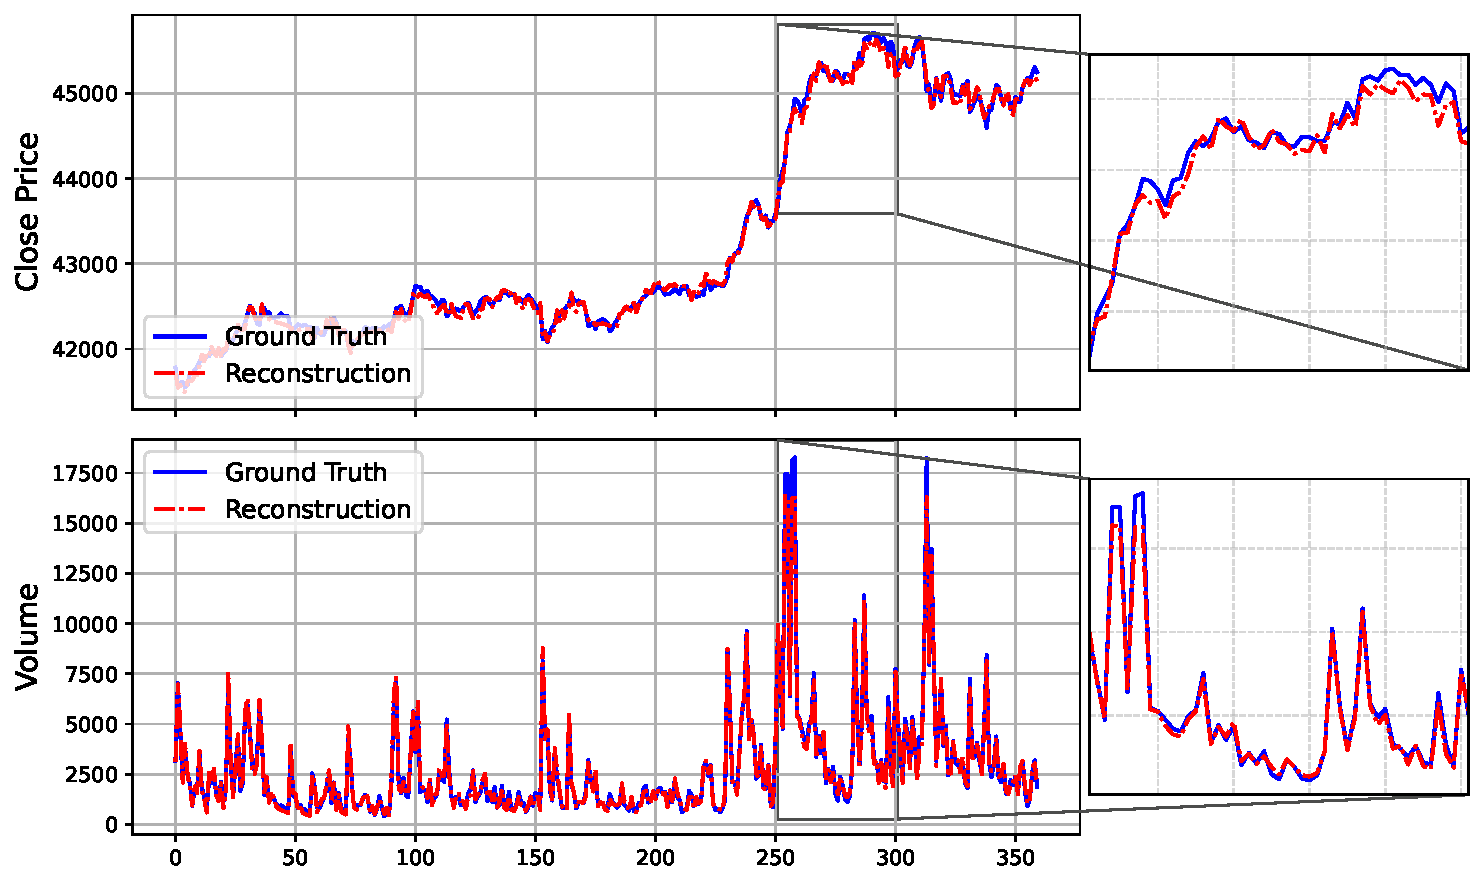
\includegraphics[width=\linewidth]{recon_imgs/pred_visualize_crypto_BTCUSDT_15min.pdf}
        \caption{BTC/USDT 무기한 (Binance: BTCUSDT)}
    \end{subfigure}

    \vspace{0.1cm}

    \begin{subfigure}[b]{0.49\textwidth}
        \centering
        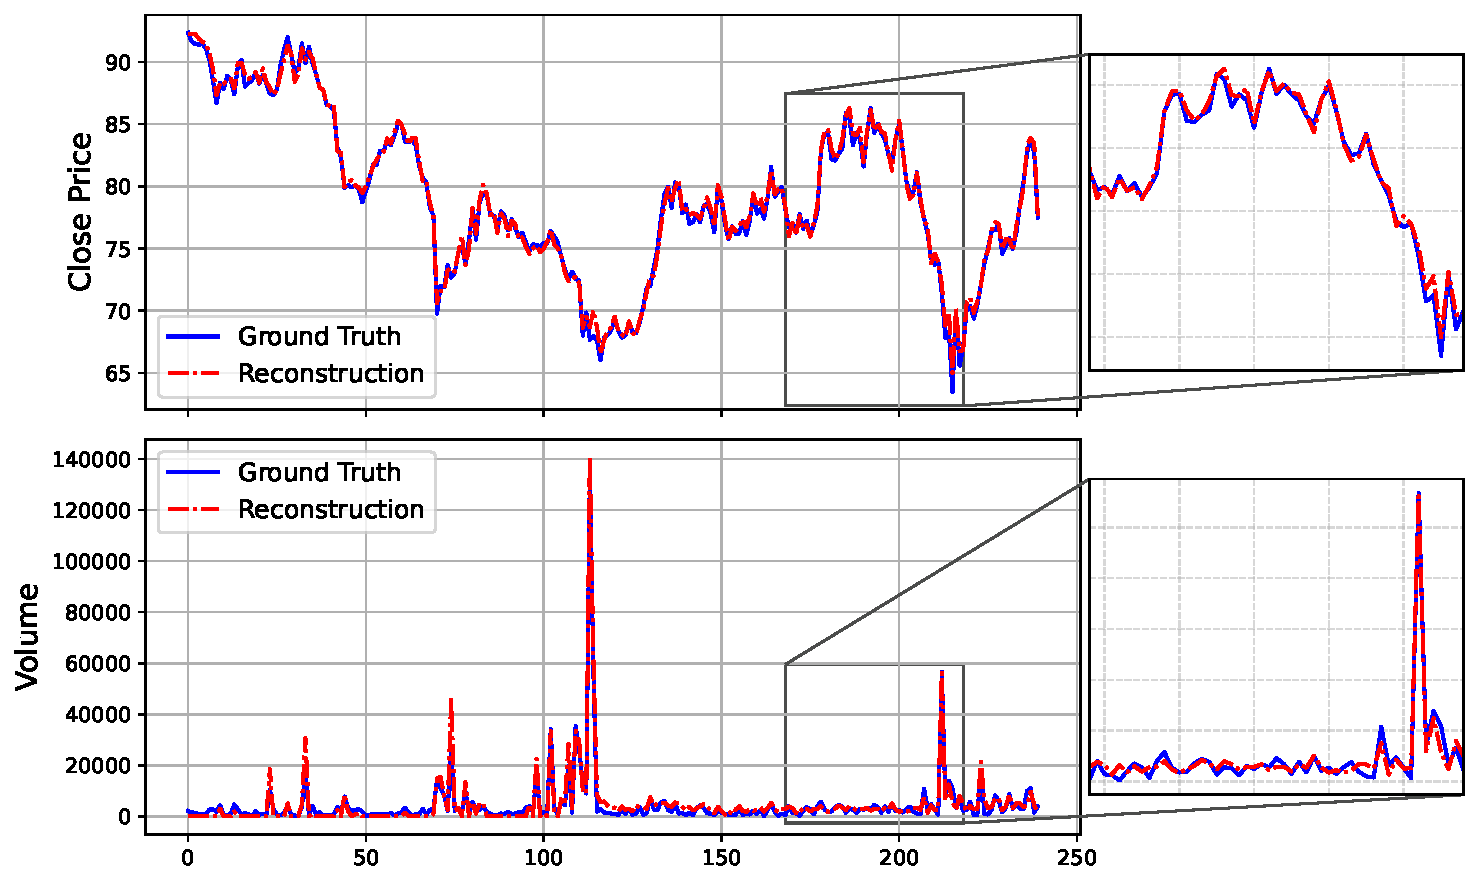
\includegraphics[width=\linewidth]{recon_imgs/pred_visualize_stock_XFRA_BMW_daily.pdf}
        \caption{BMW (FWB: BMW)}
    \end{subfigure}
    \hfill
    \begin{subfigure}[b]{0.49\textwidth}
        \centering
        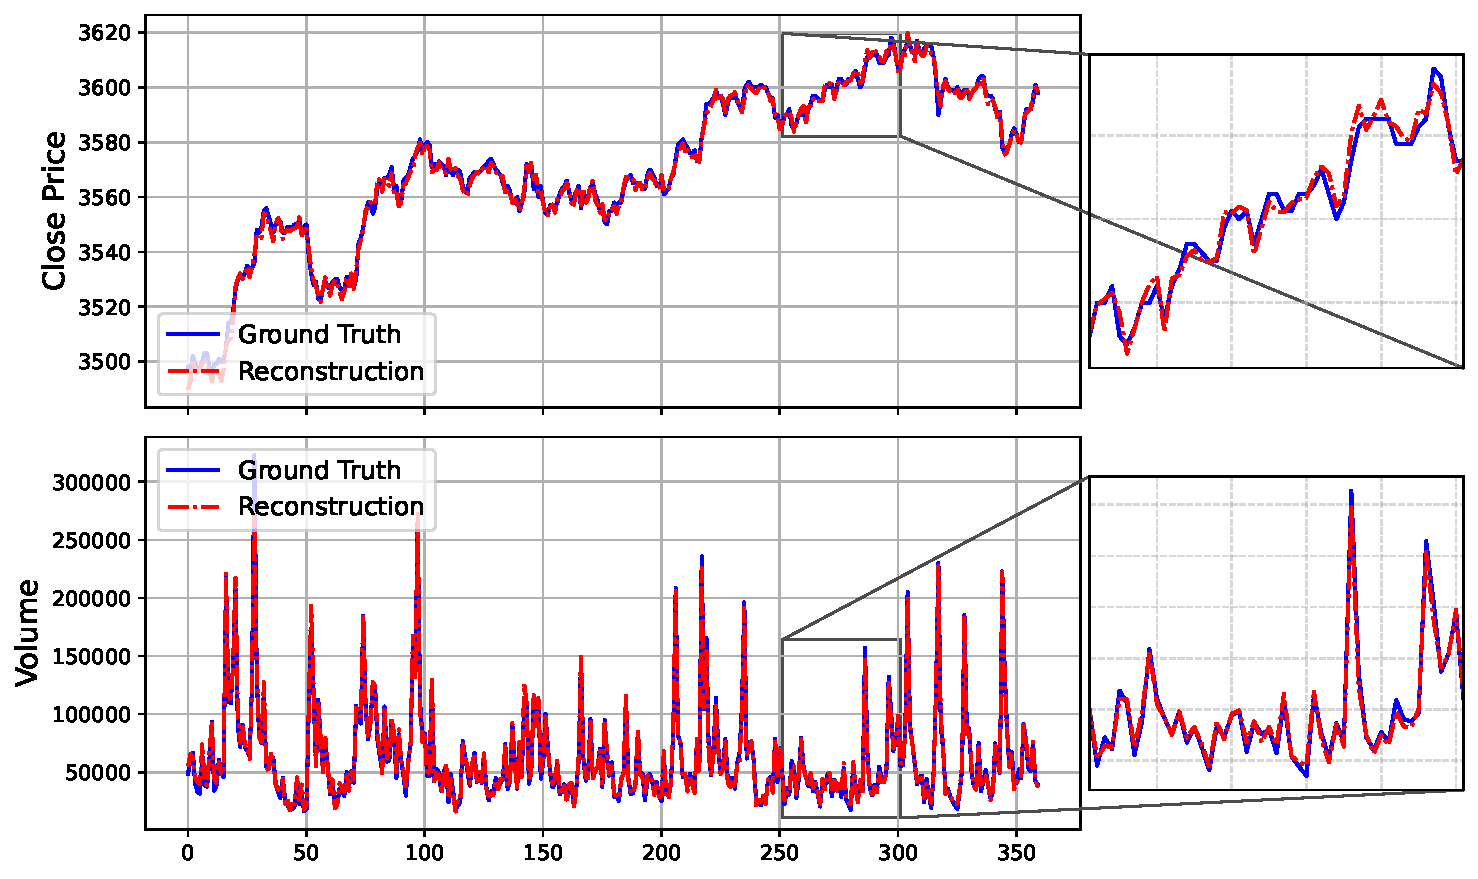
\includegraphics[width=\linewidth]{recon_imgs/pred_visualize_commodity_RB_5min.pdf}
        \caption{철근 선물 (SHFE: RB)}
    \end{subfigure}

    \vspace{0.1cm}

    \caption{K-line Tokenizer가 생성한 `Close Price'와 `Volume'의 재구성 결과 시각화. \textcolor{blue}{Blue} 선은 정답값을 나타내며, \textcolor{red}{red} 선은 우리 모델이 생성한 재구성 결과를 나타낸다.}
    \label{fig:recon_case}
\end{figure*}




\begin{figure*}[htbp]
    \centering

    \begin{subfigure}{\textwidth}
        \centering
        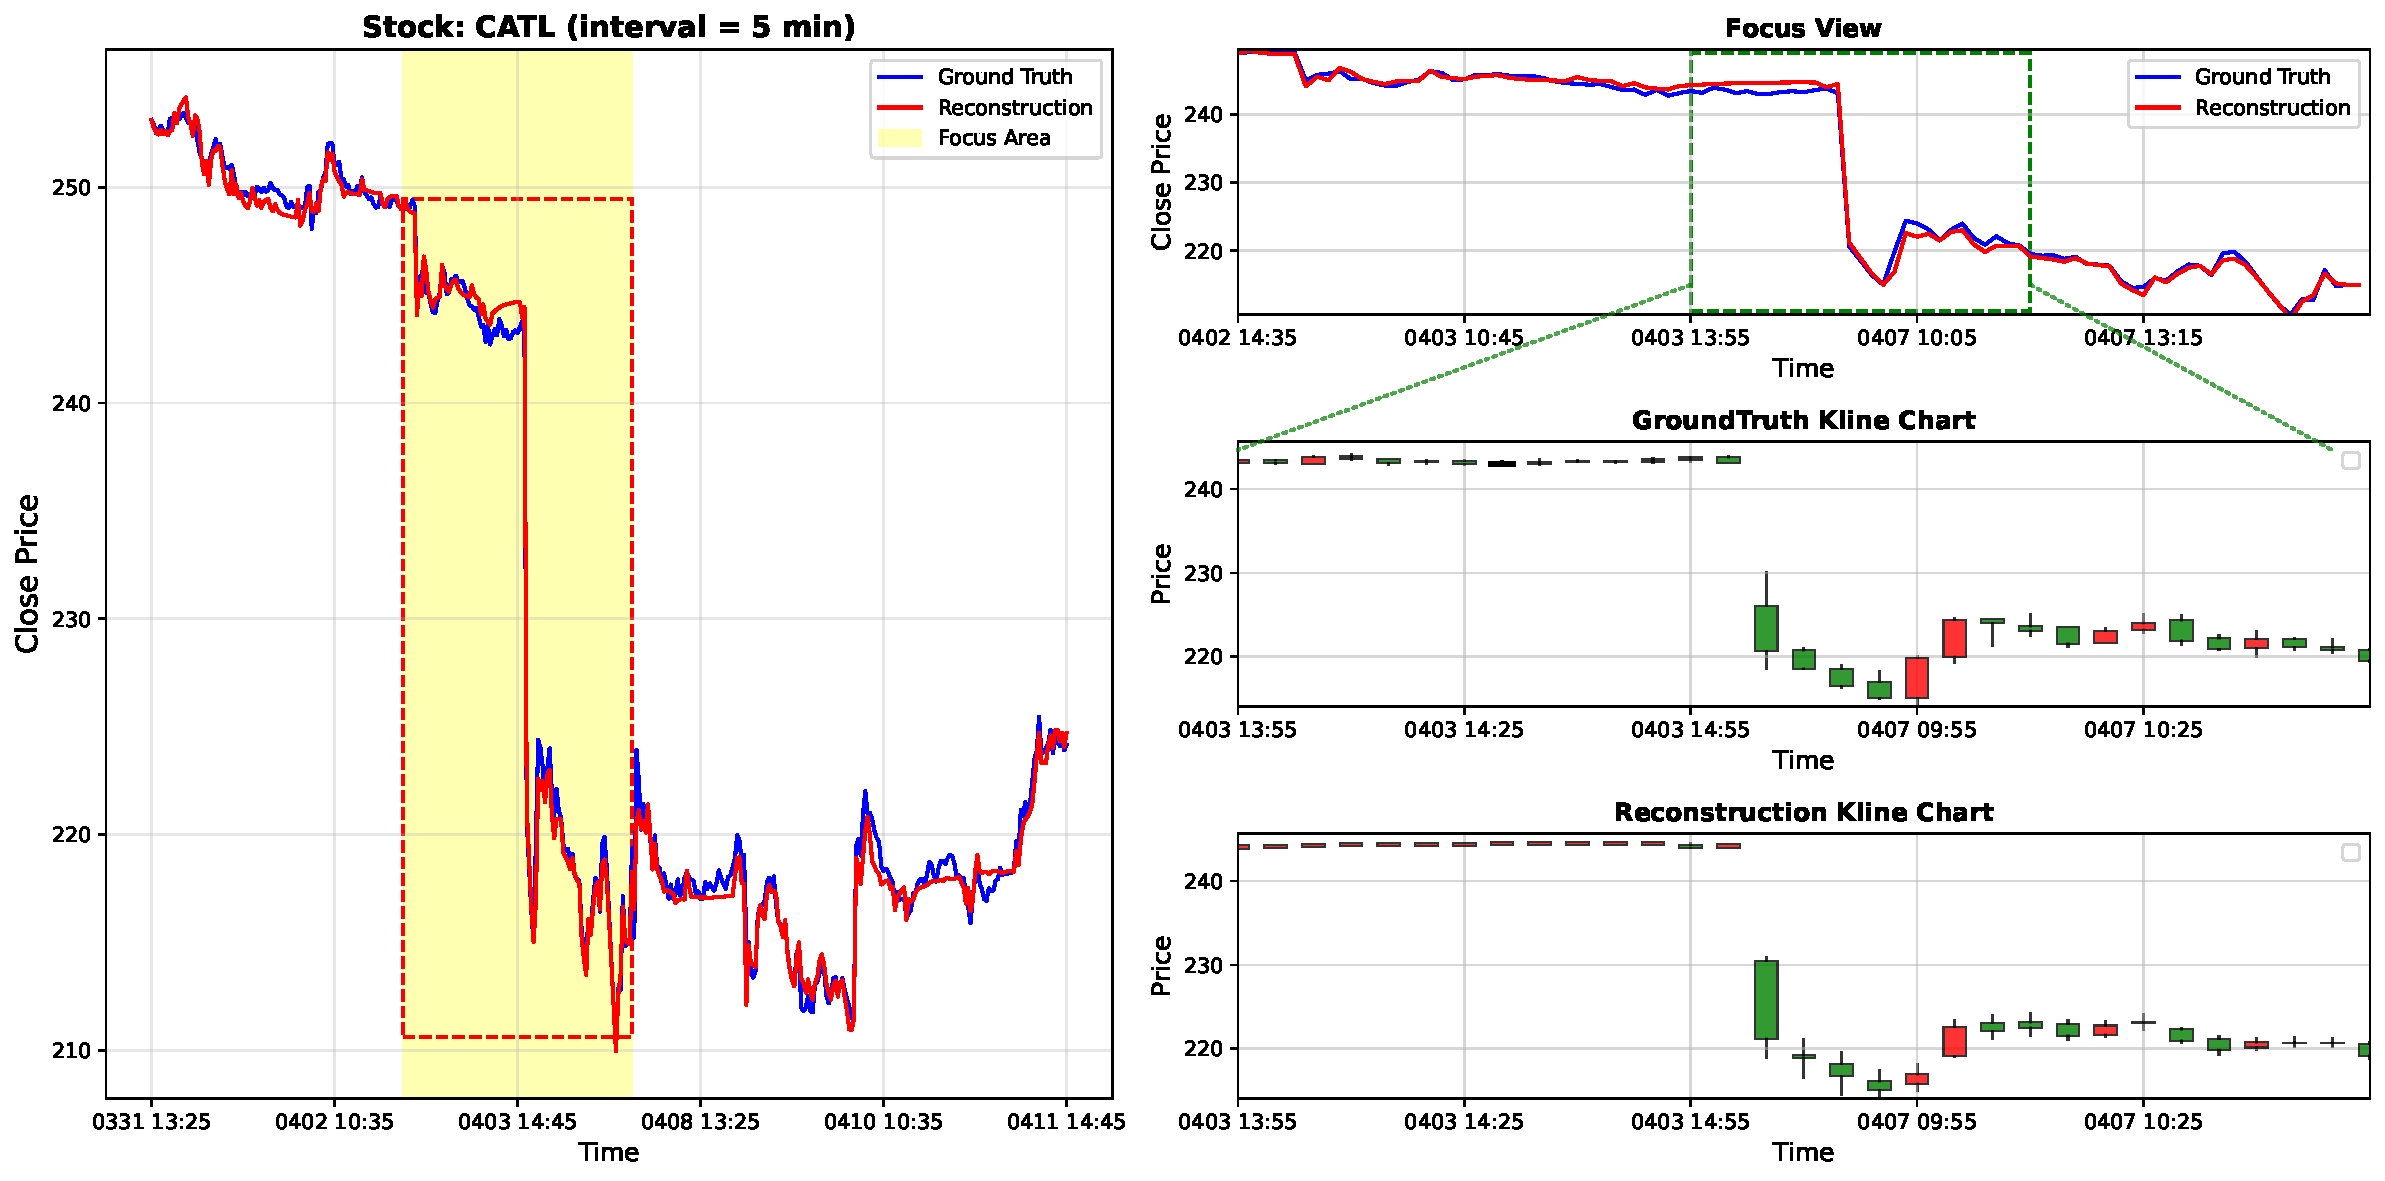
\includegraphics[width=1.0\textwidth]{recon_imgs/cn_300750_5min_shocks_price_release.pdf}
        \caption{주식 K-line 재구성, 가격 부분 }
    \end{subfigure}

    \begin{subfigure}{\textwidth}
        \centering
        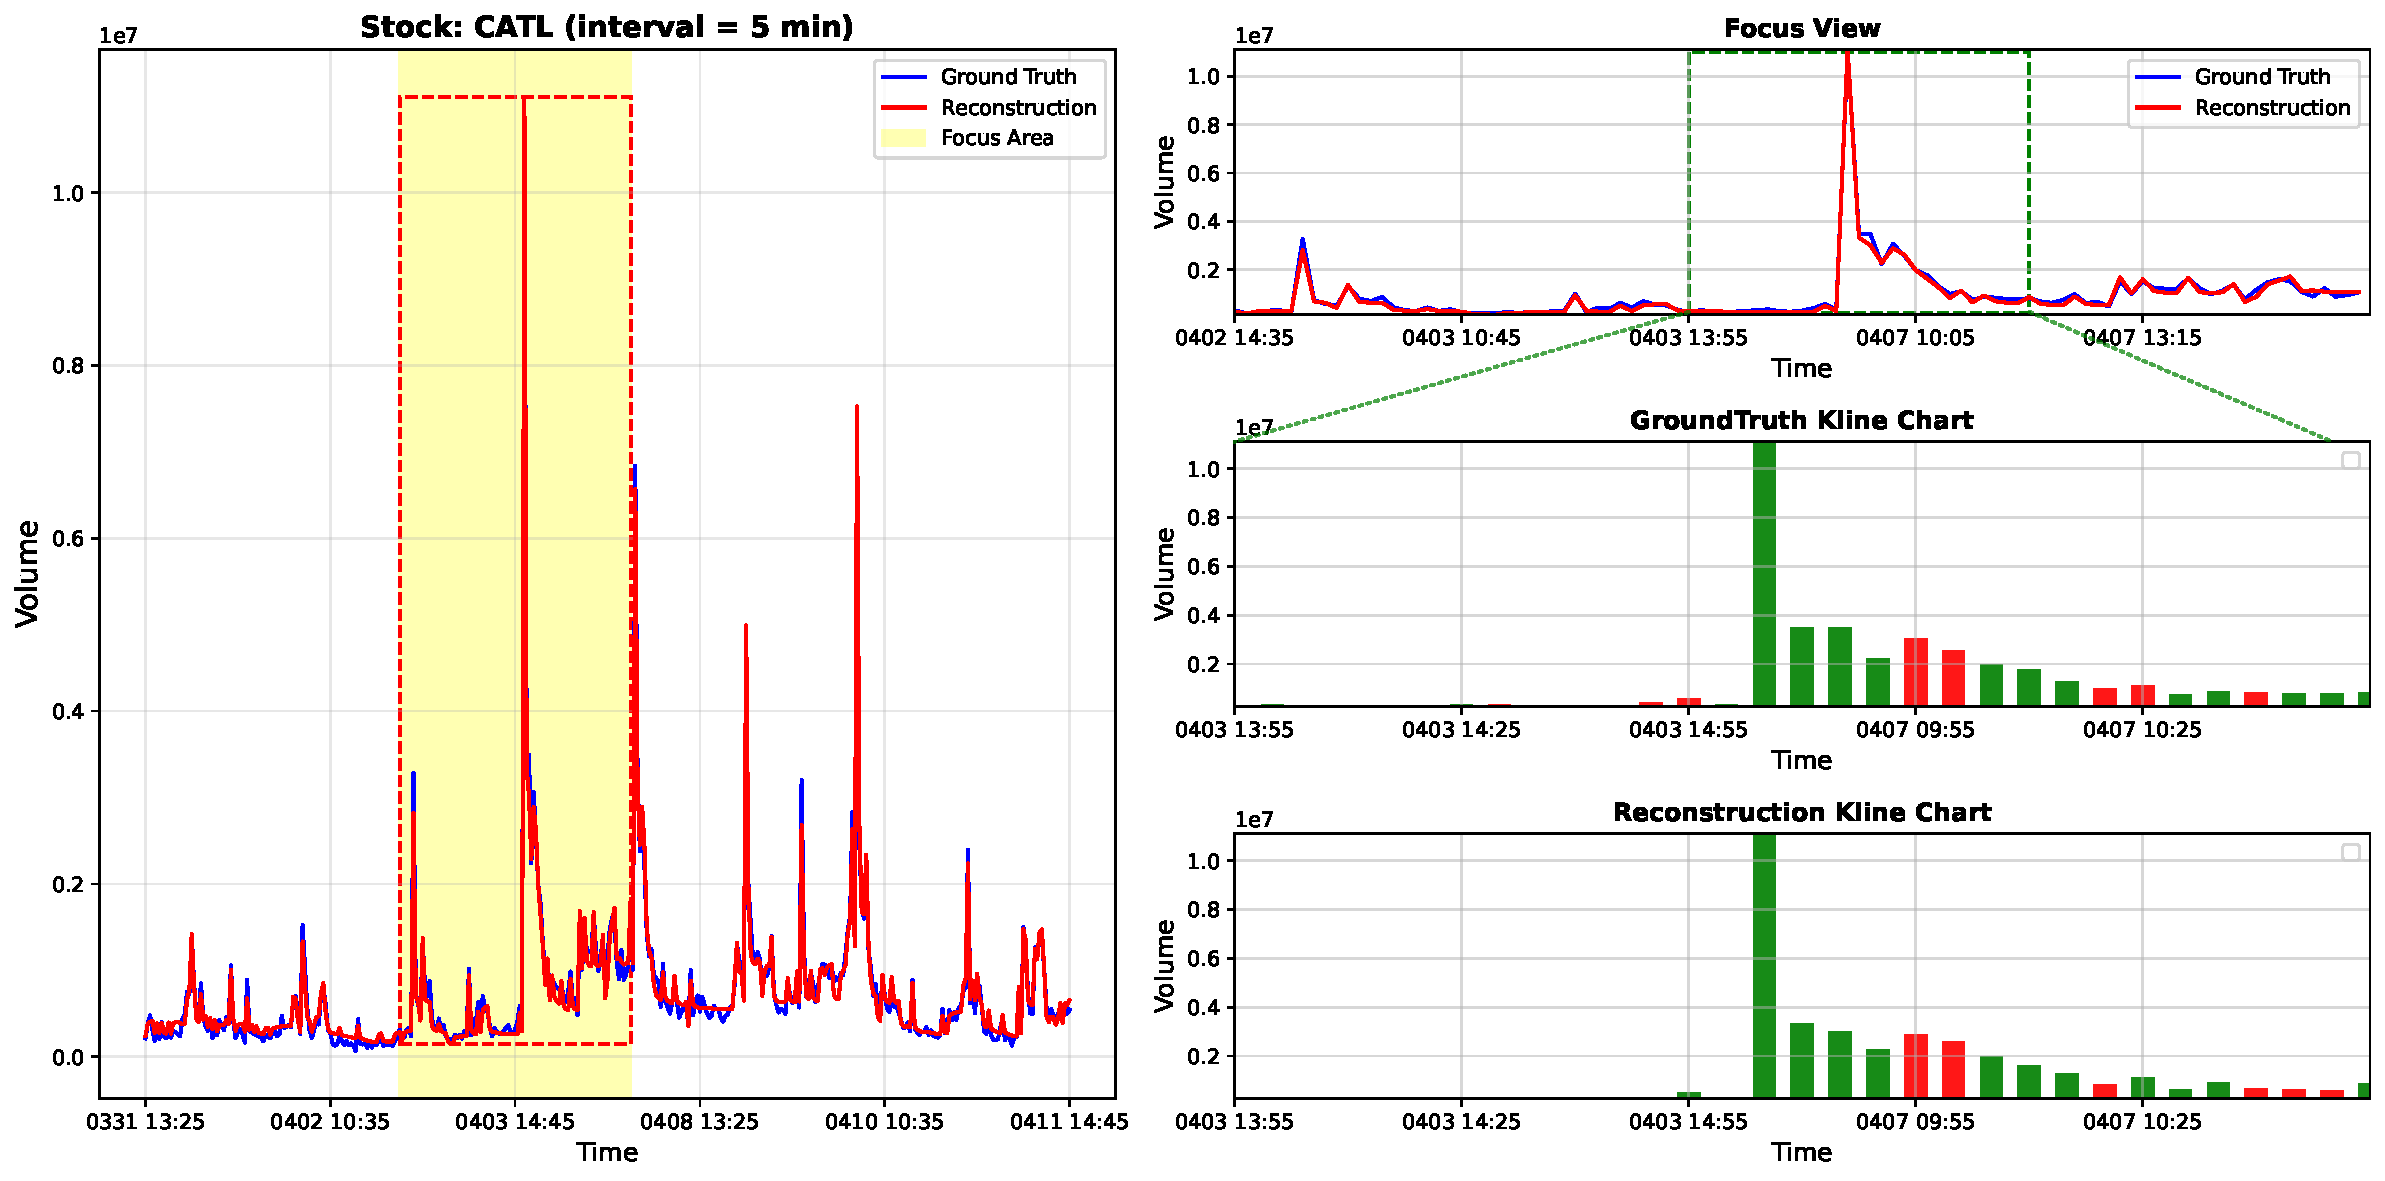
\includegraphics[width=1.0\textwidth]{recon_imgs/cn_300750_5min_shocks_volume_release.pdf}
        \caption{주식 K-line 재구성, 거래량 부분}
    \end{subfigure}

    \vspace{0.1cm}


    \caption{
    Trump의 무역전쟁~\cite{mckibbin2025global}이라는 경제적 맥락에서 2025년 4월 7일 CATL (Contemporary Amperex Technology Co., Limited)의 5분 K-line 데이터 재구성 성능을 보여 주는 예시. 시각화에서 캔들스틱은 ``상승은 빨간색, 하락은 초록색'' 관례를 따르며(상승/하락은 시가 대비 종가로 결정됨), 거래량 막대도 이에 맞추어 색칠된다.
    }
    \label{fig:kline_reconstruction_tradewar}
\end{figure*}







\twocolumn

% \begin{figure*}[ht]
%     \centering

%     \begin{subfigure}[b]{0.32\textwidth}
%         \centering
%         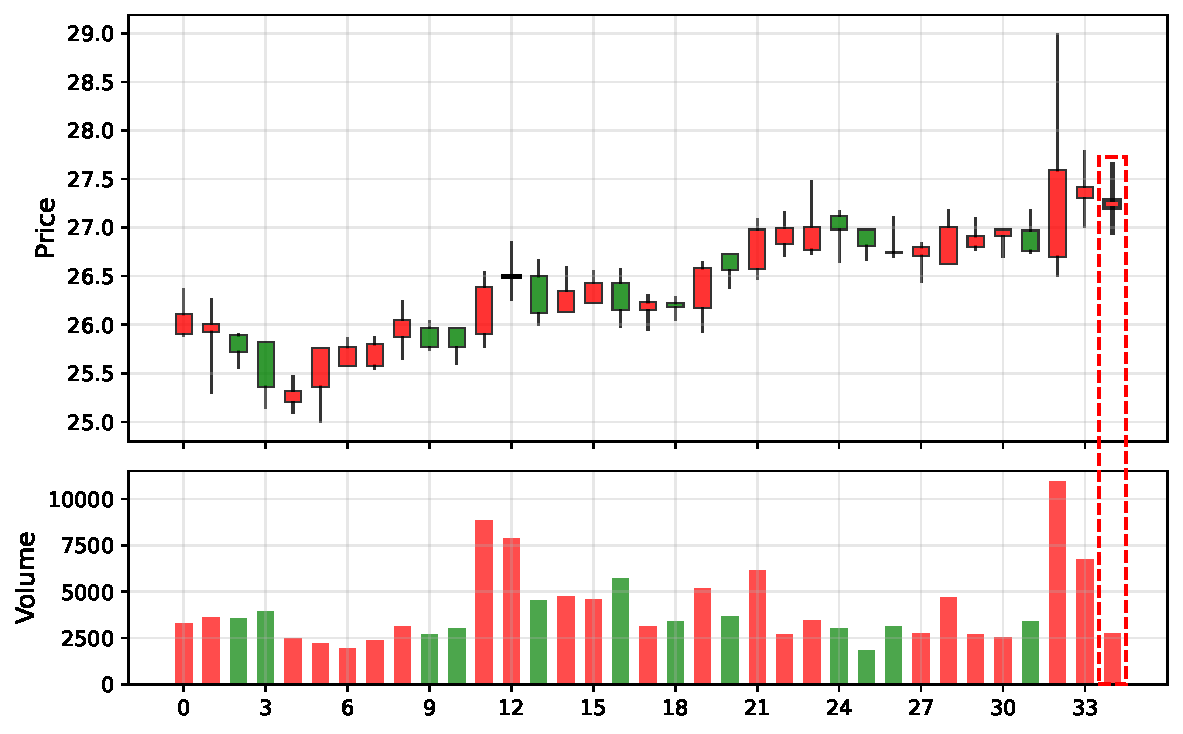
\includegraphics[width=\linewidth]{tokens/high_used_token_1.pdf}
%         \caption{빈도가 높은 토큰 예시 1}
%     \end{subfigure}
%     \hfill
%     \begin{subfigure}[b]{0.32\textwidth}
%         \centering
%         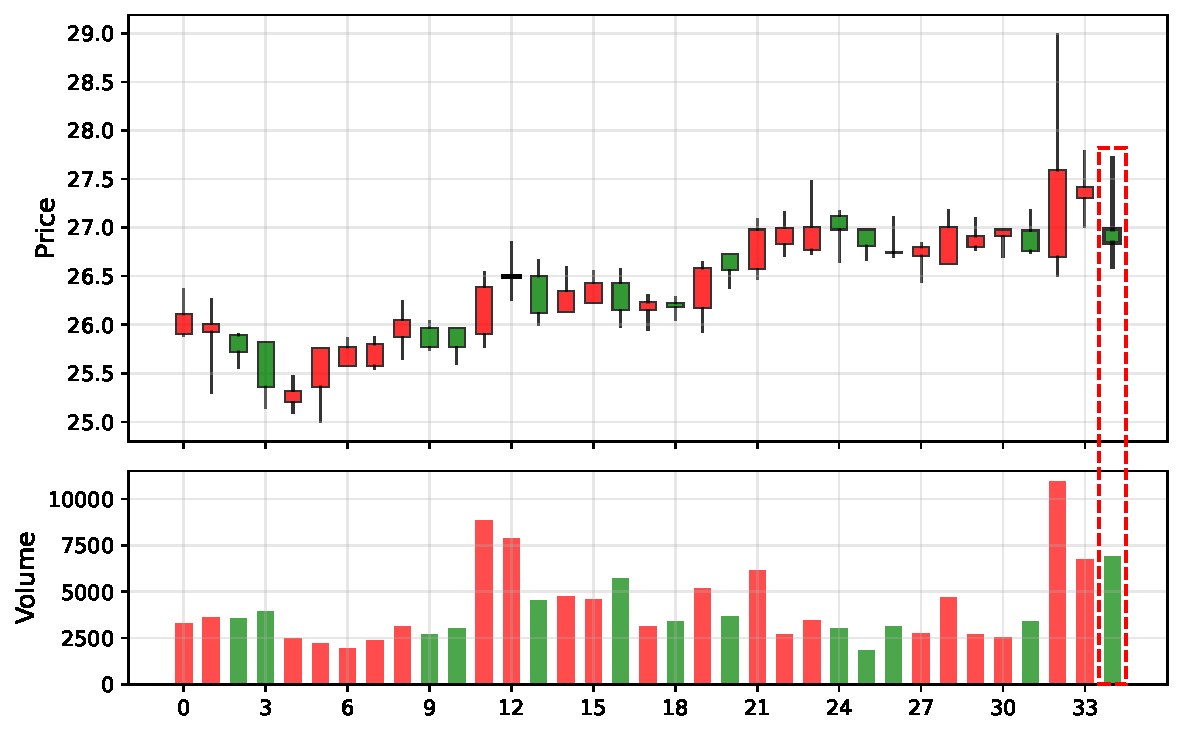
\includegraphics[width=\linewidth]{tokens/high_used_token_2.pdf}
%         \caption{빈도가 높은 토큰 예시 2}
%     \end{subfigure}
%     \hfill
%     \begin{subfigure}[b]{0.32\textwidth}
%         \centering
%         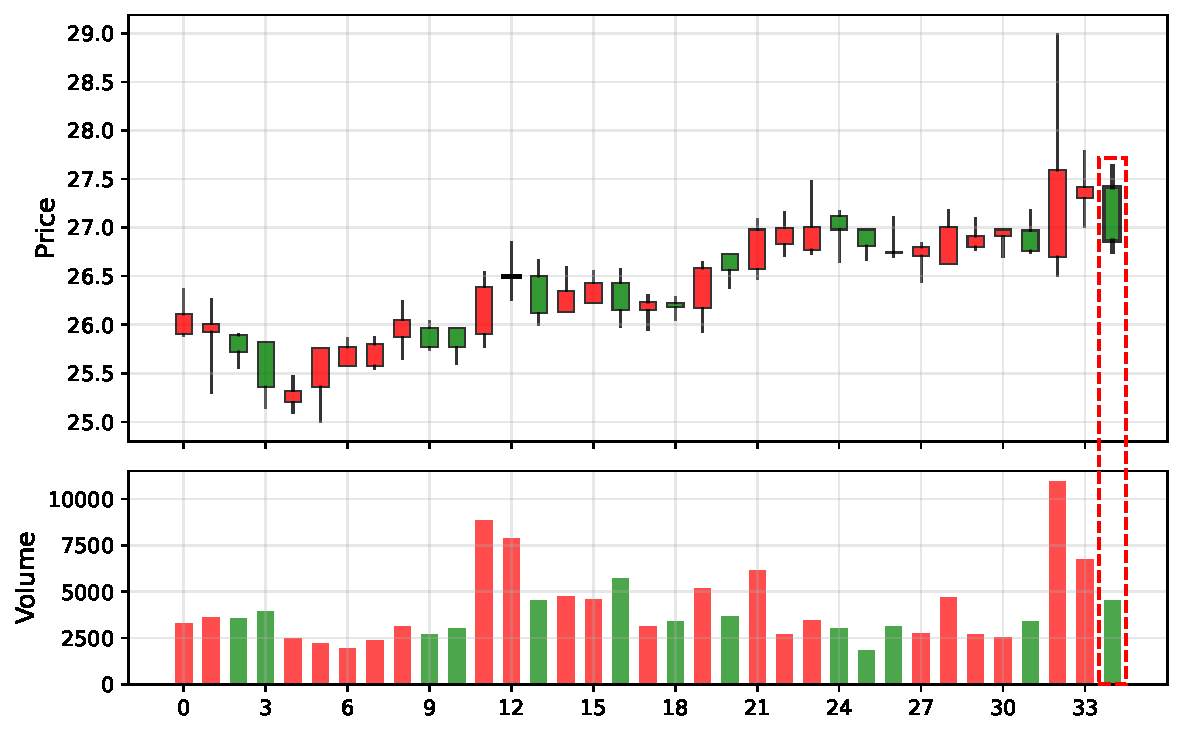
\includegraphics[width=\linewidth]{tokens/high_used_token_3.pdf}
%         \caption{빈도가 높은 토큰 예시 3}
%     \end{subfigure}

%     \vspace{0.1cm}

%     \begin{subfigure}[b]{0.32\textwidth}
%         \centering
%         \includegraphics[width=\linewidth]{tokens/low_usage_token_1.pdf}
%         \caption{빈도가 낮은 토큰 예시 1}
%     \end{subfigure}
%     \hfill
%     \begin{subfigure}[b]{0.32\textwidth}
%         \centering
%         \includegraphics[width=\linewidth]{tokens/low_usage_token_2.pdf}
%         \caption{빈도가 낮은 토큰 예시 2}
%     \end{subfigure}
%     \hfill
%     \begin{subfigure}[b]{0.32\textwidth}
%         \centering
%         \includegraphics[width=\linewidth]{tokens/low_usage_token_3.pdf}
%         \caption{빈도가 낮은 토큰 예시 3}
%     \end{subfigure}

%     \vspace{0.1cm}

%     \begin{subfigure}[b]{0.32\textwidth}
%         \centering
%         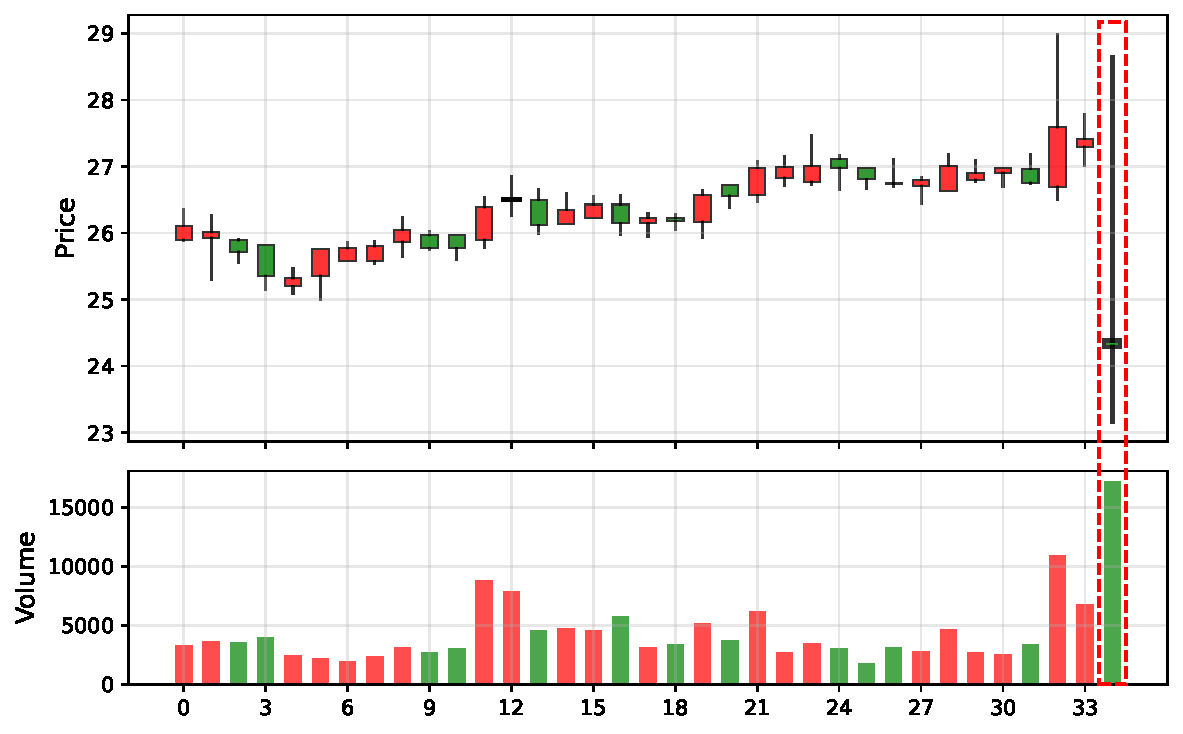
\includegraphics[width=\linewidth]{tokens/unused_token_1.pdf}
%         \caption{사용되지 않은 토큰 예시 1}
%     \end{subfigure}
%     \hfill
%     \begin{subfigure}[b]{0.32\textwidth}
%         \centering
%         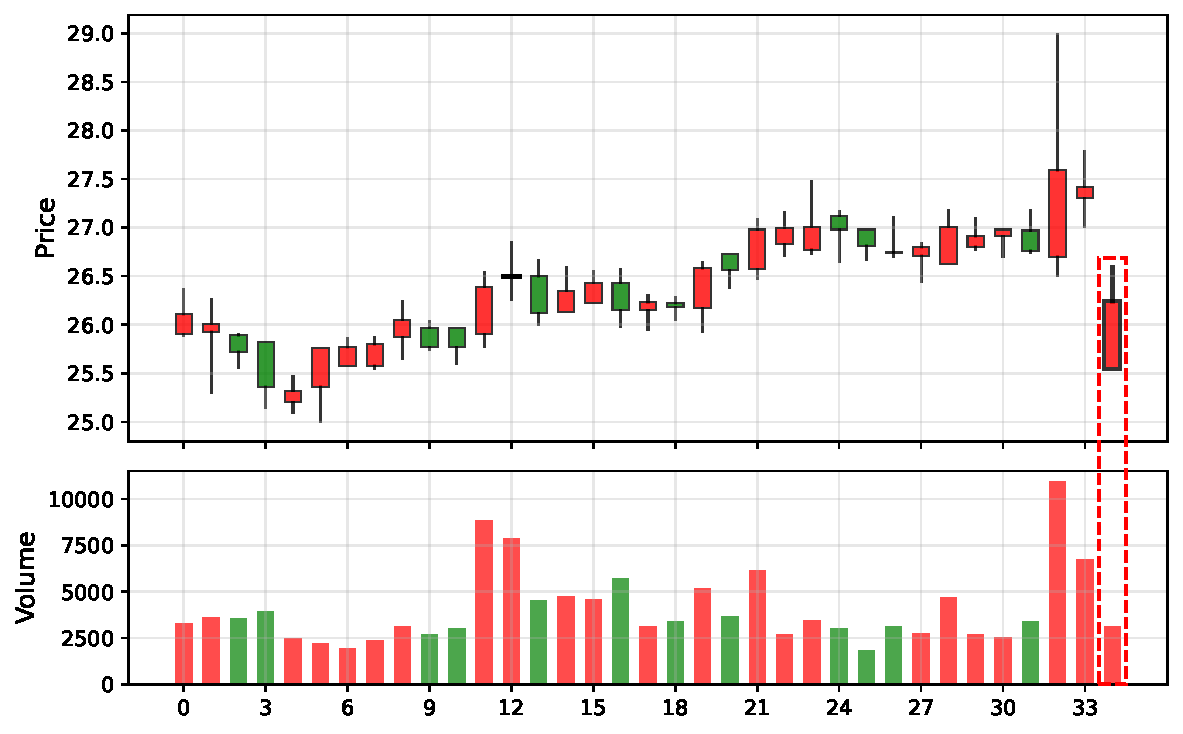
\includegraphics[width=\linewidth]{tokens/unused_token_2.pdf}
%         \caption{사용되지 않은 토큰 예시 2}
%     \end{subfigure}
%     \hfill
%     \begin{subfigure}[b]{0.32\textwidth}
%         \centering
%         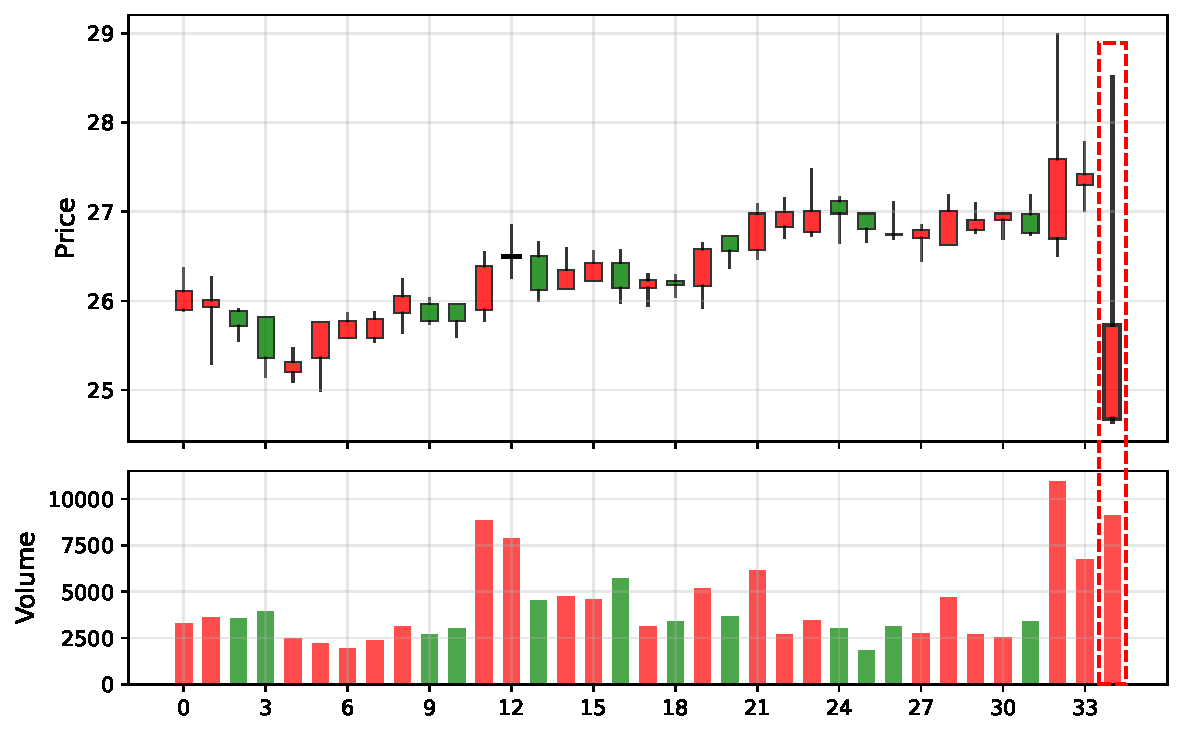
\includegraphics[width=\linewidth]{tokens/unused_token_3.pdf}
%         \caption{사용되지 않은 토큰 예시 3}
%     \end{subfigure}
%     \vspace{0.1cm}


%     \begin{subfigure}[b]{0.32\textwidth}
%         \centering
%         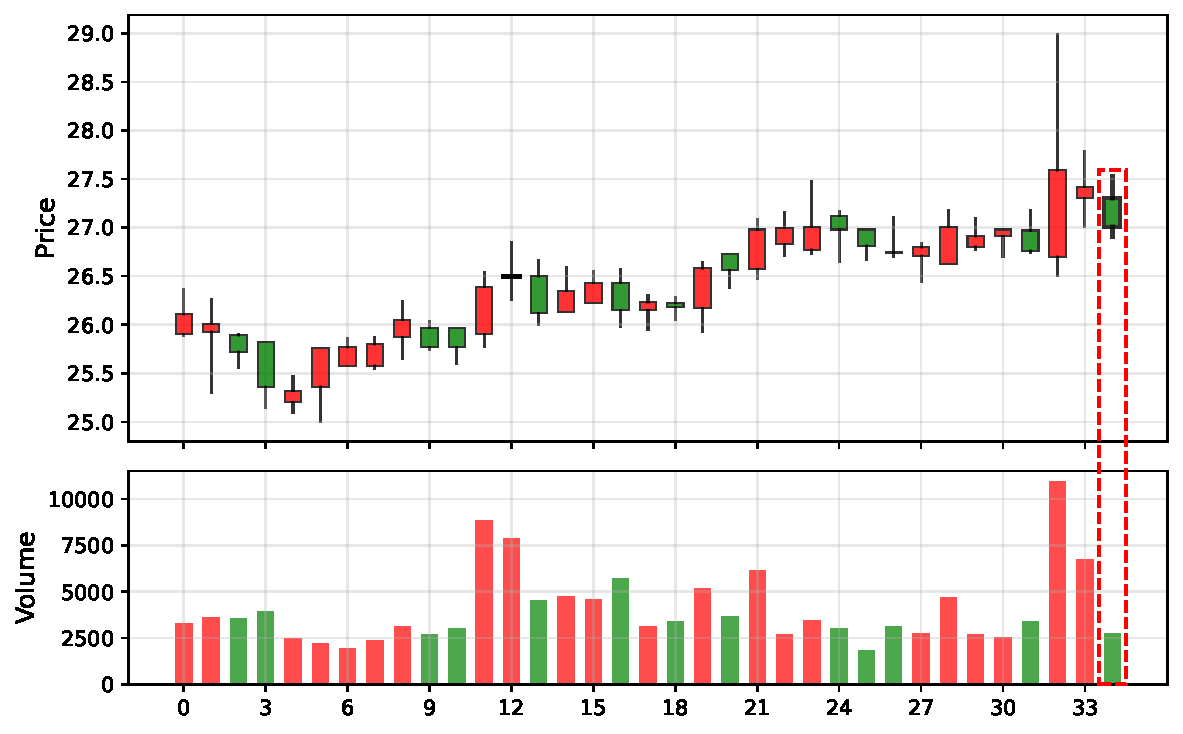
\includegraphics[width=\linewidth]{tokens/original_kline.pdf}
%         \caption{원본 토큰 시퀀스 샘플}
%     \end{subfigure}


%     \caption{토큰 예시}
%     \label{fig:token_show_case}
% \end{figure*}



\begin{figure*}[ht]
    \centering

    % 그룹 1: 고빈도 토큰
    \begin{subfigure}[b]{\textwidth}
        \centering
        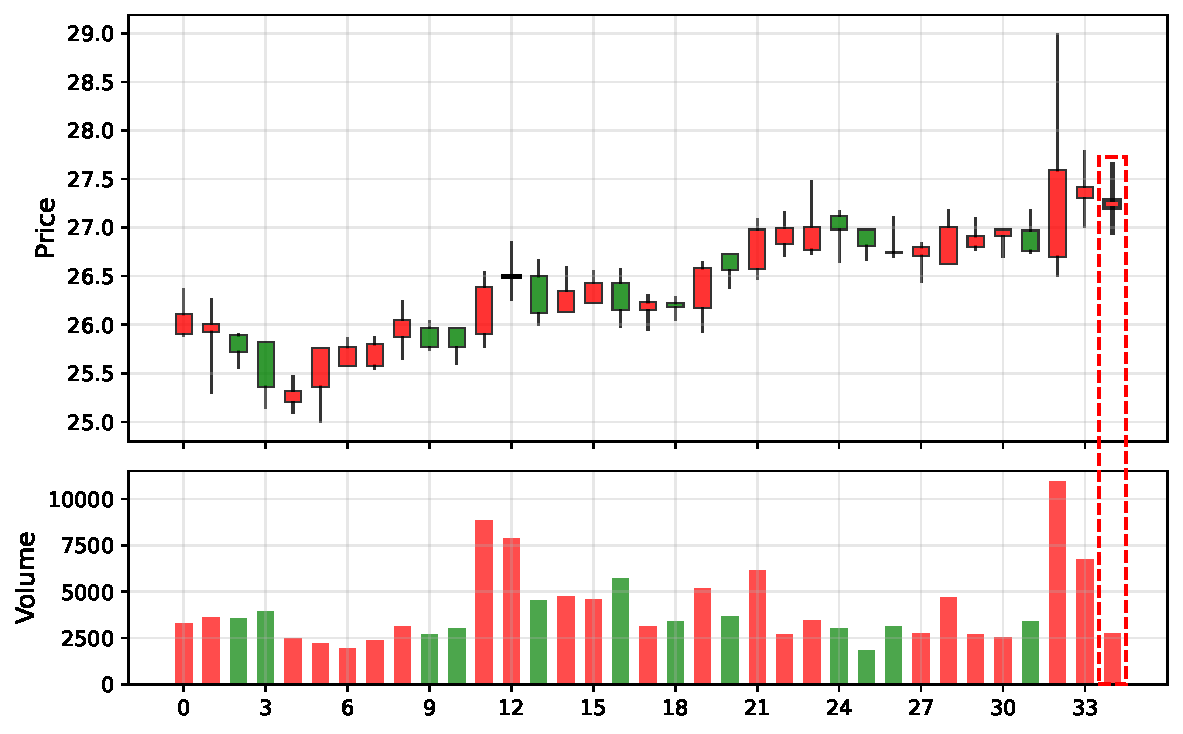
\includegraphics[width=0.32\textwidth]{tokens/high_used_token_1.pdf}
        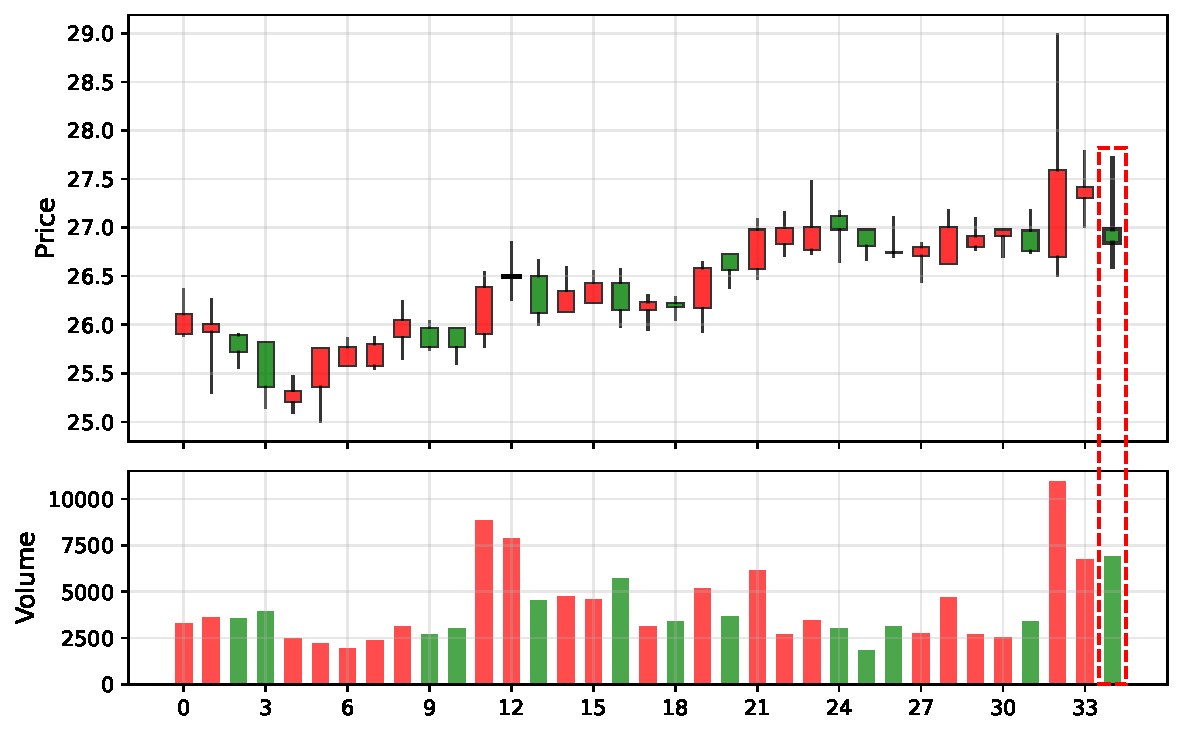
\includegraphics[width=0.32\textwidth]{tokens/high_used_token_2.pdf}
        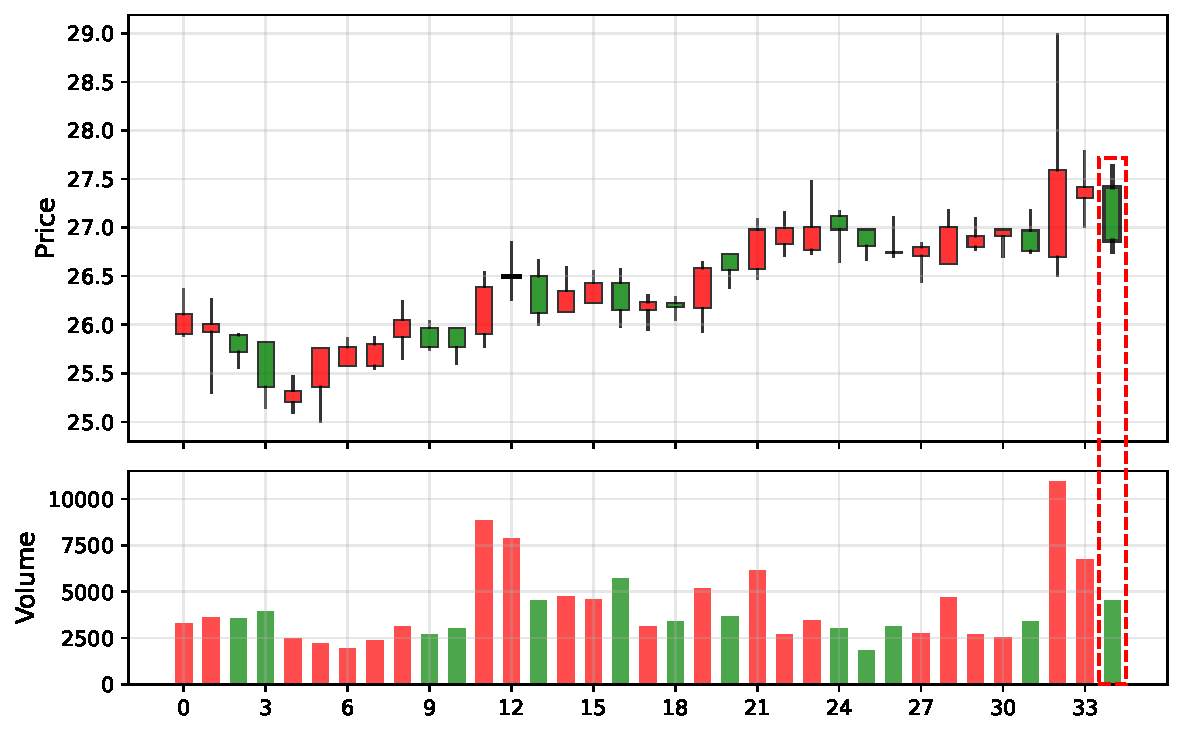
\includegraphics[width=0.32\textwidth]{tokens/high_used_token_3.pdf}
        \caption{고빈도 토큰의 예시.}
    \end{subfigure}
    \vspace{0.1cm}

    % 그룹 2: 저빈도 토큰
    \begin{subfigure}[b]{\textwidth}
        \centering
        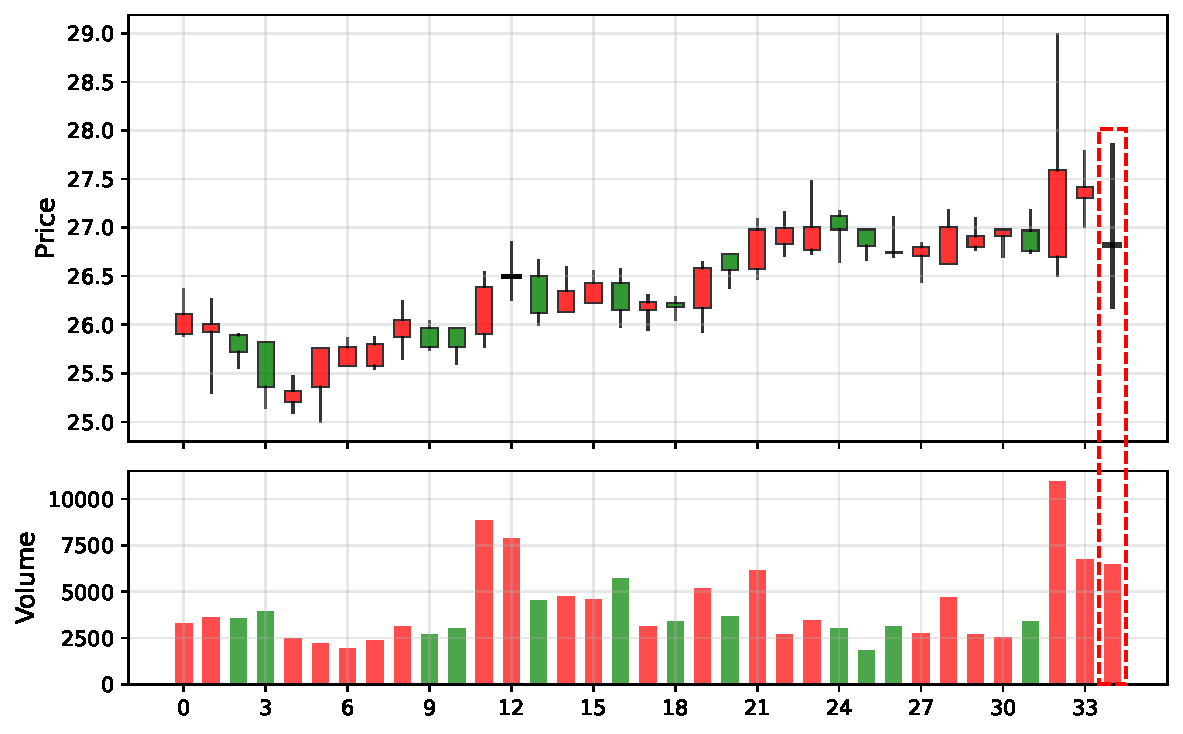
\includegraphics[width=0.32\textwidth]{tokens/low_used_token_1.pdf}
        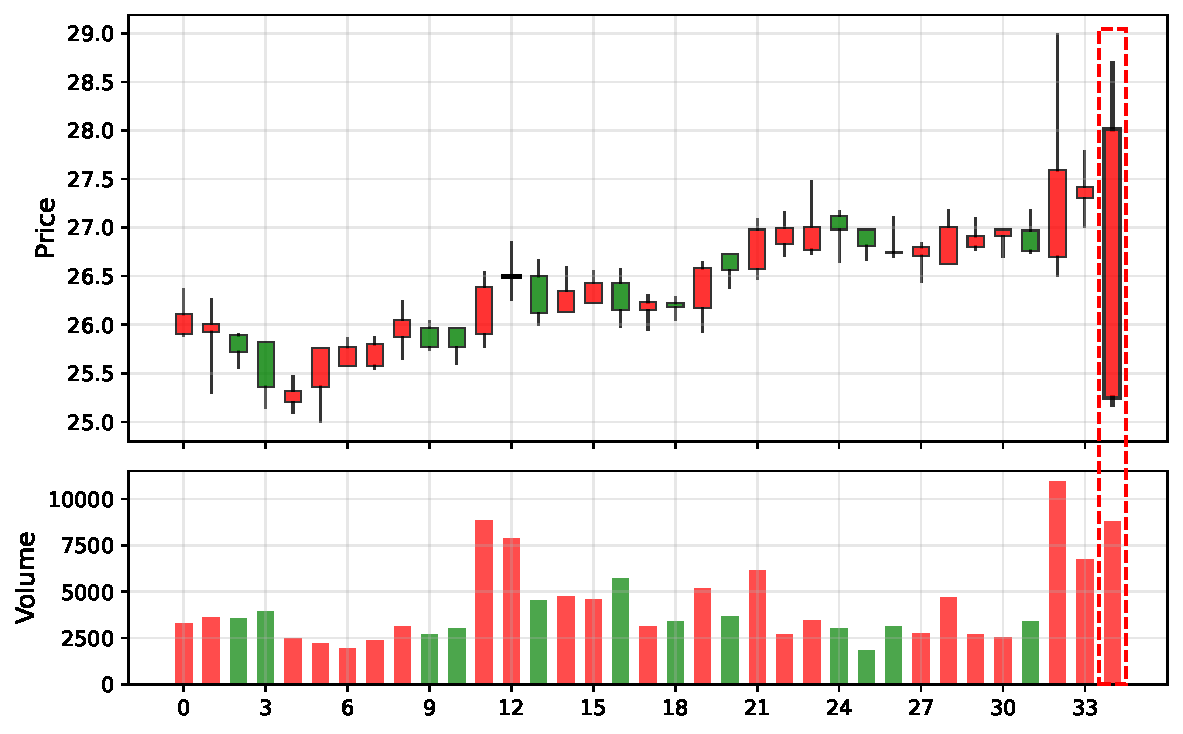
\includegraphics[width=0.32\textwidth]{tokens/low_used_token_2.pdf}
        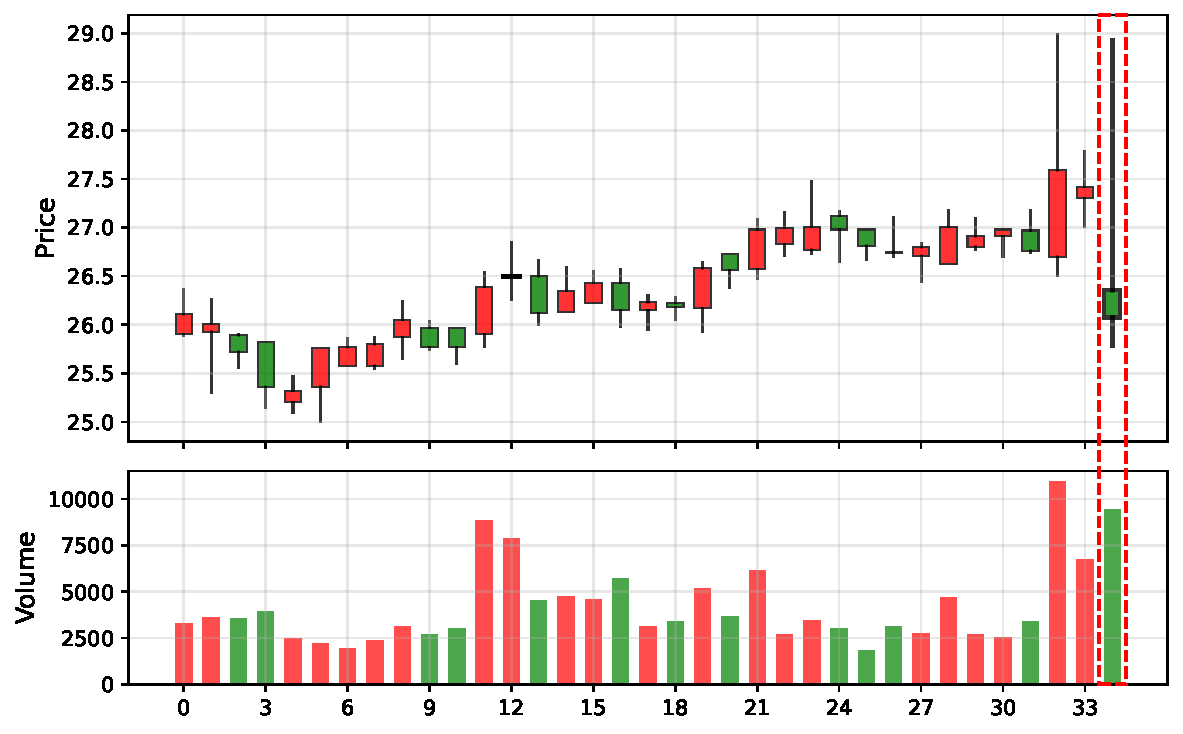
\includegraphics[width=0.32\textwidth]{tokens/low_used_token_3.pdf}
        \caption{저빈도 토큰의 예시.}
    \end{subfigure}
    \vspace{0.1cm}

    % 그룹 3: 사용되지 않은 토큰
    \begin{subfigure}[b]{\textwidth}
        \centering
        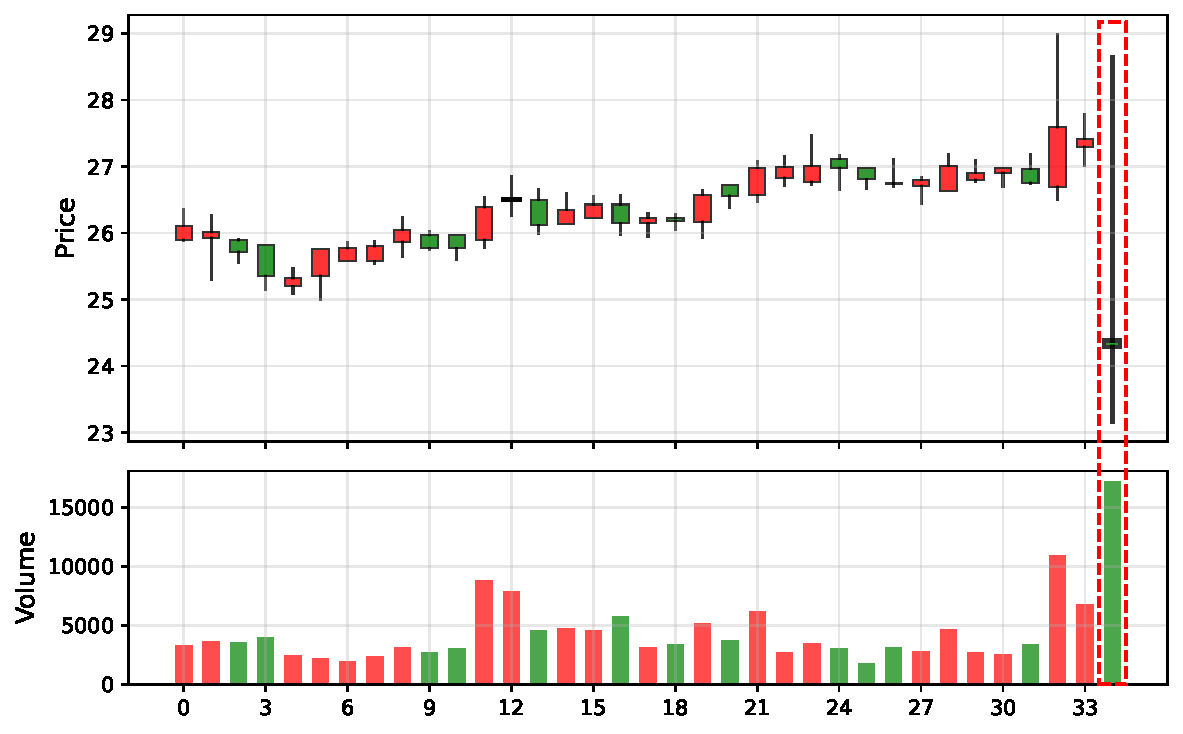
\includegraphics[width=0.32\textwidth]{tokens/unused_token_1.pdf}
        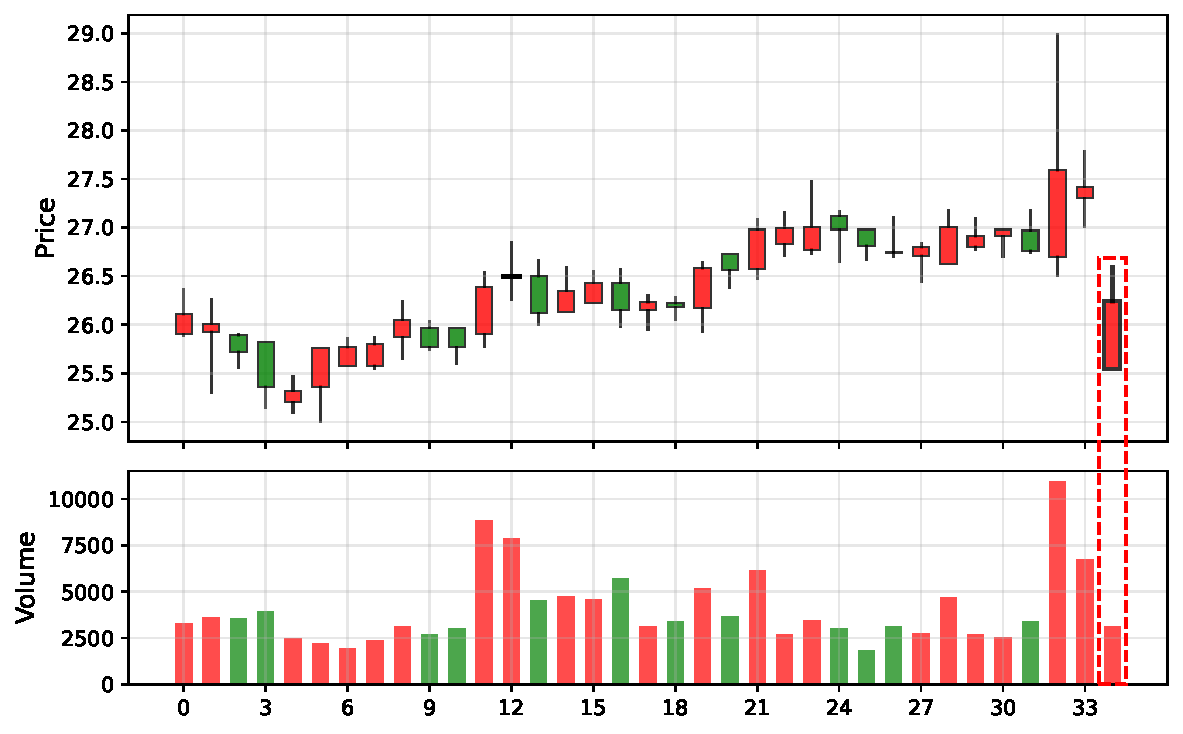
\includegraphics[width=0.32\textwidth]{tokens/unused_token_2.pdf}
        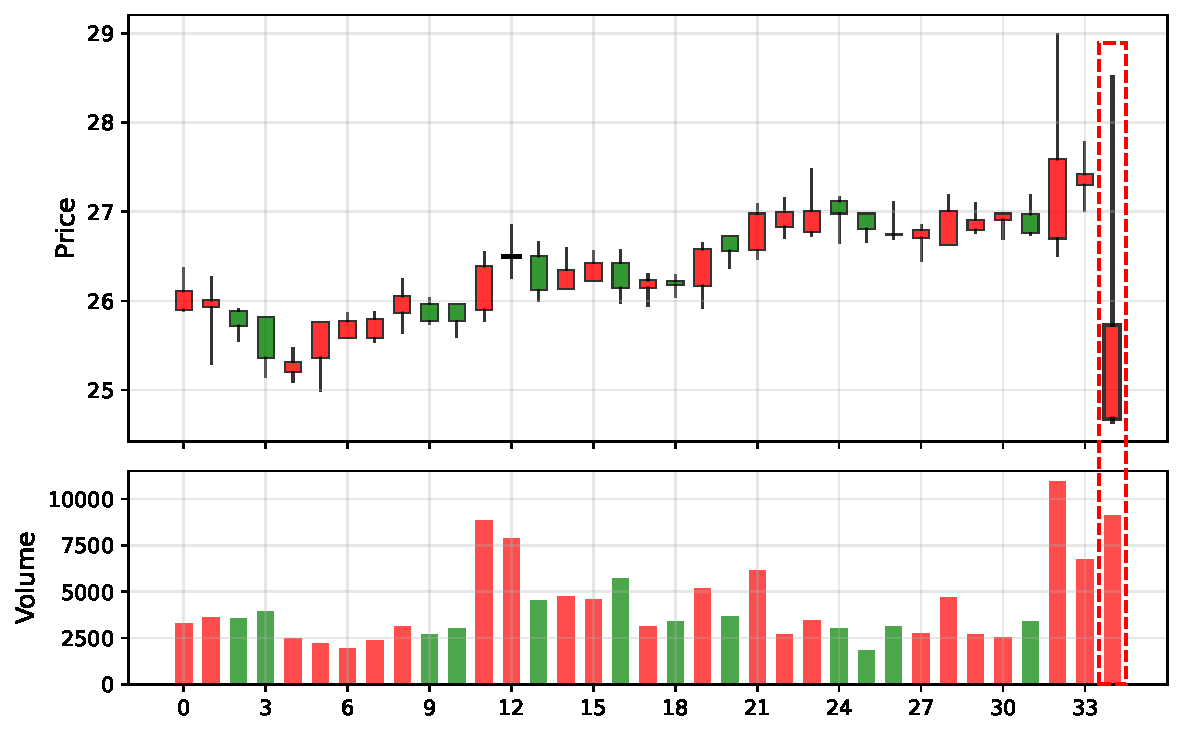
\includegraphics[width=0.32\textwidth]{tokens/unused_token_3.pdf}
        \caption{어휘집에서 사용되지 않은 토큰의 예시.}
    \end{subfigure}
    \vspace{0.1cm}

    % 그룹 4: 원본 토큰 시퀀스
    \begin{subfigure}[b]{\textwidth}
        \centering
        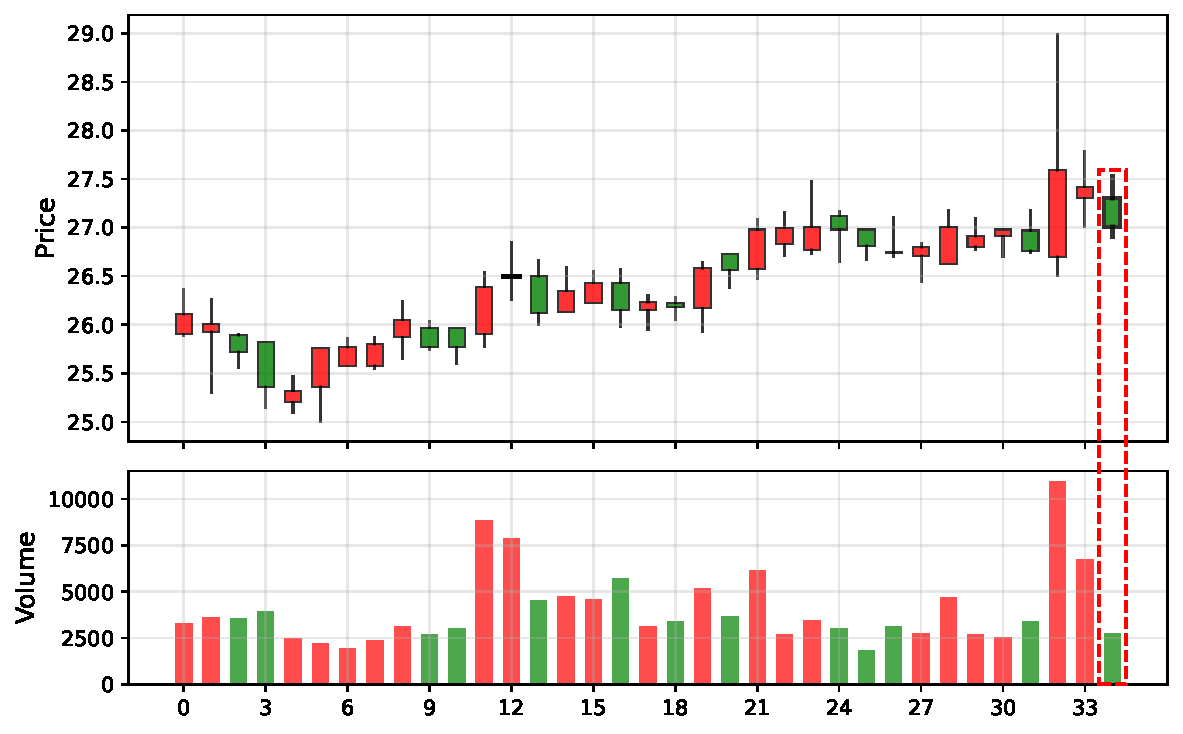
\includegraphics[width=0.32\textwidth]{tokens/original_kline.pdf}
        \caption{원본 토큰 시퀀스의 샘플.}
    \end{subfigure}

    \caption{토큰 사용 패턴의 시각화. 이 그림은 말뭉치에서의 출현 빈도를 기준으로 토큰 범주를 보여 준다: (a) 고빈도, (b) 저빈도, (c) 미사용(빈도 0) 토큰. 참고를 위해 원본 시퀀스 (d)의 샘플도 제시한다. (a), (b), (c)의 시퀀스는 (d)의 마지막 토큰을 해당 범주에서 무작위로 샘플링한 토큰으로 대체하여 구성하였다. 시각화에서 캔들스틱은 ``상승은 빨간색, 하락은 초록색'' 관례를 따르며(상승/하락은 시가 대비 종가로 결정됨), 거래량 막대도 이에 맞추어 색칠된다.}
    \label{fig:token_show_case}
\end{figure*}



\begin{figure*}[htbp]
    \centering

    \begin{subfigure}{\textwidth}
        \centering
        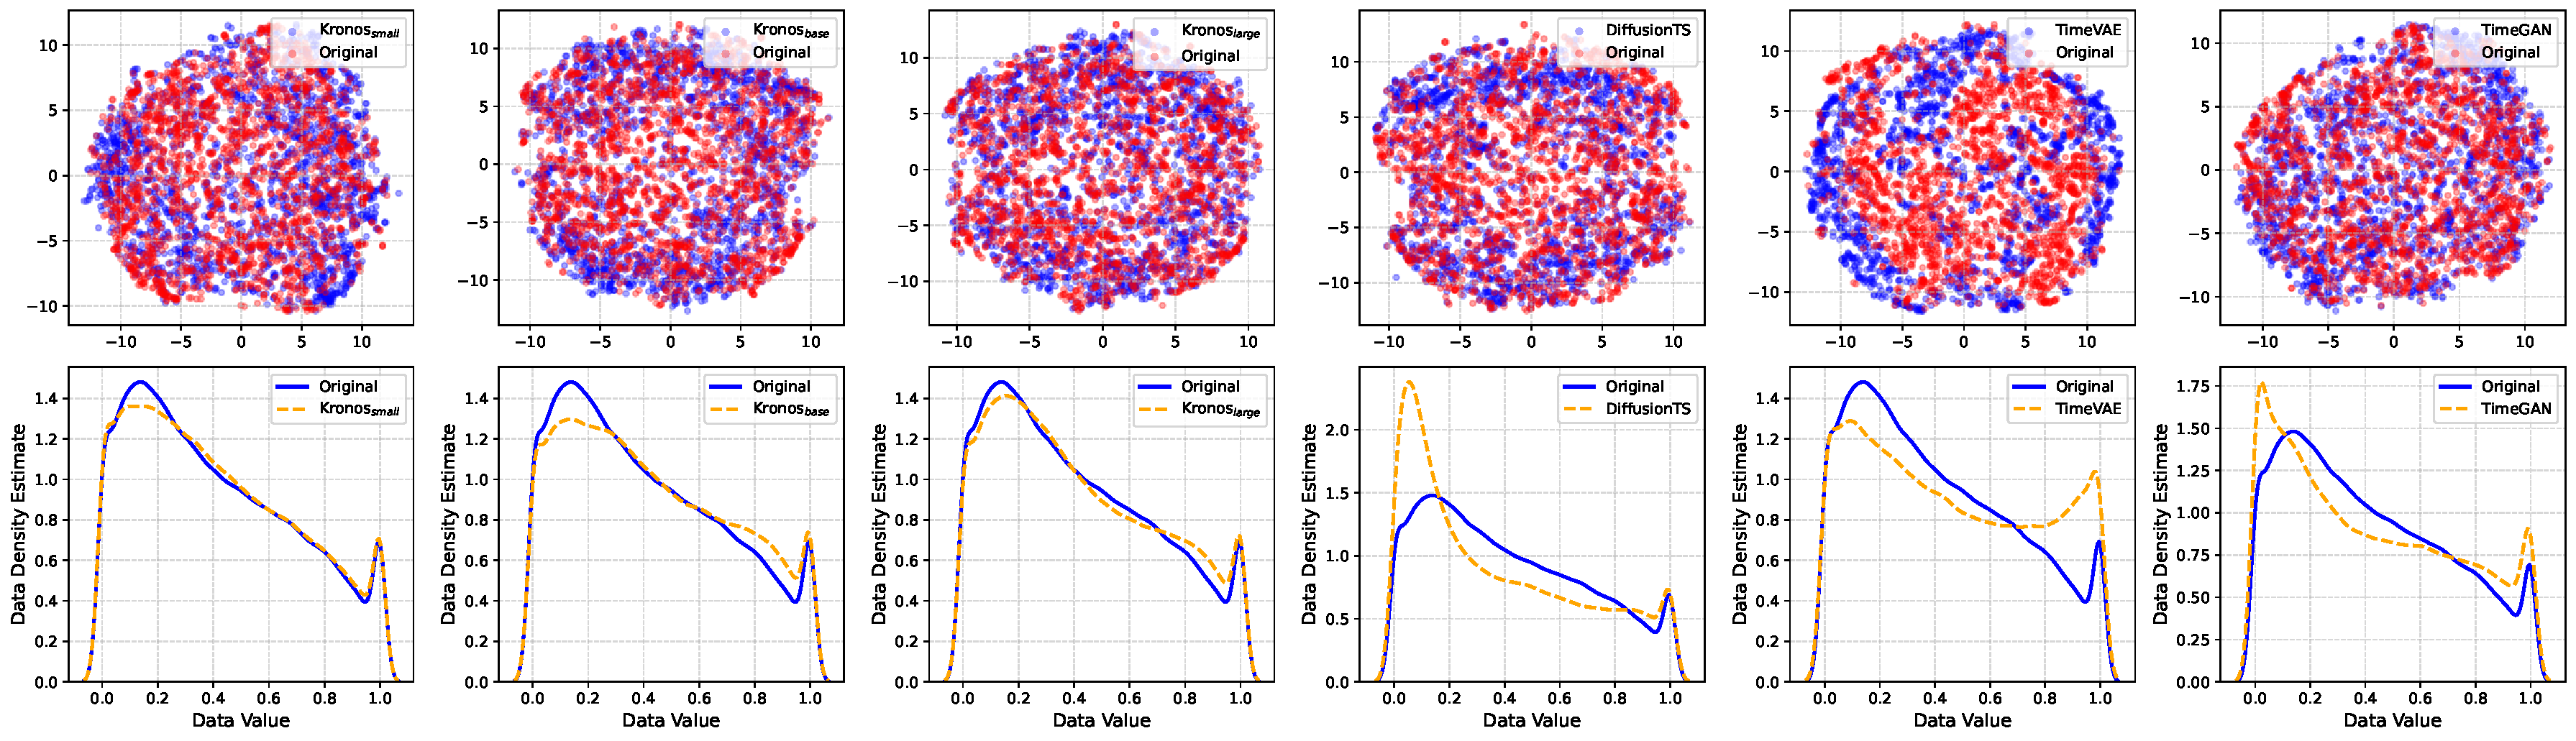
\includegraphics[width=1.0\textwidth]{img/gen_diversity_XSHG_daily.pdf}
        \caption{Shanghai Stock Exchange (XSHG), 일간 빈도}
    \end{subfigure}

    \begin{subfigure}{\textwidth}
        \centering
        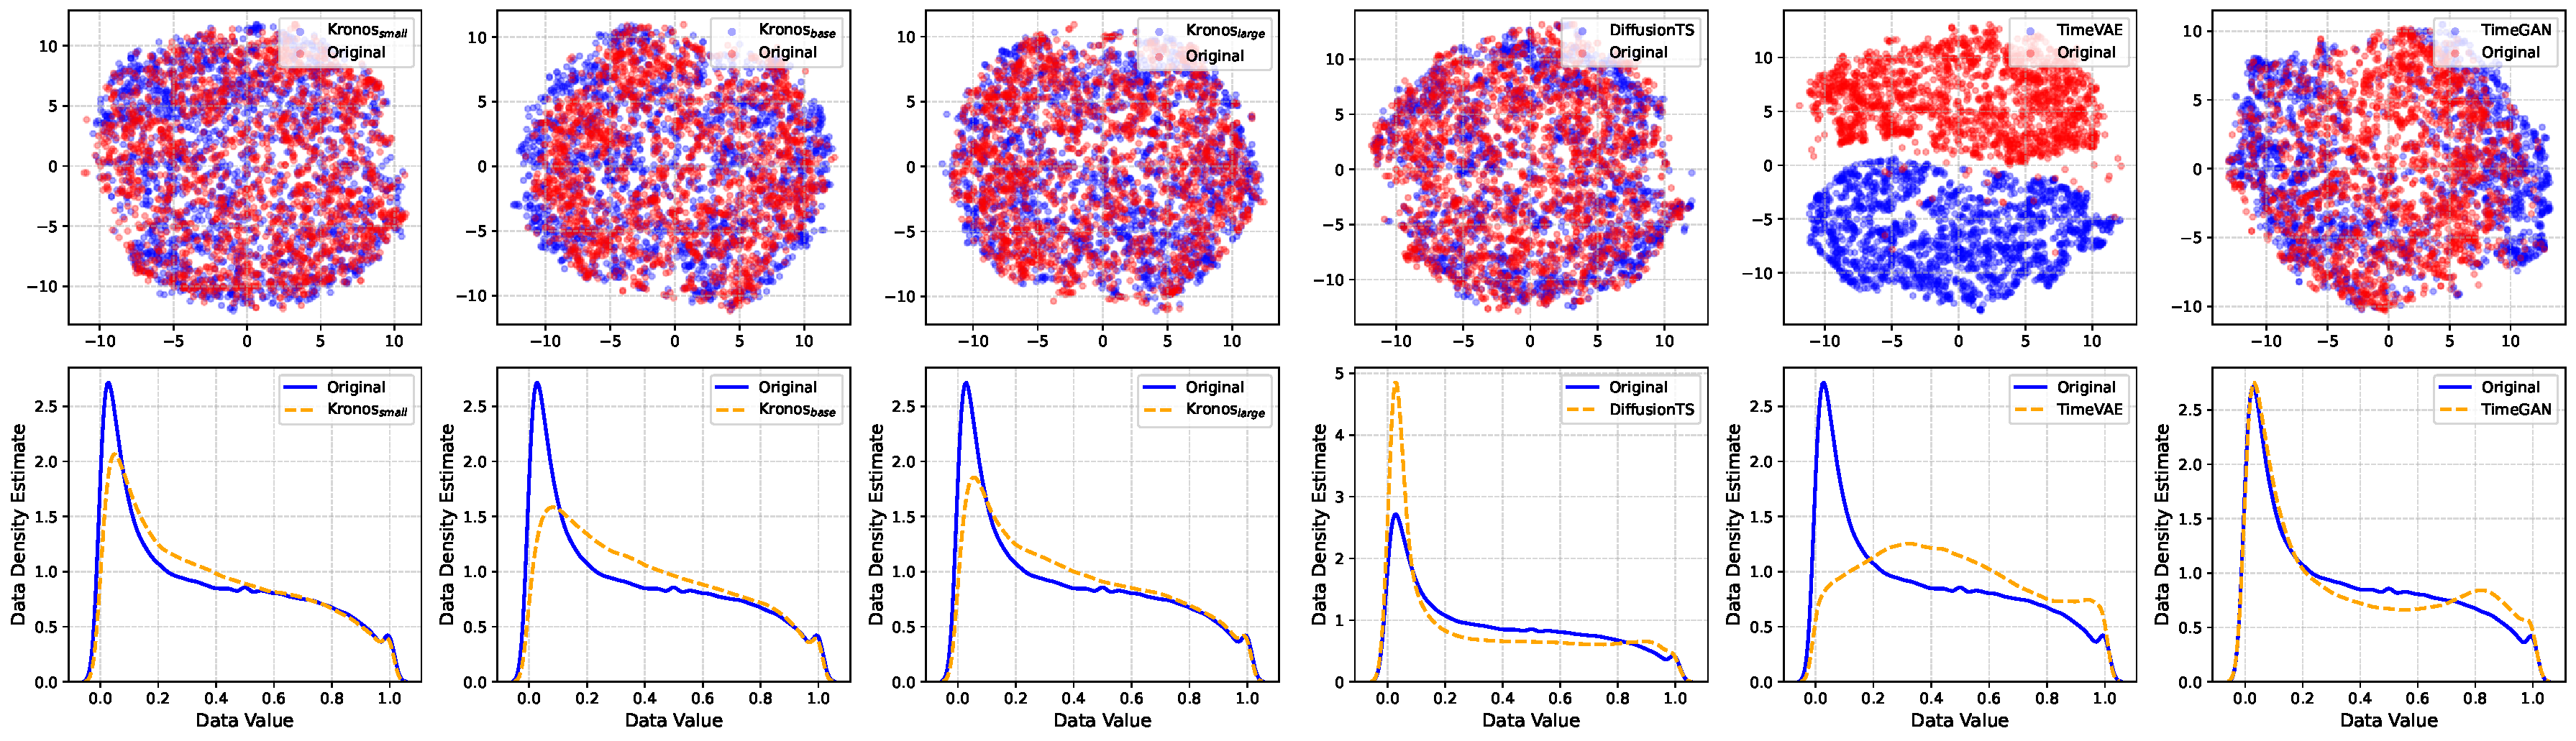
\includegraphics[width=1.0\textwidth]{img/gen_diversity_XTAI_15min.pdf}
        \caption{Taiwan Stock Exchange (XTAI), 15분 빈도}
    \end{subfigure}

    \begin{subfigure}{\textwidth}
        \centering
        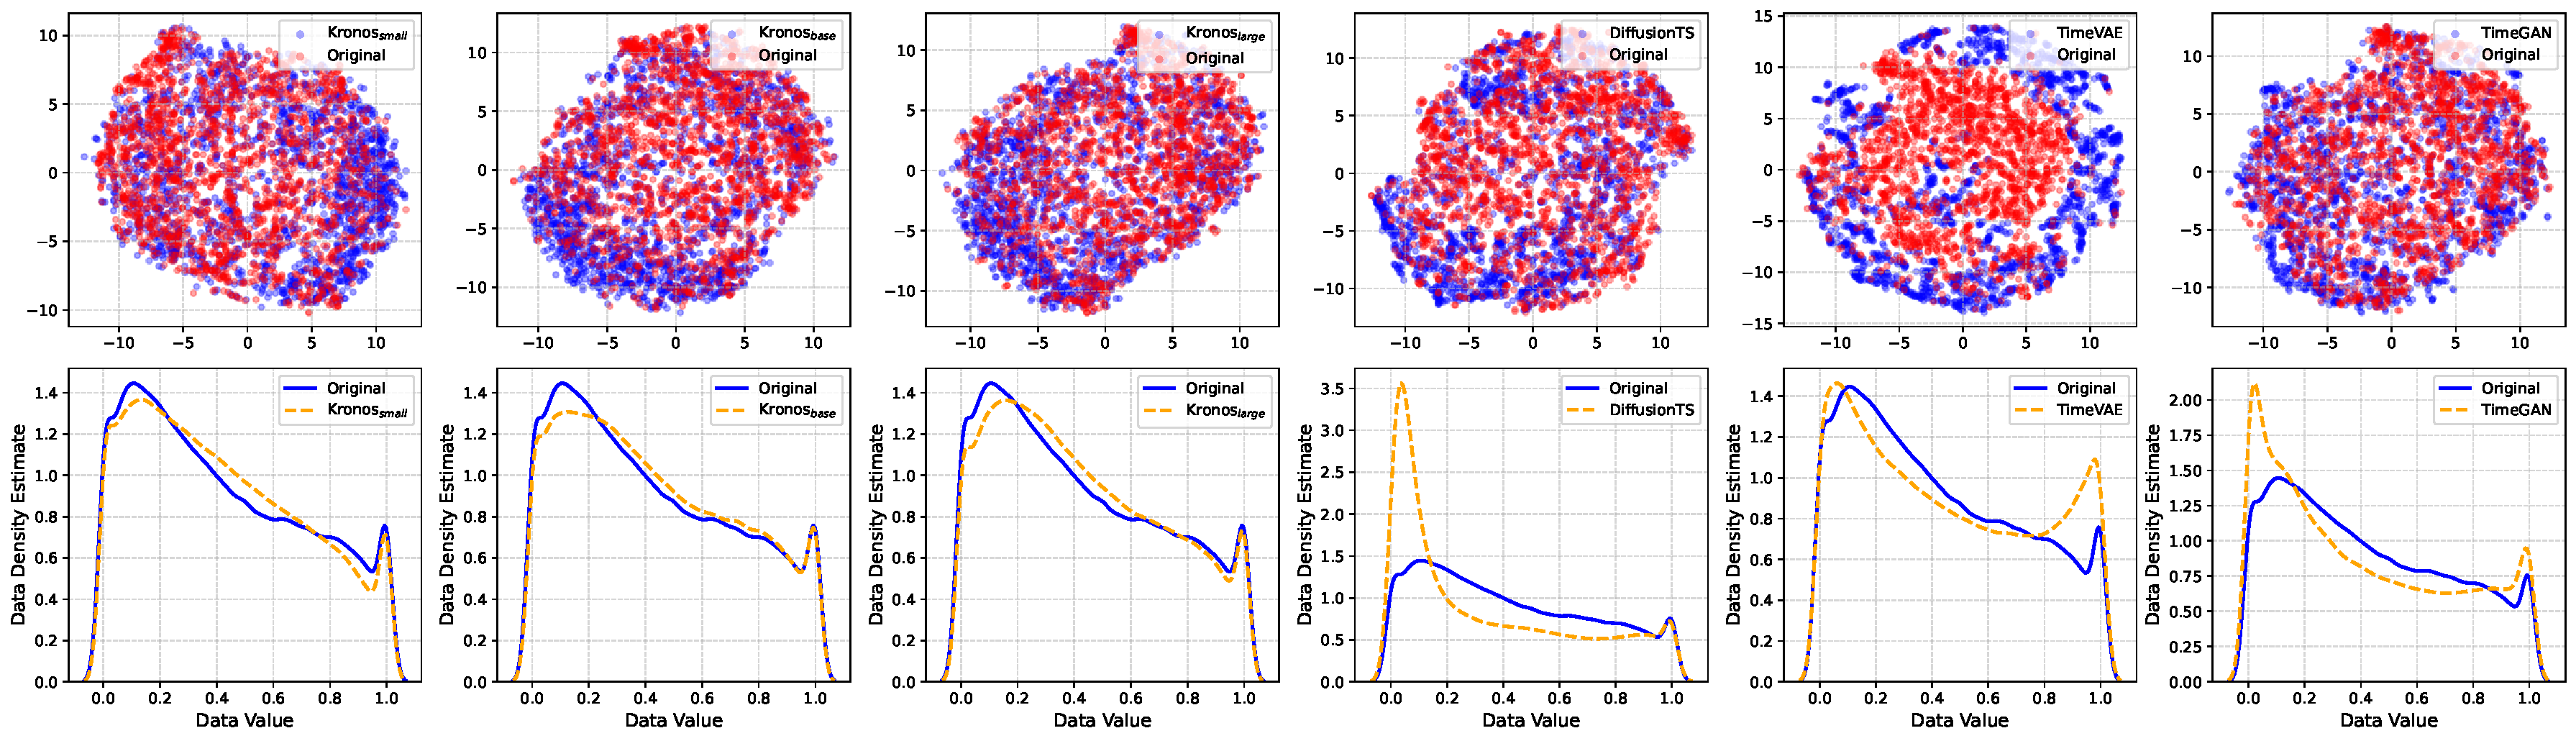
\includegraphics[width=1.0\textwidth]{img/gen_diversity_XTAI_daily.pdf}
        \caption{Taiwan Stock Exchange (XTAI), 일간 빈도}
    \end{subfigure}

    \begin{subfigure}{\textwidth}
        \centering
        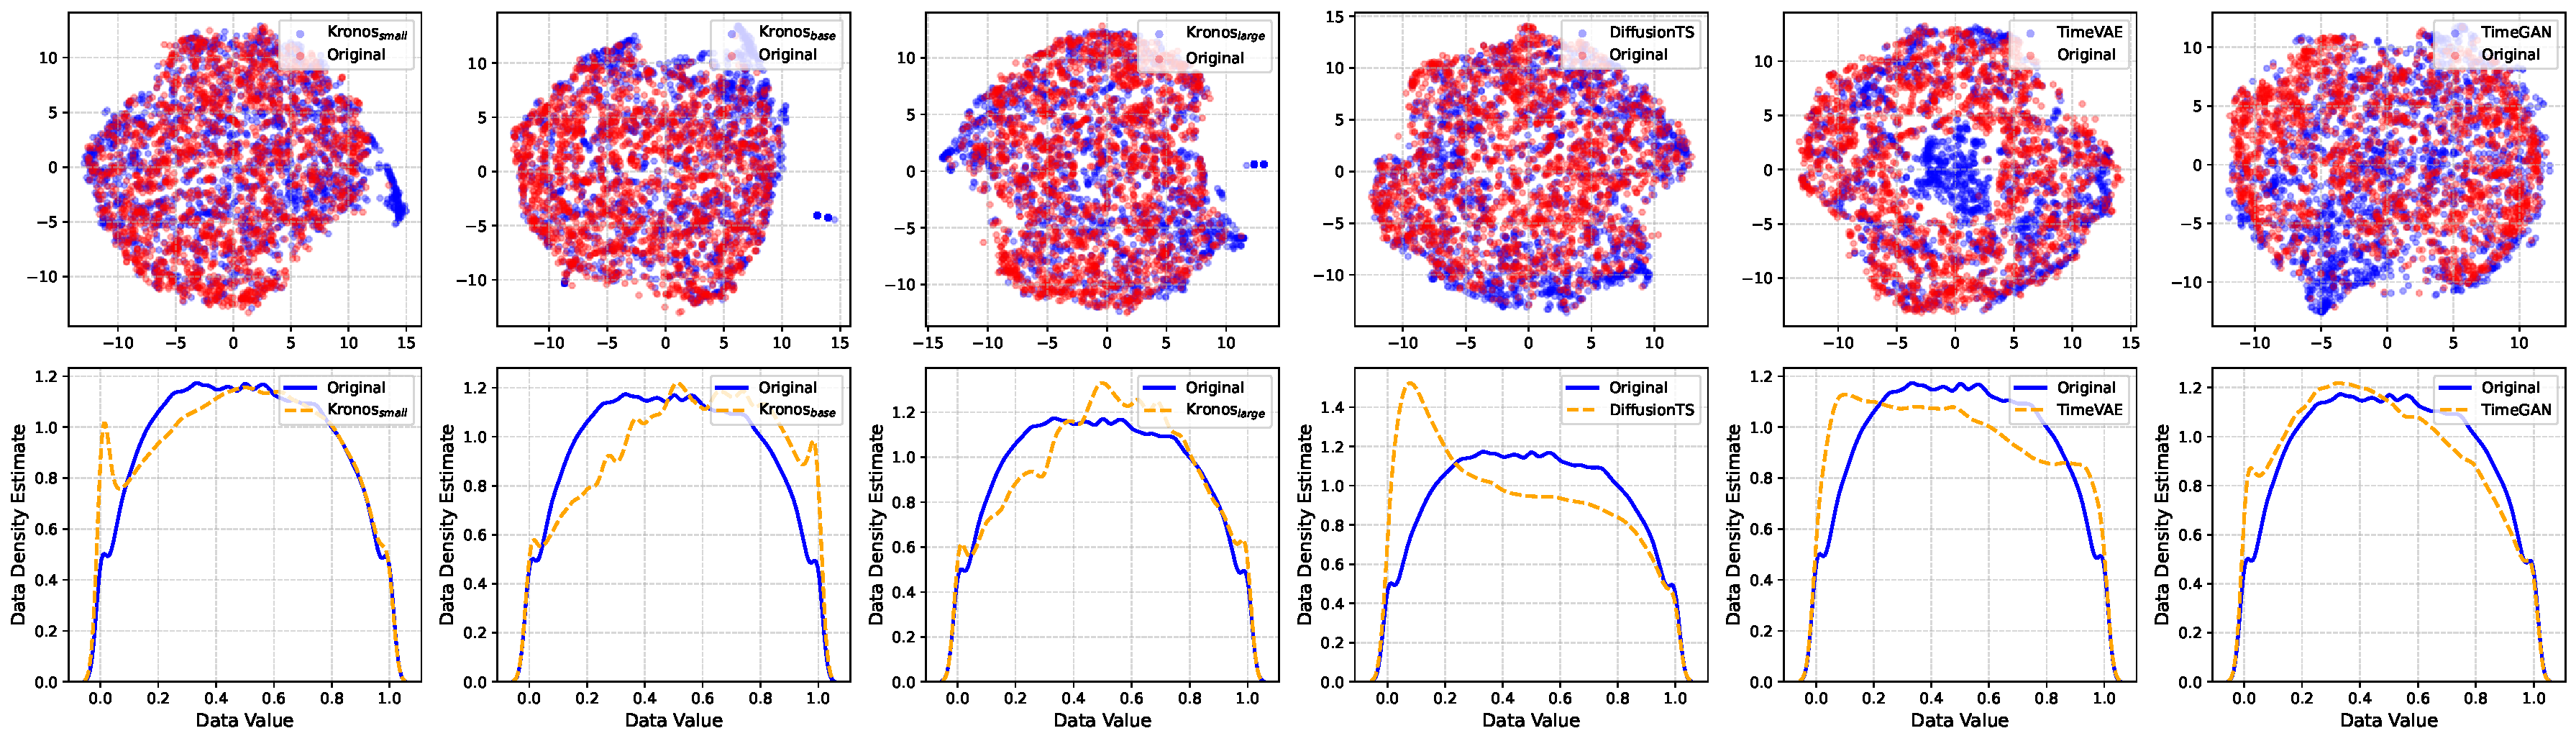
\includegraphics[width=1.0\textwidth]{img/gen_diversity_crypto_15min.pdf}
        \caption{암호화폐 (Crypto), 15분 빈도}
    \end{subfigure}

    \caption{
    서로 다른 데이터셋에서 생성 모델의 시각적 비교.
    \textbf{각 하위 그림의 위 행:} 원본 (\textcolor{red}{red}) 데이터와 합성 (\textcolor{blue}{blue}) 데이터의 t-SNE 임베딩.
    \textbf{각 하위 그림의 아래 행:} 원본 데이터와 합성 데이터의 커널 밀도 추정(KDE).}
    \label{fig:gen_visual_1}
\end{figure*}

\begin{figure*}[htbp]
    \centering

    % \captionsetup{labelformat=empty}

    \begin{subfigure}{\textwidth}
        \centering
        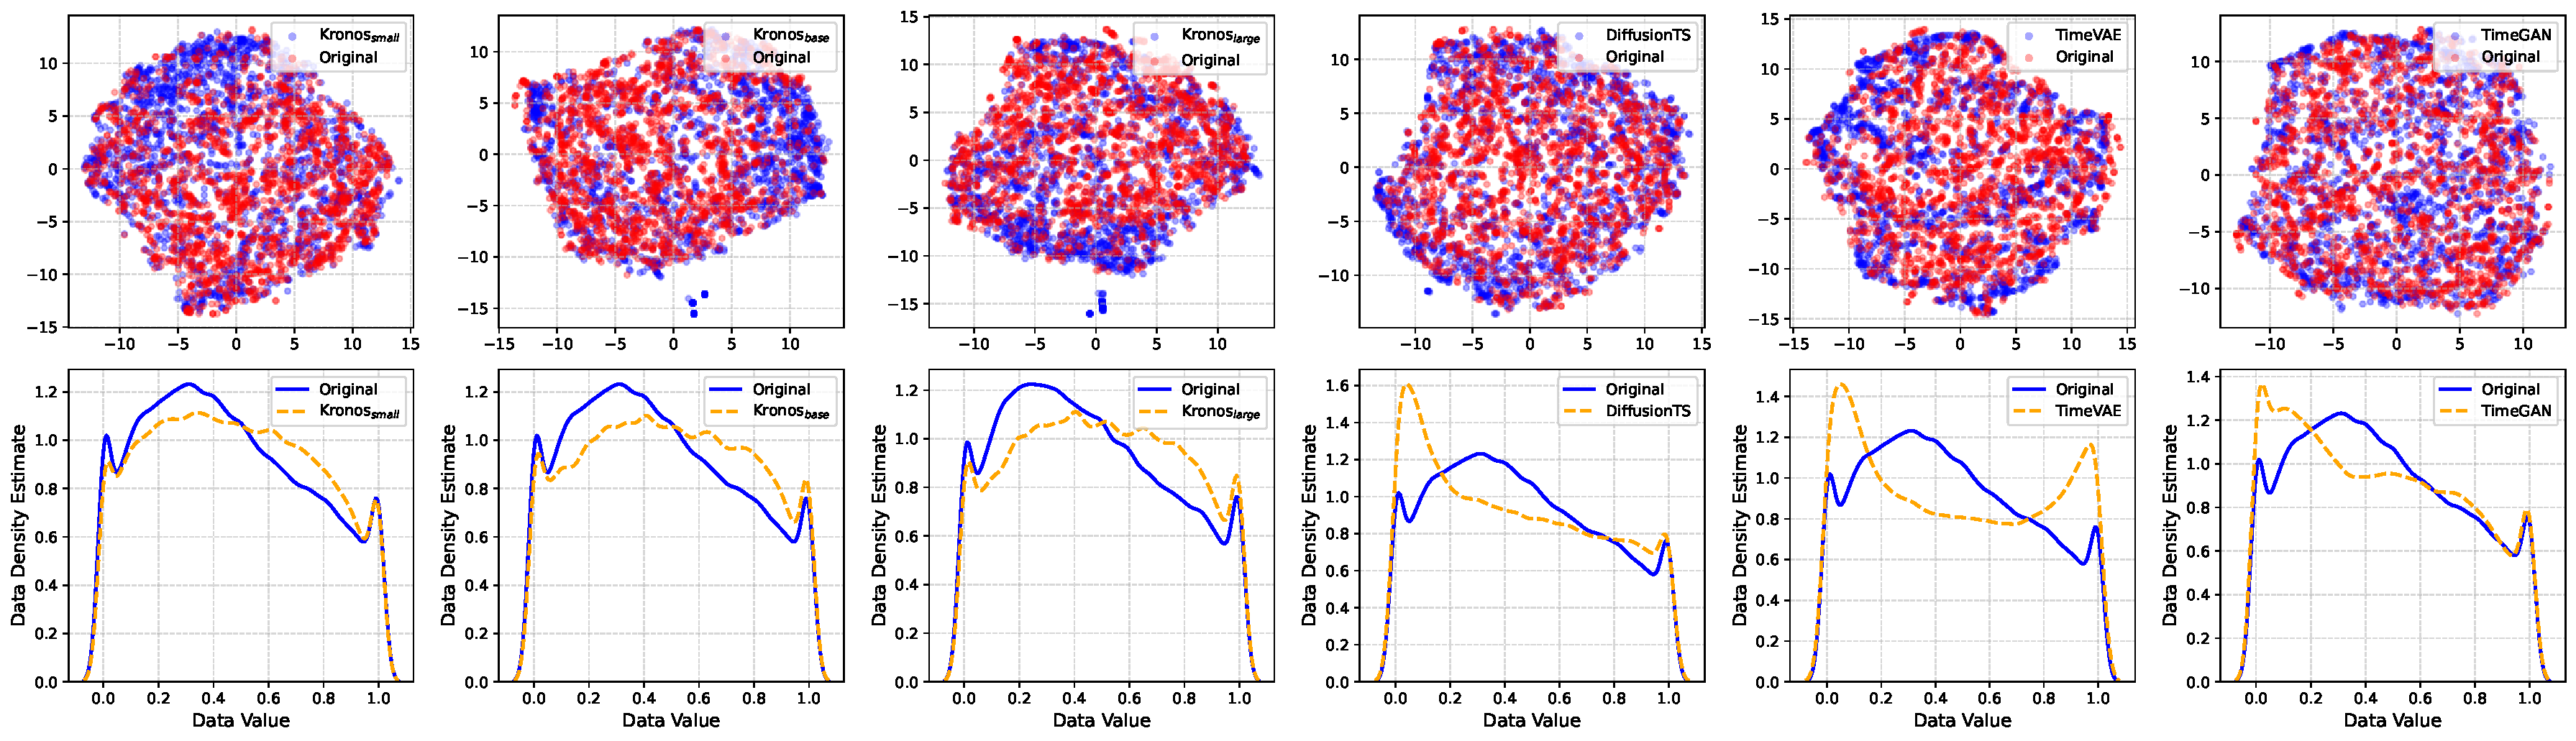
\includegraphics[width=1.0\textwidth]{img/gen_diversity_crypto_daily.pdf}
        \caption{암호화폐 (Crypto), 일간 빈도}
    \end{subfigure}

    \begin{subfigure}{\textwidth}
        \centering
        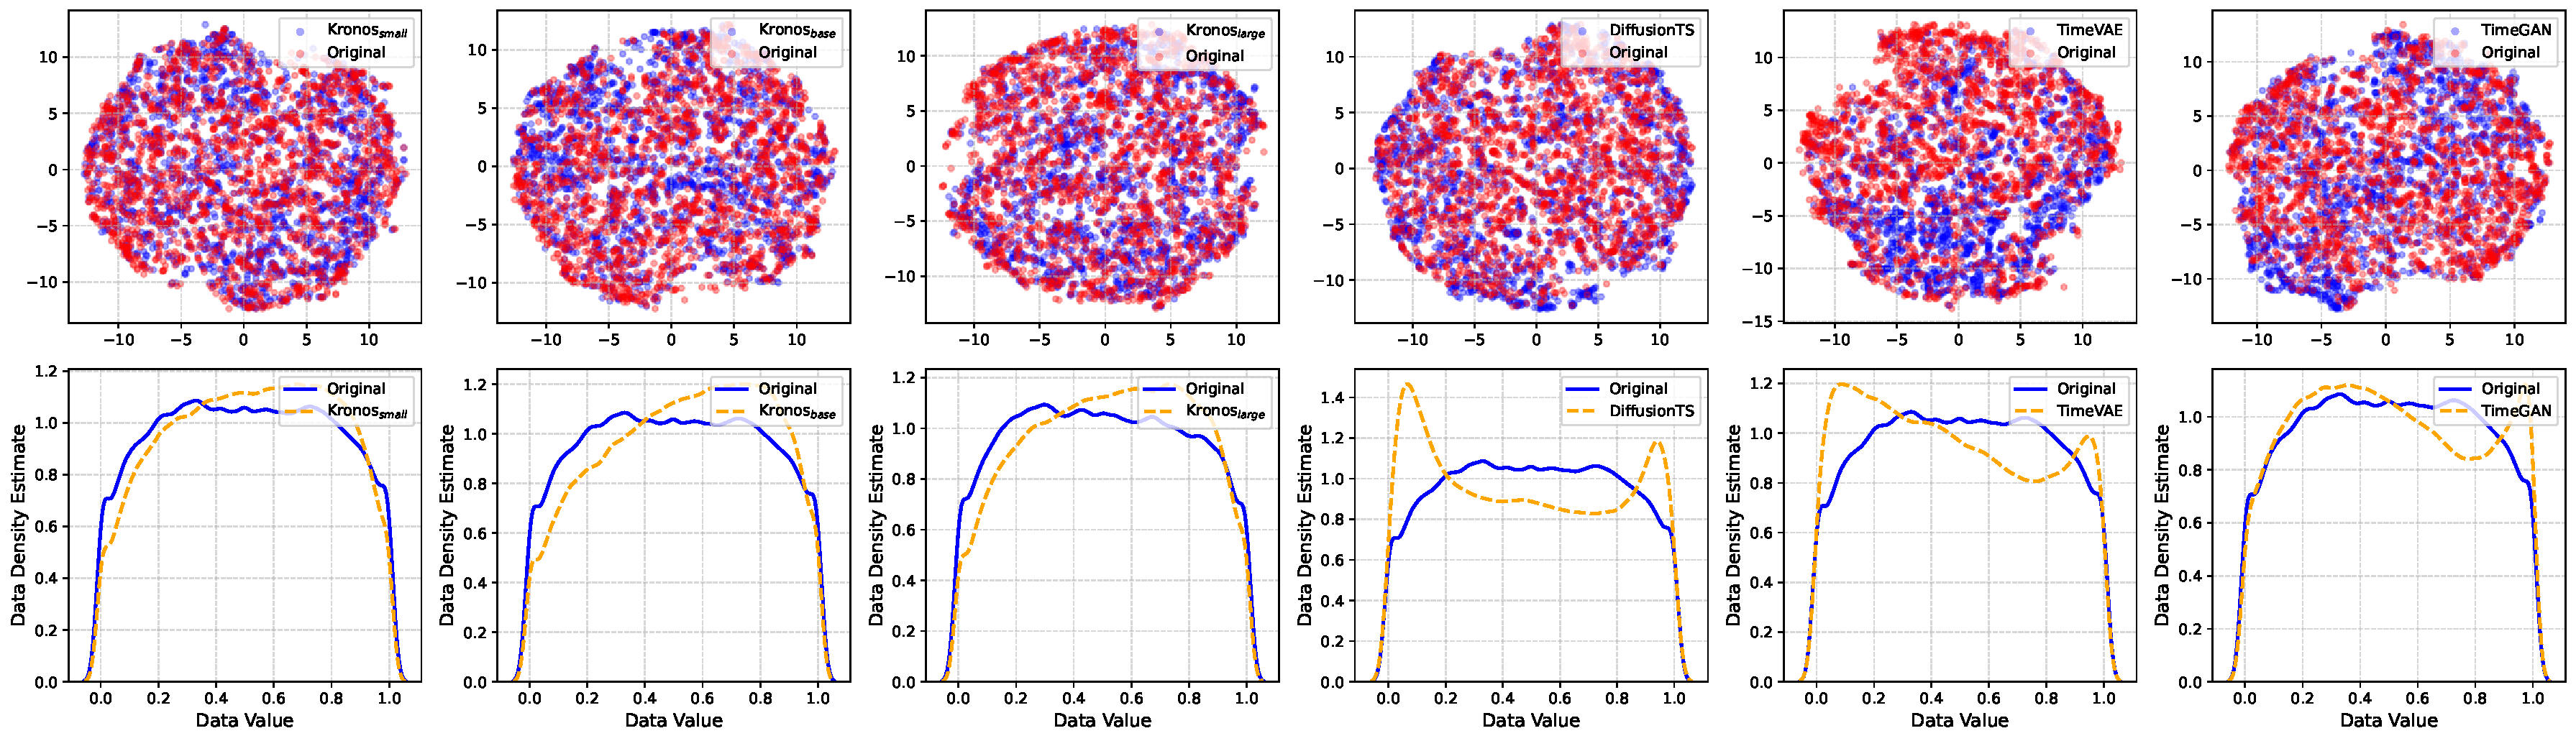
\includegraphics[width=1.0\textwidth]{img/gen_diversity_forex_15min.pdf}
        \caption{외환 (Forex), 15분 빈도}
    \end{subfigure}

    \begin{subfigure}{\textwidth}
        \centering
        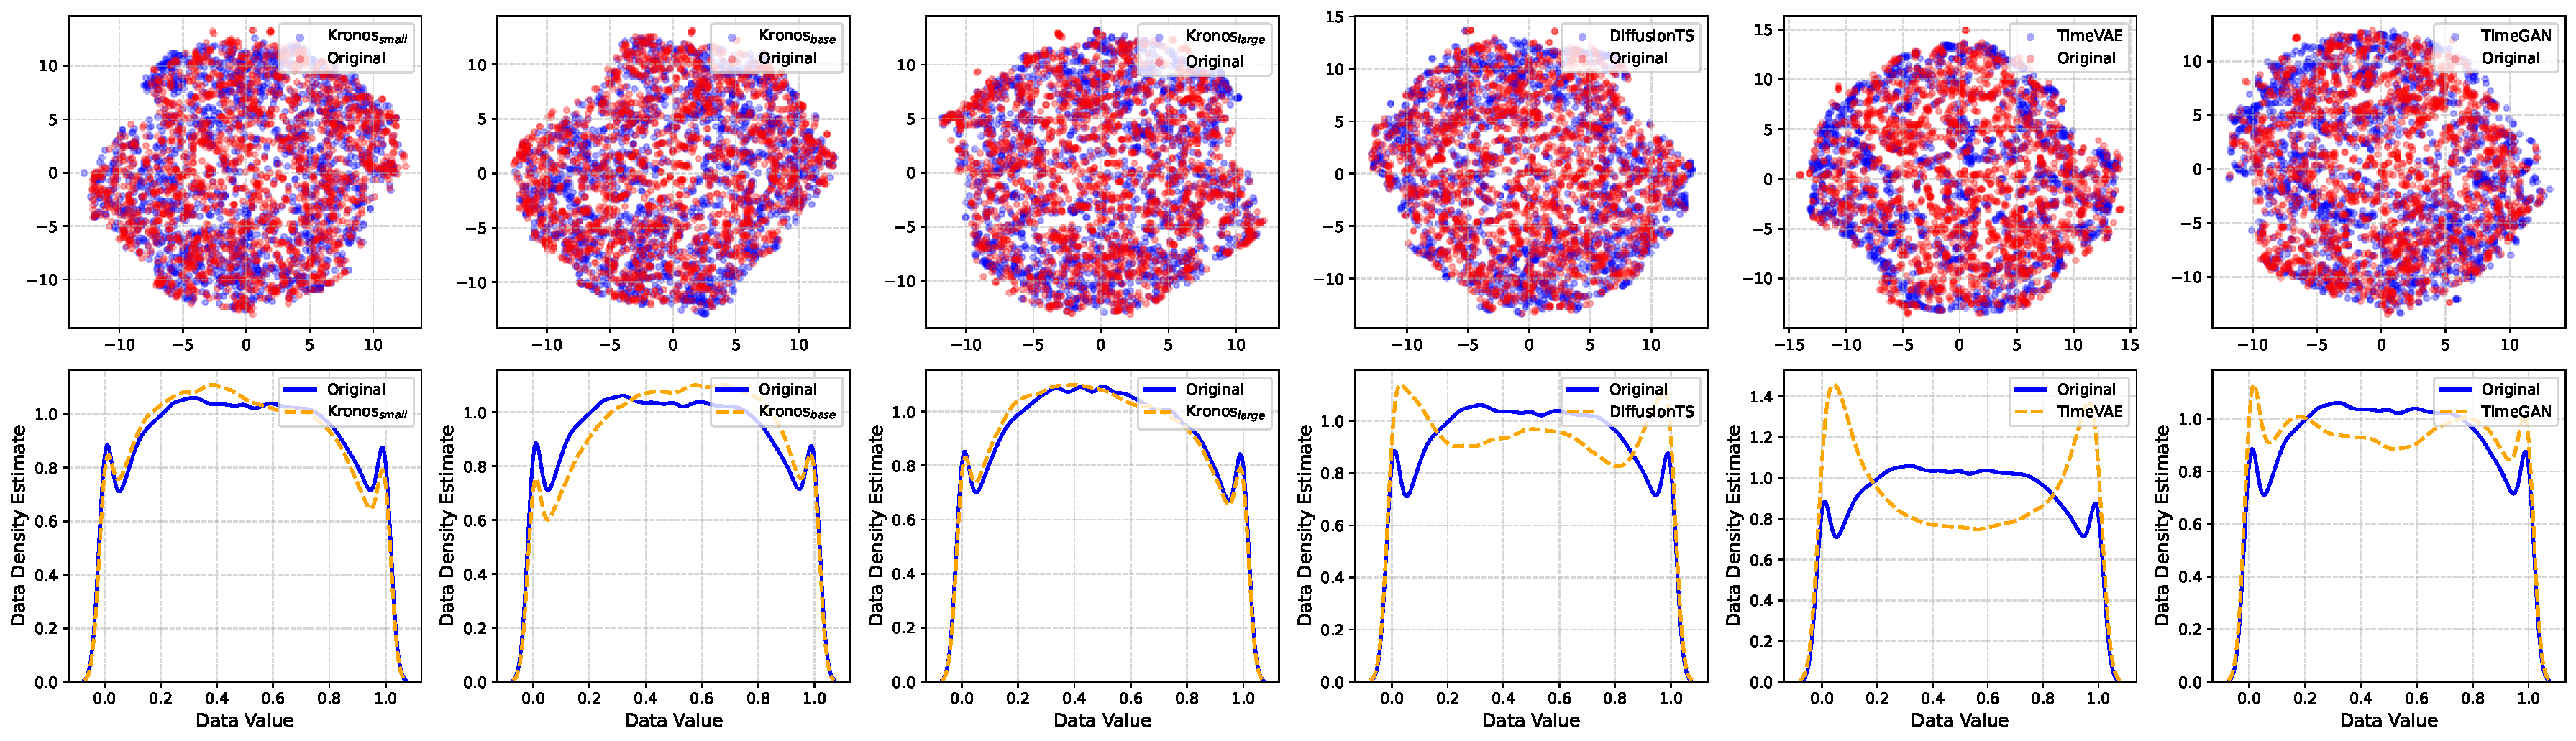
\includegraphics[width=1.0\textwidth]{img/gen_diversity_forex_daily.pdf}
        \caption{외환 (Forex), 일간 빈도}
    \end{subfigure}


    \caption{서로 다른 데이터셋에서 생성 모델의 시각적 비교.
    \textbf{각 하위 그림의 위 행:} 원본 (\textcolor{red}{red}) 데이터와 합성 (\textcolor{blue}{blue}) 데이터의 t-SNE 임베딩.
    \textbf{각 하위 그림의 아래 행:} 원본 데이터와 합성 데이터의 커널 밀도 추정(KDE).}
    \label{fig:gen_visual_2}
\end{figure*}




\begin{table*}[t]
  \centering
  \footnotesize
  \setlength{\tabcolsep}{4pt}

  \adjustbox{max width=\textwidth}{
  \begin{tabular}{l|c|*{11}{S}}
    \toprule
    \multicolumn{2}{c}{\textbf{모델}} &
    \multicolumn{3}{c}{\textbf{
\includegraphics[height=0.25cm]{img/logo_paper.png}\hspace{0.2em}Kronos (Ours)}} &
    \multicolumn{8}{c}{\textbf{Full-shot 시계열 모델}}\\
    \cmidrule(lr){3-5} \cmidrule(lr){6-13}
    \multicolumn{2}{c}{\textbf{지표}} &
    \textbf{$\text{Kronos}_S$} & \textbf{$\text{Kronos}_B$} & \textbf{$\text{Kronos}_L$} &
    \textbf{TimeXer} & \textbf{TimeMixer} & \textbf{iTransformer} & \textbf{PatchTST} &
    \textbf{TimesNet} & \textbf{DLinear} & \textbf{FEDformer} & \textbf{NSTransformer} \\
    \midrule

        \multirow{2}{*}{XSHG} & IC     & \best{0.0549} & \second{0.0564} & 0.0546 & 0.0280 & 0.0291 & 0.0350 & 0.0450 & 0.0424 & 0.0405 & 0.0233 & 0.0433 \\
                              & RankIC & 0.0375 & \best{0.0390} & \second{0.0381} & 0.0053 & 0.0079 & 0.0128 & 0.0088 & 0.0175 & 0.0181 & 0.0107 & 0.0155 \\
        \midrule
        \multirow{2}{*}{XNAS} & IC     & \second{0.0343} & 0.0322 & \best{0.0361} & 0.0132 & 0.0097 & 0.0204 & 0.0116 & 0.0174 & 0.0197 & 0.0165 & 0.0253 \\
                              & RankIC & 0.0155 & \second{0.0190} & \best{0.0191} & 0.0106 & 0.0048 & 0.0111 & 0.0083 & 0.0084 & 0.0084 & -0.0014 & 0.0016 \\
        \midrule
        \multirow{2}{*}{XJPX} & IC     & 0.0314 & \second{0.0332} & \best{0.0360} & 0.0094 & 0.0017 & 0.0137 & 0.0053 & 0.0099 & 0.0118 & 0.0046 & 0.0281 \\
                              & RankIC & 0.0199 & 0.0209 & \best{0.0277} & 0.0159 & 0.0036 & \second{0.0271} & 0.0056 & 0.0127 & 0.0149 & 0.0024 & 0.0212 \\
        \midrule
        \multirow{2}{*}{XNSE} & IC     & \second{0.0634} & \best{0.0648} & \second{0.0634} & -0.0055 & 0.0094 & -0.0252 & 0.0082 & 0.0566 & 0.0024 & 0.0063 & 0.0514 \\
                              & RankIC & 0.0434 & \second{0.0464} & \best{0.0486} & -0.0371 & 0.0024 & -0.0248 & 0.0084 & 0.0379 & -0.0024 & 0.0003 & 0.0225 \\
        \midrule
        \multirow{2}{*}{XKRX} & IC     & 0.0550 & \best{0.0575} & \second{0.0567} & -0.0328 & 0.0036 & -0.0442 & 0.0248 & 0.0416 & 0.0001 & -0.0070 & 0.0416 \\
                              & RankIC & 0.0362 & \best{0.0393} & \second{0.0373} & -0.0160 & 0.0033 & -0.0284 & 0.0214 & 0.0285 & 0.0006 & -0.0049 & 0.0058 \\
        \midrule
        \multirow{2}{*}{XHKG} & IC     & \second{0.0435} & \best{0.0439} & 0.0428 & 0.0318 & 0.0322 & 0.0336 & 0.0401 & 0.0333 & 0.0392 & 0.0296 & 0.0366 \\
                              & RankIC & 0.0226 & \best{0.0236} & \second{0.0228} & -0.0051 & -0.0009 & -0.0021 & -0.0068 & -0.0040 & -0.0009 & -0.0078 & -0.0017 \\
        \midrule
        \multirow{2}{*}{XIDX} & IC     & \second{0.0551} & \second{0.0551} & \best{0.0573} & -0.0139 & 0.0116 & -0.0233 & 0.0194 & 0.0468 & 0.0158 & 0.0169 & 0.0381 \\
                              & RankIC & 0.0214 & \second{0.0216} & \best{0.0223} & 0.0025 & 0.0046 & 0.0011 & 0.0149 & 0.0171 & 0.0037 & 0.0084 & 0.0051 \\
        \midrule
        \multirow{2}{*}{XKLS} & IC     & \second{0.0411} & 0.0408 & \best{0.0466} & -0.0283 & 0.0079 & -0.0281 & -0.0037 & 0.0341 & 0.0306 & -0.0102 & 0.0101 \\
                              & RankIC & \best{0.0215} & 0.0149 & 0.0167 & 0.0051 & 0.0171 & 0.0024 & -0.0078 & -0.0025 & \second{0.0208} & -0.0169 & -0.0103 \\
        \midrule
        \multirow{2}{*}{XTAI} & IC     & 0.0424 & \second{0.0443} & \best{0.0448} & 0.0282 & 0.0197 & 0.0275 & 0.0328 & 0.0312 & 0.0394 & 0.0249 & 0.0334 \\
                              & RankIC & 0.0301 & \second{0.0320} & \best{0.0342} & -0.0042 & 0.0015 & 0.0111 & 0.0147 & 0.0095 & 0.0192 & 0.0059 & 0.0129 \\
        \midrule
        \multirow{2}{*}{Crypto} & IC     & \best{0.0247} & 0.0209 & \second{0.0211}  & 0.0105 & 0.0128 & 0.0155 & 0.0149 & 0.0192 & 0.0137 & 0.0081 & 0.0164 \\
                                & RankIC & 0.0138 & 0.0135 & 0.0129  & 0.0022 & 0.0038 & 0.0134 & \best{0.0192} & \second{0.0146} & 0.0040 & 0.0000 & 0.0096\\
        \midrule
        \multirow{2}{*}{Forex} & IC     & \second{0.0279} & \best{0.0292} & 0.0244 & 0.0124 & 0.0102 & 0.0142 & 0.0158 & 0.0167 & 0.0227 & 0.0153 & 0.0228 \\
                               & RankIC & \best{0.0177} & 0.0141 & 0.0137 & 0.0134 & 0.0128 & 0.0090 & 0.0085 & \second{0.0175} & 0.0168 & 0.0120 & 0.0079 \\
        \midrule

        \rowcolor{AvgGray}
          & IC &
        0.0431 & \second{0.0435} & \best{0.0440} & 0.0048 & 0.0134 & 0.0036 & 0.0195 & 0.0317 & 0.0214 & 0.0117 & 0.0316 \\
        \rowcolor{AvgGray} \multirow{2}{*}[2.5ex]{\textbf{평균}} & RankIC &
        0.0254 & \second{0.0258} & \best{0.0267} & -0.0007 & 0.0055 & 0.0030 & 0.0087 & 0.0143 & 0.0094 & 0.0008 & 0.0082 \\
         \midrule
    \rowcolor{CntGray}
    \multicolumn{2}{c}{\textbf{$\mathbf{1^{st}}$ 횟수}} &
\cnt{4} & \cnt{7} & \cnt{10} & \cnt{0} & \cnt{0} & \cnt{0} &
\cnt{1} & \cnt{0} & \cnt{0} & \cnt{0} & \cnt{0} \\
    \bottomrule
  \end{tabular}}
  \caption{가격 시계열 예측 실험의 전체 결과(Part 1): 우리 모델(Kronos) 및 full-shot 시계열 모델. IC 또는 RankIC가 높을수록 더 나은 예측을 의미한다. 최고 및 차상위 결과는 각각 \best{빨간 밑줄}과 \second{파란 밑줄}로 표시하였다.}
  \label{tab:full_price_forecasting_1}
\end{table*}

\begin{table*}[t]
    \centering
    \footnotesize
    \setlength{\tabcolsep}{4pt}


    \adjustbox{max width=\textwidth}{
    \begin{tabular}{l|c|*{13}{S}}
        \toprule
        \multicolumn{2}{c}{\textbf{모델}} &
        \multicolumn{12}{c}{\textbf{Zero-shot 시계열 모델}} \\
        \cmidrule(lr){3-14}
        \multicolumn{2}{c}{\textbf{지표}} &
        \textbf{$\text{Time\text{-}MOE}_{S}$} & \textbf{$\text{Time\text{-}MOE}_{B}$} &
        \textbf{$\text{Moirai}_{S}$} & \textbf{$\text{Moirai}_{B}$} & \textbf{$\text{Moirai}_{L}$} &
        \textbf{TimesFM} &
        \textbf{$\text{Moment}_{S}$} & \textbf{$\text{Moment}_{B}$} & \textbf{$\text{Moment}_{L}$} &
        \textbf{$\text{Chronos}_{S}$} & \textbf{$\text{Chronos}_{B}$} & \textbf{$\text{Chronos}_{L}$} \\
        \midrule
        \multirow{2}{*}{XSHG} & IC     & 0.0463 & 0.0493 & -0.0007 & -0.0005 & -0.0002 & 0.0174 & 0.0028 & -0.0032 & -0.0009 & 0.0147 & 0.0069 & 0.0195 \\
                              & RankIC & 0.0304 & 0.0317 & 0.0000 & -0.0012 & 0.0003 & 0.0020 & 0.0003 & -0.0037 & -0.0017 & -0.0026 & -0.0108 & 0.0025 \\
        \midrule
        \multirow{2}{*}{XNAS} & IC     & -0.0032 & -0.0045 & -0.0008 & -0.0005 & 0.0000 & 0.0076 & 0.0010 & -0.0023 & -0.0003 & -0.0025 & -0.0005 & 0.0020 \\
                              & RankIC & -0.0033 & -0.0042 & -0.0008 & 0.0013 & 0.0007 & 0.0112 & -0.0015 & -0.0027 & -0.0007 & -0.0001 & 0.0008 & 0.0030 \\
        \midrule
        \multirow{2}{*}{XJPX} & IC     & 0.0268 & 0.0280 & 0.0012 & 0.0004 & 0.0000 & 0.0076 & -0.0010 & -0.0003 & -0.0027 & 0.0117 & 0.0113 & 0.0067 \\
                              & RankIC & 0.0228 & 0.0230 & 0.0025 & 0.0019 & 0.0016 & 0.0073 & -0.0031 & 0.0010 & -0.0006 & 0.0110 & 0.0123 & 0.0070 \\
        \midrule
        \multirow{2}{*}{XNSE} & IC     & 0.0173 & 0.0190 & -0.0005 & -0.0008 & -0.0006 & 0.0025 & 0.0063 & -0.0129 & -0.0039 & -0.0012 & -0.0049 & 0.0014 \\
                              & RankIC & 0.0155 & 0.0169 & -0.0021 & -0.0021 & -0.0029 & 0.0009 & 0.0060 & -0.0104 & -0.0055 & -0.0041 & -0.0066 & -0.0005 \\
        \midrule
        \multirow{2}{*}{XKRX} & IC     & 0.0113 & 0.0141 & -0.0014 & 0.0006 & -0.0011 & -0.0105 & 0.0056 & -0.0083 & -0.0114 & -0.0009 & -0.0018 & 0.0061 \\
                              & RankIC & 0.0088 & 0.0118 & -0.0020 & 0.0006 & -0.0002 & -0.0097 & 0.0041 & -0.0082 & -0.0069 & -0.0006 & -0.0009 & 0.0072 \\
        \midrule
        \multirow{2}{*}{XHKG} & IC     & 0.0174 & 0.0189 & 0.0000 & -0.0001 & -0.0013 & 0.0117 & 0.0013 & -0.0050 & -0.0003 & 0.0159 & 0.0140 & 0.0166 \\
                              & RankIC & 0.0186 & 0.0201 & 0.0003 & 0.0031 & 0.0011 & 0.0058 & -0.0034 & -0.0013 & 0.0009 & 0.0190 & 0.0179 & 0.0192 \\
        \midrule
        \multirow{2}{*}{XIDX} & IC     & -0.0053 & -0.0052 & -0.0009 & -0.0009 & -0.0003 & 0.0026 & 0.0052 & -0.0094 & -0.0007 & 0.0021 & 0.0042 & 0.0080 \\
                              & RankIC & 0.0002 & 0.0000 & 0.0008 & 0.0012 & 0.0007 & 0.0042 & -0.0015 & -0.0029 & 0.0014 & 0.0087 & 0.0122 & 0.0153 \\
        \midrule
        \multirow{2}{*}{XKLS} & IC     & 0.0123 & 0.0125 & -0.0003 & -0.0028 & 0.0005 & 0.0106 & 0.0045 & -0.0093 & -0.0065 & -0.0080 & -0.0076 & -0.0077 \\
                              & RankIC & 0.0112 & 0.0135 & 0.0010 & 0.0027 & 0.0047 & -0.0052 & 0.0000 & 0.0017 & -0.0031 & 0.0113 & 0.0118 & 0.0114 \\
        \midrule
        \multirow{2}{*}{XTAI} & IC     & 0.0296 & 0.0292 & 0.0005 & 0.0001 & -0.0004 & -0.0002 & 0.0025 & -0.0047 & -0.0046 & 0.0028 & -0.0002 & 0.0080 \\
                              & RankIC & 0.0234 & 0.0224 & 0.0011 & 0.0013 & 0.0003 & -0.0028 & 0.0001 & -0.0023 & -0.0009 & 0.0088 & 0.0060 & 0.0125 \\
        \midrule
        \multirow{2}{*}{Crypto} & IC     & 0.0054 & 0.0037 & -0.0008 & -0.0006 & -0.0004 & -0.0009 & -0.0002 & -0.0004 & -0.0030 & -0.0114 & -0.0129 & -0.0096 \\
                                & RankIC & 0.0069 & 0.0050 & 0.0004 & 0.0011 & 0.0000 & 0.0014 & -0.0011 & -0.0061 & -0.0007 & -0.0051 & -0.0061 & -0.0045 \\
        \midrule
        \multirow{2}{*}{Forex} & IC     & 0.0265 & 0.0267 & -0.0011 & -0.0011 & 0.0000 & 0.0092 & -0.0007 & 0.0008 & 0.0024 & 0.0176 & 0.0143 & 0.0155 \\
                               & RankIC & 0.0115 & 0.0114 & -0.0010 & 0.0005 & -0.0003 & 0.0076 & -0.0014 & -0.0010 & 0.0022 & 0.0168 & 0.0147 & 0.0127 \\
        \midrule

        \rowcolor{AvgGray}
         & IC &
        0.0168 & 0.0174 & -0.0004 & -0.0006 & -0.0003 & 0.0052 & 0.0025 & -0.0050 & -0.0029 & 0.0037 & 0.0021 & 0.0060 \\
        \rowcolor{AvgGray} \multirow{2}{*}[2.5ex]{\textbf{평균}} & RankIC &
        0.0133 & 0.0138 & 0.0000 & 0.0009 & 0.0005 & 0.0021 & -0.0001 & -0.0033 & -0.0014 & 0.0057 & 0.0047 & 0.0078 \\
        \midrule
        \rowcolor{CntGray}
        \multicolumn{2}{c}{\textbf{$\mathbf{1^{st}}$ 횟수}} &
\cnt{0} & \cnt{0} & \cnt{0} & \cnt{0} & \cnt{0} & \cnt{0} &
\cnt{0} & \cnt{0} & \cnt{0} & \cnt{0} & \cnt{0} & \cnt{0} \\
        \bottomrule
    \end{tabular}}
\caption{가격 시계열 예측 실험의 전체 결과(Part 2): zero-shot 시계열 모델. IC 또는 RankIC가 높을수록 더 나은 예측을 의미한다. 최고 및 차상위 결과는 각각 \best{빨간 밑줄}과 \second{파란 밑줄}로 표시하였다.}
    \label{tab:full_price_forecasting_2}
\end{table*}

\begin{table*}[t]
  \centering
  \footnotesize
  \setlength{\tabcolsep}{4pt}

  \adjustbox{max width=\textwidth}{
  \begin{tabular}{l|c|*{11}{S}}
    \toprule
    \multicolumn{2}{c}{\textbf{모델}} &
    \multicolumn{3}{c}{\textbf{
\includegraphics[height=0.25cm]{img/logo_paper.png}\hspace{0.2em}Kronos (Ours)}} &
    \multicolumn{8}{c}{\textbf{Full-shot 시계열 모델}}\\
    \cmidrule(lr){3-5} \cmidrule(lr){6-13}
    \multicolumn{2}{c}{\textbf{지표}} &
    \textbf{$\text{Kronos}_S$} & \textbf{$\text{Kronos}_B$} & \textbf{$\text{Kronos}_L$} &
    \textbf{TimeXer} & \textbf{TimeMixer} & \textbf{iTransformer} & \textbf{PatchTST} &
    \textbf{TimesNet} & \textbf{DLinear} & \textbf{FEDformer} & \textbf{NSTransformer}\\
    \midrule

        % ------------------- 데이터 영역 업데이트됨 -------------------
        \multirow{2}{*}{XSHG} & IC     & \second{0.0677} & 0.0652 & 0.0662 & 0.0456 & 0.0114 & 0.0371 & 0.0467 & 0.0563 & 0.0626 & 0.0589 & \best{0.0777} \\
                              & RankIC & 0.0617 & 0.0653 & 0.0642 & 0.0306 & -0.0072 & 0.0266 & 0.0437 & 0.0421 & 0.0461 & 0.0568 & 0.0595 \\
        \midrule
        \multirow{2}{*}{XNAS} & IC     & 0.0563 & \second{0.0626} & \best{0.0639} & 0.0051 & 0.0270 & 0.0340 & 0.0569 & -0.0193 & 0.0144 & 0.0219 & 0.0377 \\
                              & RankIC & 0.0513 & \second{0.0544} & \best{0.0601} & 0.0061 & 0.0204 & 0.0251 & 0.0446 & 0.0352 & 0.0518 & 0.0254 & 0.0335 \\
        \midrule
        \multirow{2}{*}{XJPX} & IC     & 0.0618 & \second{0.0667} & \best{0.0668} & 0.0309 & 0.0211 & 0.0439 & 0.0655 & 0.0656 & 0.0621 & 0.0409 & 0.0436 \\
                              & RankIC & 0.0583 & 0.0623 & 0.0687 & 0.0474 & 0.0145 & 0.0399 & 0.0446 & 0.0556 & 0.0253 & 0.0373 & 0.0428 \\
        \midrule
        \multirow{2}{*}{XNSE} & IC     & 0.0501 & \second{0.0523} & \best{0.0585} & -0.0021 & -0.0126 & 0.0117 & 0.0216 & 0.0238 & 0.0144 & 0.0238 & 0.0314 \\
                              & RankIC & 0.0541 & \second{0.0550} & \best{0.0639} & 0.0031 & 0.0044 & 0.0146 & 0.0238 & 0.0277 & 0.0442 & 0.0130 & 0.0312 \\
        \midrule
        \multirow{2}{*}{XKRX} & IC     & 0.0749 & 0.0778 & \second{0.0792} & 0.0389 & 0.0253 & 0.0309 & 0.0589 & \best{0.0844} & 0.0704 & 0.0726 & 0.0754 \\
                              & RankIC & 0.0707 & 0.0763 & 0.0790 & -0.0024 & -0.0071 & 0.0282 & 0.0422 & \best{0.0801} & 0.0439 & 0.0354 & \second{0.0792} \\
        \midrule
        \multirow{2}{*}{XHKG} & IC     & \best{0.0678} & 0.0661 & 0.0654 & \second{0.0666} & -0.0276 & 0.0106 & 0.0470 & 0.0276 & 0.0404 & 0.0496 & 0.0210 \\
                              & RankIC & 0.0671 & 0.0646 & \second{0.0703} & \best{0.0707} & -0.0063 & 0.0091 & 0.0631 & 0.0288 & 0.0558 & 0.0605 & 0.0264 \\
        \midrule
        \multirow{2}{*}{XIDX} & IC     & \second{0.0998} & 0.0990 & \best{0.1046} & 0.0039 & -0.0095 & 0.0393 & 0.0003 & 0.0301 & 0.0195 & -0.0007 & 0.0244 \\
                              & RankIC & \second{0.0943} & 0.0924 & \best{0.1007} & -0.0111 & -0.0018 & 0.0341 & 0.0280 & 0.0304 & 0.0184 & 0.0358 & 0.0610 \\
        \midrule
        \multirow{2}{*}{XKLS} & IC     & \second{0.1213} & 0.1153 & \best{0.1359} & 0.0144 & 0.0074 & 0.0252 & 0.0605 & 0.0941 & 0.0781 & -0.0016 & 0.1046 \\
                              & RankIC & \second{0.1047} & 0.1009 & \best{0.1145} & -0.0261 & 0.0097 & 0.0237 & 0.0685 & 0.0712 & 0.0800 & -0.0050 & 0.0851 \\
        \midrule
        \multirow{2}{*}{XTAI} & IC     & \best{0.0549} & \second{0.0524} & 0.0511 & 0.0382 & -0.0038 & 0.0313 & 0.0421 & 0.0216 & 0.0514 & 0.0489 & 0.0143 \\
                              & RankIC & \second{0.0597} & 0.0584 & \best{0.0609} & 0.0404 & -0.0027 & 0.0163 & 0.0363 & 0.0261 & 0.0431 & 0.0444 & 0.0159 \\
        \midrule
        \multirow{2}{*}{Crypto} & IC     & 0.0373 & \second{0.0376} & 0.0368  & 0.0286 & 0.0250 & 0.0372 & 0.0163 & 0.0348 & \best{0.0446} & 0.0065 & 0.0274 \\
                                & RankIC & 0.0332 & \best{0.0336} & \second{0.0333}  & 0.0154 & 0.0135 & 0.0151 & 0.0213 & 0.0272 & 0.0283 & 0.0027 & 0.0111\\
        \midrule
        \multirow{2}{*}{Forex} & IC     & 0.0398 & \best{0.0555} & \second{0.0441} & 0.0079 & 0.0203 & 0.0266 & 0.0124 & 0.0054 & 0.0254 & 0.0146 & 0.0122 \\
                               & RankIC & 0.0289 & \best{0.0343} & 0.0274 & 0.0275 & \second{0.0322} & 0.0152 & 0.0148 & 0.0037 & 0.0279 & 0.0148 & 0.0169 \\
        \midrule

        \rowcolor{AvgGray}
          & IC &
        0.0665 & \second{0.0682} & \best{0.0702} & 0.0253 & 0.0076 & 0.0298 & 0.0389 & 0.0386 & 0.0439 & 0.0305 & 0.0427\\
        \rowcolor{AvgGray} \multirow{2}{*}[2.5ex]{\textbf{평균}} & RankIC &
        0.0622 & \second{0.0634} & \best{0.0675} & 0.0183 & 0.0063 & 0.0225 & 0.0392 & 0.0389 & 0.0423 & 0.0292 & 0.0421\\
         \midrule
    \rowcolor{CntGray}
    \multicolumn{2}{c}{\textbf{$\mathbf{1^{st}}$ 횟수}} &
\cnt{2} & \cnt{3} & \cnt{10} & \cnt{1} & \cnt{0} & \cnt{0} &
\cnt{0} & \cnt{2} & \cnt{1} & \cnt{0} & \cnt{1} \\
    \bottomrule
  \end{tabular}}
 \caption{수익률 예측 실험의 전체 결과(Part 1): 우리 모델(Kronos) 및 full-shot 시계열 모델. IC 또는 RankIC가 높을수록 더 나은 예측을 의미한다. 최고 및 차상위 결과는 각각 \best{빨간 밑줄}과 \second{파란 밑줄}로 표시하였다.}
  \label{tab:full_return_forecasting_1}
\end{table*}

\begin{table*}[t]
    \centering
    \footnotesize
    \setlength{\tabcolsep}{4pt}

    \adjustbox{max width=\textwidth}{
    \begin{tabular}{l|c|*{13}{S}}
        \toprule

        \multicolumn{2}{c}{\textbf{모델}} &
        \multicolumn{12}{c}{\textbf{Zero-shot 시계열 모델}} \\
        \cmidrule(lr){3-14}
        \multicolumn{2}{c}{\textbf{지표}} &
        \textbf{$\text{Time\text{-}MOE}_{S}$} & \textbf{$\text{Time\text{-}MOE}_{B}$} &
        \textbf{$\text{Moirai}_{S}$} & \textbf{$\text{Moirai}_{B}$} & \textbf{$\text{Moirai}_{L}$} &
        \textbf{TimesFM} &
        \textbf{$\text{Moment}_{S}$} & \textbf{$\text{Moment}_{B}$} & \textbf{$\text{Moment}_{L}$} &
        \textbf{$\text{Chronos}_{S}$} & \textbf{$\text{Chronos}_{B}$} & \textbf{$\text{Chronos}_{L}$} \\
        \midrule

        \multirow{2}{*}{XSHG} & IC     & 0.0507 & 0.0501 & 0.0507 & 0.0579 & 0.0534 & 0.0322 & 0.0575 & 0.0579 & 0.0575 & -0.0152 & -0.0055 & -0.0019 \\
                              & RankIC & 0.0612 & 0.0621 & \second{0.0657} & 0.0647 & \best{0.0661} & 0.0445 & 0.0527 & 0.0530 & 0.0525 & -0.0277 & -0.0116 & -0.0048 \\
        \midrule
        \multirow{2}{*}{XNAS} & IC     & 0.0416 & 0.0399 & 0.0275 & 0.0281 & 0.0271 & 0.0226 & 0.0290 & 0.0288 & 0.0287 & 0.0545 & 0.0504 & 0.0572 \\
                              & RankIC & 0.0480 & 0.0457 & 0.0280 & 0.0290 & 0.0304 & 0.0271 & 0.0300 & 0.0297 & 0.0296 & 0.0448 & 0.0405 & 0.0461 \\
        \midrule
        \multirow{2}{*}{XJPX} & IC     & 0.0639 & 0.0642 & 0.0441 & 0.0417 & 0.0446 & 0.0498 & 0.0509 & 0.0508 & 0.0512 & 0.0326 & 0.0323 & 0.0276 \\
                              & RankIC & 0.0473 & 0.0487 & \second{0.0790} & \second{0.0790} & \best{0.0793} & 0.0579 & 0.0490 & 0.0491 & 0.0493 & 0.0175 & 0.0174 & 0.0126 \\
        \midrule
        \multirow{2}{*}{XNSE} & IC     & 0.0348 & 0.0343 & 0.0356 & 0.0357 & 0.0354 & 0.0068 & 0.0356 & 0.0357 & 0.0354 & 0.0190 & 0.0179 & 0.0168 \\
                              & RankIC & 0.0476 & 0.0483 & 0.0518 & 0.0518 & 0.0514 & 0.0180 & 0.0518 & 0.0518 & 0.0514 & 0.0116 & 0.0175 & 0.0161 \\
        \midrule
        \multirow{2}{*}{XKRX} & IC     & 0.0573 & 0.0566 & 0.0545 & 0.0546 & 0.0512 & 0.0392 & 0.0545 & 0.0546 & 0.0544 & 0.0523 & 0.0508 & 0.0532 \\
                              & RankIC & 0.0599 & 0.0592 & 0.0617 & 0.0619 & 0.0545 & 0.0465 & 0.0617 & 0.0619 & 0.0618 & 0.0348 & 0.0347 & 0.0394 \\
        \midrule
        \multirow{2}{*}{XHKG} & IC     & 0.0373 & 0.0385 & 0.0324 & 0.0314 & 0.0304 & 0.0281 & 0.0358 & 0.0357 & 0.0357 & 0.0271 & 0.0286 & 0.0297 \\
                              & RankIC & 0.0439 & 0.0431 & 0.0485 & 0.0487 & 0.0486 & 0.0369 & 0.0485 & 0.0487 & 0.0486 & 0.0315 & 0.0331 & 0.0328 \\
        \midrule
        \multirow{2}{*}{XIDX} & IC     & 0.0611 & 0.0565 & 0.0487 & 0.0475 & 0.0474 & 0.0555 & 0.0487 & 0.0488 & 0.0489 & 0.0514 & 0.0560 & 0.0615 \\
                              & RankIC & 0.0638 & 0.0597 & 0.0586 & 0.0586 & 0.0587 & 0.0582 & 0.0586 & 0.0586 & 0.0587 & 0.0404 & 0.0486 & 0.0522 \\
        \midrule
        \multirow{2}{*}{XKLS} & IC     & 0.0971 & 0.0963 & 0.0815 & 0.0782 & 0.0852 & 0.0585 & 0.0856 & 0.0854 & 0.0854 & 0.0804 & 0.0788 & 0.0772 \\
                              & RankIC & 0.0954 & 0.0952 & 0.1004 & 0.1001 & 0.0999 & 0.0710 & 0.0803 & 0.0800 & 0.0799 & 0.0723 & 0.0698 & 0.0697 \\
        \midrule
        \multirow{2}{*}{XTAI} & IC     & 0.0386 & 0.0369 & 0.0418 & 0.0414 & 0.0412 & 0.0332 & 0.0418 & 0.0414 & 0.0412 & 0.0361 & 0.0359 & 0.0338 \\
                              & RankIC & 0.0238 & 0.0202 & 0.0494 & 0.0488 & 0.0487 & 0.0505 & 0.0394 & 0.0388 & 0.0387 & 0.0264 & 0.0326 & 0.0312 \\
        \midrule
        \multirow{2}{*}{Crypto} & IC     & 0.0291 & 0.0293 & -0.0051 & -0.0081 & -0.0046 & -0.0042 & -0.0042 & -0.0039 & -0.0043 & 0.0041 & 0.0067 & 0.0107 \\
                                & RankIC & 0.0122 & 0.0112 & 0.0157 & 0.0172 & 0.0159 & 0.0105 & 0.0058 & 0.0071 & 0.0059 & -0.0069 & -0.0064 & 0.0009 \\
        \midrule
        \multirow{2}{*}{Forex} & IC     & 0.0334 & 0.0336 & 0.0355 & 0.0357 & 0.0347 & 0.0353 & 0.0155 & 0.0157 & 0.0157 & 0.0289 & 0.0255 & 0.0274 \\
                               & RankIC & 0.0217 & 0.0215 & 0.0262 & 0.0264 & 0.0264 & 0.0276 & 0.0162 & 0.0164 & 0.0164 & 0.0194 & 0.0218 & 0.0184 \\
        \midrule

        \rowcolor{AvgGray}
         & IC &
        0.0495 & 0.0487 & 0.0407 & 0.0404 & 0.0405 & 0.0325 & 0.0410 & 0.0410 & 0.0409 & 0.0337 & 0.0343 & 0.0357 \\
        \rowcolor{AvgGray} \multirow{2}{*}[2.5ex]{\textbf{평균}} & RankIC &
        0.0477 & 0.0468 & 0.0532 & 0.0533 & 0.0527 & 0.0408 & 0.0449 & 0.0450 & 0.0448 & 0.0240 & 0.0271 & 0.0286 \\
        \midrule
        \rowcolor{CntGray}
        \multicolumn{2}{c}{\textbf{$\mathbf{1^{st}}$ 횟수}} &
\cnt{0} & \cnt{0} & \cnt{0} & \cnt{0} & \cnt{2} & \cnt{0} &
\cnt{0} & \cnt{0} & \cnt{0} & \cnt{0} & \cnt{0} & \cnt{0} \\
        \bottomrule
    \end{tabular}}
\caption{수익률 예측 실험의 전체 결과(Part 2): zero-shot 시계열 모델. IC 또는 RankIC가 높을수록 더 나은 예측을 의미한다. 최고 및 차상위 결과는 각각 \best{빨간 밑줄}과 \second{파란 밑줄}로 표시하였다.}
    \label{tab:full_return_forecasting_2}
\end{table*}

\begin{table*}[t]
  \centering
  \footnotesize
  \setlength{\tabcolsep}{4pt}

  \adjustbox{max width=\textwidth}{
  \begin{tabular}{l|c|*{13}{S}}
    \toprule
    \multicolumn{2}{c}{\textbf{모델}} &
    \multicolumn{3}{c}{\textbf{
\includegraphics[height=0.25cm]{img/logo_paper.png}\hspace{0.2em}Kronos (Ours)}} &
    \multicolumn{8}{c}{\textbf{Full-shot 시계열 모델}} & \multicolumn{2}{c}{\textbf{계량경제 변동성 모델}}\\
    \cmidrule(lr){3-5} \cmidrule(lr){6-13} \cmidrule(lr){14-15}
    \multicolumn{2}{c}{\textbf{지표}} &
    \textbf{$\text{Kronos}_S$} & \textbf{$\text{Kronos}_B$} & \textbf{$\text{Kronos}_L$} &
    \textbf{TimeXer} & \textbf{TimeMixer} & \textbf{iTransformer} & \textbf{PatchTST} &
    \textbf{TimesNet} & \textbf{DLinear} & \textbf{FEDformer} & \textbf{NSTransformer} & \textbf{ARCH} & \textbf{GARCH} \\
    \midrule

        \multirow{2}{*}{XSHG} & MAE     & \best{0.0199} & 0.0205 & \second{0.0203} & 0.0510 & 0.0349 & 0.0593 & 0.0356 & 0.0348 & 0.0398 & 0.0231 & 0.0348 & 0.0247 & 0.0219 \\
                              & $R^2$ & 0.2597 & \second{0.2630} & \best{0.2809} & 0.1500 & 0.1585 & 0.2191 & 0.2401 & 0.1429 & 0.2400 & 0.2301 & 0.1232 & 0.1969 & 0.1986 \\
        \midrule
        \multirow{2}{*}{XNAS} & MAE     & 0.1540 & 0.1407 & 0.1503 & 0.3323 & 0.3473 & 0.3223 & 0.2926 & 0.2492 & 0.2416 & 0.2223 & 0.2168 & 0.1472 & 0.1259 \\
                              & $R^2$ & 0.1169 & 0.0961 & 0.0978 & 0.0819 & 0.0071 & 0.0876 & 0.1036 & 0.0452 & 0.1192 & 0.0512 & 0.0963 & \second{0.2174} & \best{0.2271} \\
        \midrule
        \multirow{2}{*}{XJPX} & MAE     & \second{0.0198} & \second{0.0198} & \best{0.0196} & 0.1309 & 0.1324 & 0.0425 & 0.0842 & 0.0365 & 0.1527 & 0.0316 & 0.0353 & 0.0320 & 0.0271 \\
                              & $R^2$ & 0.1626 & 0.1912 & 0.1996 & 0.1818 & 0.0229 & 0.1245 & 0.0383 & 0.1277 & 0.0133 & 0.0467 & 0.1531 & \second{0.2421} & \best{0.2434} \\
        \midrule
        \multirow{2}{*}{XNSE} & MAE     & \best{0.0264} & 0.0269 & \second{0.0267} & 0.0667 & 0.0347 & 0.0502 & 0.0784 & 0.0555 & 0.1272 & 0.0614 & 0.0497 & 0.0269 & 0.0271 \\
                              & $R^2$ & \second{0.1803} & 0.1445 & \best{0.1815} & 0.1184 & 0.0708 & 0.1140 & 0.0153 & 0.0486 & 0.0152 & 0.0286 & 0.0365 & 0.1424 & 0.1548 \\
        \midrule
        \multirow{2}{*}{XKRX} & MAE     & 0.0271 & \second{0.0255} & \best{0.0246} & 0.0332 & 0.0424 & 0.0408 & 0.0449 & 0.0537 & 0.0608 & 0.0715 & 0.0552 & 0.0347 & 0.0316 \\
                              & $R^2$ & 0.5936 & \best{0.6190} & \second{0.6156} & 0.1966 & 0.0175 & 0.1967 & 0.1792 & 0.2695 & 0.0795 & 0.0842 & 0.2223 & 0.4617 & 0.4641 \\
        \midrule
        \multirow{2}{*}{XHKG} & MAE     & \second{0.0352} & 0.0402 & \best{0.0349} & 0.0435 & 0.0746 & 0.0679 & 0.0547 & 0.0608 & 0.0529 & 0.0702 & 0.0499 & 0.0464 & 0.0402 \\
                              & $R^2$ & 0.1935 & 0.1875 & 0.1824 & 0.1423 & 0.0515 & 0.0394 & 0.0408 & 0.0396 & 0.0482 & 0.0176 & 0.0051 & \second{0.3294} & \best{0.3295} \\
        \midrule
        \multirow{2}{*}{XIDX} & MAE     & 0.0566 & \second{0.0544} & \best{0.0501} & 0.1412 & 0.2504 & 0.0925 & 0.0728 & 0.0827 & 0.1263 & 0.0987 & 0.0836 & 0.0647 & 0.0592 \\
                              & $R^2$ & 0.1275 & 0.1884 & 0.1467 & 0.1443 & 0.0163 & 0.1730 & 0.0433 & 0.1053 & 0.0322 & 0.0391 & 0.1065 & \best{0.2209} & \second{0.2092} \\
        \midrule
        \multirow{2}{*}{XKLS} & MAE     & \second{0.0370} & \best{0.0367} & 0.0376 & 0.1570 & 0.0823 & 0.0456 & 0.1355 & 0.0759 & 0.0533 & 0.0787 & 0.0827 & 0.0397 & 0.0406 \\
                              & $R^2$ & \best{0.5369} & 0.4781 & \second{0.4967} & 0.1867 & 0.1378 & 0.2245 & 0.1201 & 0.1409 & 0.0529 & 0.0540 & 0.1172 & 0.2148 & 0.2247 \\
        \midrule
        \multirow{2}{*}{XTAI} & MAE     & \second{0.0217} & 0.0220 & \best{0.0213} & 0.0230 & 0.0254 & 0.0267 & 0.0229 & 0.0318 & 0.0262 & 0.0223 & 0.0271 & 0.0263 & 0.0240 \\
                              & $R^2$ & \second{0.2607} & 0.2074 & \best{0.2915} & 0.1755 & 0.1797 & 0.1740 & 0.2171 & 0.1591 & 0.2592 & 0.1853 & 0.1783 & 0.2021 & 0.2320 \\
        \midrule
        \multirow{2}{*}{Crypto} & MAE     & \second{0.0147} & 0.0148 & \best{0.0145}  & 0.1438 & 0.0705 & 0.0346 & 0.0926 & 0.0289 & 0.0446 & 0.0642 & 0.0375 & 0.0286 & 0.0292 \\
                                & $R^2$ & 0.1772 & 0.2179 & \best{0.2658}  & 0.0468 & 0.0711 & 0.1212 & 0.1475 & \second{0.2372} & 0.0547 & 0.0286 & 0.1095 & 0.1642 & 0.1575\\
        \midrule
        \multirow{2}{*}{Forex} & MAE     & 0.0097 & \second{0.0074} & \best{0.0069} & 0.0277 & 0.0277 & 0.0205 & 0.0300 & 0.0187 & 0.0212 & 0.0171 & 0.0176 & 0.0219 & 0.0185 \\
                               & $R^2$ & \best{0.1301} & 0.1235 & \second{0.1277} & 0.0002 & 0.0302 & 0.0290 & 0.0270 & 0.0029 & 0.0901 & 0.0382 & 0.0034 & 0.1169 & 0.1141 \\
        \midrule

        \rowcolor{AvgGray}
          & MAE &
        0.0384 & \second{0.0372} & \best{0.0370} & 0.1046 & 0.1021 & 0.0730 & 0.0858 & 0.0662 & 0.0861 & 0.0692 & 0.0627 & 0.0448 & 0.0405 \\
        \rowcolor{AvgGray} \multirow{2}{*}[2.5ex]{\textbf{평균}} & $R^2$ &
        \second{0.2490} & 0.2470 & \best{0.2624} & 0.1295 & 0.0694 & 0.1366 & 0.1066 & 0.1199 & 0.0913 & 0.0731 & 0.1047 & 0.2281 & 0.2323 \\
         \midrule
    \rowcolor{CntGray}
    \multicolumn{2}{c}{\textbf{$\mathbf{1^{st}}$ 횟수}} &
\cnt{4} & \cnt{2} & \cnt{11} & \cnt{0} & \cnt{0} & \cnt{0} &
\cnt{0} & \cnt{0} & \cnt{0} & \cnt{0} & \cnt{0} & \cnt{1} & \cnt{3} \\
    \bottomrule
  \end{tabular}}
  \caption{실현 변동성 예측 실험의 전체 결과(Part 1): 우리 모델(Kronos) 및 full-shot 시계열 모델. MAE가 낮거나 $R^2$가 높을수록 더 나은 예측을 의미한다. 최고 및 차상위 결과는 각각 \best{빨간 밑줄}과 \second{파란 밑줄}로 표시하였다.}
  \label{tab:full_volatility_forecasting_1}
\end{table*}

\begin{table*}[t]
    \centering
    \footnotesize
    \setlength{\tabcolsep}{4pt}

    \adjustbox{max width=\textwidth}{
    \begin{tabular}{l|c|*{13}{S}}
        \toprule
        \multicolumn{2}{c}{\textbf{모델}} &
        \multicolumn{12}{c}{\textbf{Zero-shot 시계열 모델}} \\
        \cmidrule(lr){3-14}
        \multicolumn{2}{c}{\textbf{지표}} &
        \textbf{$\text{Time\text{-}MOE}_{S}$} & \textbf{$\text{Time\text{-}MOE}_{B}$} &
        \textbf{$\text{Moirai}_{S}$} & \textbf{$\text{Moirai}_{B}$} & \textbf{$\text{Moirai}_{L}$} &
        \textbf{TimesFM} &
        \textbf{$\text{Moment}_{S}$} & \textbf{$\text{Moment}_{B}$} & \textbf{$\text{Moment}_{L}$} &
        \textbf{$\text{Chronos}_{S}$} & \textbf{$\text{Chronos}_{B}$} & \textbf{$\text{Chronos}_{L}$} \\
        \midrule
        % ------------------- 데이터 영역 -------------------
        \multirow{2}{*}{XSHG} & MAE     & 0.0462 & 0.0471 & 0.1158 & 0.0994 & 0.1048 & 0.0408 & 0.0357 & 0.0343 & 0.0366 & 0.0386 & 0.0384 & 0.0382 \\
                              & $R^2$ & 0.2423 & 0.2417 & 0.2118 & 0.2233 & 0.2191 & 0.0995 & 0.2479 & 0.2461 & 0.2336 & 0.1946 & 0.1922 & 0.1663 \\
        \midrule
        \multirow{2}{*}{XNAS} & MAE     & 0.2713 & 0.2498 & 0.3537 & 0.1927 & 0.2502 & 0.1902 & \second{0.1034} & \best{0.1020} & 0.1168 & 0.1896 & 0.1863 & 0.1881 \\
                              & $R^2$ & 0.1255 & 0.0901 & 0.1782 & 0.1228 & 0.1306 & 0.0740 & 0.0872 & 0.0882 & 0.0804 & 0.0811 & 0.0340 & 0.0982 \\
        \midrule
        \multirow{2}{*}{XJPX} & MAE     & 0.0372 & 0.0367 & 0.1065 & 0.0829 & 0.0878 & 0.0345 & 0.0291 & 0.0278 & 0.0306 & 0.0331 & 0.0331 & 0.0329 \\
                              & $R^2$ & 0.1392 & 0.1374 & 0.1150 & 0.1541 & 0.1493 & 0.1213 & 0.1489 & 0.1450 & 0.01375 & 0.1812 & 0.1794 & 0.1769 \\
        \midrule
        \multirow{2}{*}{XNSE} & MAE     & 0.0420 & 0.0415 & 0.1029 & 0.0873 & 0.0924 & 0.0437 & 0.0364 & 0.0358 & 0.0397 & 0.0414 & 0.0413 & 0.0411 \\
                              & $R^2$ & 0.0411 & 0.0457 & 0.0455 & 0.0588 & 0.0554 & 0.0394 & 0.0483 & 0.0468 & 0.0422 & 0.0454 & 0.0563 & 0.0439 \\
        \midrule
        \multirow{2}{*}{XKRX} & MAE     & 0.0452 & 0.0447 & 0.1109 & 0.0909 & 0.0982 & 0.0508 & 0.0418 & 0.0413 & 0.0461 & 0.0485 & 0.0484 & 0.0482 \\
                              & $R^2$ & 0.2248 & 0.2321 & 0.2235 & 0.2576 & 0.2229 & 0.1249 & 0.2914 & 0.2811 & 0.2588 & 0.3357 & 0.3371 & 0.3132 \\
        \midrule
        \multirow{2}{*}{XHKG} & MAE     & 0.0701 & 0.0671 & 0.1824 & 0.1367 & 0.1499 & 0.0551 & 0.0500 & 0.0475 & 0.0499 & 0.0526 & 0.0523 & 0.0521 \\
                              & $R^2$ & 0.1757 & 0.1475 & 0.0900 & 0.1838 & 0.1576 & 0.1862 & 0.1537 & 0.1502 & 0.1432 & 0.1064 & 0.1018 & 0.1090 \\
        \midrule
        \multirow{2}{*}{XIDX} & MAE     & 0.0725 & 0.0718 & 0.2321 & 0.1687 & 0.1876 & 0.0766 & 0.0652 & 0.0695 & 0.0663 & 0.0744 & 0.0735 & 0.0732 \\
                              & $R^2$ & 0.1558 & 0.1572 & 0.1228 & 0.1118 & 0.1144 & 0.0952 & 0.1607 & 0.1093 & 0.1471 & 0.1445 & 0.1820 & 0.1692 \\
        \midrule
        \multirow{2}{*}{XKLS} & MAE     & 0.0572 & 0.0553 & 0.1142 & 0.0914 & 0.1037 & 0.0733 & 0.0571 & 0.0597 & 0.0699 & 0.0706 & 0.0705 & 0.0703 \\
                              & $R^2$ & 0.0828 & 0.1021 & 0.1451 & 0.1559 & 0.1669 & 0.0541 & 0.1714 & 0.1725 & 0.1393 & 0.1673 & 0.1745 & 0.1645 \\
        \midrule
        \multirow{2}{*}{XTAI} & MAE     & 0.0387 & 0.0384 & 0.1047 & 0.0900 & 0.0954 & 0.0386 & 0.0335 & 0.0319 & 0.0341 & 0.0371 & 0.0369 & 0.0366 \\
                              & $R^2$ & 0.1901 & 0.1913 & 0.1611 & 0.1704 & 0.1729 & 0.0789 & 0.1885 & 0.1850 & 0.1672 & 0.1868 & 0.1804 & 0.1588 \\
        \midrule
        \multirow{2}{*}{Crypto} & MAE     & 0.0374 & 0.0373 & 0.0570 & 0.0574 & 0.0572 & 0.0352 & 0.0209 & 0.0236 & 0.0327 & 0.0341 & 0.0340 & 0.0339 \\
                                & $R^2$ & 0.1416 & 0.1387 & 0.1061 & 0.1004 & 0.2016 & 0.0881 & 0.1685 & 0.1310 & 0.1758 & 0.1566 & 0.1608 & 0.1584 \\
        \midrule
        \multirow{2}{*}{Forex} & MAE     & 0.0225 & 0.0110 & 0.0119 & 0.0151 & 0.0120 & 0.0171 & 0.0151 & 0.0155 & 0.0158 & 0.0102 & 0.0124 & 0.0218 \\
                               & $R^2$ & 0.1173 & 0.0286 & 0.0145 & 0.0306 & 0.0504 & 0.0141 & 0.0744 & 0.0592 & 0.0717 & 0.0391 & 0.0245 & 0.0453 \\
        \midrule

        \rowcolor{AvgGray}
         & MAE &
        0.0673 & 0.0637 & 0.1356 & 0.1011 & 0.1127 & 0.0596 & 0.0444 & 0.0444 & 0.0490 & 0.0573 & 0.0570 & 0.0579 \\
        \rowcolor{AvgGray} \multirow{2}{*}[2.5ex]{\textbf{평균}} & $R^2$ &
        0.1487 & 0.1375 & 0.1285 & 0.1427 & 0.1492 & 0.0887 & 0.1380 & 0.1468 & 0.1339 & 0.1490 & 0.1475 & 0.1458 \\
        \midrule
        \rowcolor{CntGray}
        \multicolumn{2}{c}{\textbf{$\mathbf{1^{st}}$ 횟수}} &
\cnt{0} & \cnt{0} & \cnt{0} & \cnt{0} & \cnt{0} & \cnt{0} &
\cnt{0} & \cnt{1} & \cnt{0} & \cnt{0} & \cnt{0} & \cnt{0} \\
        \bottomrule
    \end{tabular}}
    \caption{실현 변동성 예측 실험의 전체 결과(Part 2): zero-shot 시계열 모델. MAE가 낮거나 $R^2$가 높을수록 더 나은 예측을 의미한다. 최고 및 차상위 결과는 각각 \best{빨간 밑줄}과 \second{파란 밑줄}로 표시하였다.}
    \label{tab:full_volatility_forecasting_2}
\end{table*}

\begin{table*}[t]
  \centering
  \footnotesize
  \setlength{\tabcolsep}{4pt}


  \adjustbox{max width=\textwidth}{
  \begin{tabular}{l|c|*{6}{c}}
    \toprule
    \multicolumn{2}{c|}{\textbf{모델}} &
    \multicolumn{3}{c}{\textbf{
\includegraphics[height=0.23cm]{img/logo_paper.png}\hspace{0.2em}Kronos (Ours)}} &
    \multicolumn{3}{c}{\textbf{시계열 생성 모델}} \\
    \cmidrule(lr){3-5} \cmidrule(lr){6-8}
    \multicolumn{2}{c|}{\textbf{지표}} &
    \textbf{$\text{Kronos}_{small}$} & \textbf{$\text{Kronos}_{base}$} & \textbf{$\text{Kronos}_{large}$} &
    \textbf{DiffusionTS} & \textbf{TimeVAE} & \textbf{TimeGAN} \\
    \midrule

    % -------------------- XSHG --------------------
    \multirow{2}{*}{XSHG} & 15분 & \second{0.2313} & 0.2317 & \best{0.2393} & 0.0885 & 0.0015 & 0.2241 \\
                          & 일간 & 0.1865 & \second{0.2227} & 0.2105 & \best{0.2532} & 0.0142 & 0.1193 \\
    \midrule
    % -------------------- XTAI --------------------
    \multirow{2}{*}{XTAI} & 15분 & 0.1733 & 0.1478 & \second{0.1788} & 0.1420 & 0.0387 & \best{0.2689} \\
                          & 일간 & \second{0.2088} & 0.2023 & \best{0.2235} & 0.1712 & 0.0097 & 0.0622 \\
    \midrule
    % -------------------- Crypto ------------------
    \multirow{2}{*}{Crypto} & 15분 & 0.4100 & \second{0.4185} & \best{0.4187} & 0.3005 & 0.0637 & 0.0680 \\
                            & 일간 & 0.2792 & 0.2575 & \second{0.2835} & \best{0.3188} & 0.0402 & 0.2114 \\
    \midrule
    % -------------------- Forex -------------------
    \multirow{2}{*}{Forex} & 15분 & \second{0.4783} & 0.\best{4903} & 0.4688 & 0.4112 & 0.0492 & 0.4015 \\
                           & 일간 & 0.3337 & \best{0.4363} & \second{0.4152} & 0.3177 & 0.0295 & 0.2387 \\
    \midrule

    % -------------------- 평균 -----------------
    \rowcolor{AvgGray}
    \multicolumn{2}{c|}{\textbf{평균}} &
      0.2876 & \second{0.3009} & \best{0.3048} & 0.2504 & 0.0308 & 0.1993 \\
    \midrule

    % -------------------- 1위 횟수 ---------------
    \rowcolor{CntGray}
    \multicolumn{2}{c|}{\textbf{$\mathbf{1^{st}}$ 횟수}} &
      \cnt{0} & \cnt{2} & \cnt{4} & \cnt{2} & \cnt{0} & \cnt{1} \\
    \bottomrule
  \end{tabular}}
  \caption{합성 K-line 생성 실험의 판별 점수 전체 결과. 점수가 높을수록 생성 품질이 더 좋음을 의미한다. 최고 및 차상위 결과는 각각 \best{빨간 밑줄}과 \second{파란 밑줄}로 표시하였다.}
  \label{tab:generate_discriminative}
\end{table*}

\begin{table*}[t]
  \centering
  \footnotesize
  \setlength{\tabcolsep}{4pt}

  \adjustbox{max width=\textwidth}{
  \begin{tabular}{l|c|c|*{6}{S}}
    \toprule
    \multicolumn{3}{c|}{\textbf{모델}} &
    \multicolumn{3}{c}{\textbf{
\includegraphics[height=0.23cm]{img/logo_paper.png}\hspace{0.2em}Kronos (Ours)}} &
    \multicolumn{3}{c}{\textbf{시계열 생성 모델}} \\
    \cmidrule(lr){4-6} \cmidrule(lr){7-9}
    \multicolumn{3}{c|}{\textbf{지표}} &
    \textbf{$\text{Kronos}_{small}$} & \textbf{$\text{Kronos}_{base}$} & \textbf{$\text{Kronos}_{large}$} &
    \textbf{DiffusionTS} & \textbf{TimeVAE} & \textbf{TimeGAN} \\
    \midrule

    % -------------------- 데이터 영역 --------------------
    % ------- XSHG -------
    \multirow{4}{*}{XSHG} & \multirow{2}{*}{15분} & IC      & 0.0223 & \second{0.0231} & \best{0.0236} & 0.0103 & 0.0098 & 0.0102 \\
                          &                        & RankIC  & 0.0144 & \second{0.0147} & \best{0.0151} & 0.0087 & 0.0134 & 0.0081 \\
                          \cmidrule(lr){2-9}
                          & \multirow{2}{*}{일간} & IC      & \best{0.0918} & \second{0.0902} & 0.0845 & 0.0760 & -0.0789 & 0.0108 \\
                          &                        & RankIC  & \best{0.0854} & \second{0.0839} & 0.0796 & 0.0684 & -0.0720 & 0.0150 \\
    \midrule
    % ------- XTAI -------
    \multirow{4}{*}{XTAI} & \multirow{2}{*}{15분} & IC      & 0.0230 & \second{0.0274} & \best{0.0281} & 0.0074 & -0.0118 & 0.0045 \\
                          &                        & RankIC  & 0.0226 & \second{0.0276} & \best{0.0299} & 0.0037 & -0.0092 & -0.0003 \\
                          \cmidrule(lr){2-9}
                          & \multirow{2}{*}{일간} & IC      & \second{0.0460} & 0.0437 & \best{0.0560} & 0.0013 & -0.0213 & 0.0118 \\
                          &                        & RankIC  & \second{0.0445} & 0.0431 & \best{0.0551} & -0.0001 & -0.0193 & 0.0118 \\
    \midrule
    % ------- Crypto -----
    \multirow{4}{*}{Crypto} & \multirow{2}{*}{15분} & IC      & \second{0.0237} & \best{0.0243} & \second{0.0237} & -0.0016 & -0.0012 & 0.0096 \\
                            &                        & RankIC  & \second{0.0222} & \best{0.0231} & \best{0.0231} & -0.0026 & -0.0016 & 0.0079 \\
                            \cmidrule(lr){2-9}
                            & \multirow{2}{*}{일간} & IC      & 0.0027 & \best{0.0051} & \second{0.0037} & -0.0085 & -0.0130 & -0.0330 \\
                            &                        & RankIC  & 0.0028 & \best{0.0049} & \second{0.0031} & -0.0111 & -0.0100 & -0.0301 \\
    \midrule
    % ------- Forex ------
    \multirow{4}{*}{Forex} & \multirow{2}{*}{15분} & IC      & \best{0.0202} & \second{0.0172} & 0.0171 & 0.0156 & -0.0150 & 0.0095 \\
                           &                        & RankIC  & \best{0.0183} & \second{0.0158} & 0.0150 & 0.0142 & -0.0140 & 0.0094 \\
                           \cmidrule(lr){2-9}
                           & \multirow{2}{*}{일간} & IC      & 0.0044 & \second{0.0069} & 0.0042 & 0.0016 & \best{0.0140} & -0.0044 \\
                           &                        & RankIC  & 0.0042 & \second{0.0066} & 0.0045 & 0.0007 & \best{0.0160} & -0.0058 \\
    \midrule

    % -------------------- 평균 부분 --------------------
    \rowcolor{AvgGray}
      &  & IC     & 0.0293 & \second{0.0297} & \best{0.0301} & 0.0128 & -0.0147 & 0.0024 \\
    \rowcolor{AvgGray}
    \multirow{-2}{*}{\textbf{평균}} &
      & RankIC & 0.0268 & \second{0.0275} & \best{0.0282} & 0.0102 & -0.0121 & 0.0020 \\
    \midrule

    % -------------------- 1위 횟수 부분 --------------------
    \rowcolor{CntGray}
    \multicolumn{3}{c|}{\textbf{$\mathbf{1^{st}}$ 횟수}} &
      \cnt{4} & \cnt{4} & \cnt{9} & \cnt{0} & \cnt{2} & \cnt{0} \\
    \bottomrule
  \end{tabular}}
  \caption{합성 K-line 생성 실험에서 예측 유용성(IC 및 RankIC)의 전체 결과. IC와 RankIC 점수가 높을수록 생성 데이터가 예측 금융 모델 구축에 더 유용함을 시사한다. 최고 및 차상위 결과는 각각 \best{빨간 밑줄}과 \second{파란 밑줄}로 표시하였다.}
  \label{tab:generate_usefulness}
\end{table*}


\begin{figure*}[ht]
    \centering

    \begin{subfigure}[b]{0.33\textwidth}
        \centering
        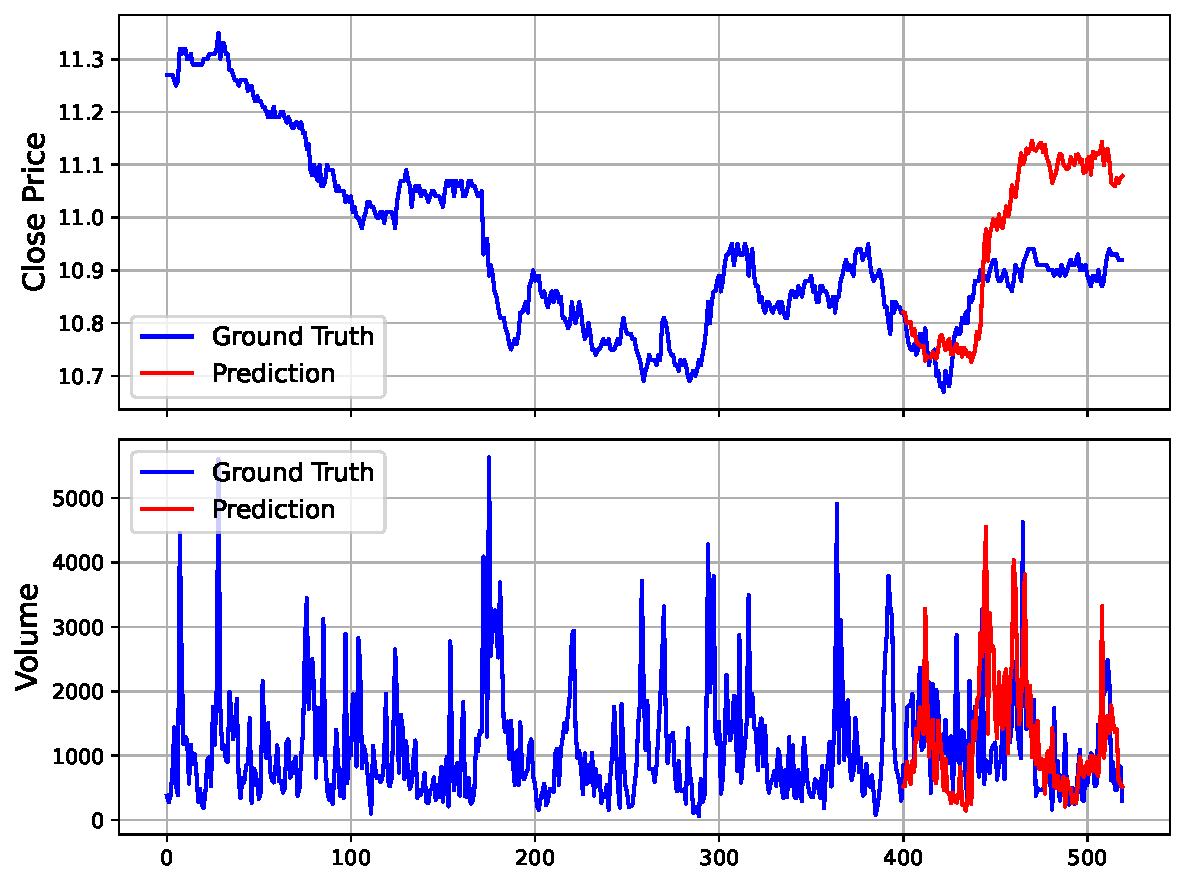
\includegraphics[width=\linewidth]{pred_imgs/pred_visualize_stock_XSHG_600977_5min_Kronos_small.pdf}
        \caption{$\text{Kronos}_{small}$}
    \end{subfigure}
    \hfill
    \begin{subfigure}[b]{0.33\textwidth}
        \centering
        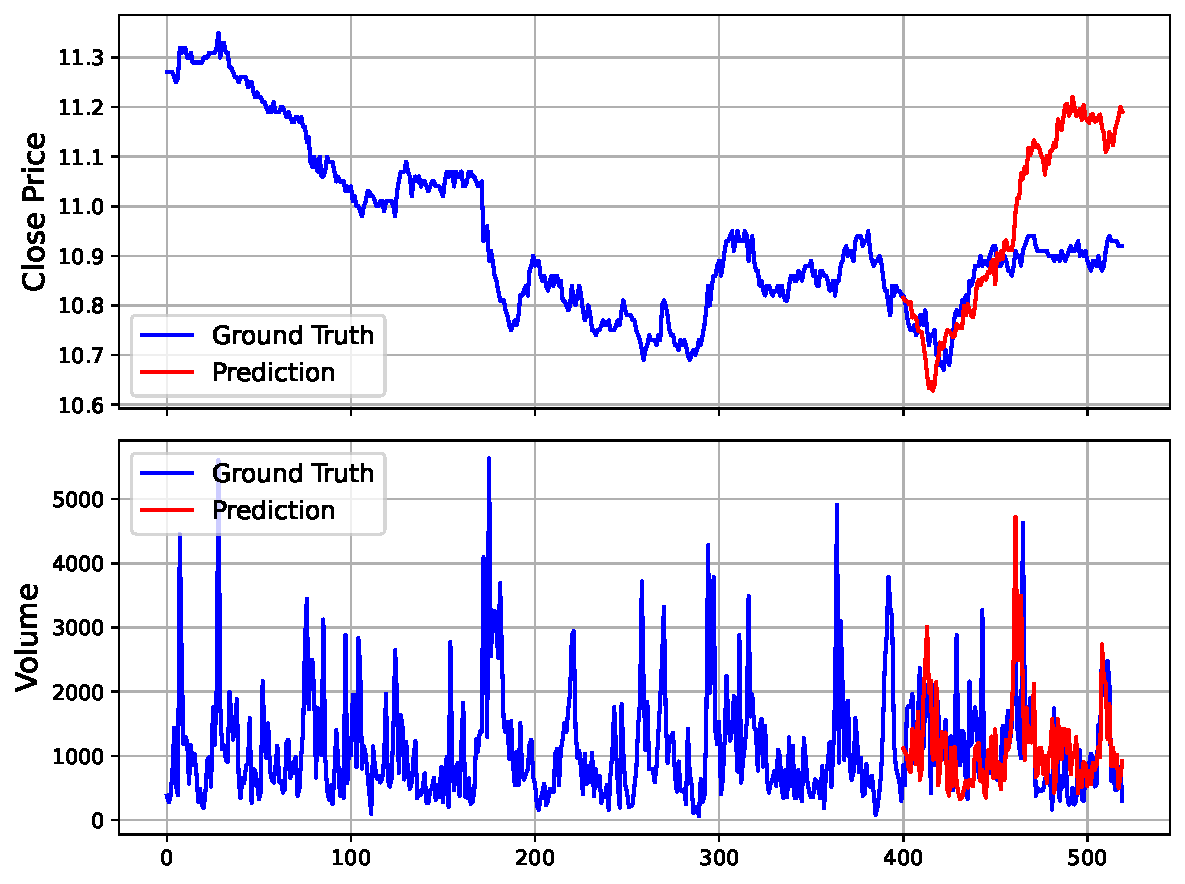
\includegraphics[width=\linewidth]{pred_imgs/pred_visualize_stock_XSHG_600977_5min_Kronos_base.pdf}
        \caption{$\text{Kronos}_{base}$}
    \end{subfigure}
    \hfill
    \begin{subfigure}[b]{0.33\textwidth}
        \centering
        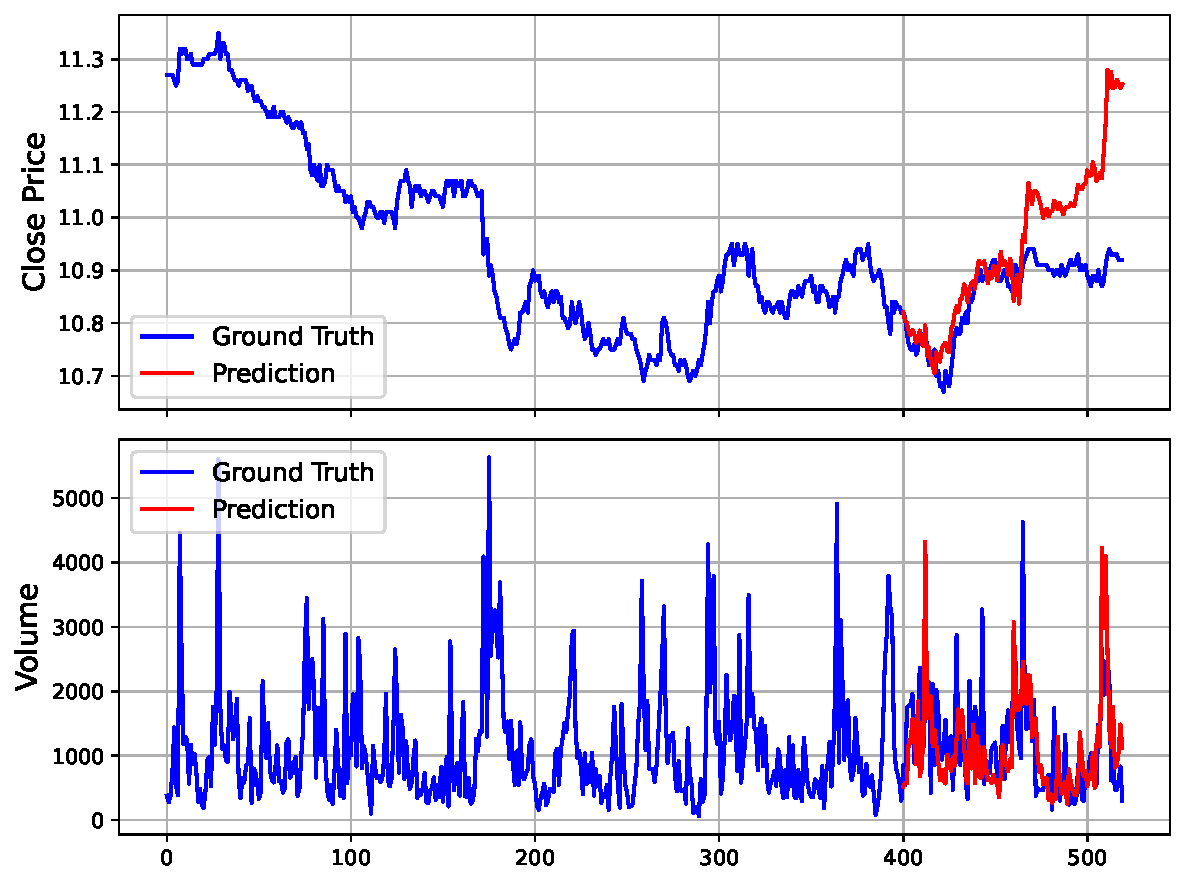
\includegraphics[width=\linewidth]{pred_imgs/pred_visualize_stock_XSHG_600977_5min_Kronos_large.pdf}
        \caption{$\text{Kronos}_{large}$}
    \end{subfigure}

    \vspace{0.1cm}

    \begin{subfigure}[b]{0.33\textwidth}
        \centering
        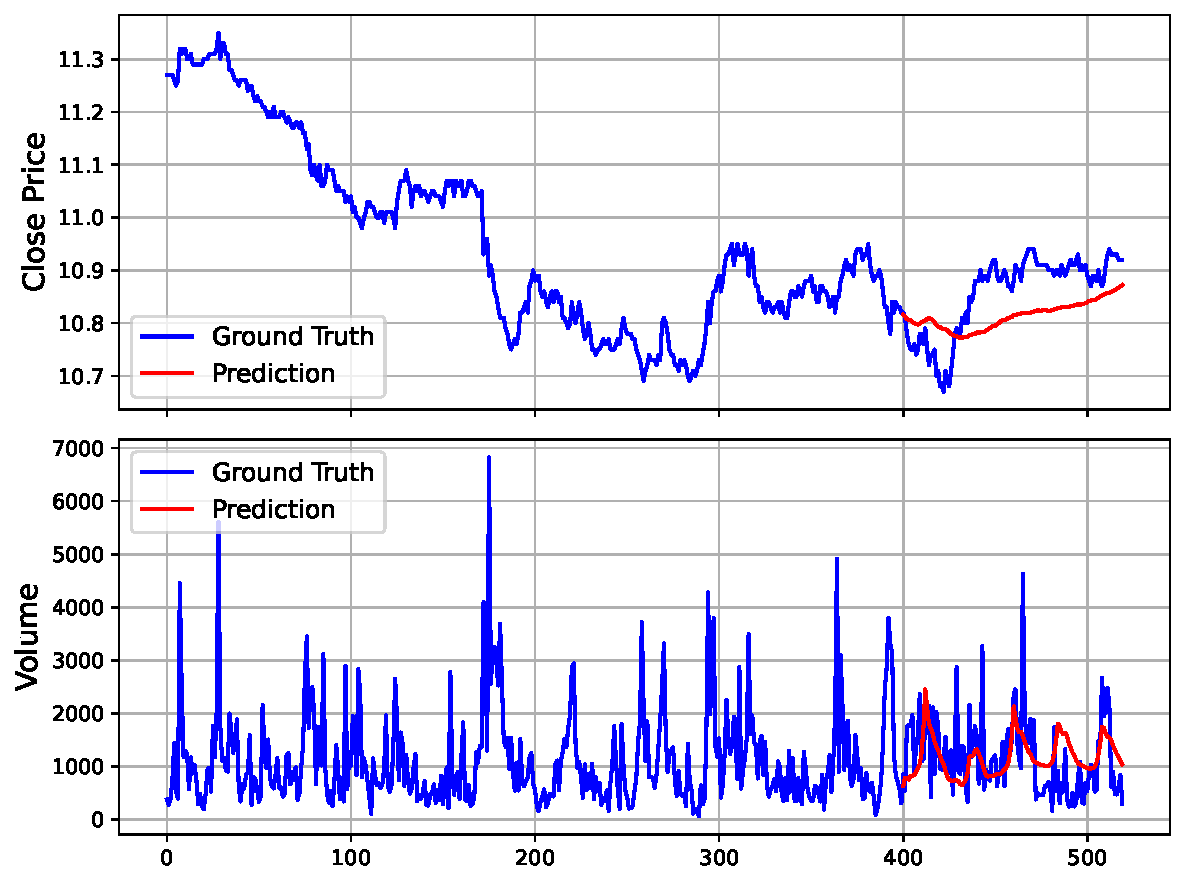
\includegraphics[width=\linewidth]{pred_imgs/pred_visualize_stock_XSHG_600977_5min_TimeMOE_small.pdf}
        \caption{$\text{TimeMOE}_{small}$}
    \end{subfigure}
    \hfill
    \begin{subfigure}[b]{0.33\textwidth}
        \centering
        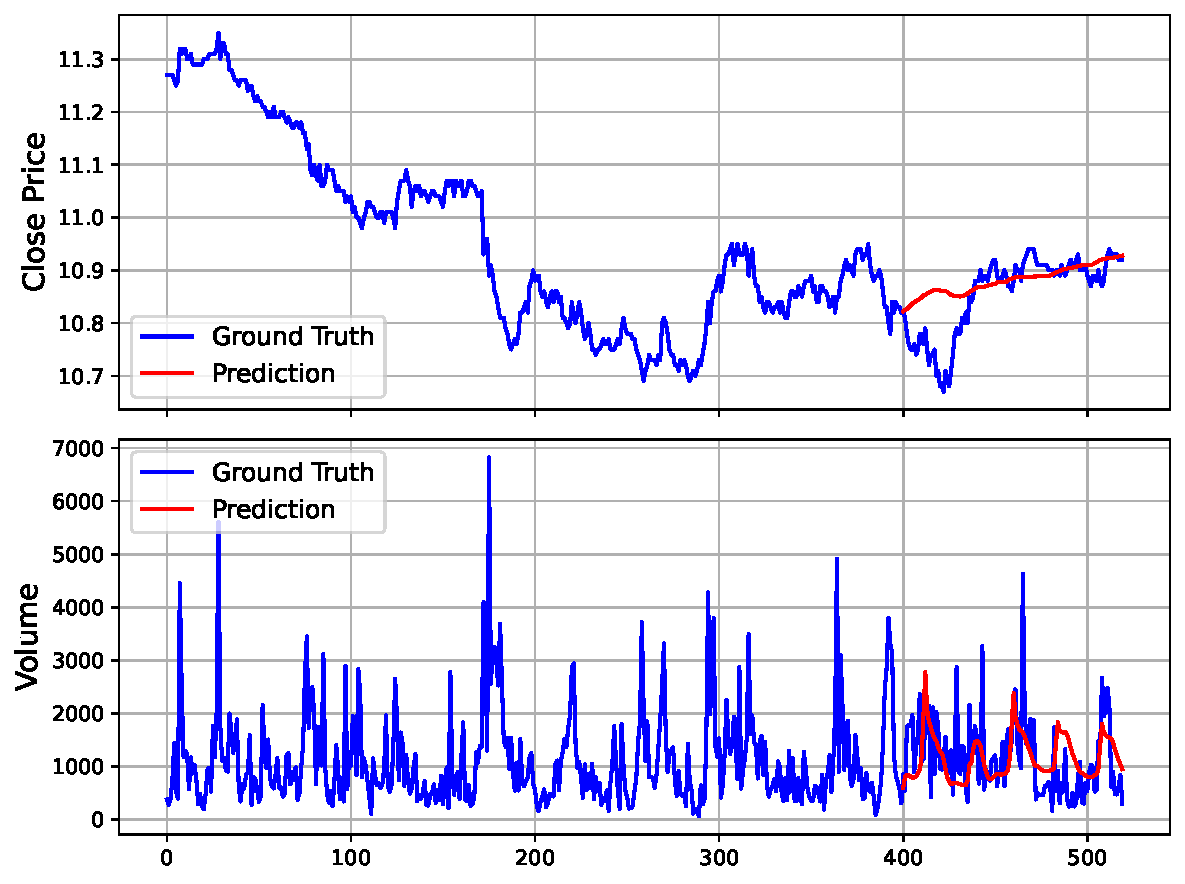
\includegraphics[width=\linewidth]{pred_imgs/pred_visualize_stock_XSHG_600977_5min_TimeMOE_large.pdf}
        \caption{$\text{TimeMOE}_{large}$}
    \end{subfigure}
    \hfill
    \begin{subfigure}[b]{0.33\textwidth}
        \centering
        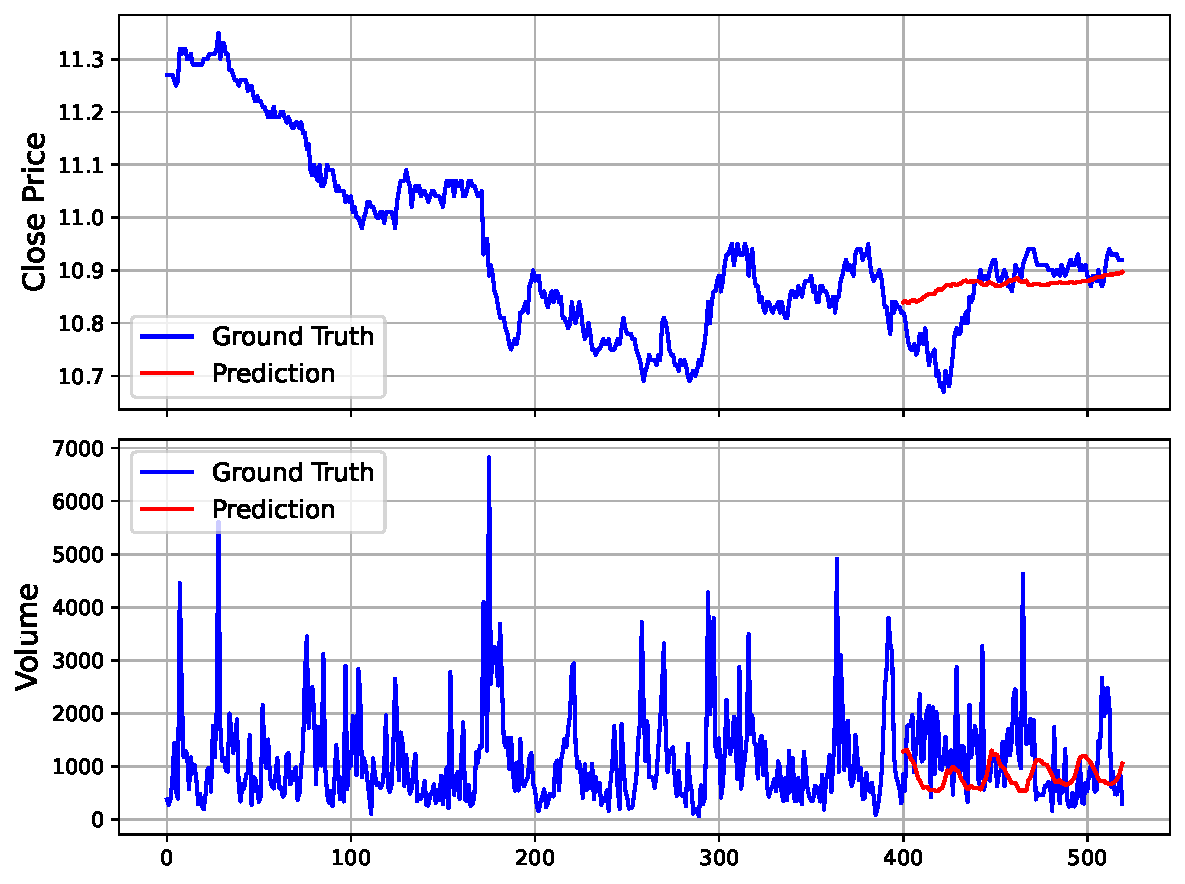
\includegraphics[width=\linewidth]{pred_imgs/pred_visualize_stock_XSHG_600977_5min_TimesFM.pdf}
        \caption{TimesFM}
    \end{subfigure}

    \vspace{0.1cm}

    \begin{subfigure}[b]{0.33\textwidth}
        \centering
        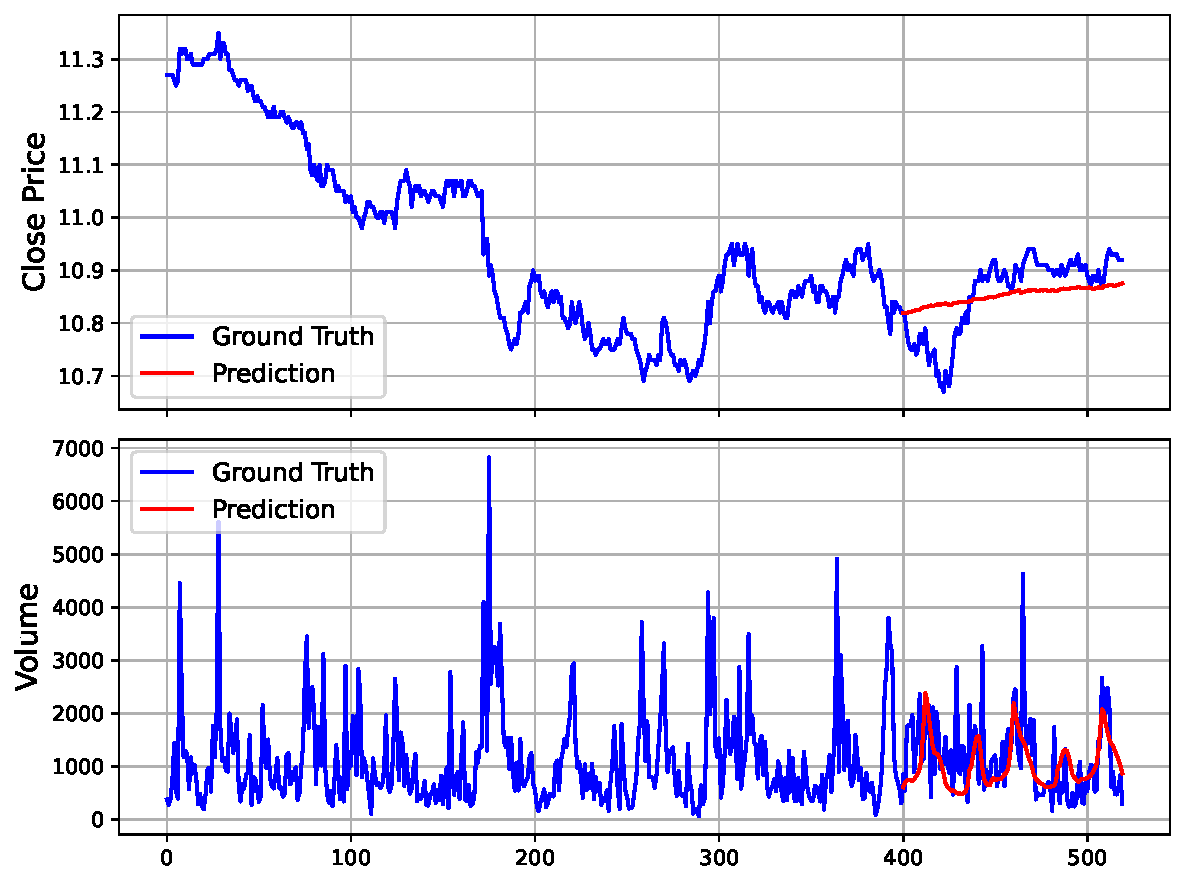
\includegraphics[width=\linewidth]{pred_imgs/pred_visualize_stock_XSHG_600977_5min_Chronos_small.pdf}
        \caption{$\text{Chronos}_{small}$}
    \end{subfigure}
    \hfill
    \begin{subfigure}[b]{0.33\textwidth}
        \centering
        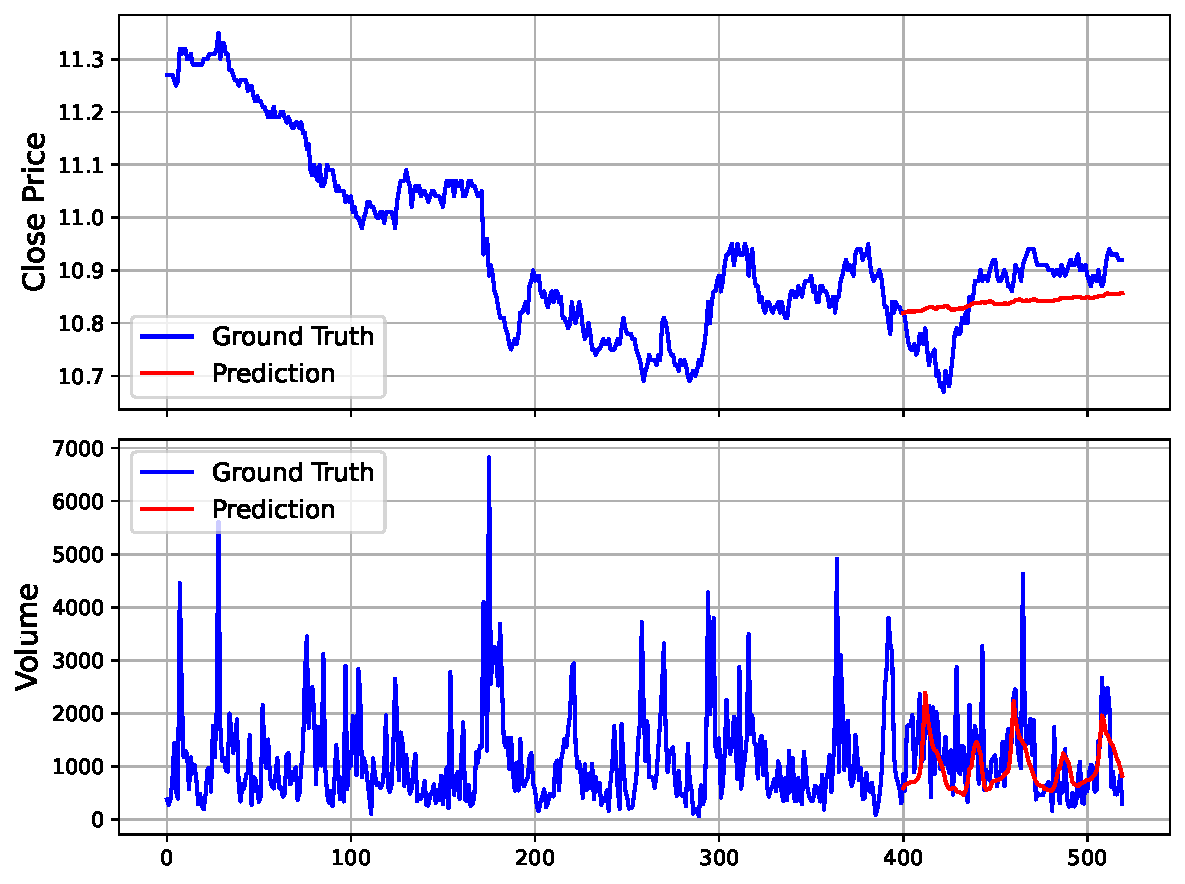
\includegraphics[width=\linewidth]{pred_imgs/pred_visualize_stock_XSHG_600977_5min_Chronos_base.pdf}
        \caption{$\text{Chronos}_{base}$}
    \end{subfigure}
    \hfill
    \begin{subfigure}[b]{0.33\textwidth}
        \centering
        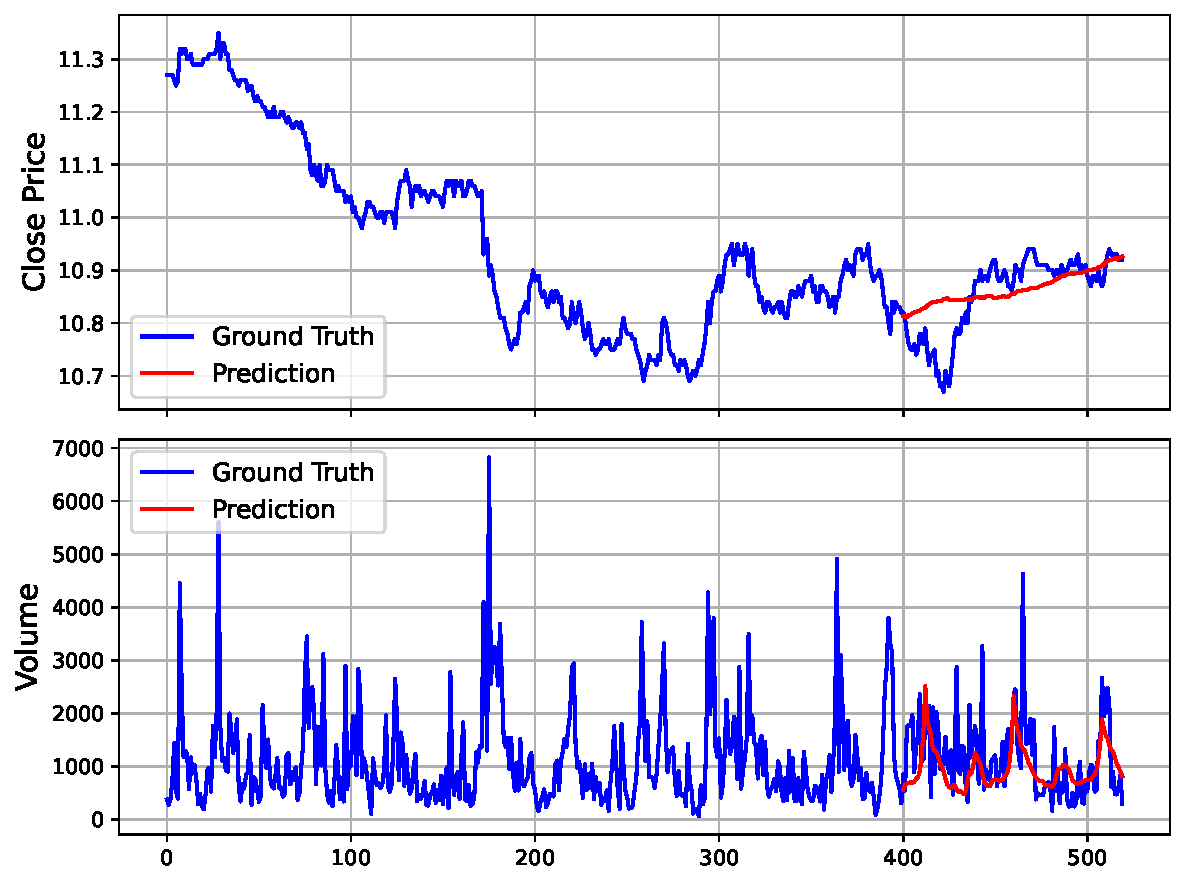
\includegraphics[width=\linewidth]{pred_imgs/pred_visualize_stock_XSHG_600977_5min_Chronos_large.pdf}
        \caption{$\text{Chronos}_{large}$}
    \end{subfigure}

    \vspace{0.1cm}

    \begin{subfigure}[b]{0.33\textwidth}
        \centering
        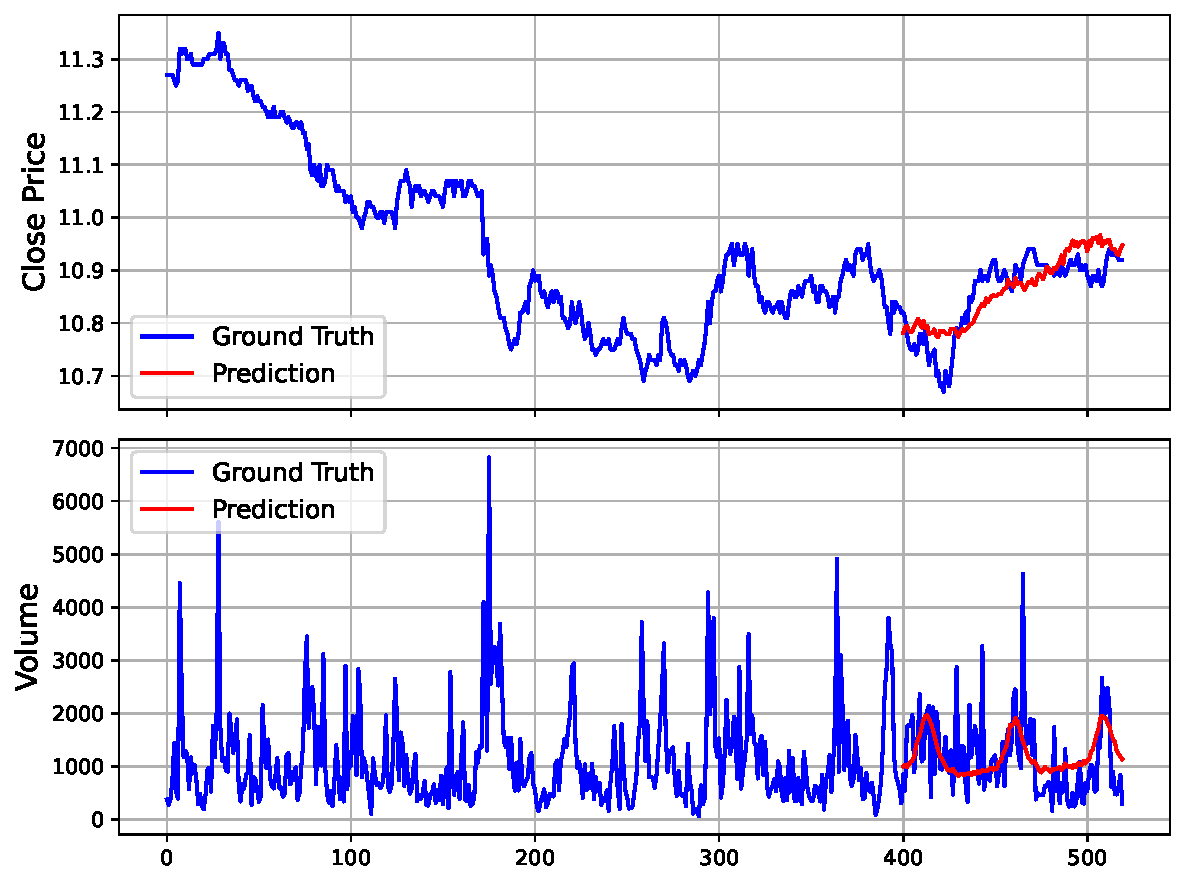
\includegraphics[width=\linewidth]{pred_imgs/pred_visualize_stock_XSHG_600977_5min_iTransformer.pdf}
        \caption{iTransformer}
    \end{subfigure}
    \hfill
    \begin{subfigure}[b]{0.33\textwidth}
        \centering
        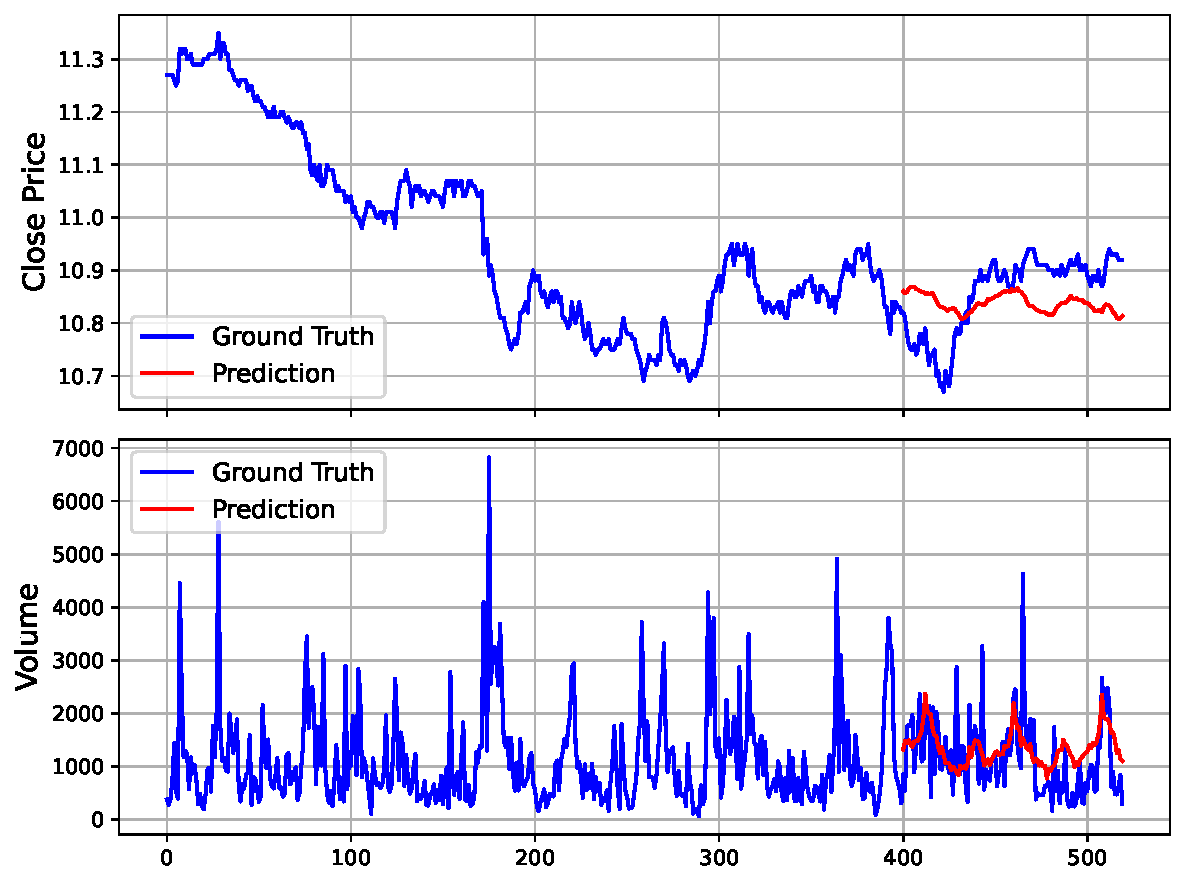
\includegraphics[width=\linewidth]{pred_imgs/pred_visualize_stock_XSHG_600977_5min_DLinear.pdf}
        \caption{DLinear}
    \end{subfigure}
    \hfill
    \begin{subfigure}[b]{0.33\textwidth}
        \centering
        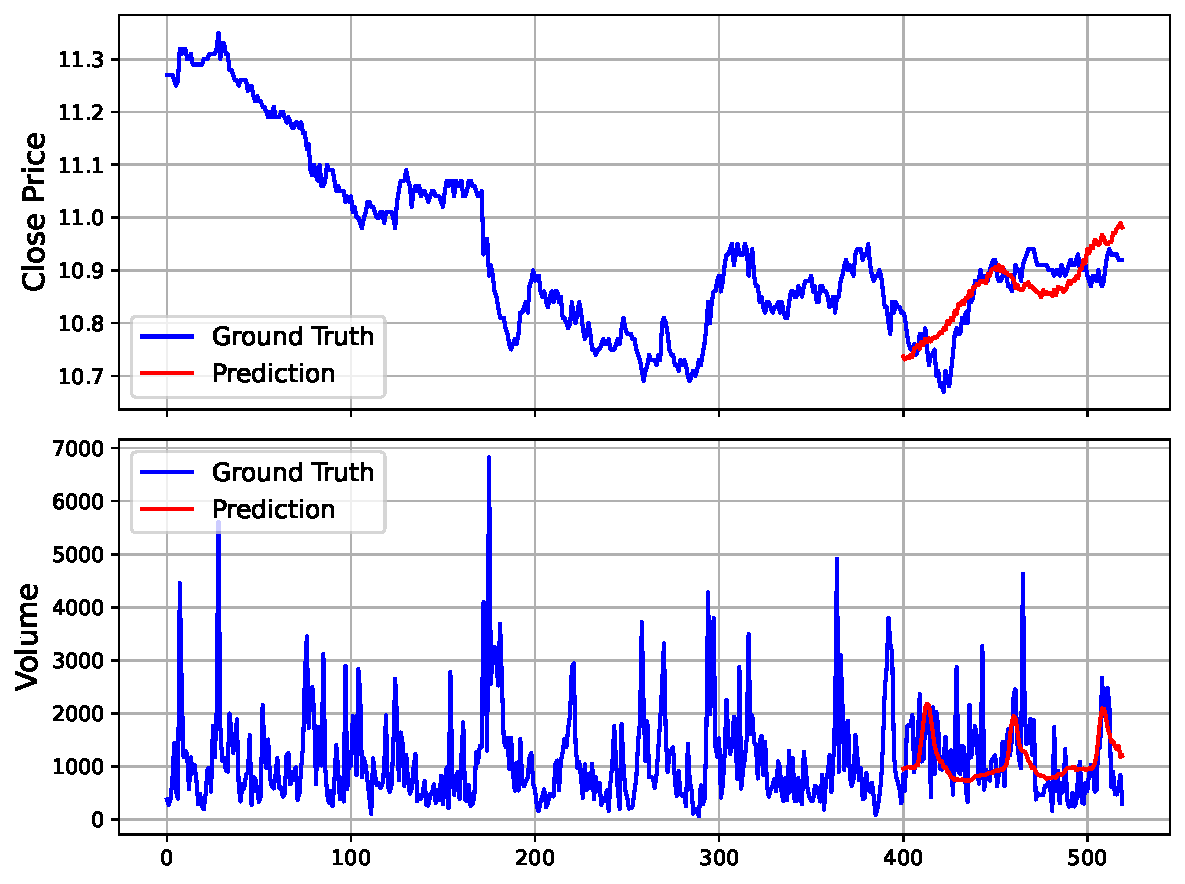
\includegraphics[width=\linewidth]{pred_imgs/pred_visualize_stock_XSHG_600977_5min_TimesNet.pdf}
        \caption{TimesNet}
    \end{subfigure}

    \caption{5분 K-line 데이터를 기반으로 한 China Film Co.,Ltd. (SSE: 600977)의 `Close Price'와 `Volume' 예측 결과. 모델은 400스텝 look-back 윈도우를 사용하여 120스텝 horizon을 예측한다. \textcolor{blue}{Blue} 선은 정답값을 나타내고 \textcolor{red}{red} 선은 모델의 예측값을 나타낸다.}
    \label{fig:pred_case_1}
\end{figure*}

\begin{figure*}[ht]
    \centering

    \begin{subfigure}[b]{0.33\textwidth}
        \centering
        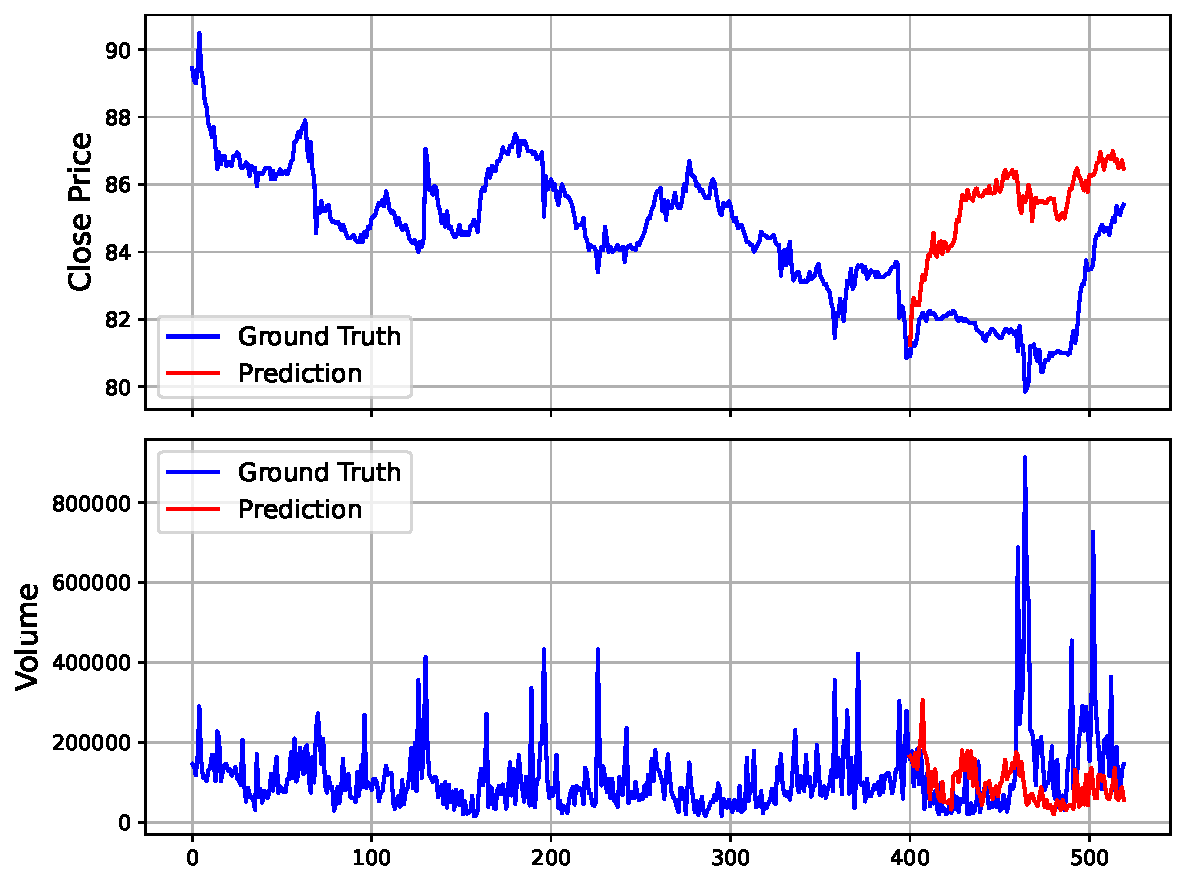
\includegraphics[width=\linewidth]{pred_imgs/pred_visualize_stock_XHKG_9992_5min_Kronos_small.pdf}
        \caption{$\text{Kronos}_{small}$}
    \end{subfigure}
    \hfill
    \begin{subfigure}[b]{0.33\textwidth}
        \centering
        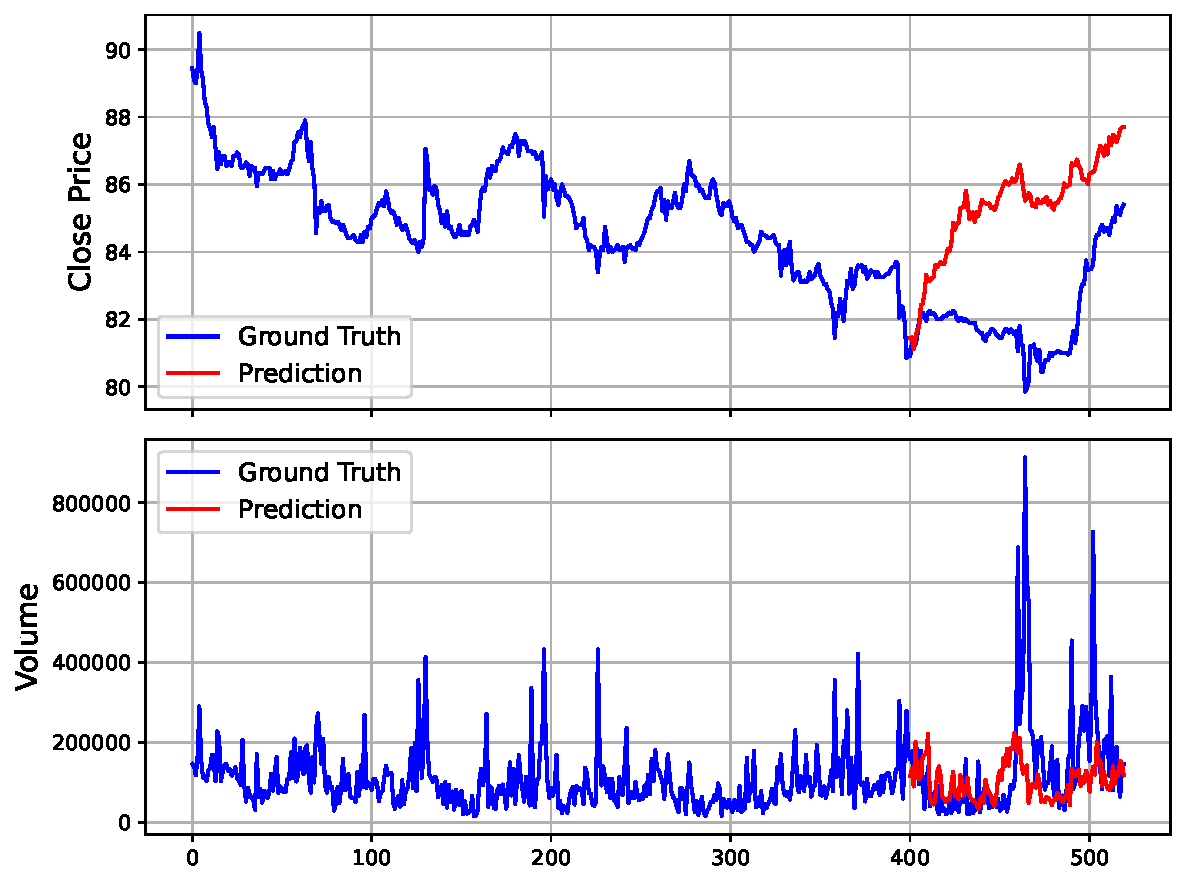
\includegraphics[width=\linewidth]{pred_imgs/pred_visualize_stock_XHKG_9992_5min_Kronos_base.pdf}
        \caption{$\text{Kronos}_{base}$}
    \end{subfigure}
    \hfill
    \begin{subfigure}[b]{0.33\textwidth}
        \centering
        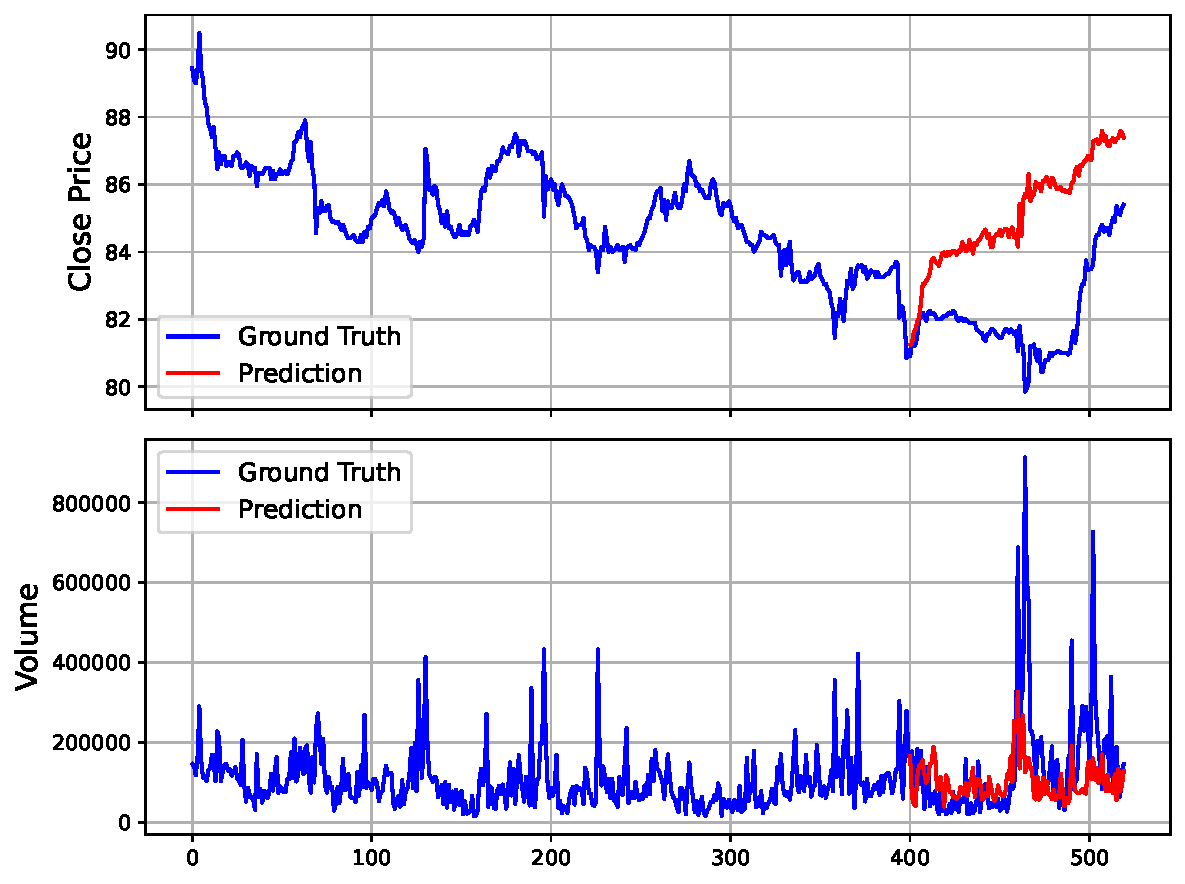
\includegraphics[width=\linewidth]{pred_imgs/pred_visualize_stock_XHKG_9992_5min_Kronos_large.pdf}
        \caption{$\text{Kronos}_{large}$}
    \end{subfigure}

    \vspace{0.1cm}

    \begin{subfigure}[b]{0.33\textwidth}
        \centering
        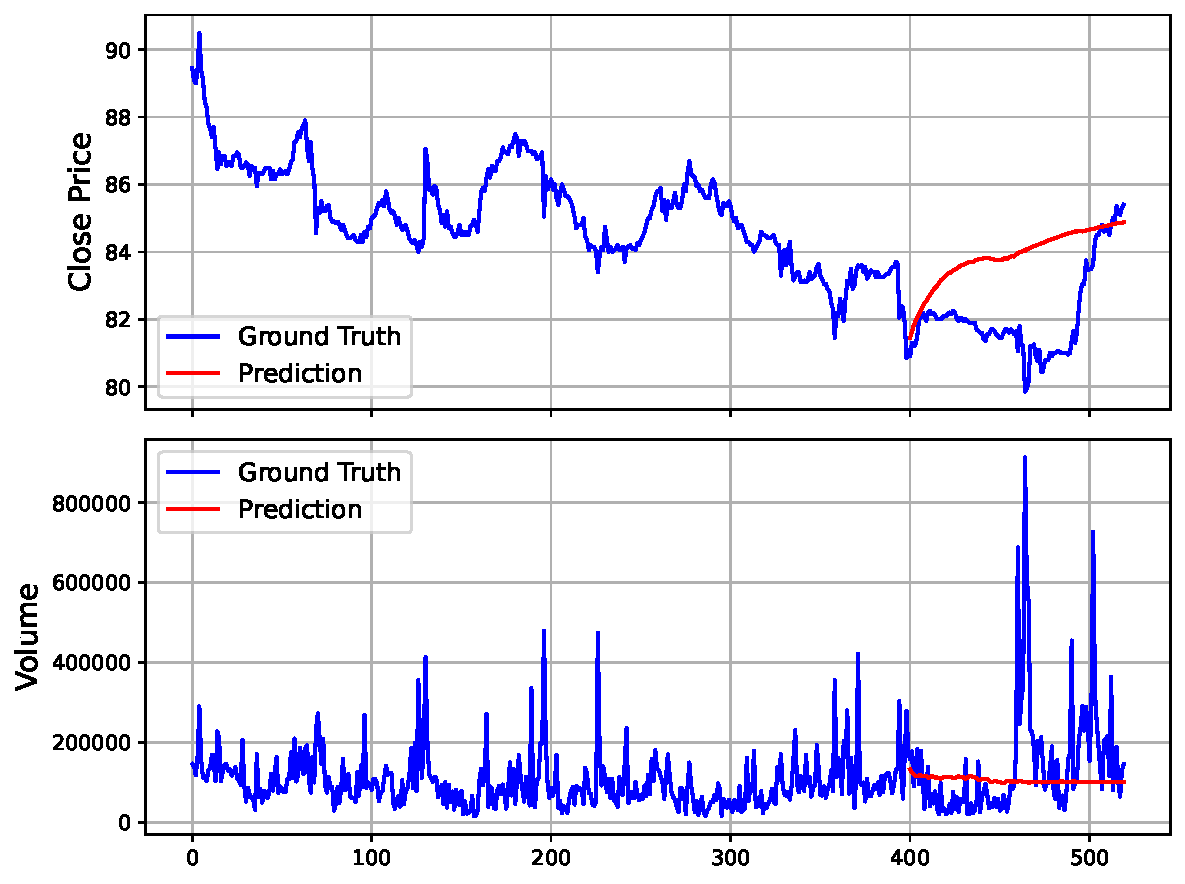
\includegraphics[width=\linewidth]{pred_imgs/pred_visualize_stock_XHKG_9992_5min_TimeMOE_small.pdf}
        \caption{$\text{TimeMOE}_{small}$}
    \end{subfigure}
    \hfill
    \begin{subfigure}[b]{0.33\textwidth}
        \centering
        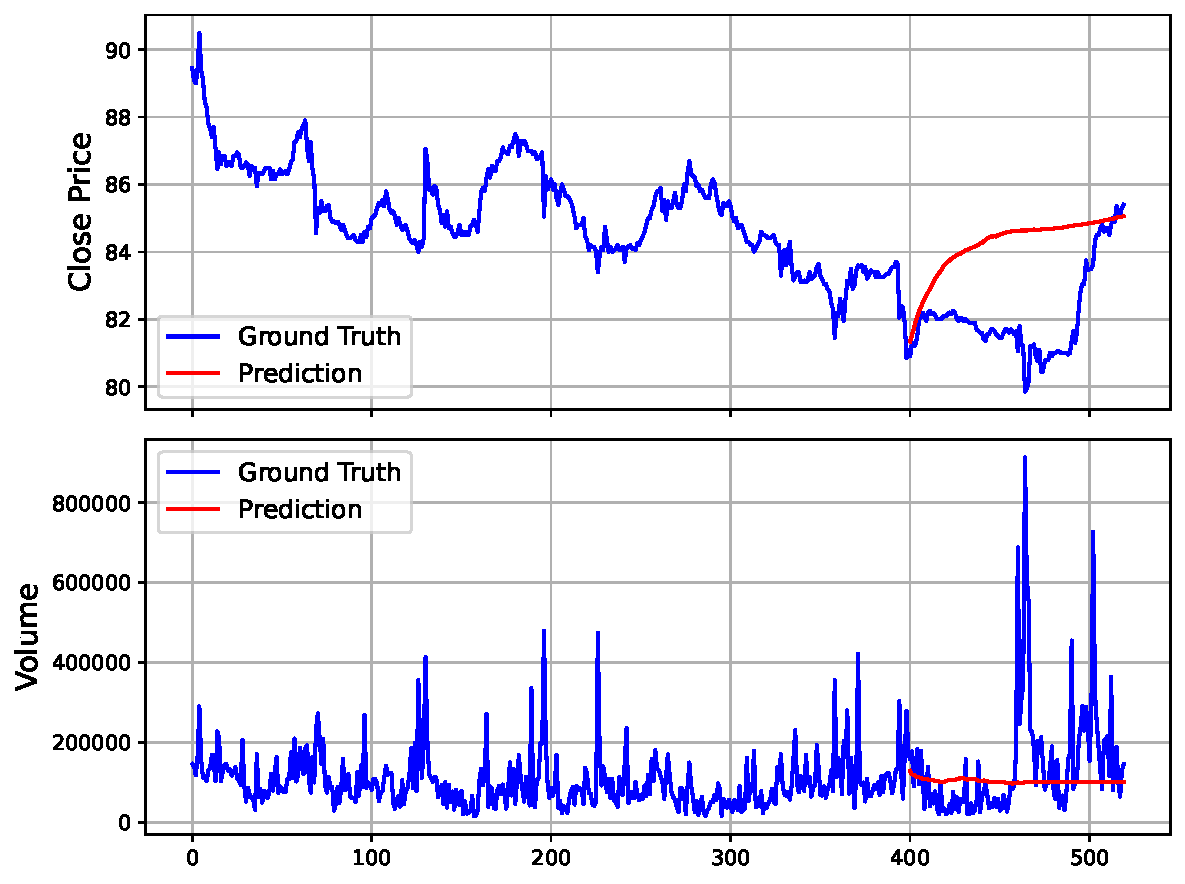
\includegraphics[width=\linewidth]{pred_imgs/pred_visualize_stock_XHKG_9992_5min_TimeMOE_large.pdf}
        \caption{$\text{TimeMOE}_{large}$}
    \end{subfigure}
    \hfill
    \begin{subfigure}[b]{0.33\textwidth}
        \centering
        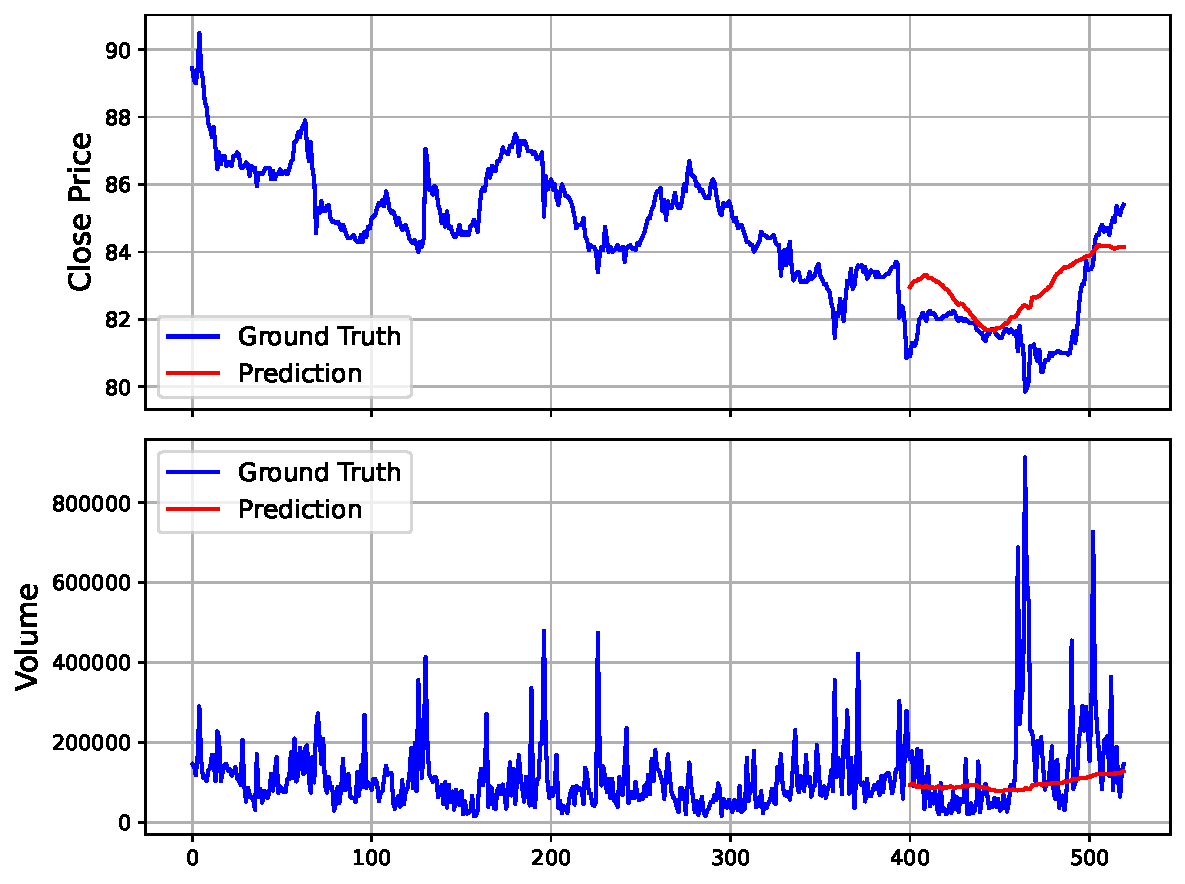
\includegraphics[width=\linewidth]{pred_imgs/pred_visualize_stock_XHKG_9992_5min_TimesFM.pdf}
        \caption{TimesFM}
    \end{subfigure}

    \vspace{0.1cm}

    \begin{subfigure}[b]{0.33\textwidth}
        \centering
        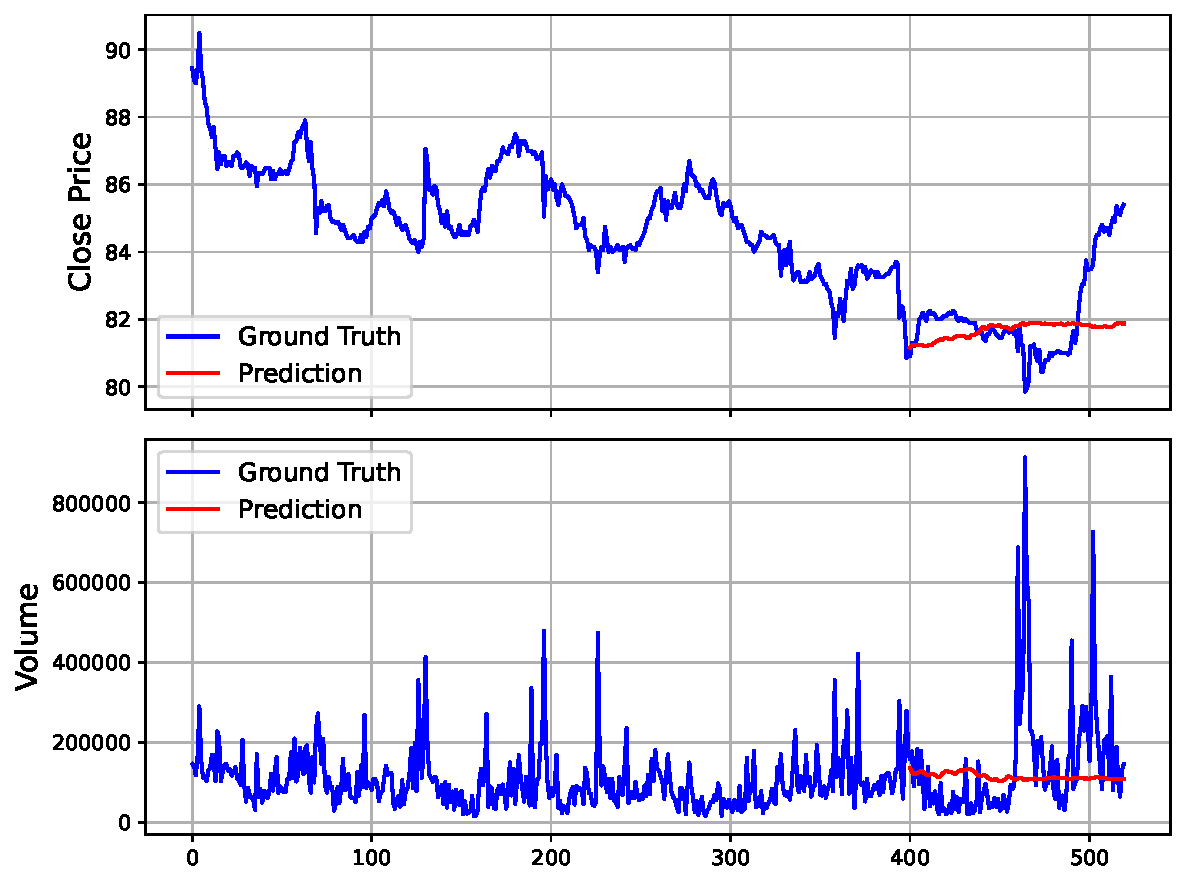
\includegraphics[width=\linewidth]{pred_imgs/pred_visualize_stock_XHKG_9992_5min_Chronos_small.pdf}
        \caption{$\text{Chronos}_{small}$}
    \end{subfigure}
    \hfill
    \begin{subfigure}[b]{0.33\textwidth}
        \centering
        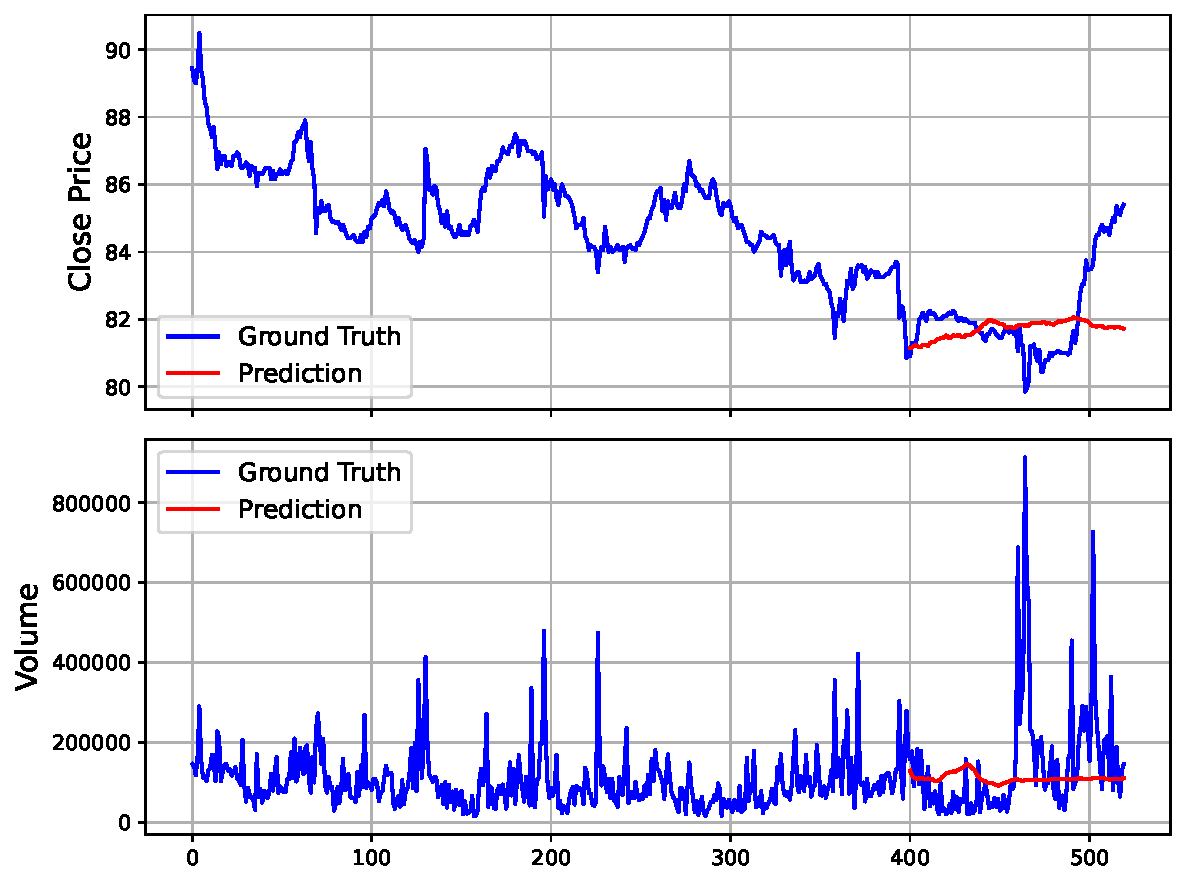
\includegraphics[width=\linewidth]{pred_imgs/pred_visualize_stock_XHKG_9992_5min_Chronos_base.pdf}
        \caption{$\text{Chronos}_{base}$}
    \end{subfigure}
    \hfill
    \begin{subfigure}[b]{0.33\textwidth}
        \centering
        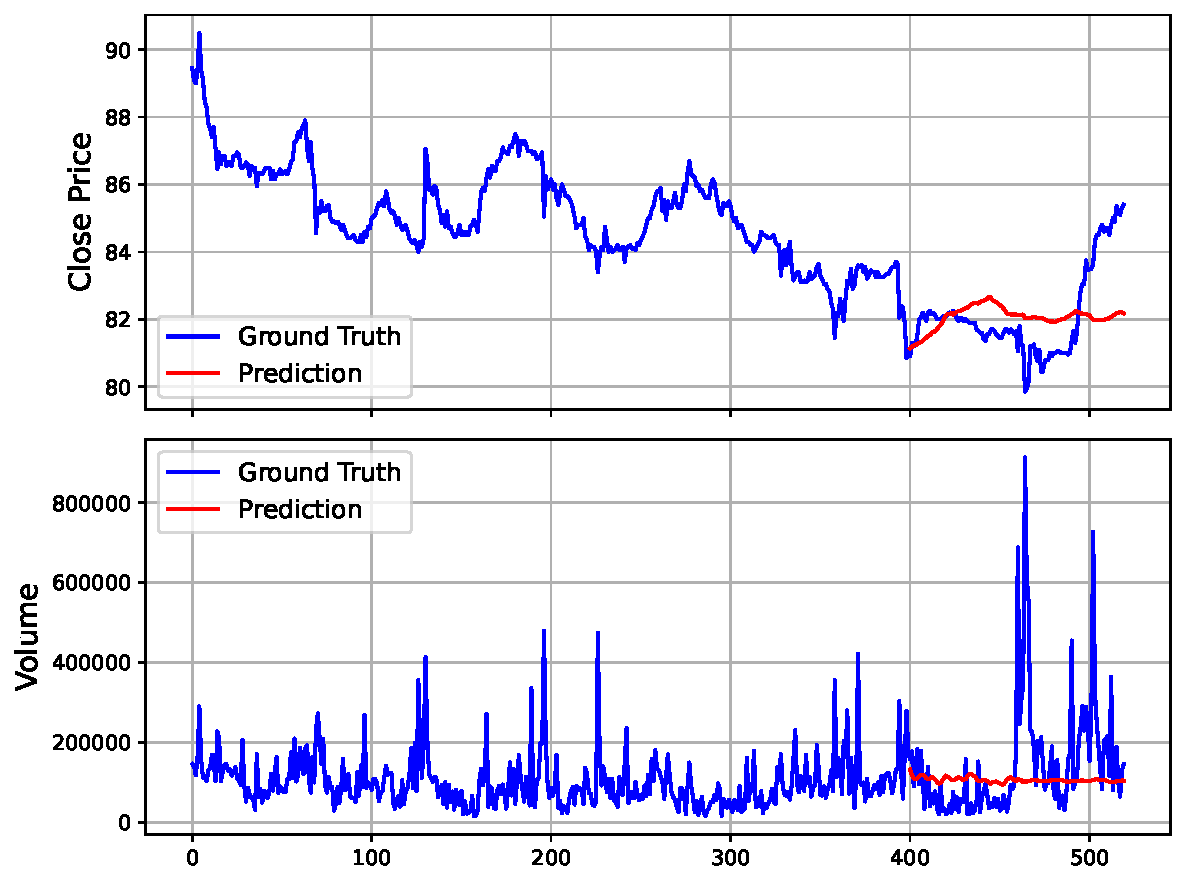
\includegraphics[width=\linewidth]{pred_imgs/pred_visualize_stock_XHKG_9992_5min_Chronos_large.pdf}
        \caption{$\text{Chronos}_{large}$}
    \end{subfigure}

    \vspace{0.1cm}

    \begin{subfigure}[b]{0.33\textwidth}
        \centering
        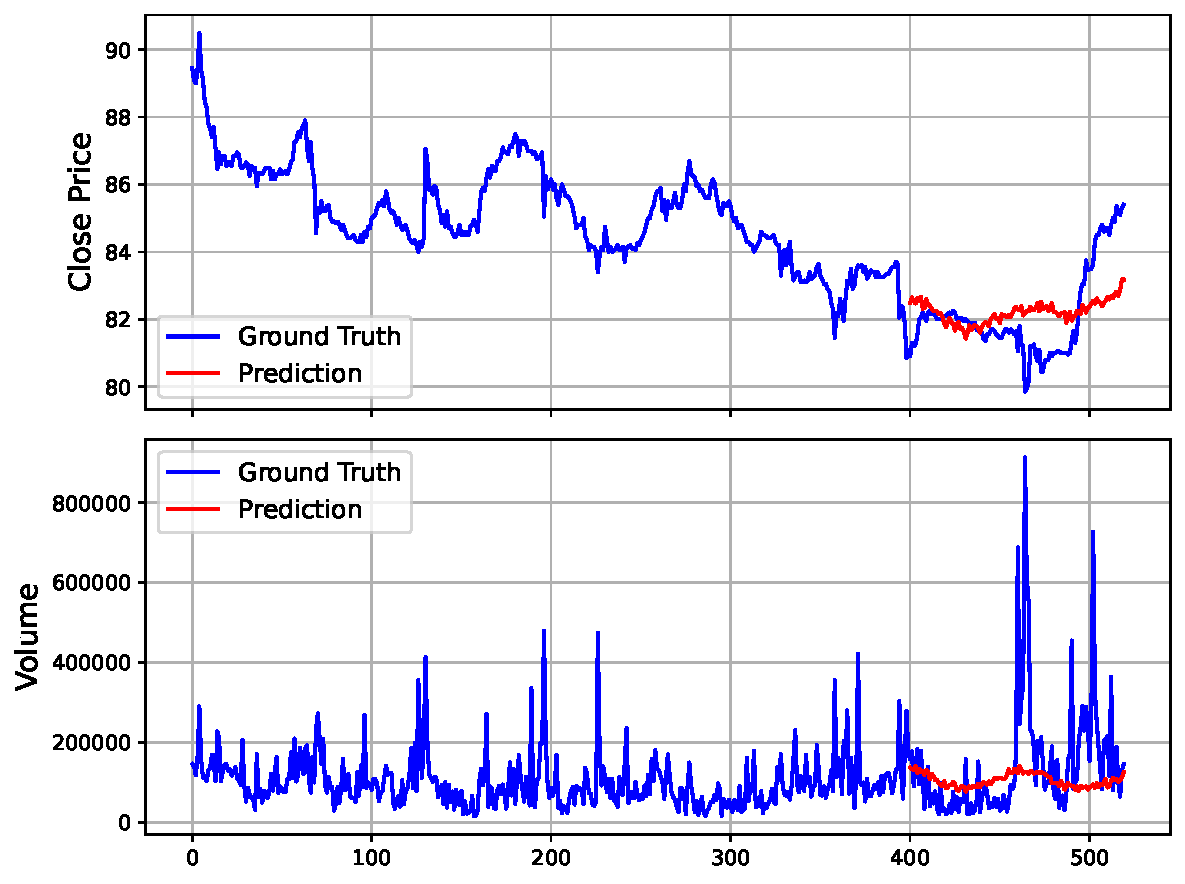
\includegraphics[width=\linewidth]{pred_imgs/pred_visualize_stock_XHKG_9992_5min_iTransformer.pdf}
        \caption{iTransformer}
    \end{subfigure}
    \hfill
    \begin{subfigure}[b]{0.33\textwidth}
        \centering
        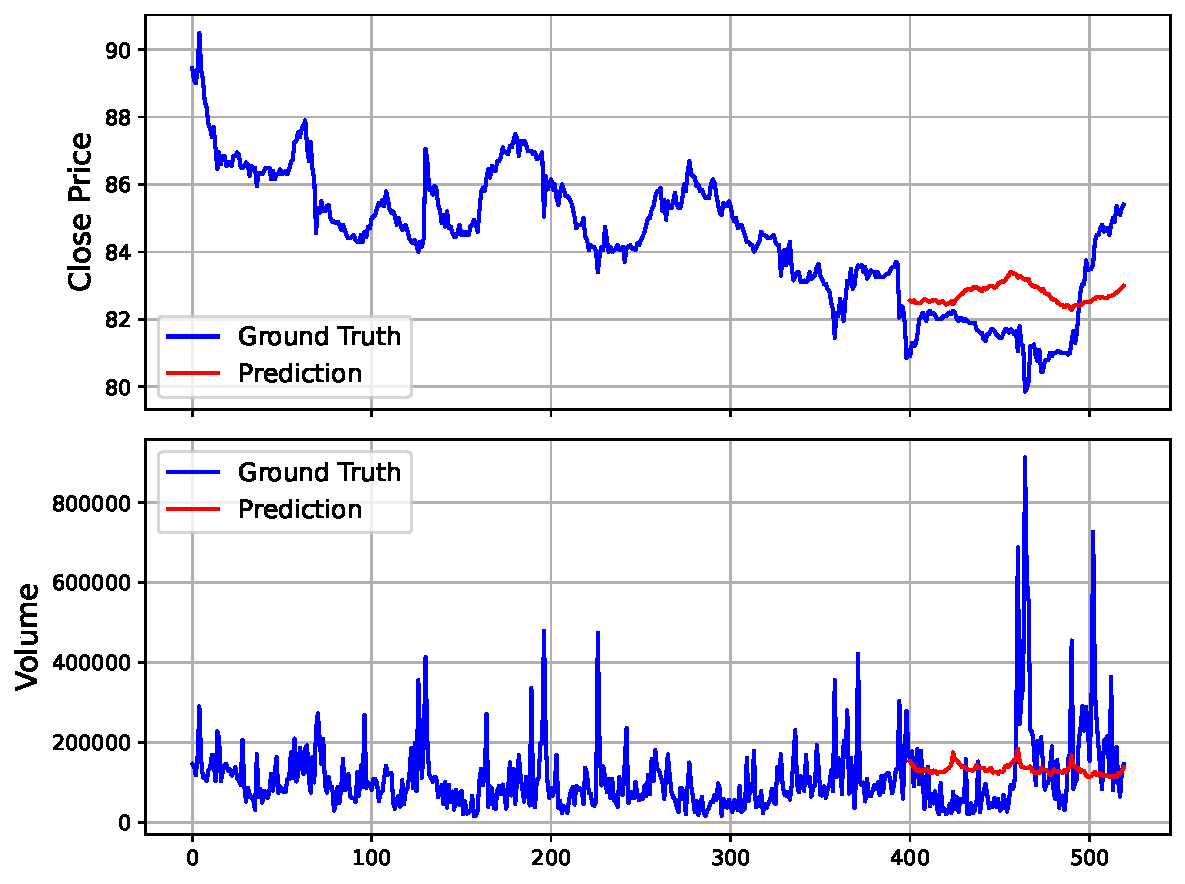
\includegraphics[width=\linewidth]{pred_imgs/pred_visualize_stock_XHKG_9992_5min_DLinear.pdf}
        \caption{DLinear}
    \end{subfigure}
    \hfill
    \begin{subfigure}[b]{0.33\textwidth}
        \centering
        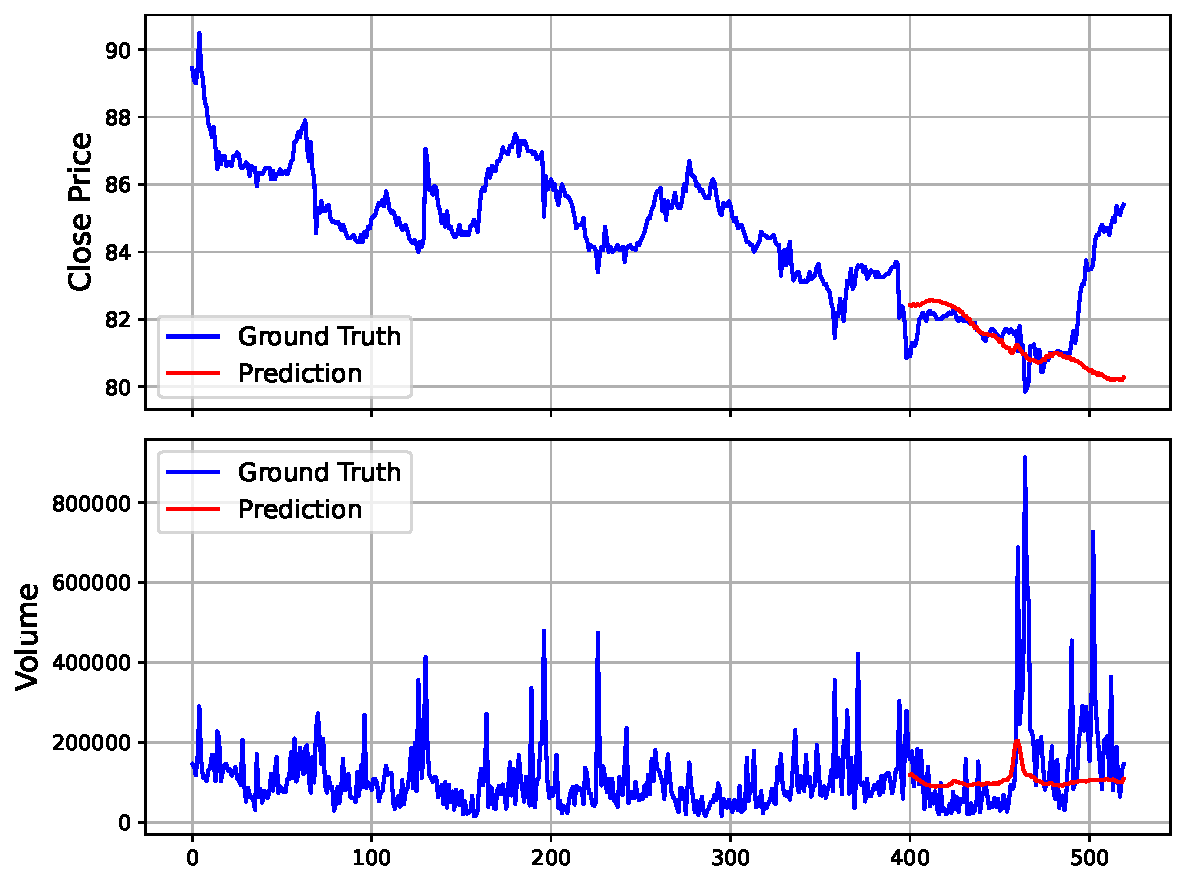
\includegraphics[width=\linewidth]{pred_imgs/pred_visualize_stock_XHKG_9992_5min_TimesNet.pdf}
        \caption{TimesNet}
    \end{subfigure}

    \caption{5분 K-line 데이터를 기반으로 한 Pop Mart (HKEX: 09992)의 `Close Price'와 `Volume' 예측 결과. 모델은 400스텝 look-back 윈도우를 사용하여 120스텝 horizon을 예측한다. \textcolor{blue}{Blue} 선은 정답값을 나타내고 \textcolor{red}{red} 선은 모델의 예측값을 나타낸다.}
    \label{fig:pred_case_2}
\end{figure*}


\begin{figure*}[ht]
    \centering

    \begin{subfigure}[b]{0.33\textwidth}
        \centering
        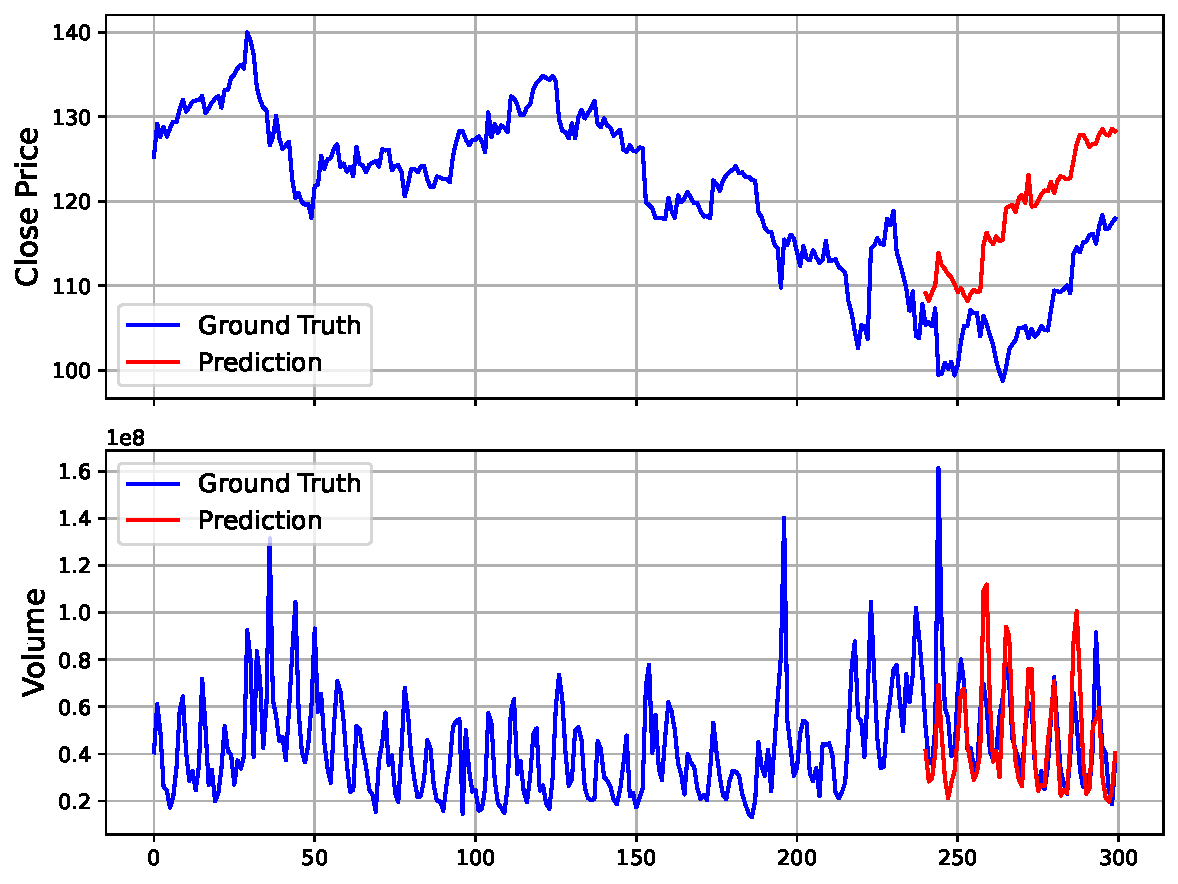
\includegraphics[width=\linewidth]{pred_imgs/pred_visualize_stock_XNAS_NVDA_60min_Kronos_small.pdf}
        \caption{$\text{Kronos}_{small}$}
    \end{subfigure}
    \hfill
    \begin{subfigure}[b]{0.33\textwidth}
        \centering
        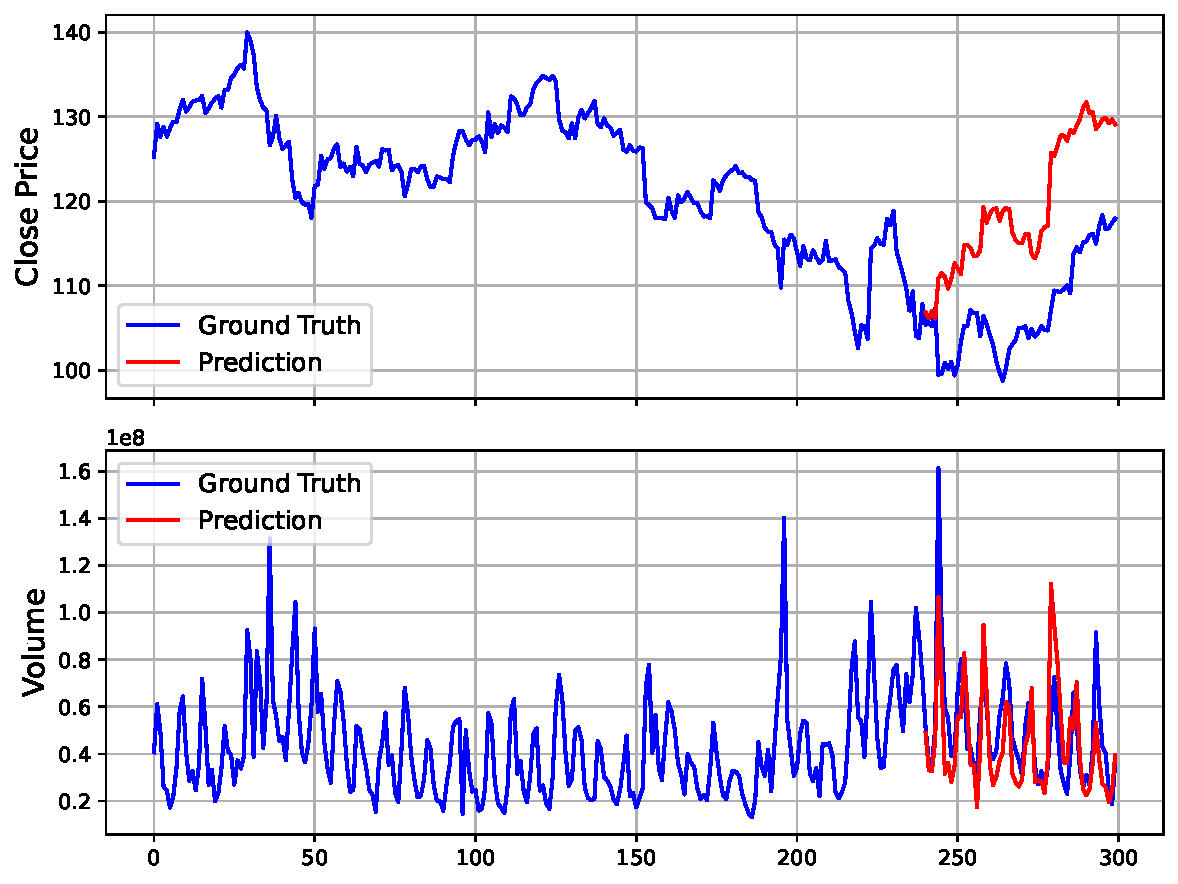
\includegraphics[width=\linewidth]{pred_imgs/pred_visualize_stock_XNAS_NVDA_60min_Kronos_base.pdf}
        \caption{$\text{Kronos}_{base}$}
    \end{subfigure}
    \hfill
    \begin{subfigure}[b]{0.33\textwidth}
        \centering
        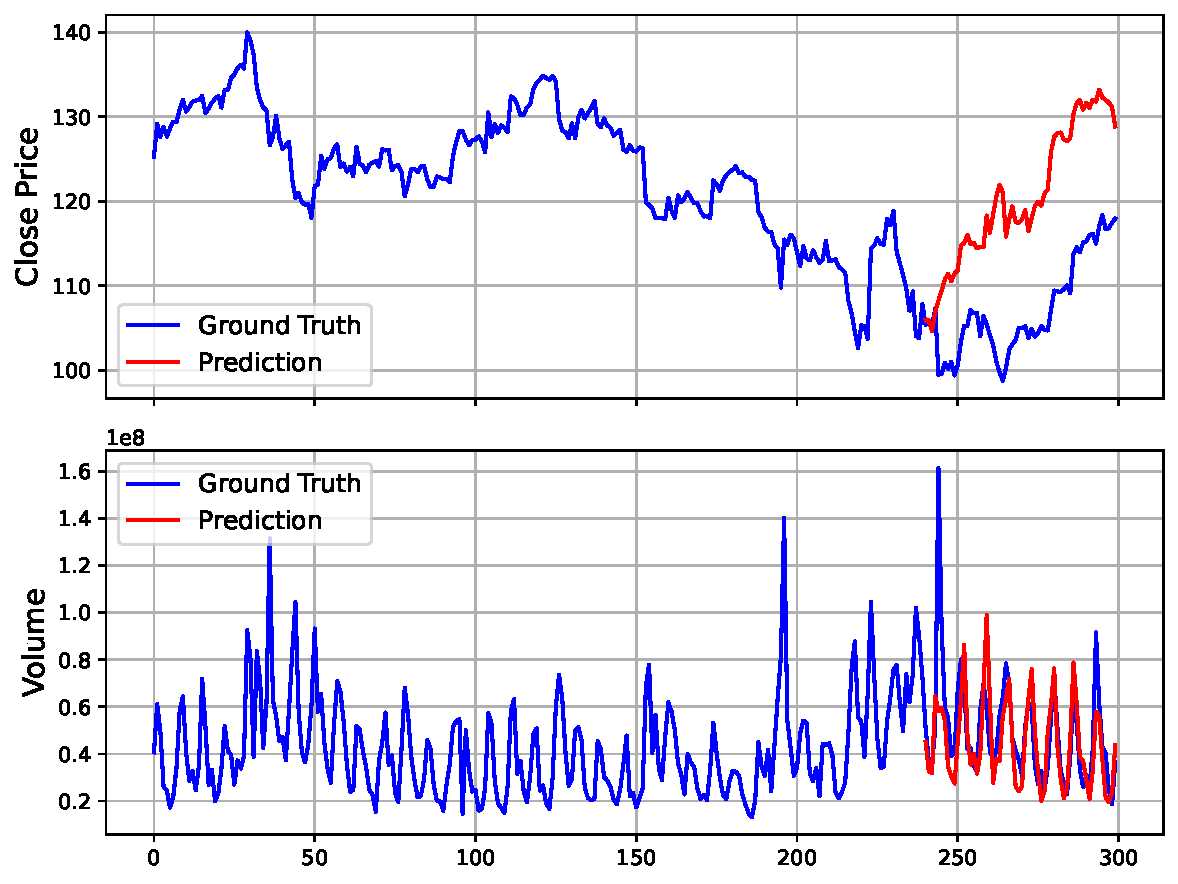
\includegraphics[width=\linewidth]{pred_imgs/pred_visualize_stock_XNAS_NVDA_60min_Kronos_large.pdf}
        \caption{$\text{Kronos}_{large}$}
    \end{subfigure}

    \vspace{0.1cm}

    \begin{subfigure}[b]{0.33\textwidth}
        \centering
        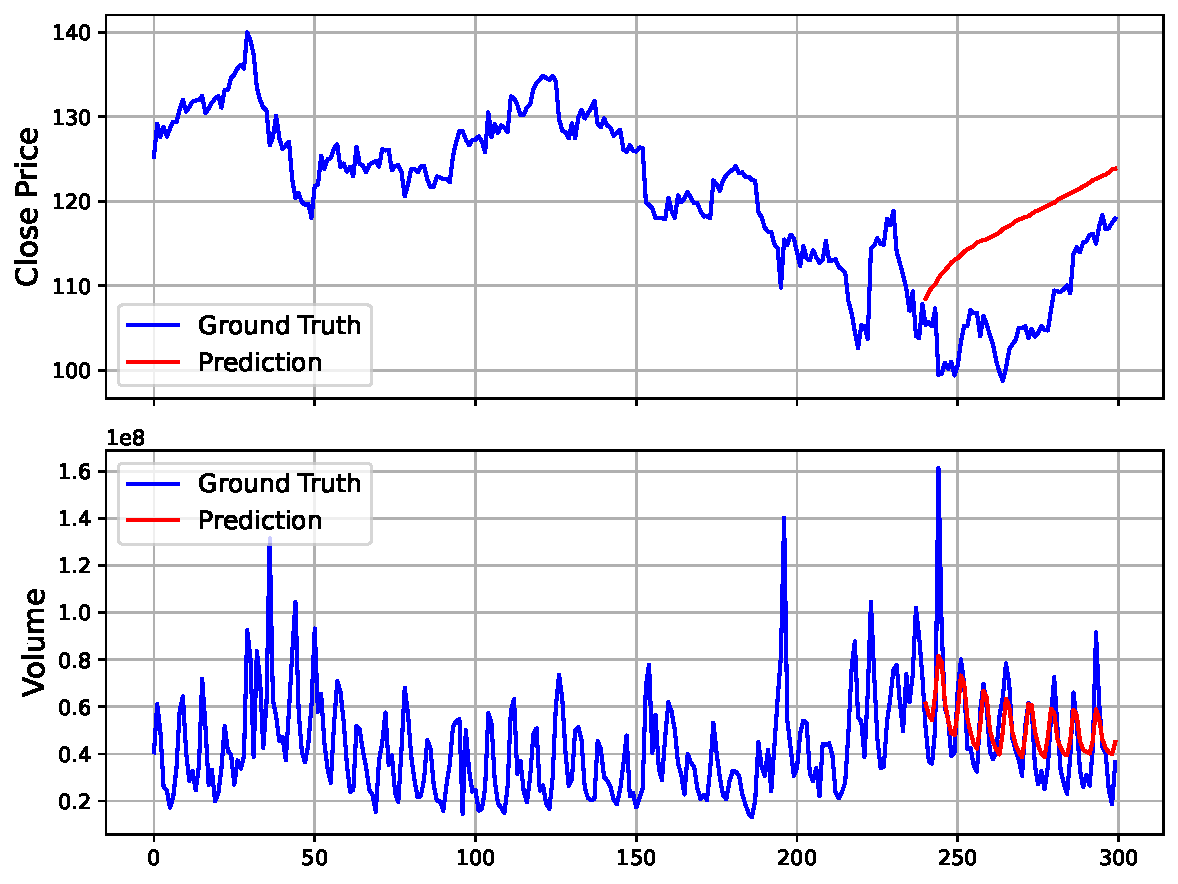
\includegraphics[width=\linewidth]{pred_imgs/pred_visualize_stock_XNAS_NVDA_60min_TimeMOE_small.pdf}
        \caption{$\text{TimeMOE}_{small}$}
    \end{subfigure}
    \hfill
    \begin{subfigure}[b]{0.33\textwidth}
        \centering
        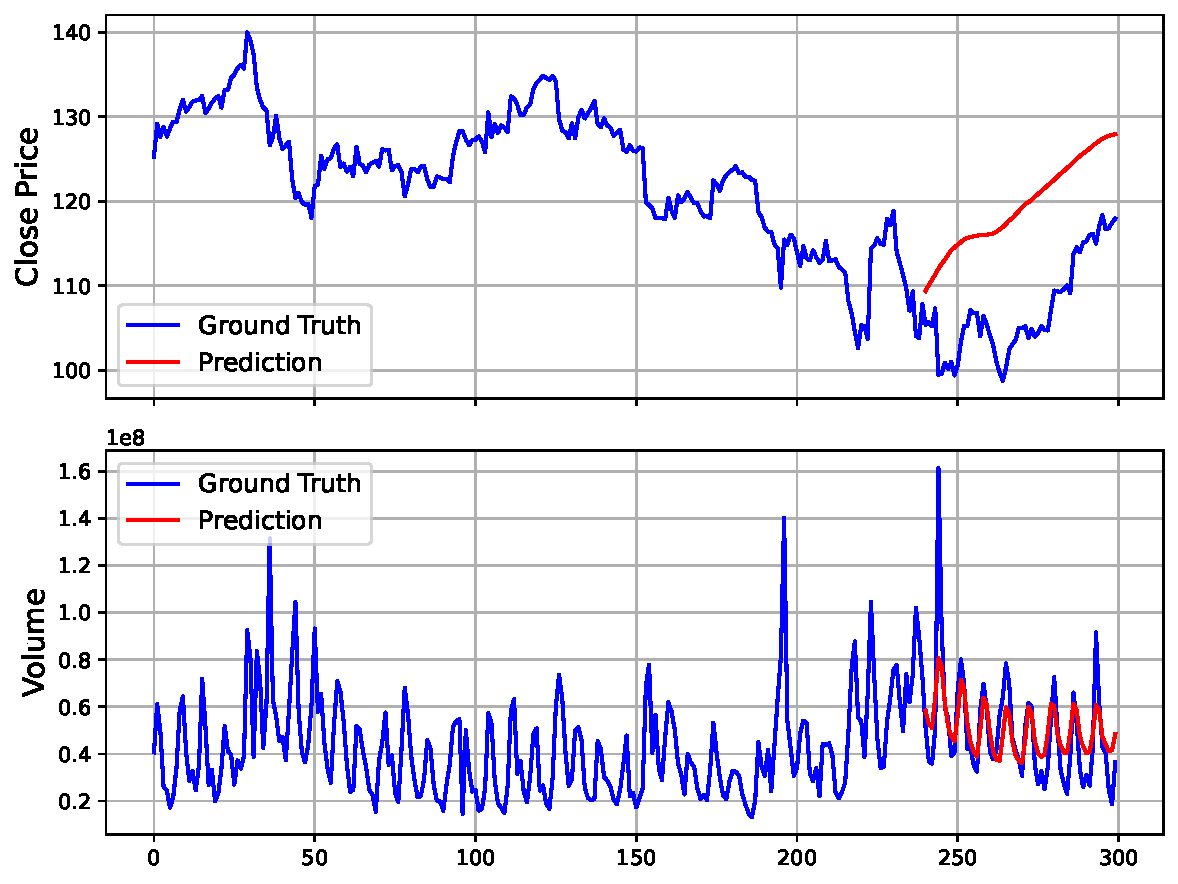
\includegraphics[width=\linewidth]{pred_imgs/pred_visualize_stock_XNAS_NVDA_60min_TimeMOE_large.pdf}
        \caption{$\text{TimeMOE}_{large}$}
    \end{subfigure}
    \hfill
    \begin{subfigure}[b]{0.33\textwidth}
        \centering
        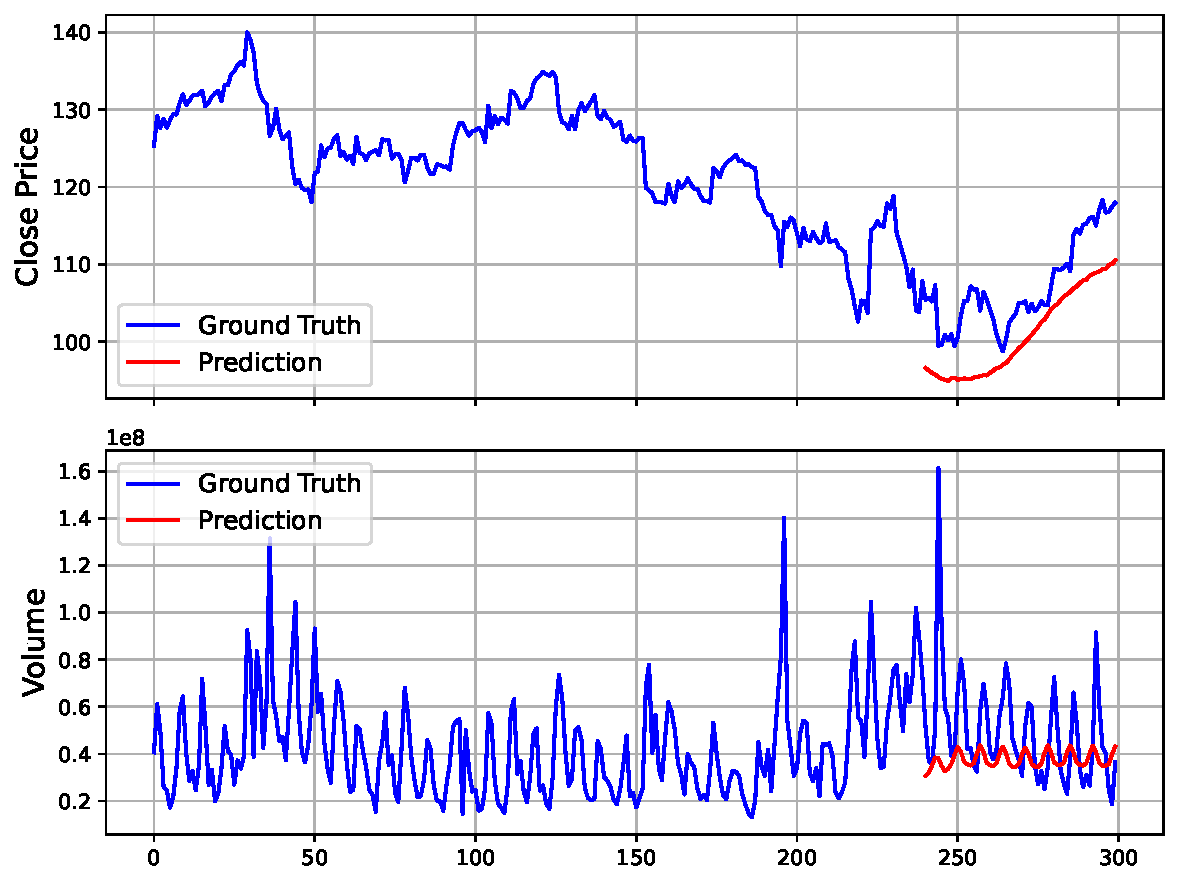
\includegraphics[width=\linewidth]{pred_imgs/pred_visualize_stock_XNAS_NVDA_60min_TimesFM.pdf}
        \caption{TimesFM}
    \end{subfigure}

    \vspace{0.1cm}

    \begin{subfigure}[b]{0.33\textwidth}
        \centering
        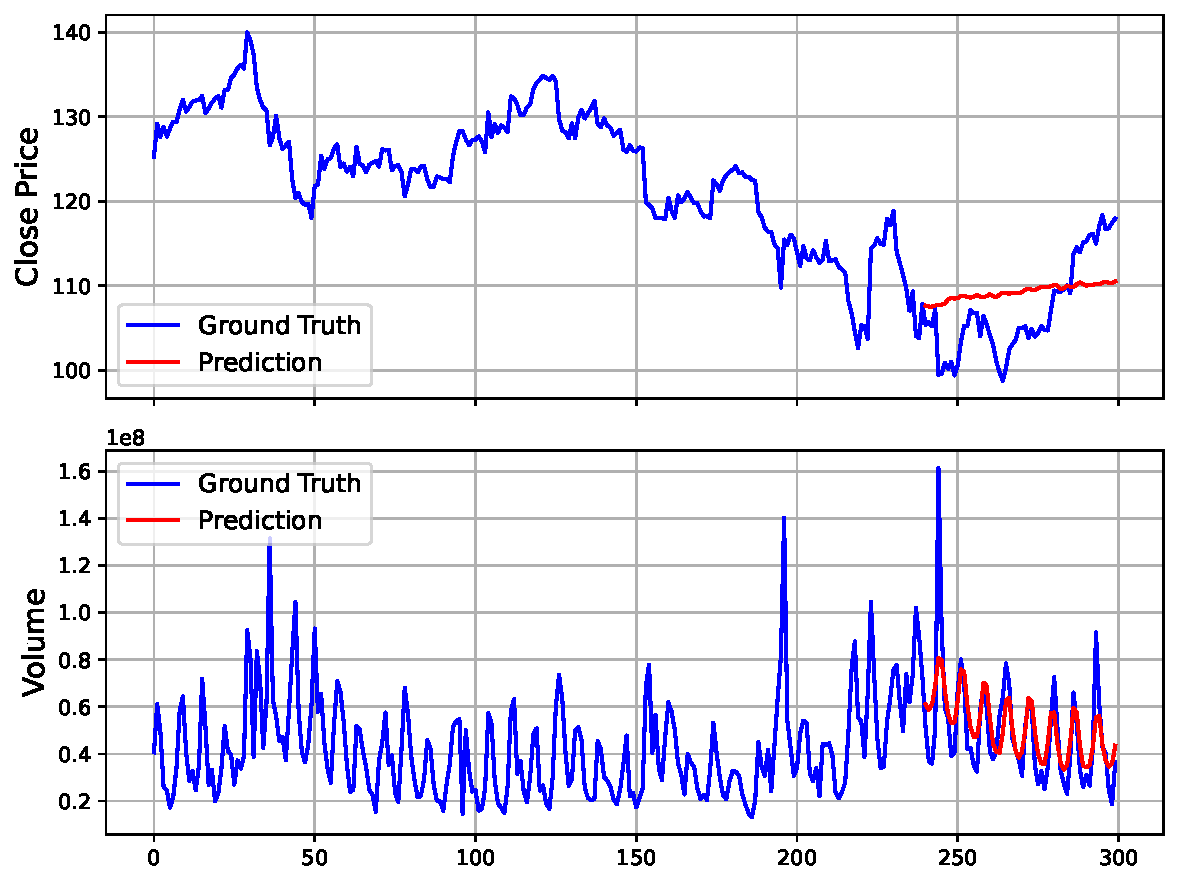
\includegraphics[width=\linewidth]{pred_imgs/pred_visualize_stock_XNAS_NVDA_60min_Chronos_small.pdf}
        \caption{$\text{Chronos}_{small}$}
    \end{subfigure}
    \hfill
    \begin{subfigure}[b]{0.33\textwidth}
        \centering
        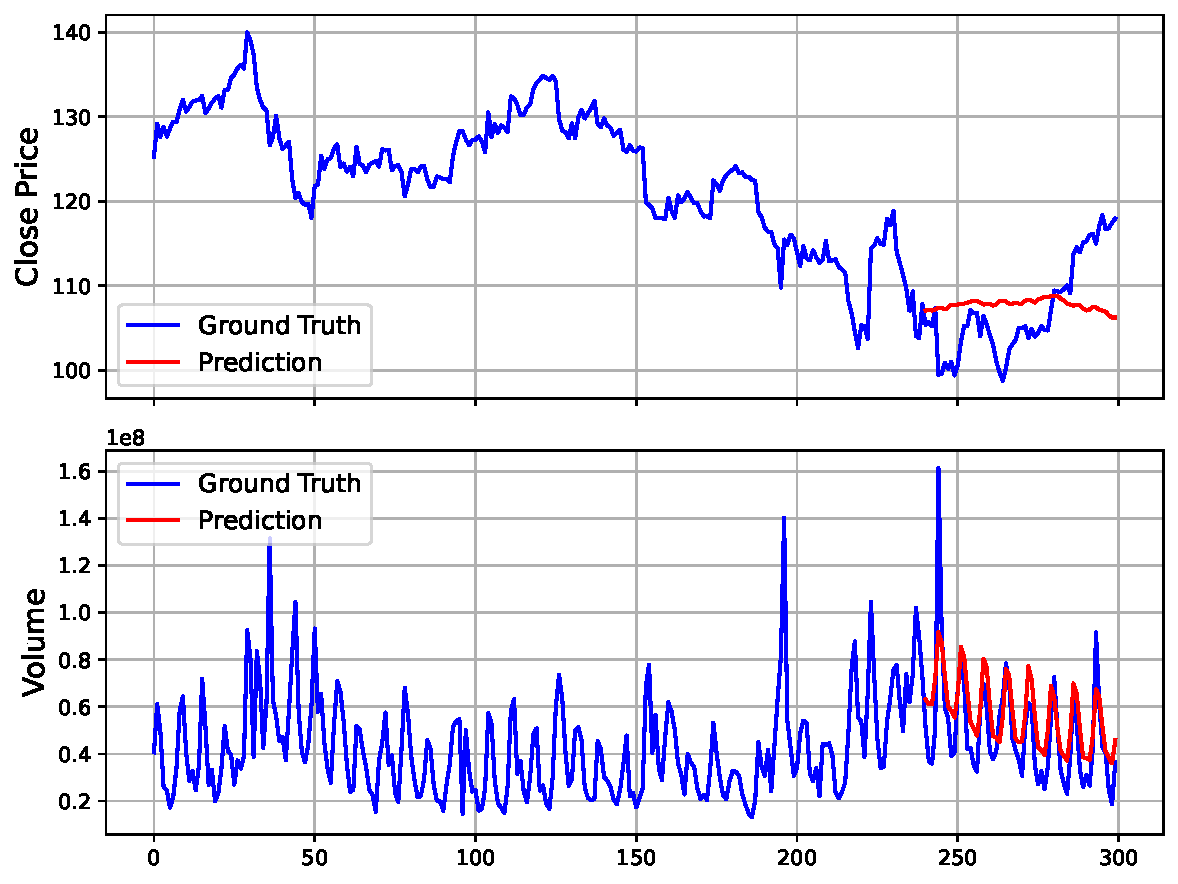
\includegraphics[width=\linewidth]{pred_imgs/pred_visualize_stock_XNAS_NVDA_60min_Chronos_base.pdf}
        \caption{$\text{Chronos}_{base}$}
    \end{subfigure}
    \hfill
    \begin{subfigure}[b]{0.33\textwidth}
        \centering
        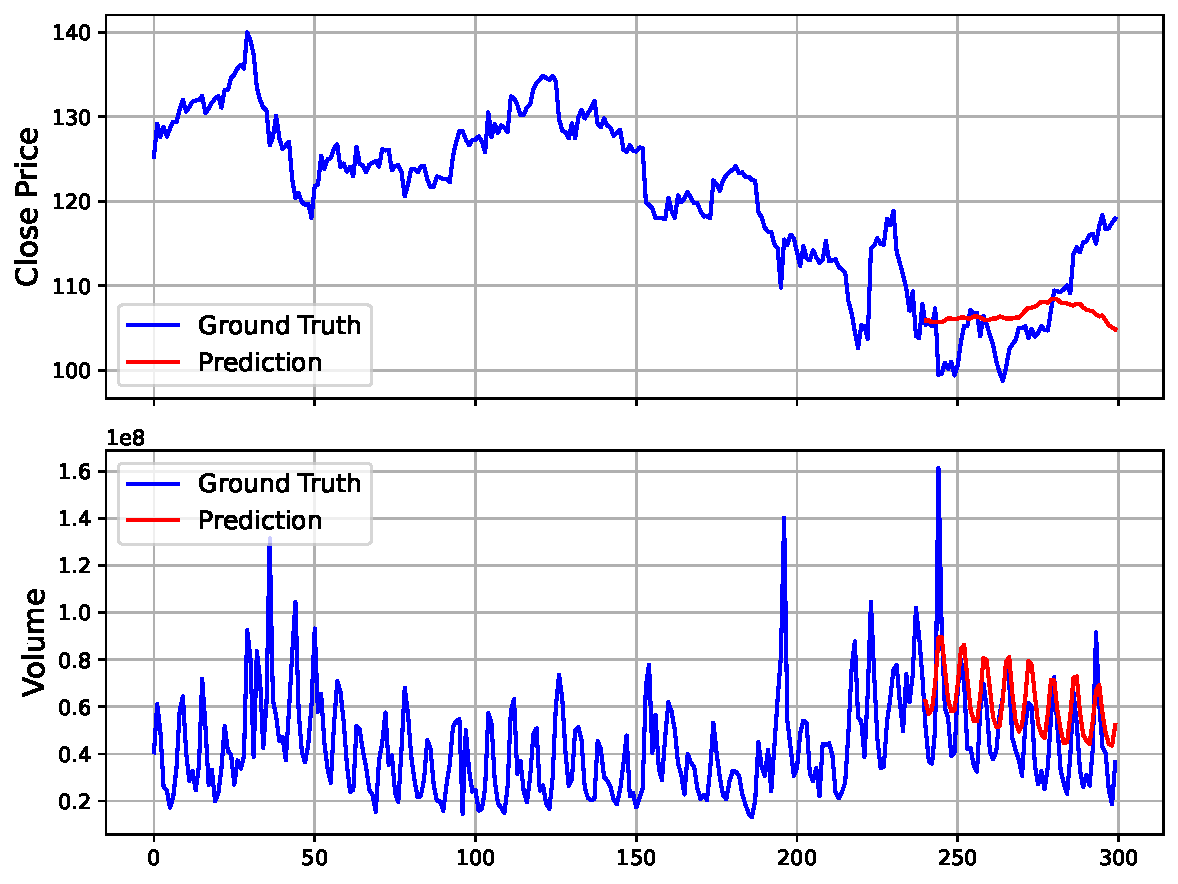
\includegraphics[width=\linewidth]{pred_imgs/pred_visualize_stock_XNAS_NVDA_60min_Chronos_large.pdf}
        \caption{$\text{Chronos}_{large}$}
    \end{subfigure}

    \vspace{0.1cm}

    \begin{subfigure}[b]{0.33\textwidth}
        \centering
        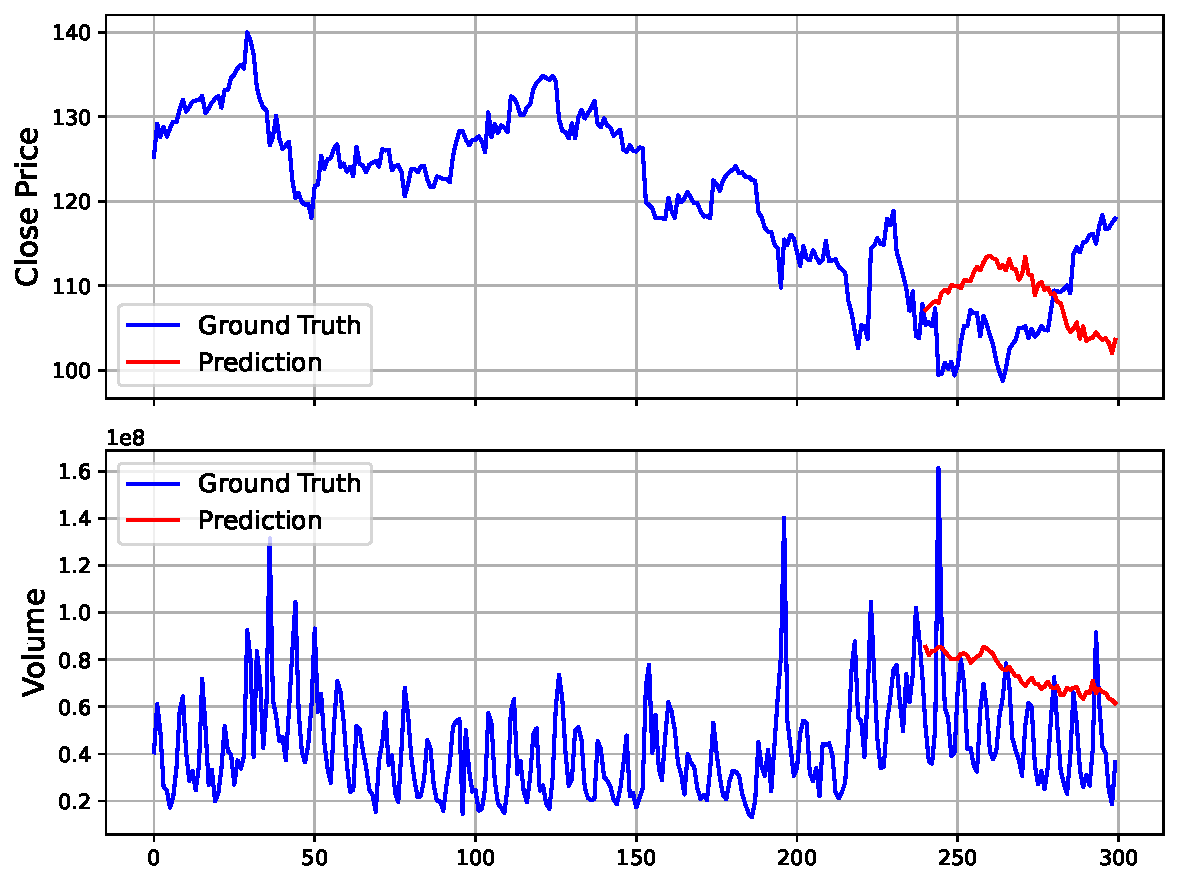
\includegraphics[width=\linewidth]{pred_imgs/pred_visualize_stock_XNAS_NVDA_60min_iTransformer.pdf}
        \caption{iTransformer}
    \end{subfigure}
    \hfill
    \begin{subfigure}[b]{0.33\textwidth}
        \centering
        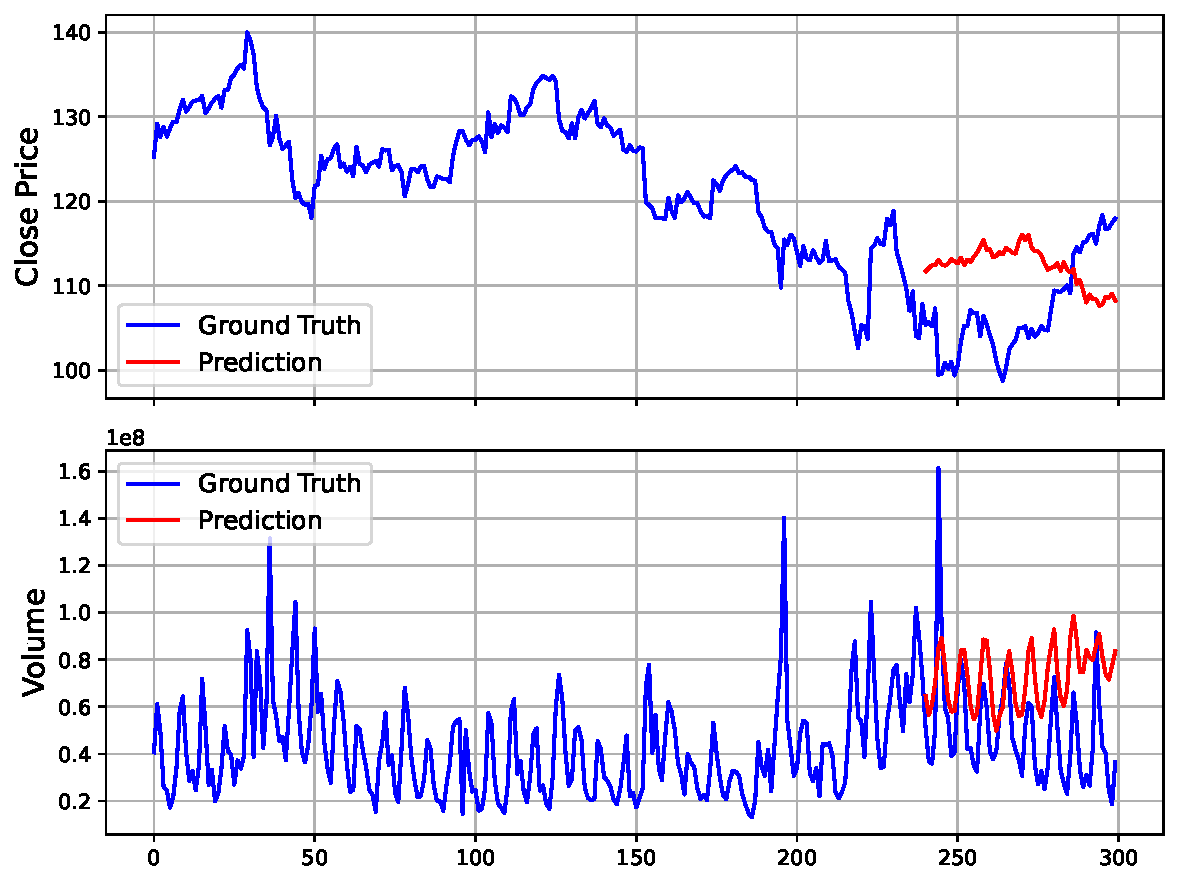
\includegraphics[width=\linewidth]{pred_imgs/pred_visualize_stock_XNAS_NVDA_60min_DLinear.pdf}
        \caption{DLinear}
    \end{subfigure}
    \hfill
    \begin{subfigure}[b]{0.33\textwidth}
        \centering
        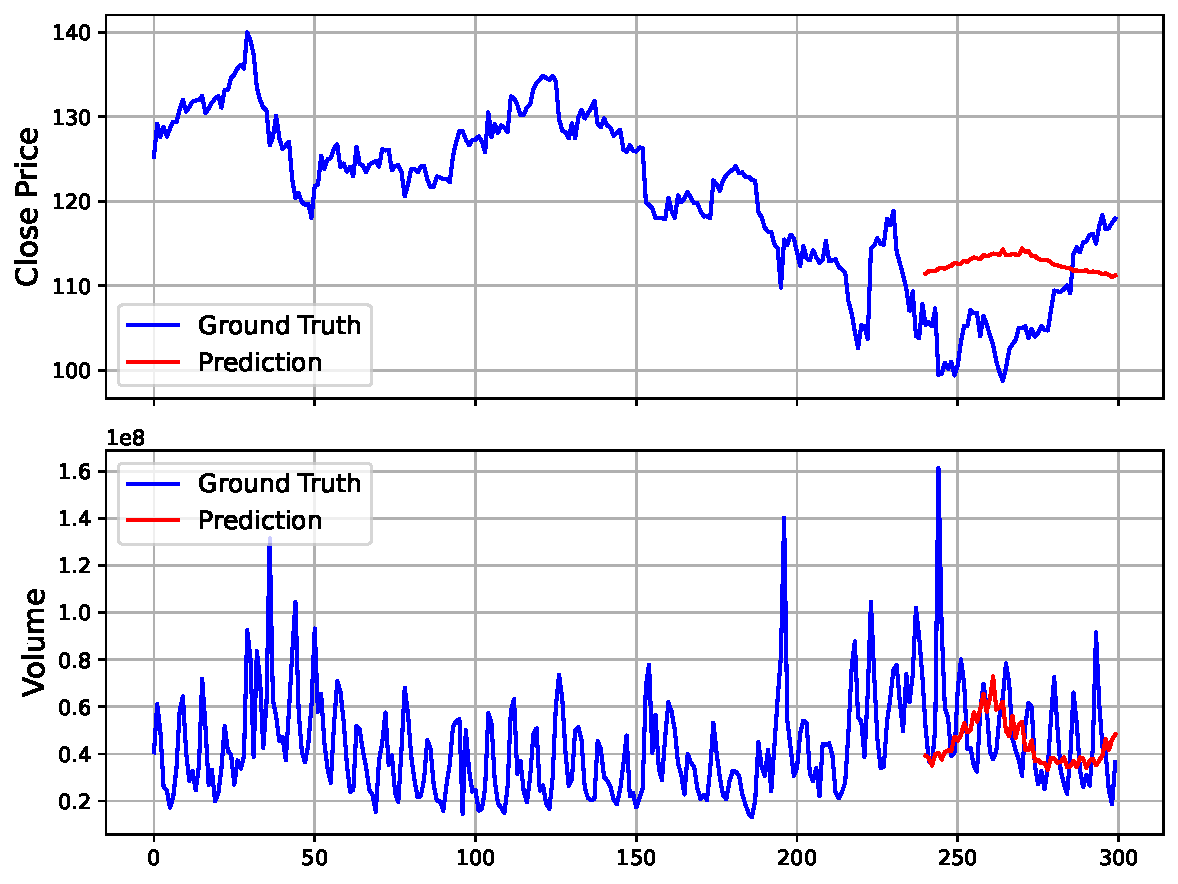
\includegraphics[width=\linewidth]{pred_imgs/pred_visualize_stock_XNAS_NVDA_60min_TimesNet.pdf}
        \caption{TimesNet}
    \end{subfigure}

    \caption{1시간 K-line 데이터를 기반으로 한 NVIDIA (NASDAQ: NVDA)의 `Close Price'와 `Volume' 예측 결과. 모델은 240스텝 look-back 윈도우를 사용하여 60스텝 horizon을 예측한다. \textcolor{blue}{Blue} 선은 정답값을 나타내고 \textcolor{red}{red} 선은 모델의 예측값을 나타낸다.}
    \label{fig:pred_case_3}
\end{figure*}


\begin{figure*}[ht]
    \centering

    \begin{subfigure}[b]{0.33\textwidth}
        \centering
        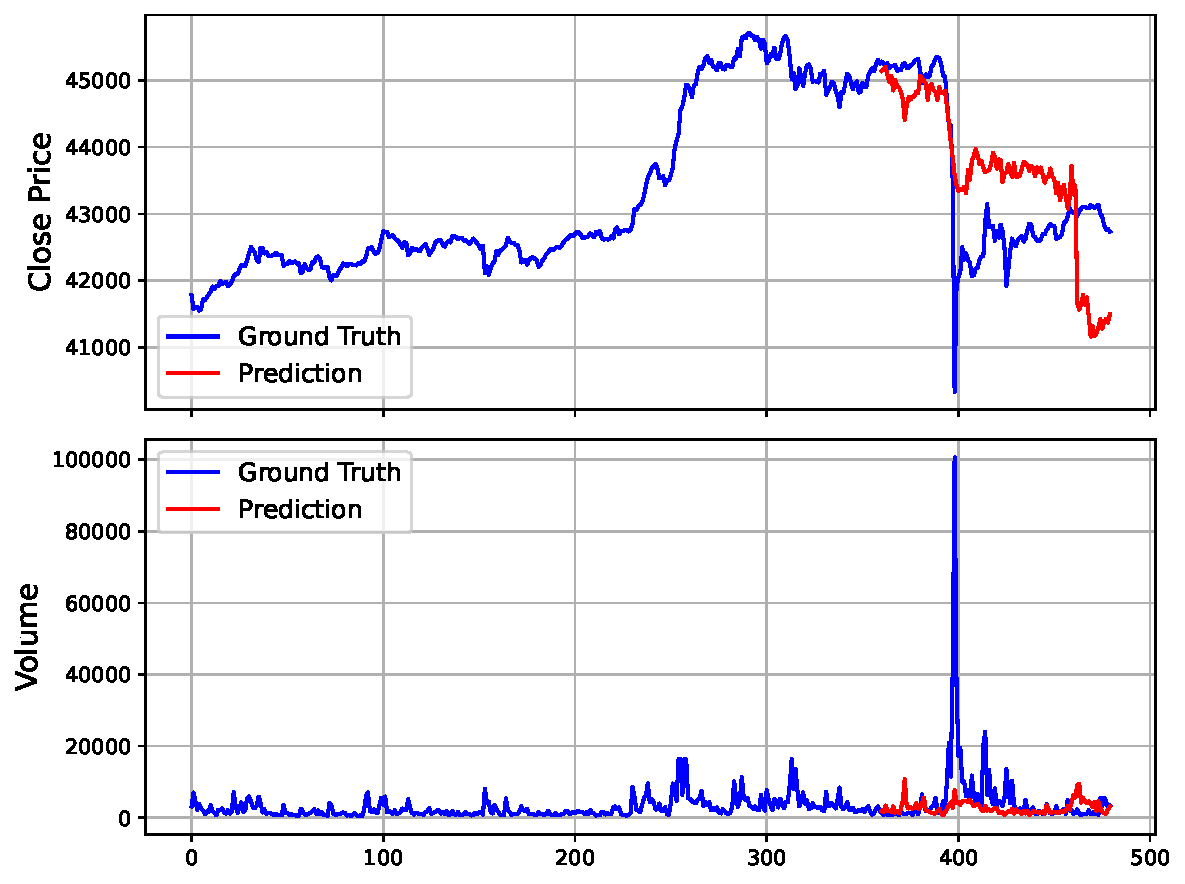
\includegraphics[width=\linewidth]{pred_imgs/pred_visualize_crypto_BTCUSDT_15min_Kronos_small.pdf}
        \caption{$\text{Kronos}_{small}$}
    \end{subfigure}
    \hfill
    \begin{subfigure}[b]{0.33\textwidth}
        \centering
        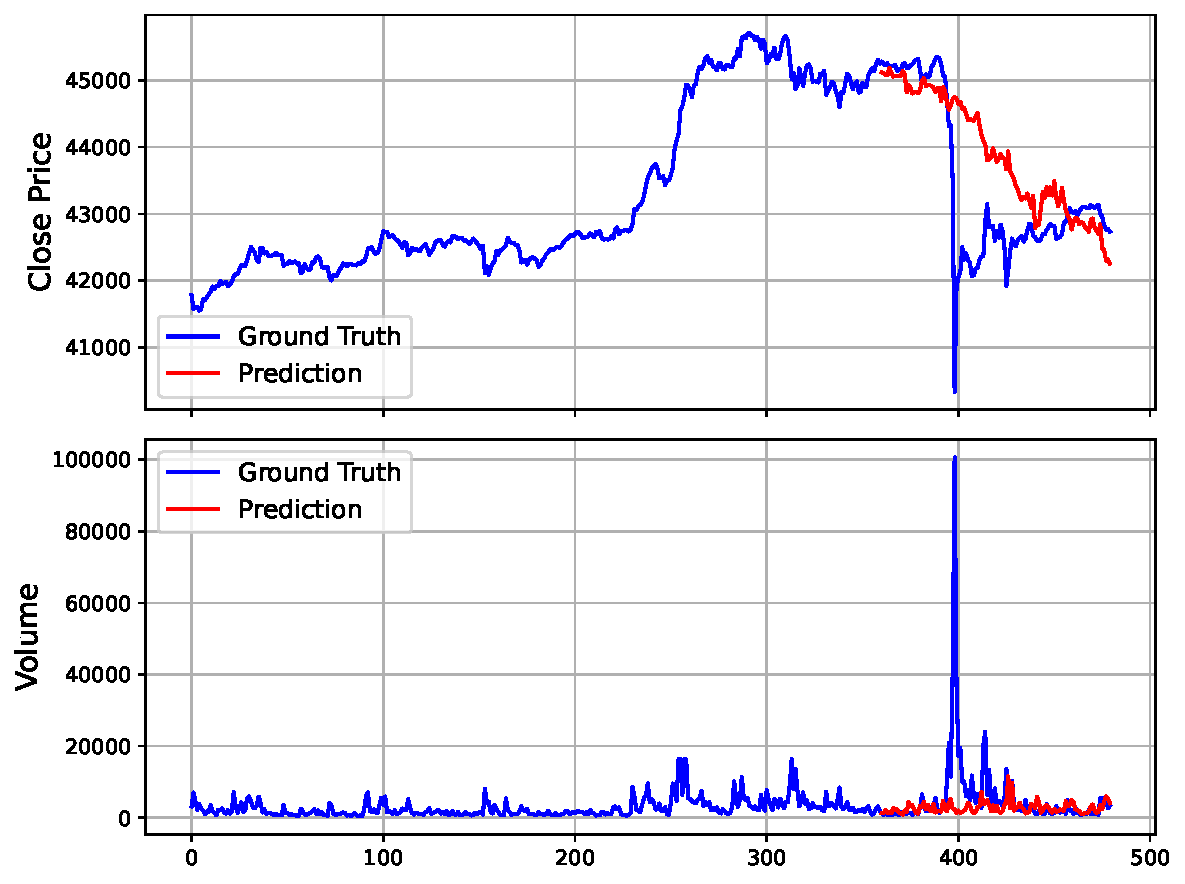
\includegraphics[width=\linewidth]{pred_imgs/pred_visualize_crypto_BTCUSDT_15min_Kronos_base.pdf}
        \caption{$\text{Kronos}_{base}$}
    \end{subfigure}
    \hfill
    \begin{subfigure}[b]{0.33\textwidth}
        \centering
        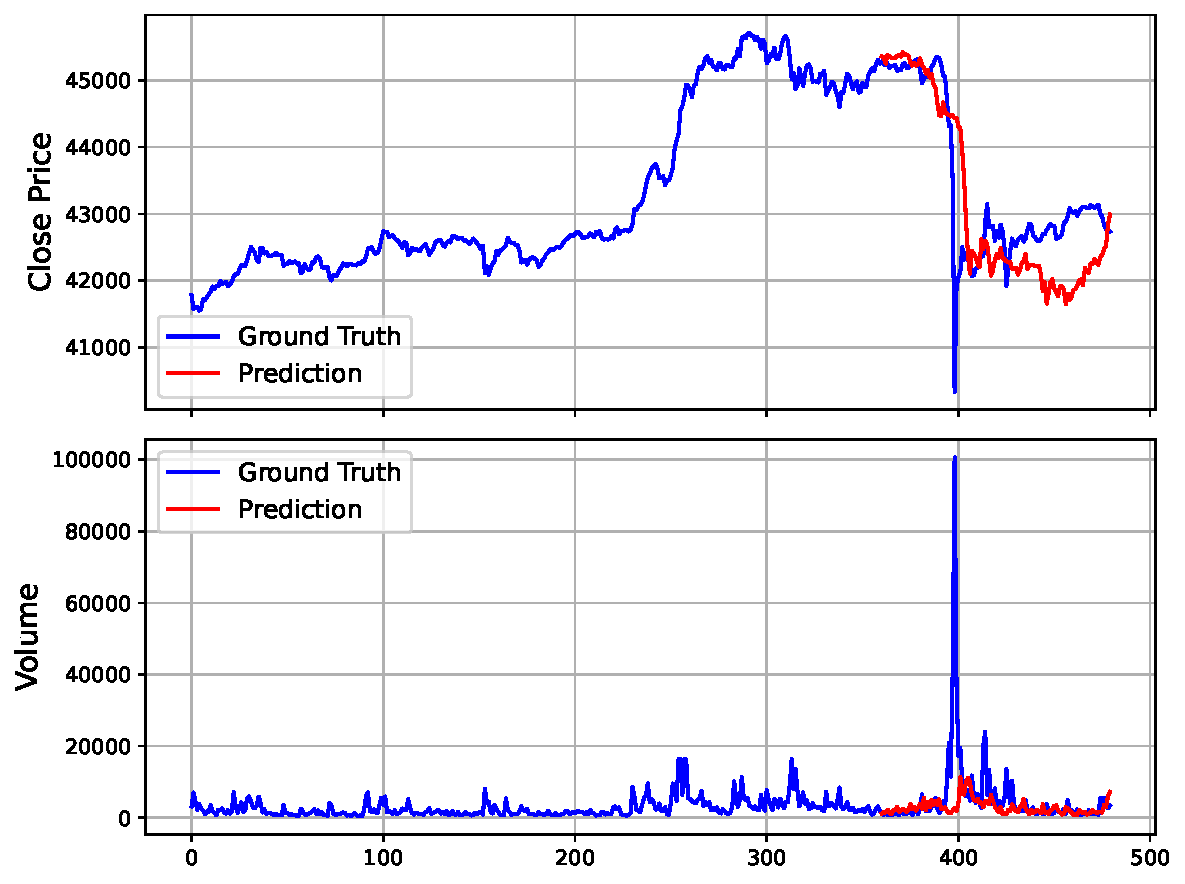
\includegraphics[width=\linewidth]{pred_imgs/pred_visualize_crypto_BTCUSDT_15min_Kronos_large.pdf}
        \caption{$\text{Kronos}_{large}$}
    \end{subfigure}

    \vspace{0.1cm}

    \begin{subfigure}[b]{0.33\textwidth}
        \centering
        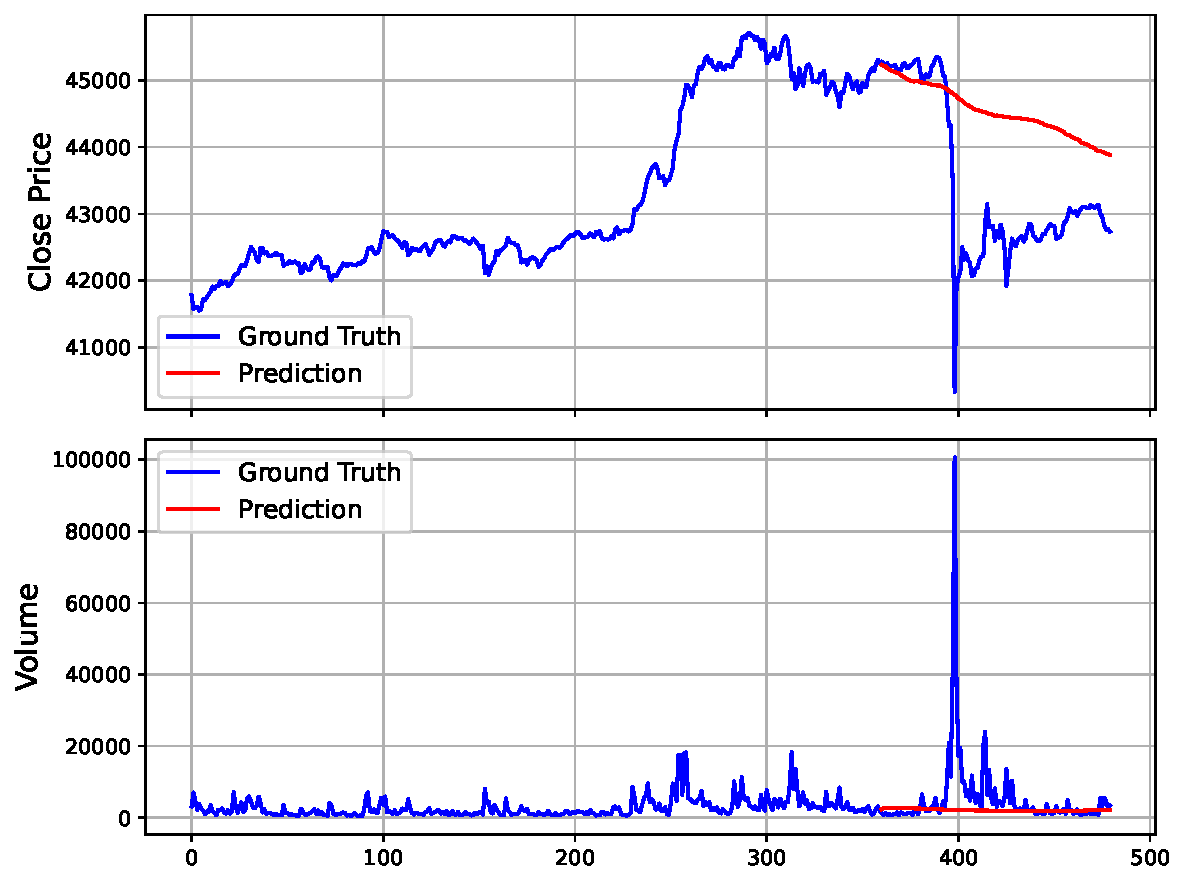
\includegraphics[width=\linewidth]{pred_imgs/pred_visualize_crypto_BTCUSDT_15min_TimeMOE_small.pdf}
        \caption{$\text{TimeMOE}_{small}$}
    \end{subfigure}
    \hfill
    \begin{subfigure}[b]{0.33\textwidth}
        \centering
        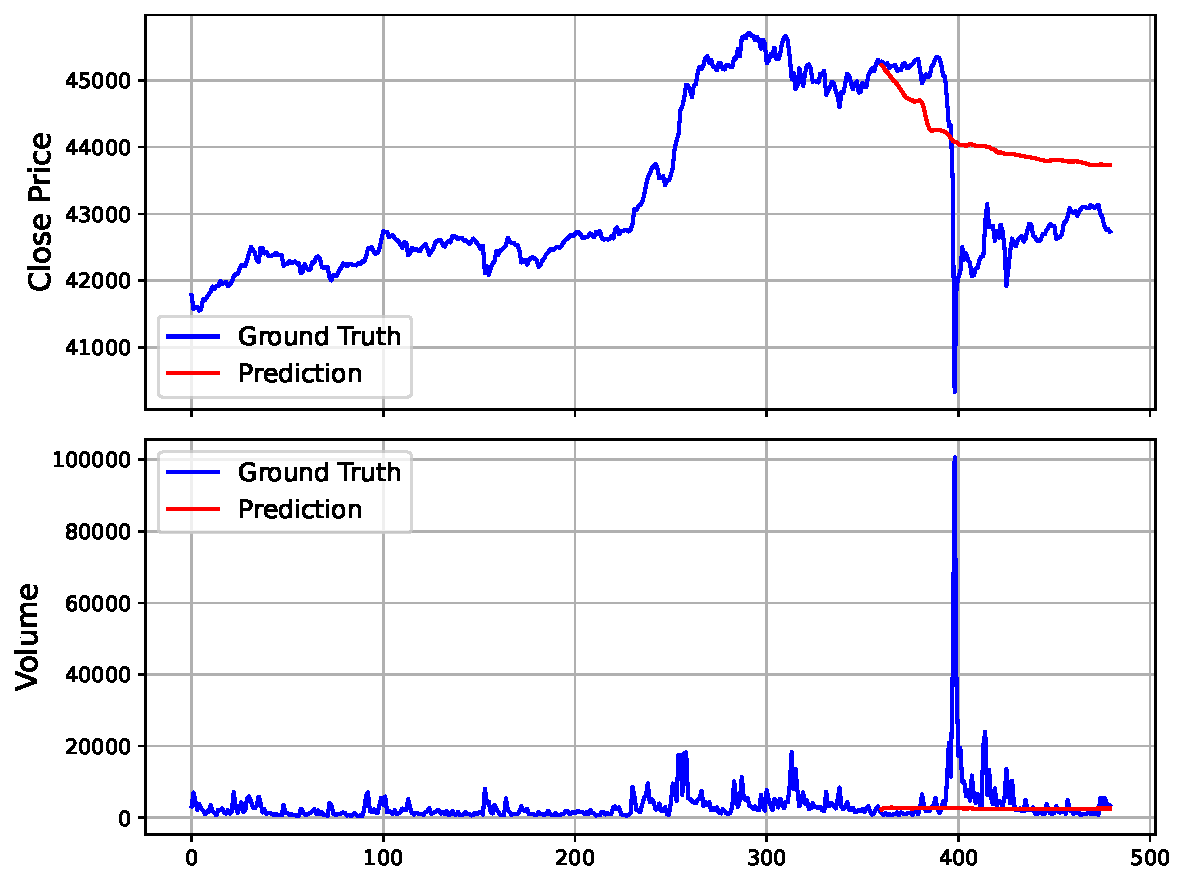
\includegraphics[width=\linewidth]{pred_imgs/pred_visualize_crypto_BTCUSDT_15min_TimeMOE_large.pdf}
        \caption{$\text{TimeMOE}_{large}$}
    \end{subfigure}
    \hfill
    \begin{subfigure}[b]{0.33\textwidth}
        \centering
        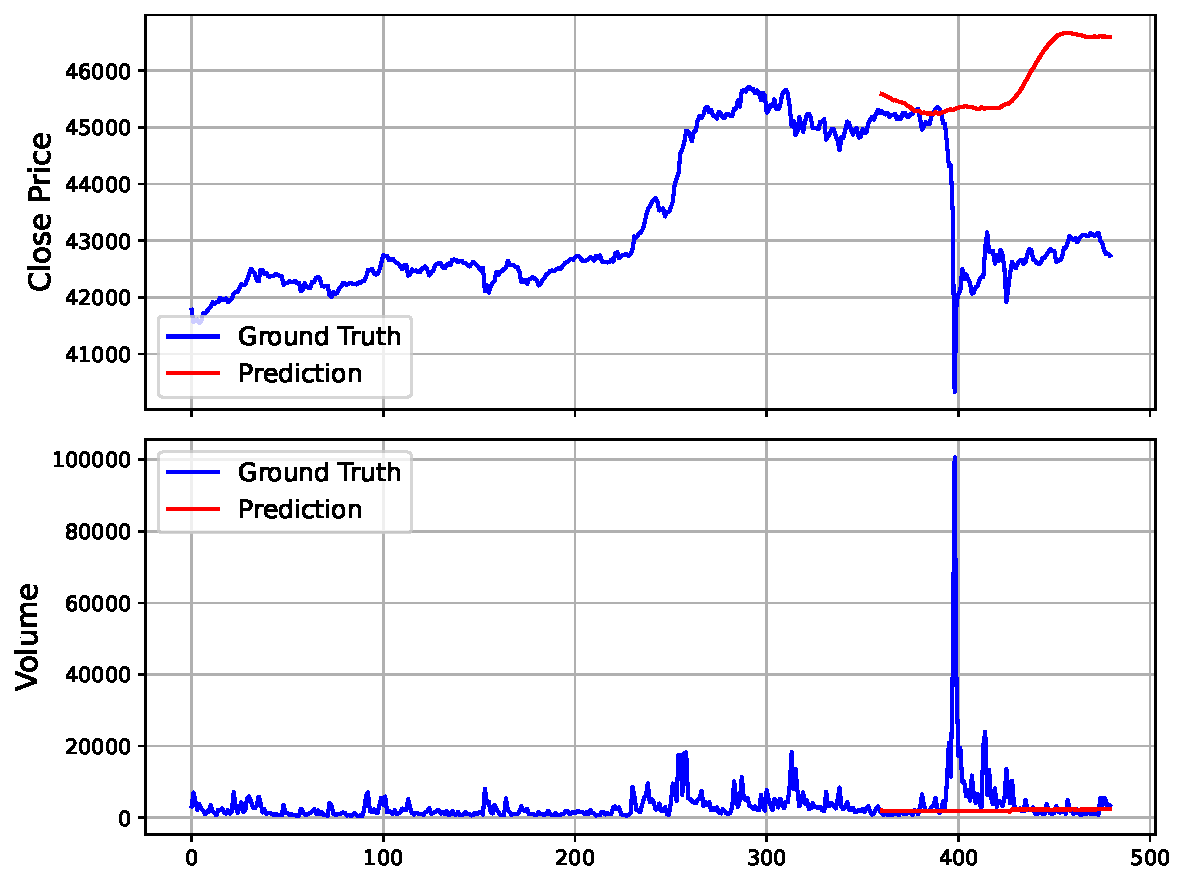
\includegraphics[width=\linewidth]{pred_imgs/pred_visualize_crypto_BTCUSDT_15min_TimesFM.pdf}
        \caption{TimesFM}
    \end{subfigure}

    \vspace{0.1cm}

    \begin{subfigure}[b]{0.33\textwidth}
        \centering
        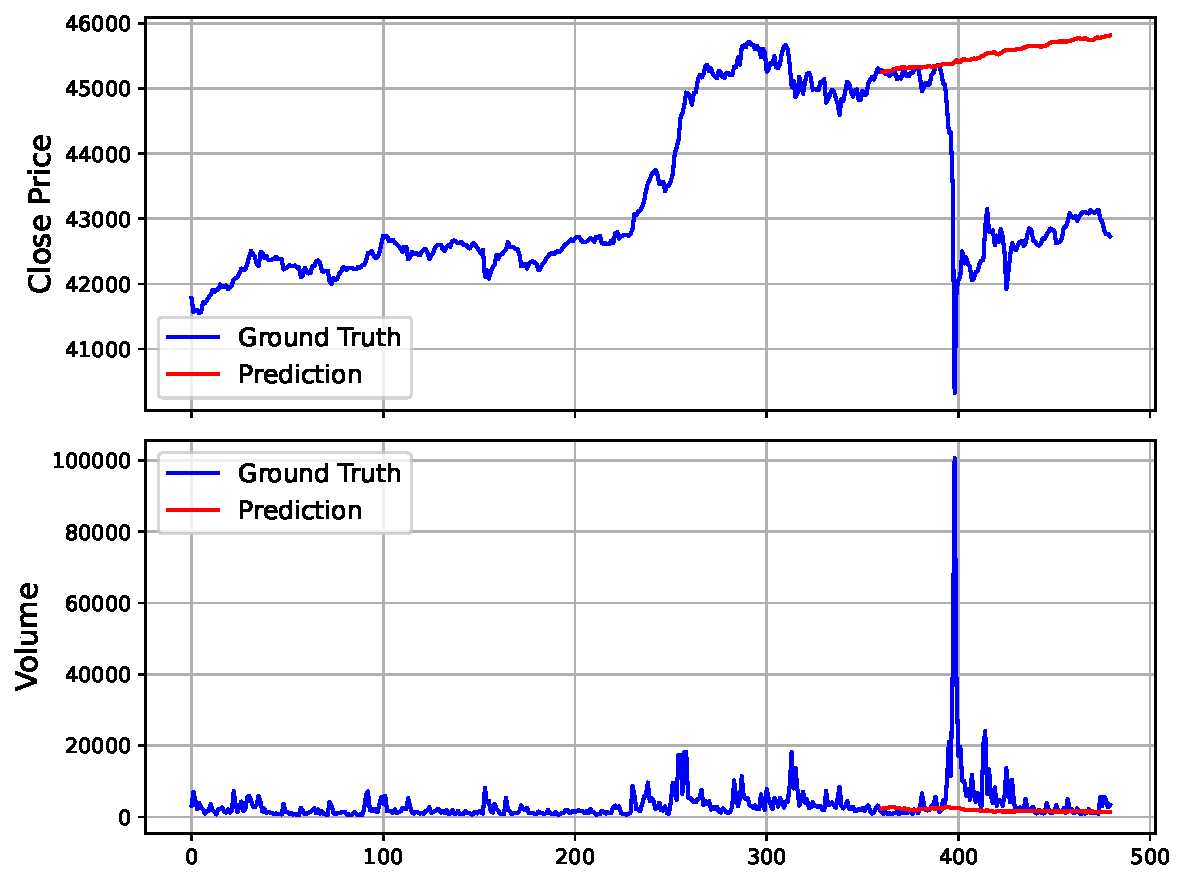
\includegraphics[width=\linewidth]{pred_imgs/pred_visualize_crypto_BTCUSDT_15min_Chronos_small.pdf}
        \caption{$\text{Chronos}_{small}$}
    \end{subfigure}
    \hfill
    \begin{subfigure}[b]{0.33\textwidth}
        \centering
        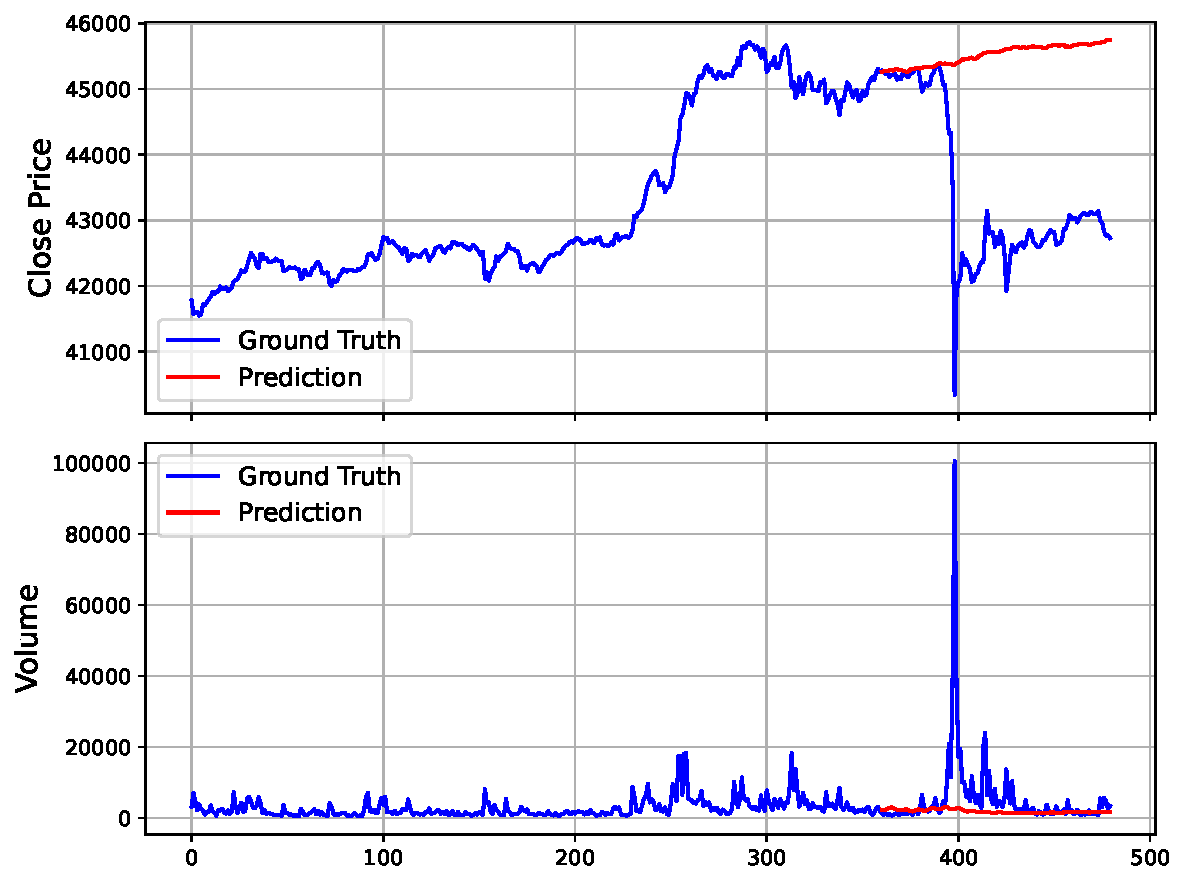
\includegraphics[width=\linewidth]{pred_imgs/pred_visualize_crypto_BTCUSDT_15min_Chronos_base.pdf}
        \caption{$\text{Chronos}_{base}$}
    \end{subfigure}
    \hfill
    \begin{subfigure}[b]{0.33\textwidth}
        \centering
        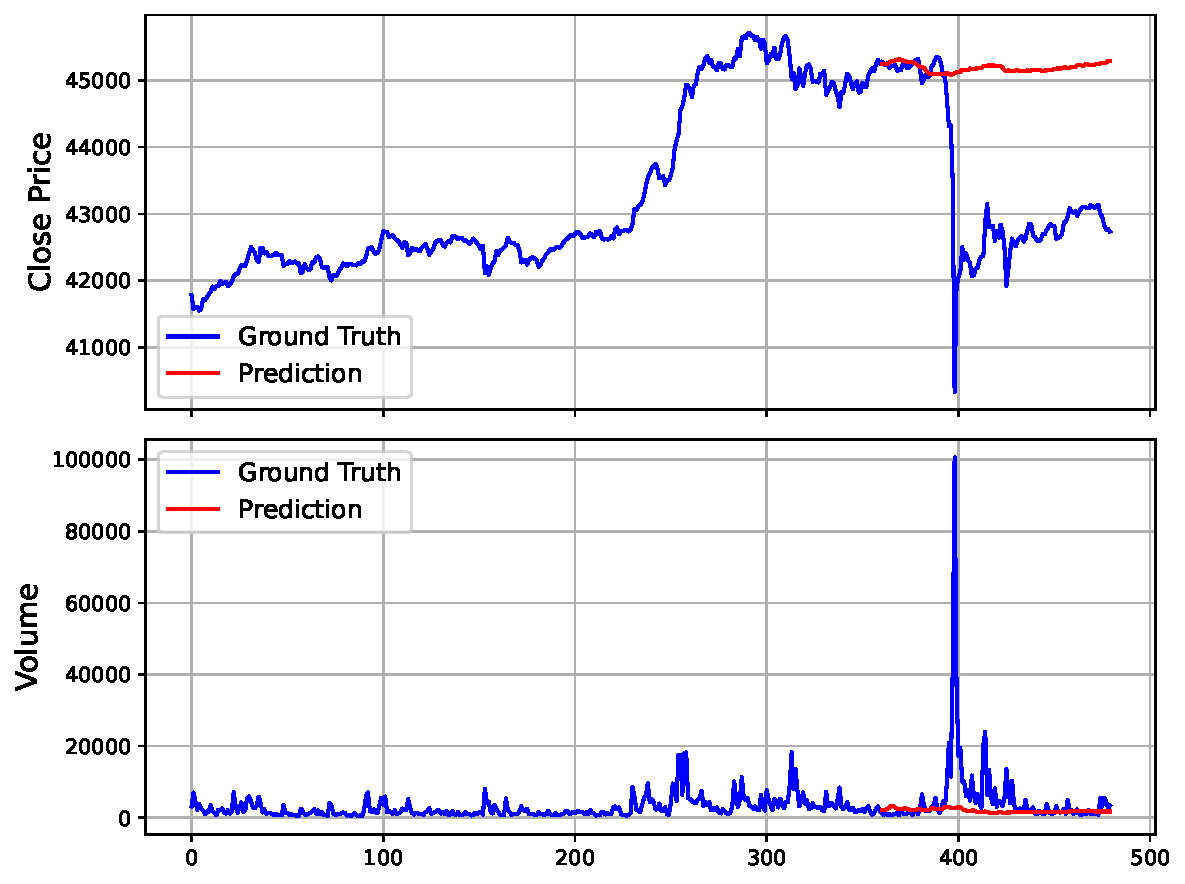
\includegraphics[width=\linewidth]{pred_imgs/pred_visualize_crypto_BTCUSDT_15min_Chronos_large.pdf}
        \caption{$\text{Chronos}_{large}$}
    \end{subfigure}

    \vspace{0.1cm}

    \begin{subfigure}[b]{0.33\textwidth}
        \centering
        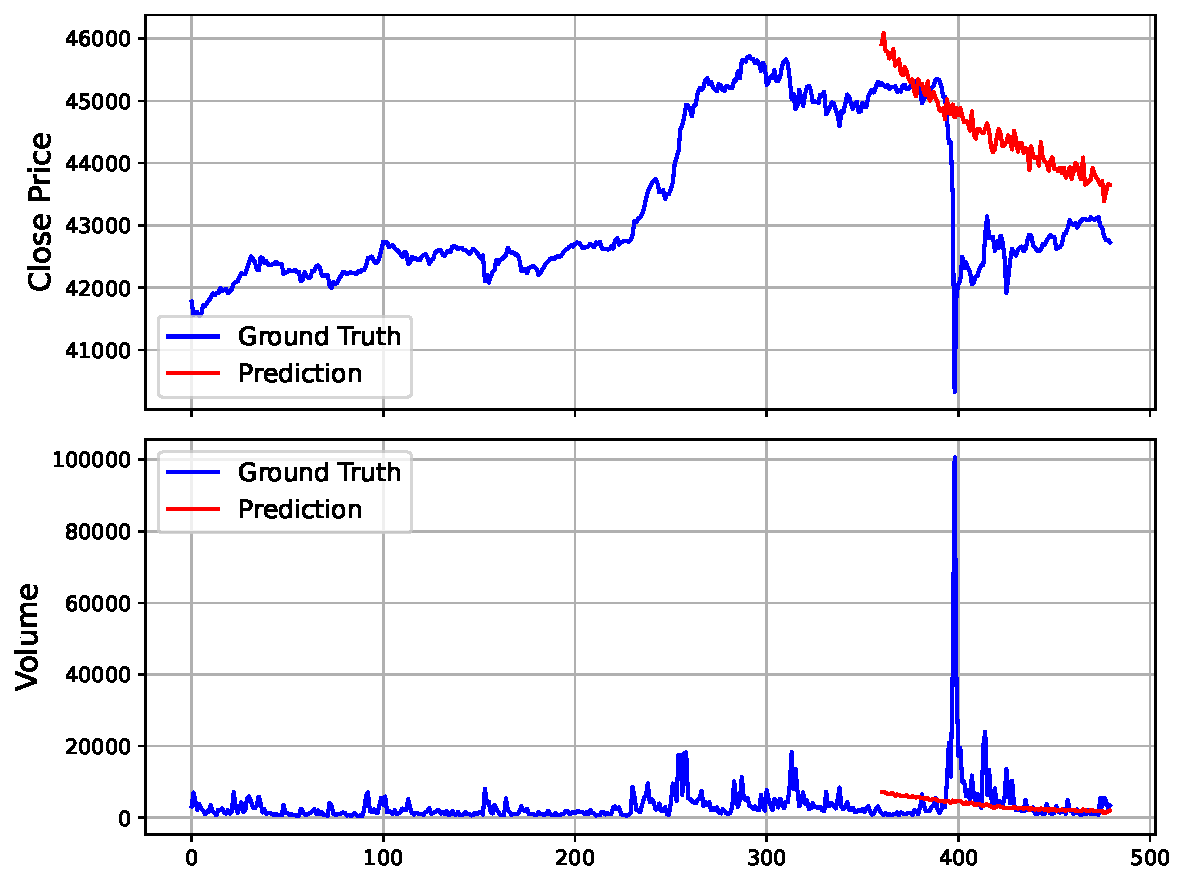
\includegraphics[width=\linewidth]{pred_imgs/pred_visualize_crypto_BTCUSDT_15min_iTransformer.pdf}
        \caption{iTransformer}
    \end{subfigure}
    \hfill
    \begin{subfigure}[b]{0.33\textwidth}
        \centering
        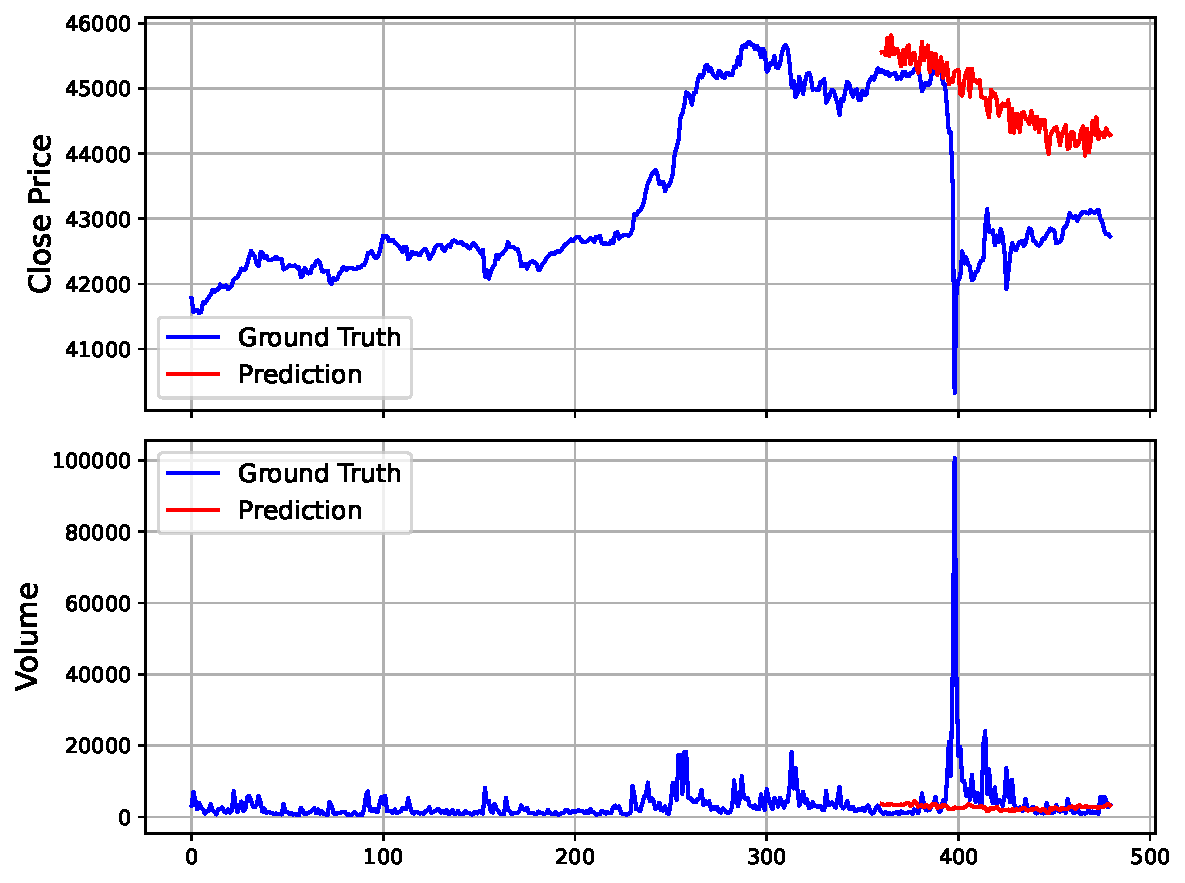
\includegraphics[width=\linewidth]{pred_imgs/pred_visualize_crypto_BTCUSDT_15min_DLinear.pdf}
        \caption{DLinear}
    \end{subfigure}
    \hfill
    \begin{subfigure}[b]{0.33\textwidth}
        \centering
        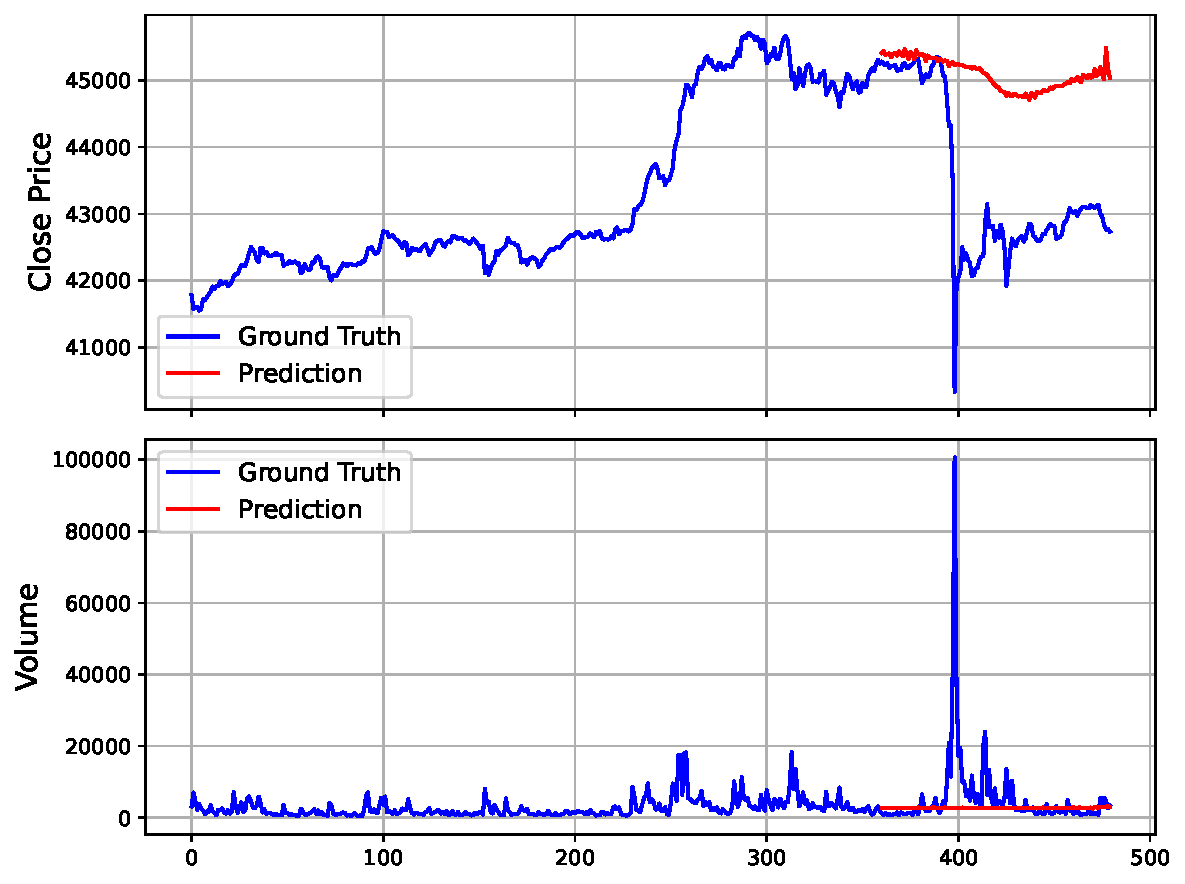
\includegraphics[width=\linewidth]{pred_imgs/pred_visualize_crypto_BTCUSDT_15min_TimesNet.pdf}
        \caption{TimesNet}
    \end{subfigure}

    \caption{15분 K-line 데이터를 기반으로 한 Binance의 BTC/USDT 무기한 계약의 `Close Price'와 `Volume' 예측 결과. 모델은 360스텝 look-back 윈도우를 사용하여 120스텝 horizon을 예측한다. \textcolor{blue}{Blue} 선은 정답값을 나타내고 \textcolor{red}{red} 선은 모델의 예측값을 나타낸다.}
    \label{fig:pred_case_4}
\end{figure*}

\begin{figure*}[ht]
    \centering

    \begin{subfigure}[b]{0.33\textwidth}
        \centering
        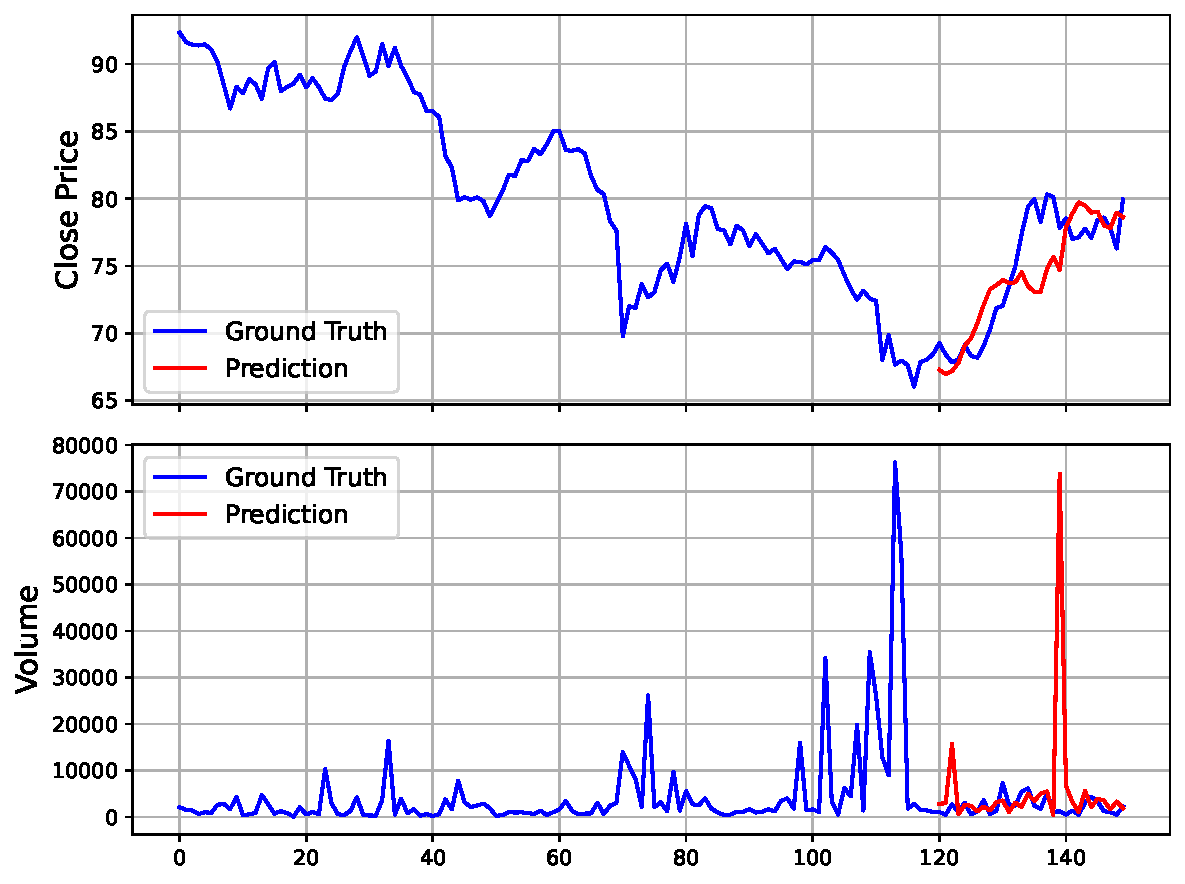
\includegraphics[width=\linewidth]{pred_imgs/pred_visualize_stock_XFRA_BMW_daily_Kronos_small.pdf}
        \caption{$\text{Kronos}_{small}$}
    \end{subfigure}
    \hfill
    \begin{subfigure}[b]{0.33\textwidth}
        \centering
        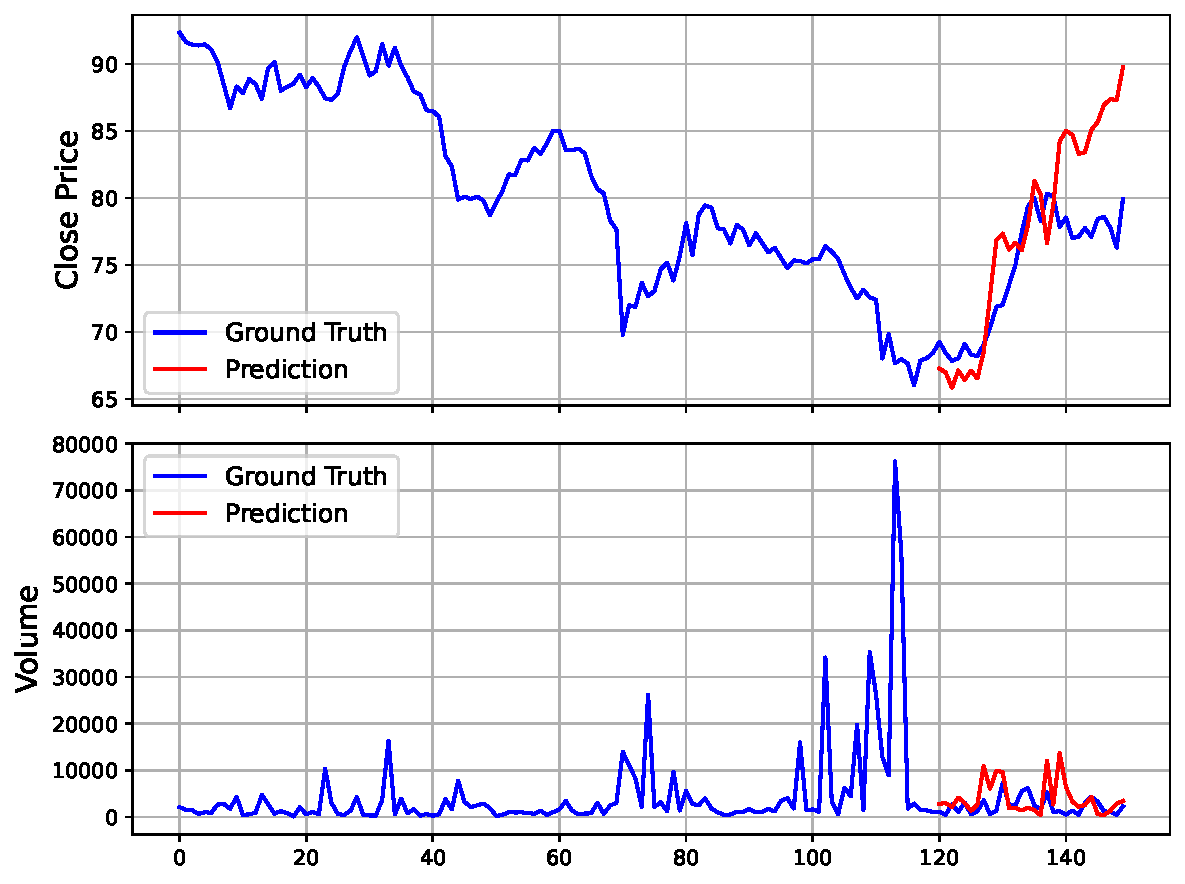
\includegraphics[width=\linewidth]{pred_imgs/pred_visualize_stock_XFRA_BMW_daily_Kronos_base.pdf}
        \caption{$\text{Kronos}_{base}$}
    \end{subfigure}
    \hfill
    \begin{subfigure}[b]{0.33\textwidth}
        \centering
        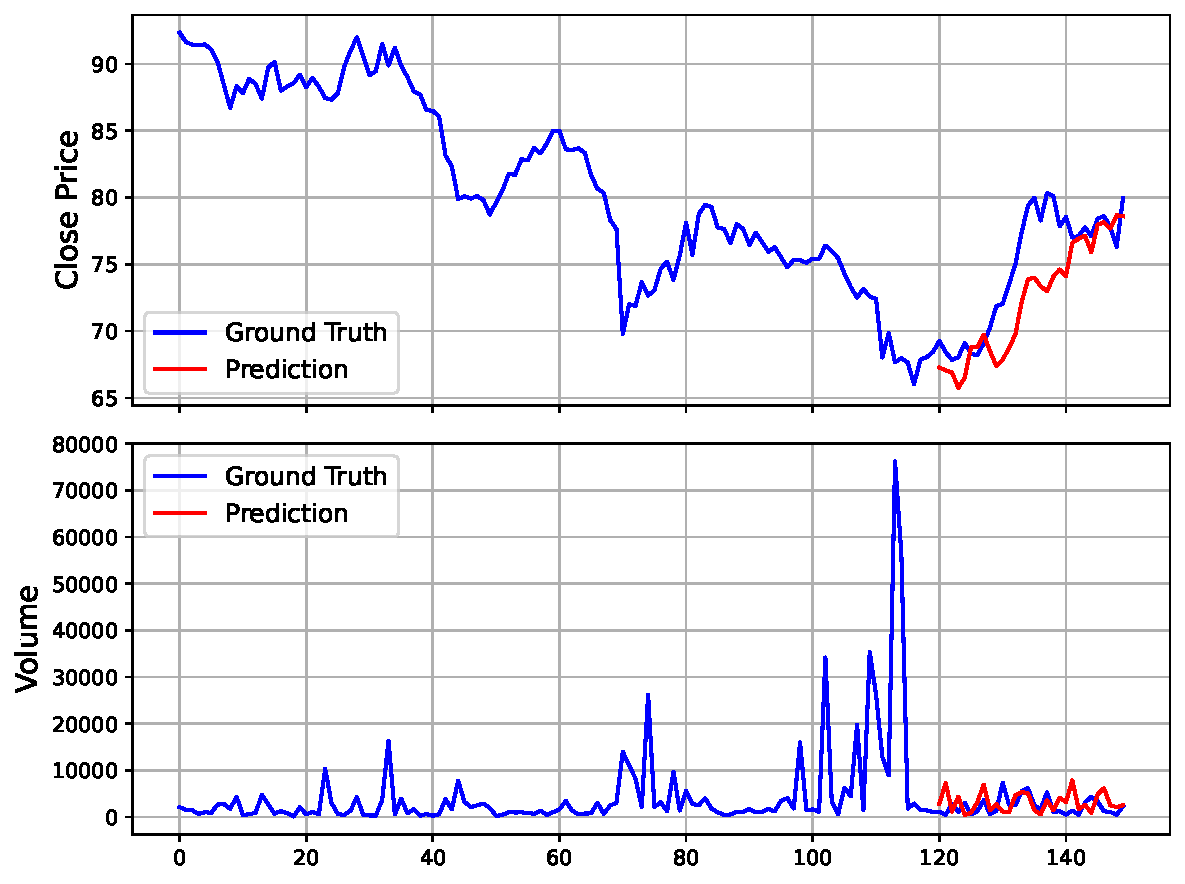
\includegraphics[width=\linewidth]{pred_imgs/pred_visualize_stock_XFRA_BMW_daily_Kronos_large.pdf}
        \caption{$\text{Kronos}_{large}$}
    \end{subfigure}

    \vspace{0.1cm}

    \begin{subfigure}[b]{0.33\textwidth}
        \centering
        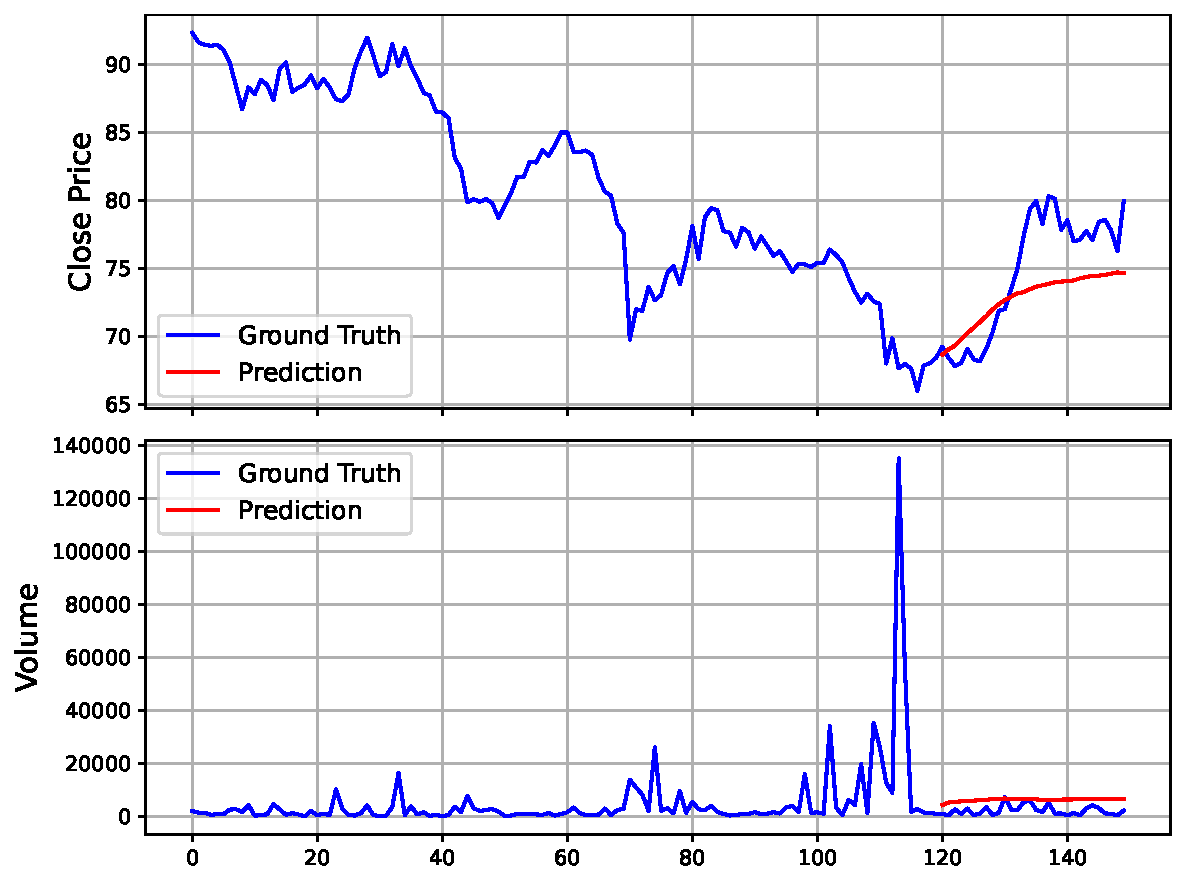
\includegraphics[width=\linewidth]{pred_imgs/pred_visualize_stock_XFRA_BMW_daily_TimeMOE_small.pdf}
        \caption{$\text{TimeMOE}_{small}$}
    \end{subfigure}
    \hfill
    \begin{subfigure}[b]{0.33\textwidth}
        \centering
        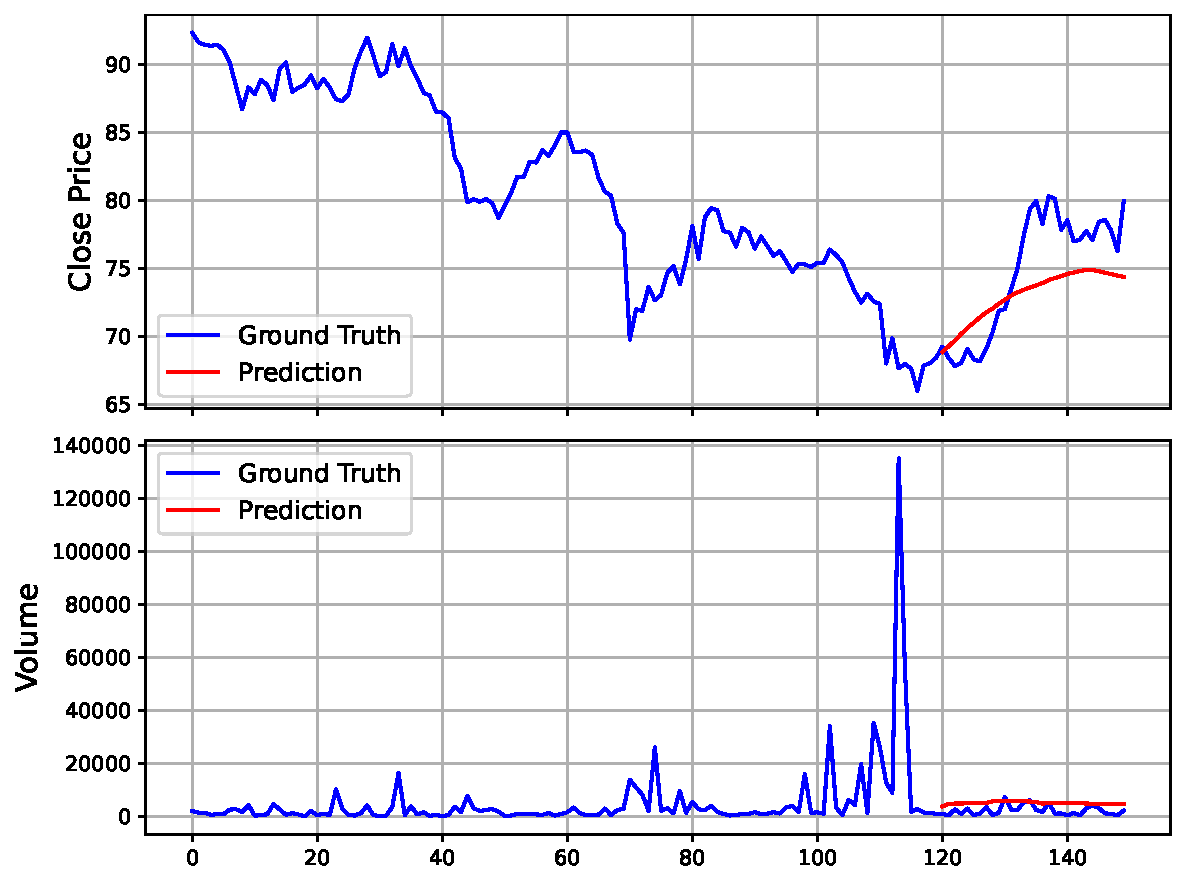
\includegraphics[width=\linewidth]{pred_imgs/pred_visualize_stock_XFRA_BMW_daily_TimeMOE_large.pdf}
        \caption{$\text{TimeMOE}_{large}$}
    \end{subfigure}
    \hfill
    \begin{subfigure}[b]{0.33\textwidth}
        \centering
        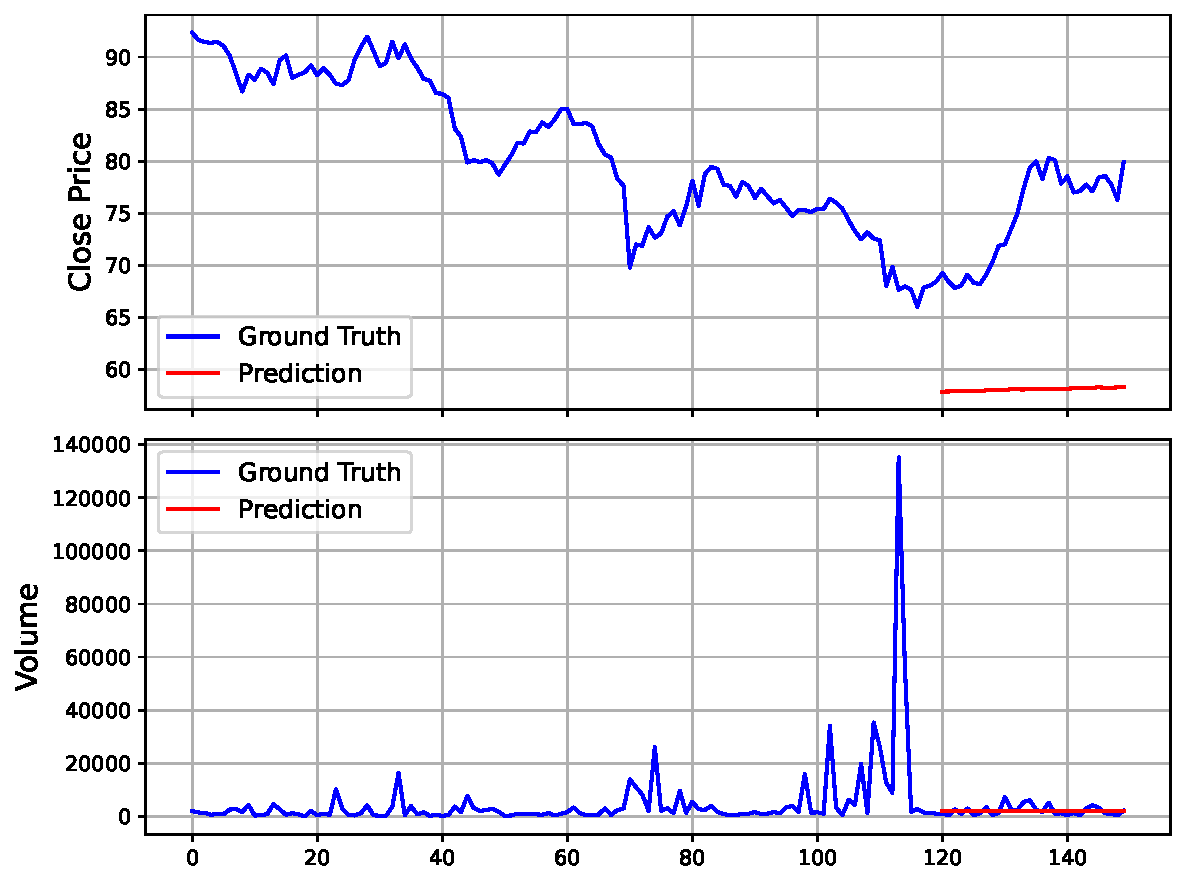
\includegraphics[width=\linewidth]{pred_imgs/pred_visualize_stock_XFRA_BMW_daily_TimesFM.pdf}
        \caption{TimesFM}
    \end{subfigure}

    \vspace{0.1cm}

    \begin{subfigure}[b]{0.33\textwidth}
        \centering
        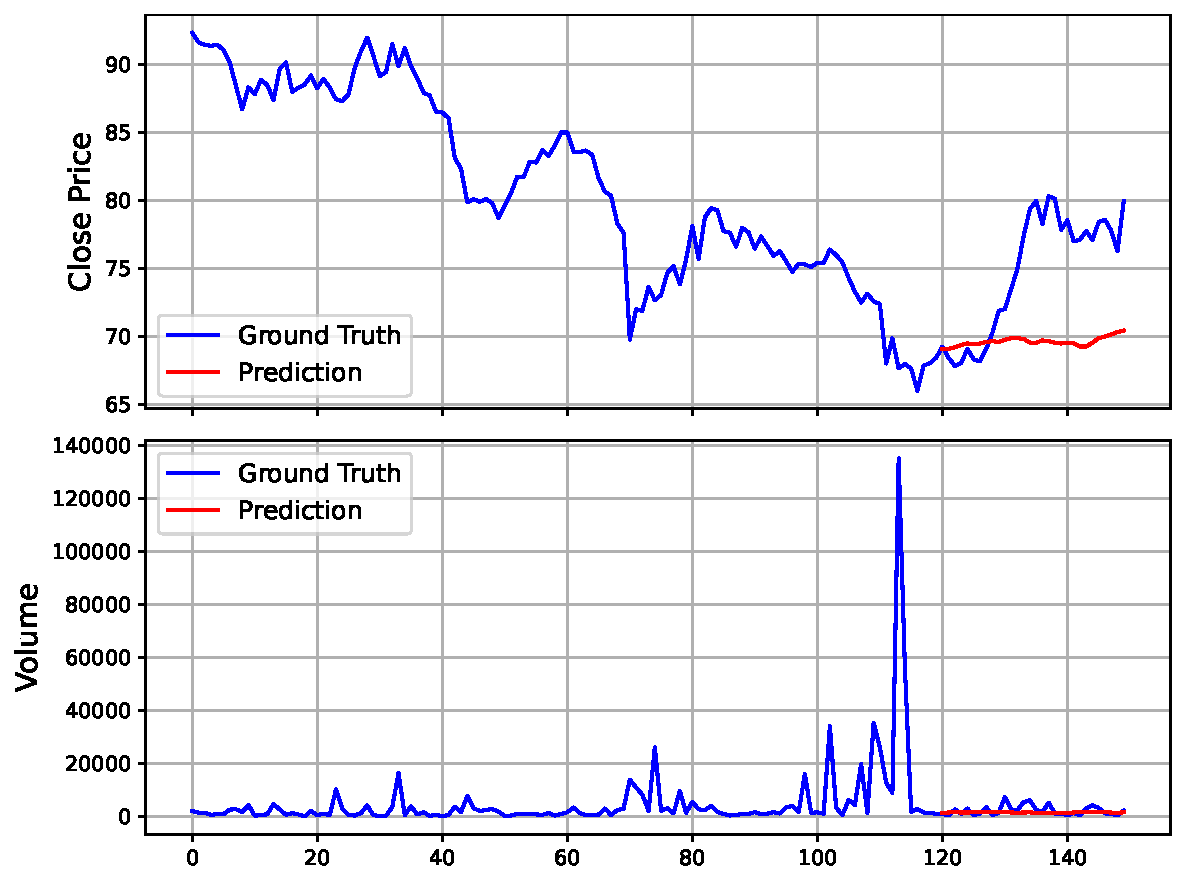
\includegraphics[width=\linewidth]{pred_imgs/pred_visualize_stock_XFRA_BMW_daily_Chronos_small.pdf}
        \caption{$\text{Chronos}_{small}$}
    \end{subfigure}
    \hfill
    \begin{subfigure}[b]{0.33\textwidth}
        \centering
        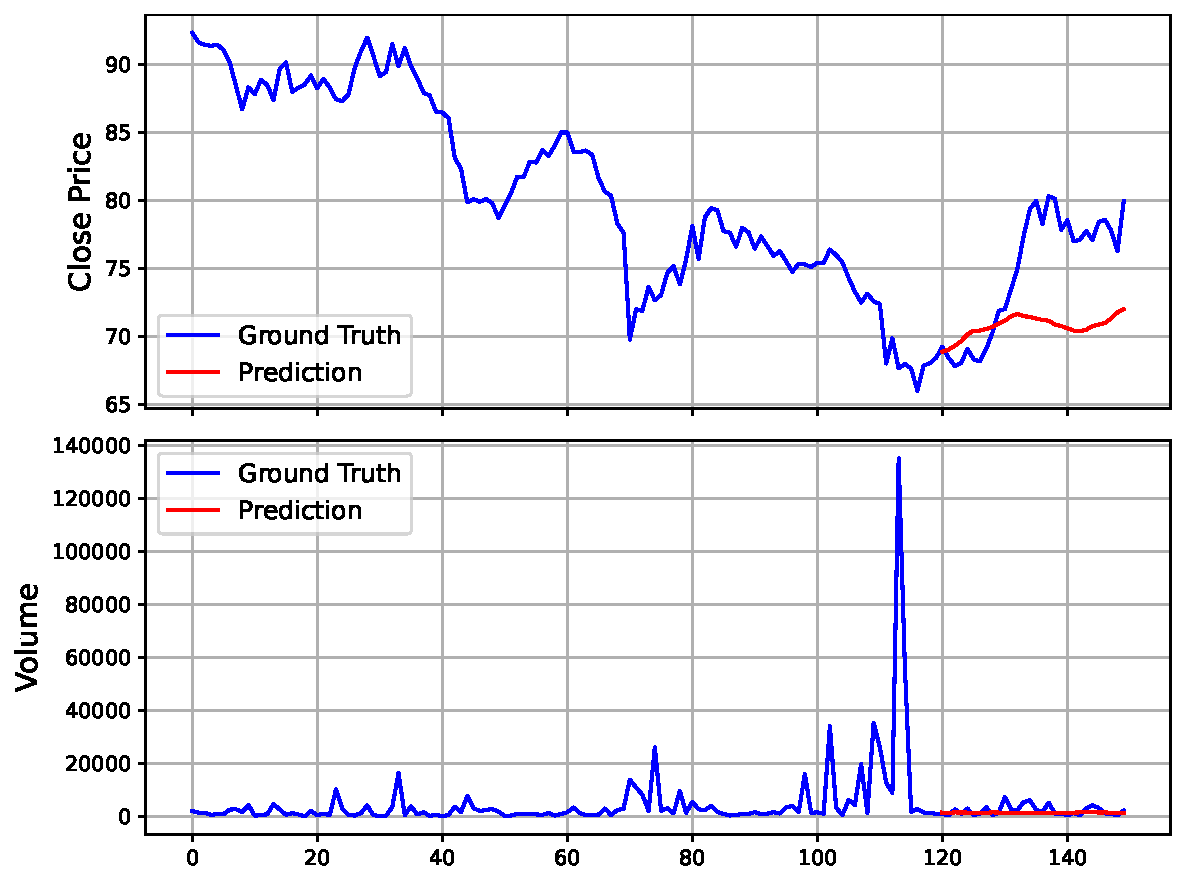
\includegraphics[width=\linewidth]{pred_imgs/pred_visualize_stock_XFRA_BMW_daily_Chronos_base.pdf}
        \caption{$\text{Chronos}_{base}$}
    \end{subfigure}
    \hfill
    \begin{subfigure}[b]{0.33\textwidth}
        \centering
        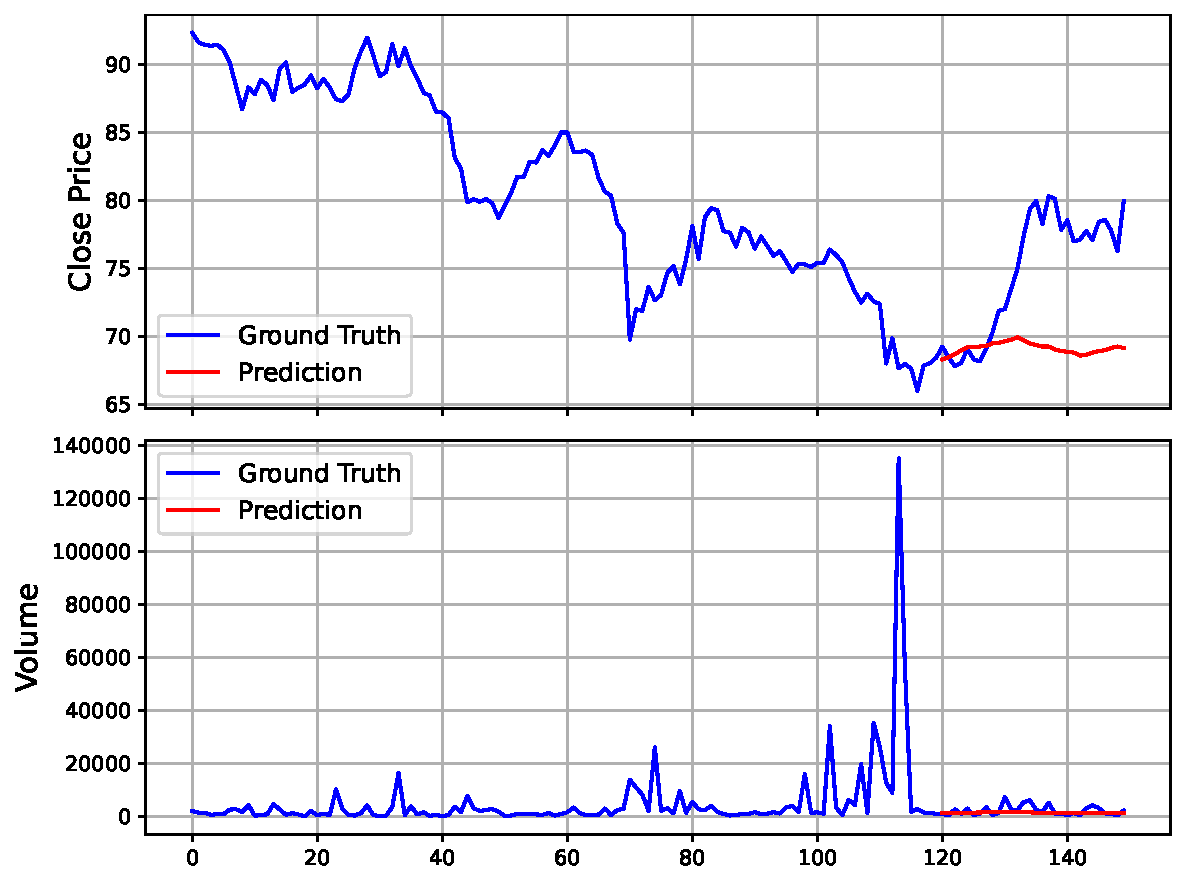
\includegraphics[width=\linewidth]{pred_imgs/pred_visualize_stock_XFRA_BMW_daily_Chronos_large.pdf}
        \caption{$\text{Chronos}_{large}$}
    \end{subfigure}

    \vspace{0.1cm}

    \begin{subfigure}[b]{0.33\textwidth}
        \centering
        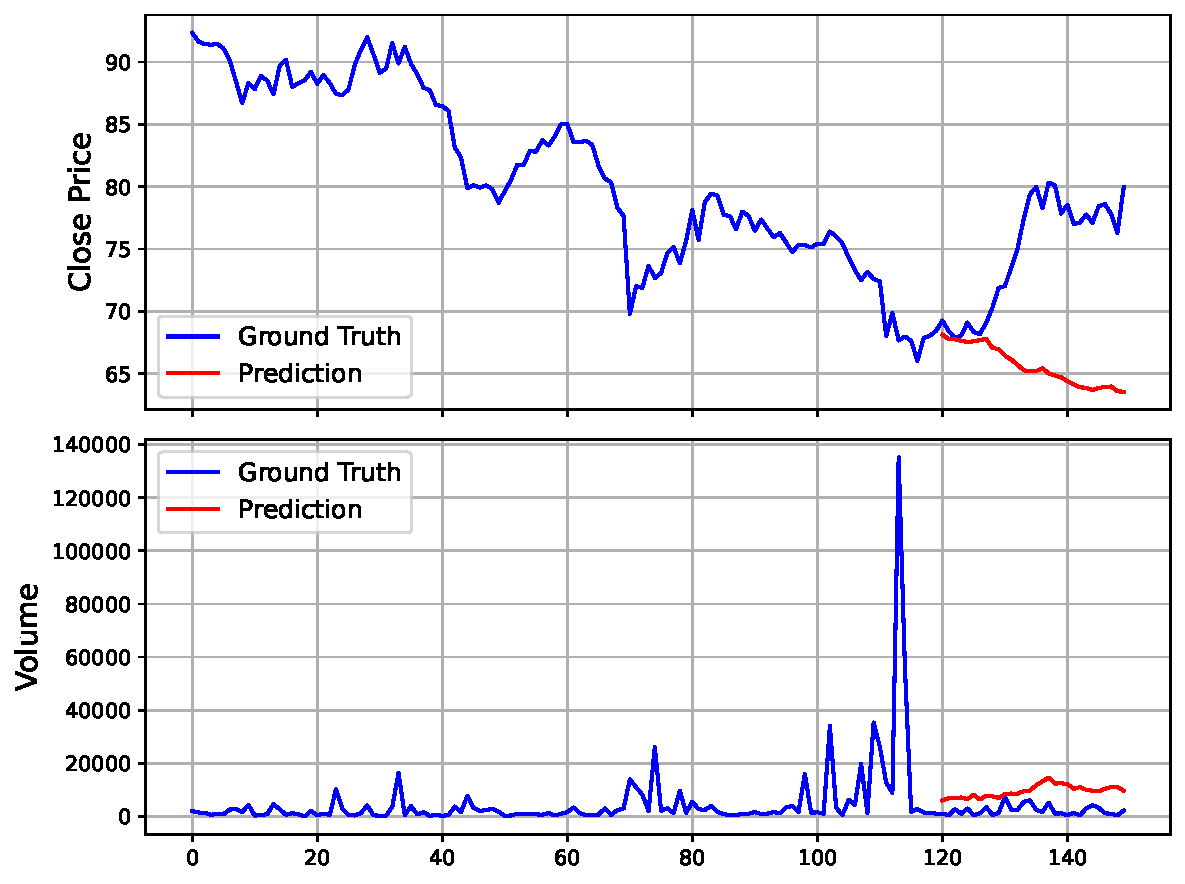
\includegraphics[width=\linewidth]{pred_imgs/pred_visualize_stock_XFRA_BMW_daily_iTransformer.pdf}
        \caption{iTransformer}
    \end{subfigure}
    \hfill
    \begin{subfigure}[b]{0.33\textwidth}
        \centering
        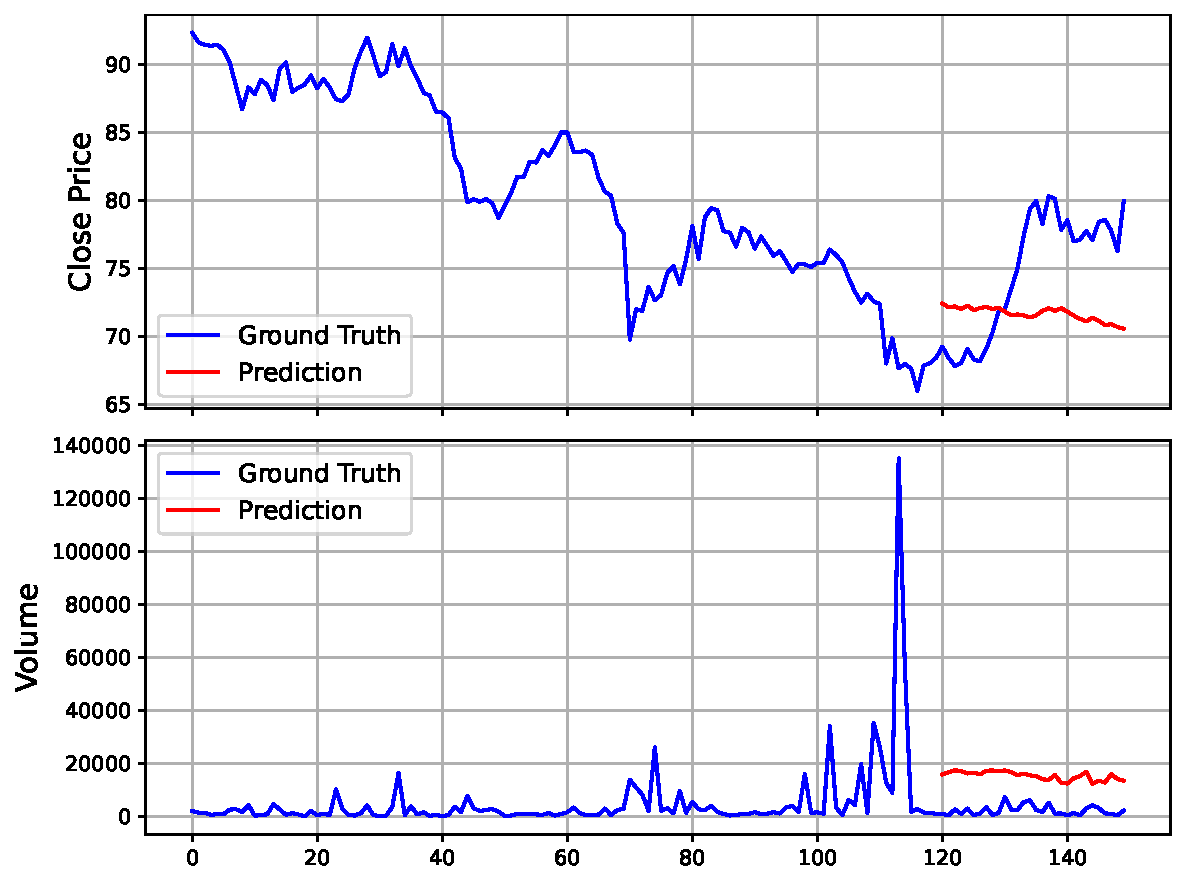
\includegraphics[width=\linewidth]{pred_imgs/pred_visualize_stock_XFRA_BMW_daily_DLinear.pdf}
        \caption{DLinear}
    \end{subfigure}
    \hfill
    \begin{subfigure}[b]{0.33\textwidth}
        \centering
        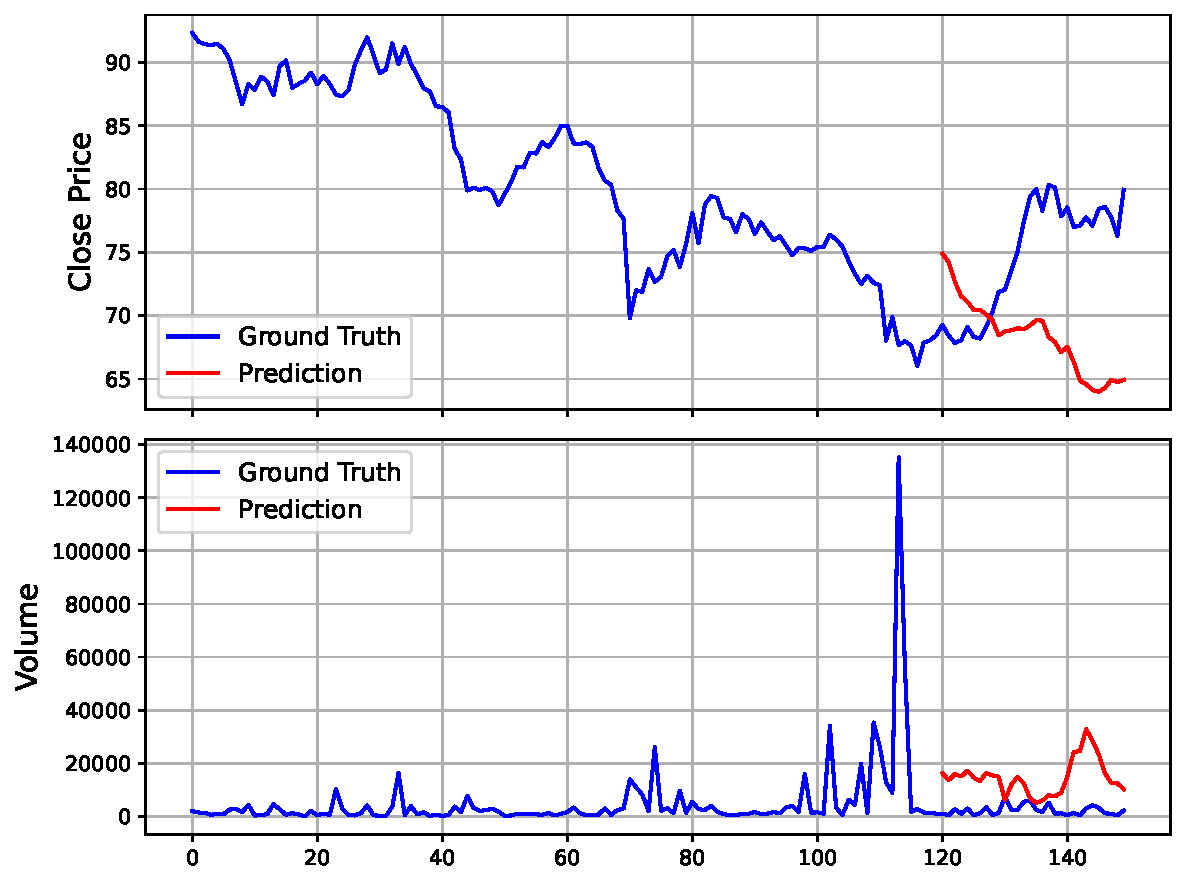
\includegraphics[width=\linewidth]{pred_imgs/pred_visualize_stock_XFRA_BMW_daily_TimesNet.pdf}
        \caption{TimesNet}
    \end{subfigure}

    \caption{일간 K-line 데이터를 기반으로 한 BMW (FWB: BMW)의 `Close Price'와 `Volume' 예측 결과. 모델은 120스텝 look-back 윈도우를 사용하여 30스텝 horizon을 예측한다. \textcolor{blue}{Blue} 선은 정답값을 나타내고 \textcolor{red}{red} 선은 모델의 예측값을 나타낸다.}
    \label{fig:pred_case_5}
\end{figure*}
